%   =============================
%		Change document settings here 
%   =============================

% TITLEPAGE SETTINGS
% ------------------
\newcommand{\docAutor}					{Ingo B�rk}								% name of the author of the book
\newcommand{\docTitel}					{Stochastische Prozesse}	% title of the lecture/book
\newcommand{\docUntertitel}			{Skript vom Wintersemester 2011/2012}					% subtitle
\newcommand{\docDozent}					{Prof. Ingo Steinwart}		% name of the professor
\newcommand{\docJahr}						{2011}										% publishing year
\newcommand{\docUniversitaet}		{Universit�t Stuttgart}		% name of university
\newcommand{\docTitelZitat}			{Mathematics, rightly viewed, possesses not only truth, but supreme beauty.}
\newcommand{\docTitelZitatName}	{Bertrand Russell}				% titlepage quote author

% GENERAL SETTINGS
% ----------------
\newcommand{\useIndex}					{1} 											% set '1' if you want to include an index
\newcommand{\useThumbs}					{0}												% set '1' if you want to use chapter thumbs on the page side
\newcommand{\useRoman}					{0}												% set '1' if you want to have chapter numbering with roman numbers

\newcommand{\usrBCOR}						{0cm} 										% set binding correction offset here (space lost on the inner borders due to binding)
\newcommand{\usrmatter}					{0}												% set '1' to start numbering at actual content beginning
\newcommand{\usroptsqrt}				{1}												% set '1' to use alternate form for roots with a small closing line
\newcommand{\usrnscmd}[1]				{\textbf{#1}}							% set e.g. '\textbf', '\mathbb' or '\mathds' for namespace macros
				% document specific settings

\documentclass[a4paper, 						% paper size
							 12pt, 								% font size
							 BCOR = \usrBCOR,			% binding correction
							 DIV=15, 							% used for typearea calculation
							 headsepline,					% add head line to border calculation
							 twoside, 						% two-sided document
							 footnotes = multiple,% visually separate two consecutive footnotes
							 toc = index,					% add index to table of contents
							 numbers = auto,			% automatic placing of end dot in numbering
							 pagesize							% used for flexibility
							]{scrbook}						% KOMA book class
							
\input{inc/settings/preamble}				% general settings and packages
\input{inc/settings/abbreviations}	% predefined macros
\input{inc/settings/environments}		% predefined environments
\input{inc/settings/hyphenation}		% custom hyphenation rules

%\includeonly{}											% while writing your book, compile only what you need

\begin{document}
\raggedbottom
\ifthenelse{\equal{\usrmatter}{1}}
	{\frontmatter}{}
\include{inc/titlepage}
\newpage
\thispagestyle{empty}

\markboth{Rechtshinweise}{Rechtshinweise}

\noindent Dieses Skript entstand im Rahmen der Vorlesung "`\docTitel"' bei \docDozent\ als Vorlesungsmitschrieb.

Es kann nicht garantiert werden, dass dieses Dokument fehlerfrei ist und der Autor �bernimmt f�r m�glicherweise entstandene Sch�den jeglicher Art keine Haftung. Dieser Mitschrieb ist kein offizielles Dokument der \docUniversitaet, Mitarbeiter eben dieser tragen daher ebenfalls keine Verantwortung.

Dieses Werk ist unter dem Lizenzvertrag "`Creative Commons Attribution-NonCommercial-ShareAlike 3.0 Germany"' lizenziert. Um die Lizenz anzusehen, gehen Sie bitte auf die Webseite http://creativecommons.org/licenses/by-nc-sa/3.0/de/ oder schicken Sie einen Brief an:

\vspace{1em} 
\begin{minipage}{0.8\textwidth}
\addtolength{\leftskip}{1em}
Creative Commons,\\ 
171 Second Street,\\ 
Suite 300,\\ 
San Francisco,\\ 
California 94105, USA.
\end{minipage}
\vspace{1em}

\noindent Mit freundlichen Gr��en\\
\docAutor
\newpage
\tableofcontents
\cleardoublepage
\thispagestyle{scrplain}
\markboth{Vorwort}{Vorwort}
\addcontentsline{toc}{chapter}{Vorwort}

\vphantom{\fontsize{50}{0}\selectfont 1}
\vphantom{\Huge A}
\begin{flushright}\normalfont\sffamily\Huge\bfseries Vorwort\end{flushright}
\vspace{1cm}
Mittels eines \emph{stochastischen Prozesses} beschreibt man in der Mathematik zeitlich geordnete, zuf�llige Vorg�nge. Die Theorie dieser Prozesse erweitert die Wahrscheinlichkeitstheorie und �ffnet das Tor zur stochastischen Analysis. 
\ifthenelse{\equal{\usrmatter}{1}}
	{\mainmatter}{}
\ifthenelse{\equal{\useThumbs}{1}}
	{\ihead[\putchapterthumb]{\putchapterthumb}}{}
	
% ================================
% include your document parts here
% only use section-wise documents since include inserts new pages!
\chapter{�bersicht und Einf�hrung}

\begin{beschreibung}
In diesem Kapitel wollen wir die grundlegenden Begriffe f�r die stochastischen Prozesse definieren, eine kurze Einf�hrung in die Thematik geben und einfache Eigenschaften herleiten.
\end{beschreibung}

\section{Stochastische Prozesse}

Im ersten Schritt wollen wir uns den namensgebenden Begriff anschauen und festlegen, was wir unter einem stochastischen Prozess verstehen:

\begin{definition}[Stochastischer Prozess]\label{Nummer1.1.1}
Sei $(\Omega, \sA, P)$ ein Wahrscheinlichkeitsraum, $(\sX, \sB)$ ein Messraum und $T \neq \emptyset$. Dann hei�t eine Familie $X = (X_t)_{t \in T}$ mit f�r alle $t \in T$ messbaren Funktionen $X_t\colon \Omega \to \sX$ ein \deftxt{stochastischer Prozess}\index{Stochastischer Prozess}.
\end{definition}

Da der Begriff die Grundlage f�r die ganze Thematik darstellt, werden wir desweiteren einige Eigenschaften kennenlernen, um verschiedene Arten von stochastischen Prozessen zu unterscheiden.

\begin{klassifikation}\label{Nummer1.1.2}
Wir legen folgende klassifizierenden Eigenschaften f�r stochastische Prozesse fest:
\begin{itemize}
	\item Ist $\sX = \R$, so sprechen wir von \deftxt{reellwertigen}\index{Stochastischer Prozess!reellwertiger} stochastischen Prozessen.
	\item Ein stochastischer Prozess mit endlichem/abz�hlbarem \deftxt{Zustandsraum}\index{Zustandsraum} $\sX$ hei�t selbst \deftxt{endlich}\index{Stochastischer Prozess!endlicher}/\deftxt{abz�hlbar}\index{Stochastischer Prozess!abz�hlbarer}.
	\item Ist $\sX = \R^d$, so sprechen wir von einem \deftxt{Punktprozess}\index{Punktprozess}.
	\item Ist $T \in \{\N, \N_0, \Z\}$, so nennen wir den Prozess einen \deftxt{zeitdiskreten}\index{Stochastischer Prozess!zeitdiskreter} stochastischen Prozess.
	\item Falls $T \subset \R$ ein Intervall ist, so sprechen wir von einem \deftxt{zeitkontinuierlichen}\index{Stochastischer Prozess!zeitkontinuierlicher} stochastischen Prozess.
\end{itemize}
\end{klassifikation}

Wir werden uns im Wesentlichen jedoch auf zeitdiskrete/kontinuierliche stochastische Prozesse mit Zustandsraum $\R$ oder h�chstens abz�hlbaren Mengen beschr�nken, es gibt in der Theorie jedoch noch viel mehr F�lle wie z.\,B. Mengen von Funktionen als Zustandsraum.

\begin{beispiel*}[Bereits bekannte stochastische Prozesse]
Stochastische Prozesse sind zu diesem Zeitpunkt keine v�llig neuartigen Objekte, wir kennen bereits folgende Vertreter:
\begin{itemize}
	\item $(X_n)_{n \in \N}$ mit i.\,i.\,d. Zufallsvariablen $X_n$.
	\item $(\overline{X_n})_{n \in \N}$ f�r eine Folge von i.\,i.\,d. Zufallsvariablen $(X_n)_{n \in \N}$ mit $\overline{X_n} = \frac{1}{n}\sum_{i=1}^n X_i$.
	\item $(X_n^*)_{n \in \N}$ f�r i.\,i.\,d. Zufallsvariablen $X_n$ mit $X_n \in \sL_2$ und $\sigma^2 := \Var X_1 > 0$, sowie
	\begin{align*}
	X_n^* &:= \frac{1}{\sqrt{n\sigma^2}} \sum_{i=1}^n (X_i - \E X_i)\text{.}
	\end{align*}
\end{itemize}
Seien $(X_i)_{i \in \N}$ i.\,i.\,d. mit $X_1 \in \sL_2$ und $\Var X_1 > 0$, dann ist $(\overline{X_n})_{n \in \N}$ weder unabh�ngig noch identisch verteilt und $(X_n^*)_{n \in \N}$ nicht unabh�ngig, aber eventuell identisch verteilt.
\end{beispiel*}

\begin{definition}[Pfad/Trajektorie]\label{Nummer1.1.3}
Sei $X = (X_t)_{t \in T}$ ein stochastischer Prozess, dann hei�t f�r $\omega \in \Omega$ die Abbildung
\begin{align*}
X(\omega)\colon T &\to \sX\text{,}\\
t &\mapsto X_t(\omega)
\end{align*}
\deftxt{Pfad}\index{Pfad} oder \deftxt{Trajektorie}\index{Trajektorie} von $X$ bez�glich $\omega$.
\end{definition}

Stochastische Prozesse erzeugen also zuf�llige Abbildungen von $T$ in den Zustandsraum $\sX$. Abh�ngig von der Klasse des Prozesses (zeitdiskret, zeitkontinuerlich, \ldots) ist die erzeugte Funktion mitunter eine Folge oder eine "`normale"' reellwertige Funktion.

\begin{lemma}\label{Nummer1.1.4}
Wir betrachten die Menge $\sX^T := \bigtimes_{t \in T} \sX$ der Abbildungen $T \to \sX$, ausgestattet mit der Produkt-$\sigma$-Algebra $\sB^T := \bigotimes_{t \in T} \sB$. Ferner sei $X = (X_t)_{t \in T}$ ein $\sX$-wertiger stochastischer Prozess �ber $(\Omega, \sA, P)$. Dann ist
\begin{align*}
X\colon \Omega &\to \sX^T\text{,}\\
\omega &\mapsto X(\omega) = (t \mapsto X_t(\omega))
\end{align*}
eine messbare Abbildung, das hei�t $X$ ist eine $\sX^T$-wertige Zufallsvariable.
\end{lemma}

\begin{beweis}
Die Aussage des Lemma folgt unmittelbar aus \cite[Lemma I.9.16]{WT}.
\end{beweis}

Wir haben nun zwar einen neuen Begriff, allerdings noch kein Ziel, das wir anstreben. Daher wollen wir nun auf einige typische Fragestellungen eingehen. H�ufig wird untersucht, ob die Trajektorien beschr�nkt sind, wie ihr Wachstumsverhalten aussieht, ob sie f�r $t \to \infty$ konvergieren, ob sie stetig sind, wann ihre Austrittszeiten sind (d.\,h. wann verl�sst der Pfad ein gewisses Intervall) et cetera.

Stochastische Prozesse finden in vielen Gebieten breite Anwendung. Beispiele f�r typische Anwendungsfelder f�r stochastische Prozesse sind:
\begin{enumerate}
	\item \emph{Finanzmathematik} -- Bewertung von Finanzprodukten, Risikomangement, Investitionsstrategien
	\item \emph{Physik} -- Diffusionssysteme, stochastische Thermodynamik, Quantenphysik
	\item \emph{Biologie} -- Populationsmodelle, "`Genomics"'
	\item \emph{Ingenieurswissenschaften} -- Warteschlangenprobleme, Steuerungsprobleme
\end{enumerate}
	\section{Einfache Eigenschaften}

Wir wollen zun�chst einige einfache Eigenschaften stochastischer Prozesse untersuchen. Die erste Eigenschaft bezieht sich auf die Gleichheit stochastischer Prozesse, dazu seien $X = (X_t)_{t \in T}$ und $Y = (Y_t)_{t \in T}$ zwei $\sX$-wertige stochastische Prozesse �ber dem gleichen Wahrscheinlichkeitsraum $(\Omega, \sA, P)$. Als Abbildungen $\Omega \times T \to \sX$ w�rden wir Gleichheit durch $X_t(\omega) = Y_t(\omega)$ f�r alle $t \in T$ und alle $\omega \in \Omega$ definieren. Da wir mit stochastischen Prozessen nach Lemma \ref{Nummer1.1.4} jedoch auch Zufallsvariablen vorliegen haben, wollen wir auch andere Begriffe f�r die Unterscheidbarkeit einf�hren.

\begin{definition}[Unterscheidbarkeit]\label{Nummer1.2.1}
Die wie eben definierten stochastischen Prozesse $X$ und $Y$ hei�en \deftxt{nicht unterscheidbar}\index{Unterscheidbarkeit} genau dann, wenn f�r $P$-fast alle $\omega \in \Omega$ und f�r alle $t \in T$ die Gleichheit $X_t(\omega) = Y_t(\omega)$ gilt. Dies ist genau dann der Fall, wenn $P(\{\omega: X(\omega) = Y(\omega)\}) = 1$ gilt.\\
Die Prozesse sind also nicht unterscheidbar, wenn fast alle Pfade gleich sind.
\end{definition}

Die Aussage ist also, dass Prozesse nicht unterscheidbar sind, wenn es eine von $t$ unabh�ngige Nullmenge gibt, au�erhalb welcher die Pfade �bereinstimmen. Wir wollen jetzt gewisserma�en die Reihenfolge der Quantoren vertauschen und zulassen, dass diese Nullmenge von $t$ abh�ngt.

\begin{definition}[Version]\label{Nummer1.2.2}
Seien $X$ und $Y$ wieder wie eben definiert. Dann hei�t $X$ \deftxt{Version}\index{Version} von $Y$ (und $Y$ Version von $X$) genau dann, wenn
\begin{align*}
P(\{\omega: X_t(\omega) = Y_t(\omega)\}) &= 1 \qquad \text{f�r alle } t \in T
\end{align*}
gilt, das hei�t wir fordern Gleichheit nur noch punktweise f�r $t \in T$.
\end{definition}

\begin{lemma}\label{Nummer1.2.3}
Seien $X$ und $Y$ die zwei obigen stochastischen Prozesse. Dann gilt:
\begin{enumerate}
	\item\label{Nummer123A1} $X$ und $Y$ sind nicht unterscheidbar impliziert, dass $X$ eine Version von $Y$ ist.
	\item\label{Nummer123A2} Ist $X$ eine Version von $Y$ und $T$ abz�hlbar, so sind $X$ und $Y$ nicht unterscheidbar.
\end{enumerate}
\end{lemma}

\begin{beweis}
Der Beweis wird in den �bungen gef�hrt.
\end{beweis}

Wir wollen uns nun noch davon �berzeugen, dass diese beiden Begriffe im Allgemeinen wirklich verschieden sind. Die dahinterstehende Idee wird sein, dass eine �berabz�hlbare Vereinigung von Nullmengen im Allgemeinen keine Nullmenge mehr ist.

\begin{beispiel}\label{Nummer1.2.4}
Im Allgemeinen gilt die Umkehrung von \ref{Nummer123A1} aus Lemma \ref{Nummer1.2.3} nicht. Wir setzen $T := [0,1]$, $\Omega := [0,1]$ und $P$ sei die Gleichverteilung. Ferner sei $X_t(\omega) := 0$ f�r alle $t \in T$ und $\omega \in \Omega$, sowie $Y_t(\omega) = \begin{cases}0 & \text{f�r } t \neq \omega\\ 1 & \text{f�r } t = \omega\end{cases}$. Dann gilt f�r $t \in [0,1]$
\begin{align*}
P(\{\omega: X_t(\omega) \neq Y_t(\omega)\}) &= P(\{t\}) = 0\text{,}
\end{align*}
also ist $X$ eine Version von $Y$. Au�erdem gilt f�r jedes $\omega \in \Omega$
\begin{align*}
(t \mapsto X_t(\omega)) = X(\omega) &\neq Y(\omega) = (t \mapsto Y_t(\omega))\text{,}
\end{align*}
also sind $X$ und $Y$ unterscheidbar.
\end{beispiel}

\begin{definition}[Stetigkeit]\label{Nummer1.2.5}
Sei $X = (X_t)_{t \in T}$ ein zeitkontinuierlicher stochastischer Prozess. Dann hei�t $X$ links-/rechts- bzw. stetig genau dann, wenn $P$-fast alle Pfade (links-/rechts-)stetig sind, das hei�t f�r $P$-fast alle $\omega \in \Omega$ ist die Abbildung $X(\omega)\colon T \to \R$ (links/rechts-)stetig.
\end{definition}

Ist $X$ (links-/rechts-)stetig, so folgt, dass ein nicht unterscheidbarer stochastischer Prozess $Y$ existiert, f�r welchen \emph{alle} Pfade (links-/rechts-)stetig sind. Dazu �bernimmt man in $Y$ einfach die stetigen Pfade und ersetzt nicht-stetige $X(\omega)$ durch die Nullfunktion. Nach Voraussetzung geschieht dies nur auf einer Nullmenge, womit $X$ und $Y$ nicht unterscheidbar sind.

Stetige stochastische Prozesse sind Zufallsvariablen, deren Bild fast sicher im Raum $C(T)$ der stetigen Funktionen �ber $T$ liegt. Wie eben gesehen, finden wir damit einen nicht unterscheidbaren Prozess, dessen Bild komplett in diesem Raum liegt. 

\begin{satz}\label{Nummer1.2.6}
Seien $X$, $Y$ (links-/rechts-)stetige stochastische Prozesse und $Y$ eine Version von $X$. Dann sind $X$ und $Y$ nicht unterscheidbar.
\end{satz}

Jeder stochastische Prozess hat also bis auf Ununterscheidbarkeit h�chstens eine stetige Version.

\begin{beweis}
Ohne Einschr�nkung seien $X$ und $Y$ stetige Prozesse und $T = \R$. F�r stetige Funktionen $f, g\colon \R \to \R$ gilt die �quivalenz
\begin{align*}
f = g ~&\Leftrightarrow~ f(x) = g(x) \forall_{x \in \Q}\text{,}
\end{align*}
es gen�gt also $P\left(\left\{\omega : X_t(\omega) = Y_t(\omega) \forall_{t \in \Q}\right\}\right) = 1$ zu zeigen. Dies folgt jedoch bereits aus Lemma \ref{Nummer1.2.3} \ref{Nummer123A2} f�r $T' = \Q$.
\end{beweis}

\begin{satz}\label{Nummer1.2.7}
Sei $X = (X_t)_{t \in T}$ ein $\N_0$-wertiger und zeitkontinuierlicher stochastischer Prozess. Dann sind folgende Aussagen �quivalent:
\begin{enumerate}
	\item\label{Nummer127A1} $X$ ist rechtsstetig.
	\item\label{Nummer127A2} F�r $P$-fast alle $\omega \in \Omega$ und alle $t \in T$ existiert ein $\e > 0$ mit $X_s(\omega) = X_t(\omega)$ f�r alle $s \in [t, t + \e) \cap T$.
\end{enumerate}
\end{satz}

�ndert sich also f�r einen rechtsstetigen Prozess die Trajektorie, so verbleibt sie danach f�r eine gewisse Zeit in diesem Zustand.

\begin{beweis}
F�r die Richtung \ref{Nummer127A1} $\Rightarrow$ \ref{Nummer127A2} sei $\omega \in \Omega$ mit $X(\omega)$ rechtsstetig und $t \in T$. Wegen der rechtsseitigen Stetigkeit existiert ein $\e > 0$ mit $\left|X_t(\omega) - X_s(\omega)\right| < \frac12$ f�r alle $s \in [t, t+\e)$ und wegen $X_t(\omega) \in \N_0$ und $X_s(\omega) \in \N_0$ folgt daher $X_t(\omega) = X_s(\omega)$. Die andere Richtung des Satzes ist trivial.
\end{beweis}

Wir geben an dieser Stelle eine Klassifikation der Pfade f�r obige ($\N_0$-wertige) stochastische Prozesse:
\begin{enumerate}
	\item Der Pfad hat nur endlich viele Sprungstellen.
	\item Der Pfad hat unendlich viele Sprungstellen, aber nur endlich viele in jedem beschr�nkten Zeitintervall.
	\item Der Pfad hat unendlich viele Sprungstellen in (mindestens) einem beschr�nkten Zeitintervall.
\end{enumerate}
	\section{Endlichdimensionale Randverteilungen}

In diesem Abschnitt wollen wir stochastische Prozesse konstruieren und Gleichheit f�r unterschiedliche Wahrscheinlichkeitsr�ume diskutieren. Hierf�r ben�tigen wir jedoch die namensgebenden endlichen Randverteilungen.

\begin{definition}[Randverteilung]\label{Nummer1.3.1}
Sei $X = (X_t)_{t \in T}$ ein $\R$-wertiger stochastischer Prozess �ber dem Wahrscheinlichkeitsraum $(\Omega, \sA, P)$. Ferner seien $n \geq 1$ und $t_1, \ldots, t_n \in T$. Dann nennen wir $P_{X_{t_1}, \ldots, X_{t_n}}$, die durch
\begin{align*}
P_{X_{t_1}, \ldots, X_{t_n}}(A) &:= P\left(\left(X_{t_1}, \ldots, X_{t_n}\right) \in A\right) \qquad \text{f�r alle } A \in \sB^n
\end{align*}
definiert war, die \deftxt{Randverteilung}\index{Randverteilung} von $X$ bez�glich $t_1, \ldots, t_n$. Wir werden hierf�r die k�rzere Schreibweise $P_{t_1, \ldots, t_n}$ verwenden.
\end{definition}

\begin{satz}\label{Nummer1.3.2}
Sei $X$ ein $\R$-wertiger stochastischer Prozess �ber $(\Omega, \sA, P)$. Dann erf�llen die Randverteilungen die folgenden Eigenschaften:
\begin{enumerate}
	\item\label{Nummer132A1} \deftxt{Permutationsinvarianz}\index{Permutationsinvarianz}, das hei�t f�r jedes $n \geq 1$, jede Permutation $\pi\colon \{1, \ldots, n\} \to \{1, \ldots, n\}$ und alle $t_1, \ldots, t_n \in T$ gilt
	\begin{align*}
	P_{t_{\pi(1)}, \ldots, t_{\pi(n)}}(A) &= P_{t_1, \ldots, t_n}\left(\pi^{-1}(A)\right) \qquad \text{f�r alle } A \in \sB^n\text{,}
	\end{align*}
	wobei $\pi^{-1}(A) := \{(x_1, \ldots, x_n) : (x_{\pi(1)}, \ldots, x_{\pi(n)}) \in A\}$ ist.
	\item\label{Nummer132A2} \deftxt{Konsistenz}\index{Konsistenz}, das hei�t f�r alle $n \geq m \geq 1$ und alle $t_1, \ldots, t_n \in T$ gilt
	\begin{align*}
	P_{t_1, \ldots, t_m}(A) &= P_{t_1, \ldots, t_n}\left(A \times \R^{n-m}\right) \qquad \text{f�r alle } A \in \sB^m\text{.}
	\end{align*}
\end{enumerate}
\end{satz}

Die erste Eigenschaft besagt also, dass das gleichzeitige Permutieren der $t_i$ und $A$ keinen Effekt hat, w�hrend die zweite Eigenschaft ausdr�ckt, dass niederdimensionale Randverteilungen durch h�herdimensionale Randverteilungen ausgedr�ckt werden k�nnen.

\begin{beweis}
Wir beweisen beide Eigenschaften getrennt:
\begin{enumerate}
	\item[\ref{Nummer132A1}] Es gen�gt, Mengen der Form $A = (-\infty, a]$ f�r $a = (a_1, \ldots, a_n) \in \R^n$ zu betrachten, da diese $\cap$-stabile Erzeugendensysteme sind (vgl. \cite[Korollar I.5.3]{WT}). Es gilt
	\begin{align*}
	\pi^{-1}(A) &= \left\{(x_1, \ldots, x_n) : x_{\pi(i)} \leq a_i \quad \forall_{i = 1, \ldots, n}\right\}\text{.}
	\end{align*}
	Daraus folgt dann
	\begin{align*}
	P_{t_{\pi(1)}, \ldots, t_{\pi(n)}}(A) &= P\left(X_{t_{\pi(i)}} \leq a_i \quad \forall_{i = 1, \ldots, n}\right)\\
	\quad &= P_{t_1, \ldots, t_n}\left(\pi^{-1}(A)\right)\text{.}
	\end{align*}
	\item[\ref{Nummer132A2}] Diese Aussage folgt wegen
	\begin{align*}
	P_{t_1, \ldots, t_n}(A \times \R \times \ldots \times \R) &= P\left(X_{t_i} \in A \quad \forall_{i = 1, \ldots, m} \quad\text{und}\quad X_{t_i} \in \R \quad \forall_{i = m+1, \ldots, n}\right)\\
	\quad &= P_{t_1, \ldots, t_m}(A)\text{.} \qedhere
	\end{align*}
\end{enumerate}
\end{beweis}

\begin{satz}[Existenzsatz von Kolmogorov]\label{Nummer1.3.3}\index{Existenzsatz (Kolmogorov)}
Sei $T \neq \emptyset$ und $\sP = \left(P_{t_1, \ldots, t_n}\right)_{t_1, \ldots, t_n \in T}$ eine Familie von Wahrscheinlichkeitsma�en, so dass $P_{t_1, \ldots, t_n}$ ein Wahrscheinlichkeitsma� auf $\R^n$ ist. Ferner sei $\sP$ permutationsinvariant und konsistent. Dann gibt es einen $\R$-wertigen stochastischen Prozess $X = (X_t)_{t \in T}$, f�r welchen die Familie $\sP$ die Familie der endlichdimensionalen Randverteilungen ist, das hei�t
\begin{align*}
P_{X_{t_1}, \ldots, X_{t_n}} &= P_{t_1, \ldots, t_n} \quad \text{f�r alle } n \geq 1 \text{ und } t_1, \ldots, t_n \in T\text{.}
\end{align*}
\end{satz}

Permutationsinvariante, konsistente Familien definieren also einen stochastischen Prozess. Wir werden den Satz hier nicht beweisen, da der Beweis zu sehr in andere Fachgebiete reicht. Er findet sich in \cite[Korollar A.20]{MEINTRUP}.

\begin{information}
In der Literatur wird h�ufig $\sP = (P_I)_{I \subset T}$ mit endlichen $I$ betrachtet. Die Permutationsinvarianz ist hier gewisserma�en bereits eingebaut und wird daher nicht mehr extra erw�hnt. 
\end{information}

\begin{definition}[Gleiche Randverteilung]\label{Nummer1.3.4}
Seien $X = (X_t)_{t \in T}$ und $Y = (Y_t)_{t \in T}$ zwei $\R$-wertige stochastische Prozesse �ber $(\Omega, \sA, P)$ bzw. $(\Omega', \sA', P')$. Dann haben $X$ und $Y$ die \deftxt{gleichen Randverteilungen}\index{Randverteilung!gleiche} genau dann, wenn
\begin{align*}
P_{X_{t_1}, \ldots, X_{t_n}} &= P_{Y_{t_1}, \ldots, Y_{t_n}} \quad \text{f�r alle } n \geq 1 \text{ und } t_1, \ldots, t_n \in T
\end{align*}
gilt. Wir schreiben hierf�r $X \stackrel{\mathrm{d}}{=} Y$.
\end{definition}

Wenn $X$ eine Version von $Y$ ist, so folgt insbesondere $X \stackrel{\mathrm d}{=} Y$. Wir �berlassen den Beweis hierf�r jedoch dem Leser. Der stochastische Prozess aus Satz \ref{Nummer1.3.3} ist bis auf "`$\stackrel{\mathrm d}{=}$"' eindeutig.

\Needspace{4\baselineskip}\begin{definition}[Station�rer Prozess]\label{Nummer1.3.5}
Ein $\R$-wertiger stochastischer Prozess $(X_t)_{t \in T}$ hei�t \deftxt{station�r}\index{Stochastischer Prozess!station�rer} genau dann, wenn $T$ bez�glich $+$ abgeschlossen ist und f�r alle $n \geq 1$ und alle $t_1, \ldots, t_n, s \in T$ gilt:
\begin{align*}
P_{t_1 + s, \ldots, t_n + s} &= P_{t_1, \ldots, t_n}
\end{align*}
\end{definition}

Randverteilungen �ndern sich bei station�ren stochastischen Prozessen also nicht mit der Zeit. 

\begin{definition}[Zuw�chse]\label{Nummer1.3.6}\index{Zuwachs}
Ein $\R$-wertiger stochastischer Prozess $(X_t)_{t \in T}$ hat
\begin{enumerate}
	\item \deftxt{unabh�ngige Zuw�chse}\index{Zuwachs!unabh�ngiger} genau dann, wenn f�r alle $n \geq 1$ und $t_0 < t_1 < \ldots < t_n$ die Zufallsvariablen $X_{t_1} - X_{t_0}, \ldots, X_{t_n} - X_{t_{n-1}}$ unabh�ngig sind.
	\item \deftxt{station�re Zuw�chse}\index{Zuwachs!station�rer} genau dann, wenn $T$ bez�glich $+$ abgeschlossen ist und f�r alle $r, s, t \in T$ gilt:
	\begin{align*}
	X_{r+s+t} - X_{r+t} &\stackrel{\mathrm d}{=} X_{r+s} - X_r
	\end{align*}
	Das hei�t der Zuwachs innerhalb der Zeit $s$ �ndert sich nicht durch zeitliche Verschiebung.
\end{enumerate}
\end{definition}
	\section{Einfache Beispiele}

\begin{beispiel}[Unabh�ngig und identisch verteilt]\label{Nummer1.4.1}
Sei $X = (X_n)_{n \geq 1}$ i.\,i.\,d. Dann gilt:
\begin{enumerate}
	\item\label{Nummer141A1} Die Randverteilungen sind gerade die Produktma�e (siehe auch "`Kanonisches Modell"' in \cite[Satz II.2.5]{WT}).
	\item\label{Nummer141A2} $X$ ist station�r.
	\item\label{Nummer141A3} $X$ hat station�re Zuw�chse.
	\item\label{Nummer141A4} $X$ hat im Allgemeinen keine unabh�ngigen Zuw�chse.
\end{enumerate}
Die Aussagen \ref{Nummer141A2} und \ref{Nummer141A3} folgen aus \ref{Nummer141A1}, \ref{Nummer141A4} wird dem Leser zum Beweis �berlassen.
\end{beispiel}

\begin{beispiel}[Irrfahrt]\label{Nummer1.4.2}
Es sei $(Y_n)_{n \geq 0}$ ein i.\,i.\,d. stochastischer Prozess mit $Y_n \sim \Binom\left(1, \frac12\right)$. Dann hei�t $X = (X_n)_{n \geq 0}$ mit $X_n := \sum_{i=0}^n Y_i$ f�r $n \geq 0$ \deftxt{symmetrische Irrfahrt}\index{Irrfahrt!symmetrische}. Ist $Y_n \sim \Binom(1, p)$ f�r $p \in [0,1]$, so sprechen wir von einer \deftxt{asymmetrischen}\index{Irrfahrt!asymmetrische} Irrfahrt. Der Prozess $X$ hat station�re und unabh�ngige Zuw�chse, ist jedoch nicht station�r.

Zun�chst gilt f�r $m < n$, dass
\begin{align*}
X_n - X_m = \sum_{i=m+1}^n Y_i \tag{*}\label{Nummer142E1}
\end{align*} 
ist. Da die $Y_i$ unabh�ngig sind, folgt die Unabh�ngigkeit der Zuw�chse aus \cite[Satz II.2.7, Satz II.2.9]{WT} und der Tatsache, dass kein Index $i$ doppelt vorkommt. Die Stationarit�t der Zuw�chse folgt ebenfalls aus \eqref{Nummer142E1}. Da $X_n \sim \Binom(n, p)$ gilt sind die eindimensionalen Randverteilungen nicht gleich, d.\,h. $P_n \neq P_{n+1}$.\\
In der Regel wird die symmetrische Irrfahrt jedoch anders definiert, da man in beide Richtungen gehen k�nnen m�chte. Man setzt hierf�r $Z_n := \sum X_n - 1$. Dies entspricht der Summe von Zufallsvariablen mit Werten in $\{\pm 1\}$.

Die Irrfahrt wird u.\,a. zur Untersuchung von einfachen Wettspielen verwendet. Beispielsweise gebe es zwei Spieler und eine M�nze, die wiederholt geworfen wird. Falls sie Kopf zeigt, so verliert Spieler 1 und zahlt seinem Kontrahenten einen Euro, entsprechend umgekehrt f�r den Fall "`Zahl"'. Man kann sich nun fragen, wie lange es dauert, bis einer der Spieler pleite ist (ein gewisses Startkapital sei gegeben) oder wie gro� die Wahrscheinlichkeit daf�r ist, dass Spieler 1 verliert et cetera. \qedhere
\begin{figure}[!htb]
\centering
\begin{tikzpicture}
\draw[->, semithick] (0, -0.5) -- (0, 4);
\draw[->, semithick] (-0.5, 0) -- (7.5, 0);
\draw[circle, fill=blue] (0, 3) circle (2pt) node (AK) {};
\node[rotate=90] (Sp1) at (-0.5, 3) {\small Anfangskapital};
\draw[blue, semithick] (0, 3) -- (1, 2) -- (2, 3) -- (3, 2) -- (4, 1) -- (5, 2) -- (6, 1) -- (7, 0); 
\draw[circle, fill=blue] (7,0) circle (2pt) node (Pleite2) {};
\node (Pleite1) at (8, 1.5) {\small Pleite};
\draw[->] (Pleite1) to[out=-90, in=80] (Pleite2);
\end{tikzpicture}
\caption[Darstellung einer Irrfahrt]{Darstellung einer Wettspiel-Irrfahrt f�r einen Spieler.}\label{irrfahrt}
\end{figure}
\end{beispiel}

\begin{beispiel}[Gleitendes Mittel]\label{Nummer1.4.3}
Es sei $(X_n)_{n \in \Z}$ ein $\R$-wertiger stochastischer Prozess, $k \in \N$ und $c_0, \ldots, c_k \in [0,1]$ mit $\sum_{i=0}^k c_i = 1$. Wir definieren nun $Y = (Y_n)_{n \in \Z}$ verm�ge $Y_n := \sum_{i=0}^k c_i X_{n-i}$. Dann hei�t $Y$ \deftxt{gleitendes Mittel}\index{gleitendes Mittel} von $X$ bez�glich der Gewichtung $c_0, \ldots, c_k$. Gleitende Mittel gl�tten den Prozess $X$ gewisserma�en und werden unter anderem bei der Zeitreihenanalyse eingesetzt (z.\,B. Aktienkurse). Der Prozess $Y$ ist station�r. Gilt zudem, dass $(X_n)_{n \in \Z}$ i.\,i.\,d. mit $X_i \in \sL_2$ ist, so ist $\Var Y_n \leq \Var X_n$, wobei die echte Ungleichung in der Mehrzahl der F�lle gilt. Der Beweis f�r diese Eigenschaften wird dem Leser �berlassen.
\end{beispiel}

\begin{beispiel}[Untypisches Beispiel]\label{Nummer1.4.4}
Es sei $P = \bigotimes_{i=1}^\infty \lambda_{[0,1]}$ auf $[0,1]^\N$, ausgestattet mit der Produkt-$\sigma$-Algebra. Wir definieren f�r $\omega \in [0,1]$, also eine Folge $\omega = (\omega_i)_{i \geq 1}$, und $t \in [0, \infty)$ die Zufallsvariablen
\begin{align*}
X_t(\omega) &:= \sum_{i=1}^\infty \frac{\omega_i}{i!}t^i\text{.}
\end{align*}
Die Reihe konvergiert absolut und gleichm��ig auf allen Kompakta. Ferner bildet $X = (X_t)_{t \geq 0}$ einen stochastischen Prozess und jede Trajektorie $X(\omega) = (t \mapsto X_t(\omega))$ ist eine analytische Funktion. Ist also $X_t(\omega)$ f�r alle $t \in (t_1, t_2)$ bekannt, so ist bereits die gesamte Trajektorie bekannt. 
\end{beispiel}

Solche Prozesse wie in Beispiel \ref{Nummer1.4.4} interessieren uns hier allerdings nicht, weshalb wir sie nicht mehr betrachten werden. Stattdessen haben die Prozesse, die wir betrachten werden, eine wesentlich lockerere Beziehung zwischen Vergangenheit und Zukunft. Daf�r m�ssen wir jedoch erst mehr Theorie entwickeln.
	\section{Bedingte Erwartungen}\label{sec:BedErw}

Dieses Kapitel ist von \emph{zentraler} Wichtigkeit f�r alles, was wir machen werden. Wir verweisen an dieser Stelle daher explizit auf \cite[Kapitel 8]{MEINTRUP} und \cite{KLENKE}.

Bisher hatten wir bedingte Wahrscheinlichkeiten durch $P(B~|~A) := \frac{P(A \cap B)}{P(A)}$ definiert, sofern $P(A) > 0$ gilt. Die Interpretation war, dass $P(B~|~A)$ die Wahrscheinlichkeit f�r $B$ beschreibt, falls $A$ eintritt. Dies wollen wir auf zwei Weisen verallgemeinern:
\begin{enumerate}
	\item Es soll $P(A) = 0$ erlaubt sein.
	\item Es soll mehr als ein Ereignis $A$ erlaubt sein.
\end{enumerate}
Der Hintergrund hierf�r ist folgender: Sind $X$ und $Y$ zwei $\R$-wertige Zufallsvariablen, so wollen wir Fragen beantworten wie zum Beispiel:
\begin{enumerate}
	\item Wie gro� ist die Wahrscheinlichkeit von $Y \in B$, falls $X(\omega)$ eintritt? Die Wahrscheinlichkeiten solcher Elementarereignisse verschwinden sehr oft, weshalb wir die erste Verallgemeinerung ben�tigen.
	\item Wie gro� ist die Wahrscheinlichkeit von $Y \in B$, falls f�r $\omega \in \Omega$ und jedes $A \in \sB = \sigma(X)$ bekannt ist, ob $X(\omega) \in A$ gilt?
\end{enumerate}
Wir w�hlen die "`heuristische"' Herangehensweise. Es sei $(\Omega, \sA, P)$ ein Wahrscheinlichkeitsraum, $Y \in \sL_1(P)$, $A \in \sA$ mit $P(A) > 0$ und $X\colon \Omega \to \R$ messbar. Wir setzen nun
\begin{align*}
\E(Y~|~A) &:= \frac{\E(Y \cdot \ind_A)}{P(A)} \tag{*}
\end{align*}
und verallgemeinern dadurch $P(B~|~A)$, denn es gilt
\begin{align*}
\E(\ind_B ~|~ A)  &= \frac{\E(\ind_B \cdot \ind_A)}{P(A)} = \frac{\E(\ind_{A \cap B})}{P(A)} = \frac{P(A \cap B)}{P(A)}\\
									&= P(B~|~A)\text{.}
\end{align*}
Nun betrachten wir f�r $x \in \R$ die Menge $A_x := \{\omega: X(\omega) = x\}$. Daf�r nehmen wir an, dass $X$ diskret verteilt ist, das hei�t, es existieren h�chstens abz�hlbar viele $x \in X$ mit $P(A_x) > 0$ und $\sum_{x \in X} P(A_x) = 1$. Nun definieren wir $g\colon \R \to \R$ verm�ge
\begin{align*}
g(x) &:= \begin{cases}\E(Y~|~A_x) & \text{f�r } P(A_x) > 0\\ 0 & \text{sonst}\end{cases}
\end{align*}
und darauf aufbauend $Z := g \circ X$, wir erhalten also das Diagramm in \ref{bedErwKonst}.
\begin{figure}[!htb]
\centering
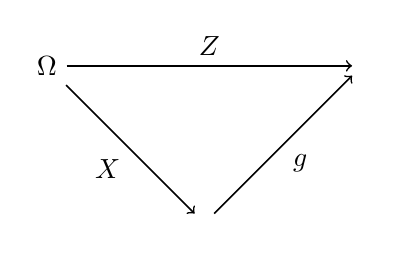
\begin{tikzpicture}
\node (Omega) at (0, 2) {$\Omega$};
\node (R1)		at (4, 2) {$\R$};
\node (R2)		at (2, 0) {$\R$};
\draw[->, semithick] (Omega) -- node[above]{$Z$} 				(R1);
\draw[->, semithick] (Omega) -- node[below left]{$X$}		(R2);
\draw[->, semithick] (R2)		 -- node[below right]{$g$}	(R1);
\end{tikzpicture}
\caption[Konstruktion der bedingten Erwartung]{Darstellung der Beziehung zwischen den R�umen und Abbildungen.}\label{bedErwKonst}
\end{figure}
Damit folgt nun, dass $Z$ $\sigma(X)$-messbar ist und �berdies gilt f�r alle $B \in \sigma(X)$:
\begin{align*}
\E(Z \cdot \ind_B) &= \int_B Z~\dd P = \int_B Y~\dd P = \E(Y \cdot \ind_B)\text{.}
\end{align*}
Also ist $Z$ eine $\sigma(X)$-messbare Zufallsvariable, die sich bez�glich Integration von $Y$ �ber $\sigma(X)$ nicht unterscheidet.

\begin{beweis}
Wir m�ssen zun�chst zeigen, dass $Z$ tats�chlich $\sigma(X)$-messbar ist. Dazu betrachten wir
\begin{align*}
Z^{-1}(\sB) &= (g \circ X)^{-1}(\sB) = X^{-1}(g^{-1}(\sB)) \subset X^{-1}(\sB) = \sigma(X)\text{,}
\end{align*}
wobei die Inklusion gilt, da $g$ messbar ist. F�r die Eigenschaft bez�glich der Integration sei zun�chst $B \in \sigma(X)$, dann existiert ein $A \in \sB$ mit $B = X^{-1}(A)$. Nun erhalten wir mit Hilfe des Transformationssatzes
\begin{align*}
\int_B Z~\dd P &= \int g \circ X \cdot \ind_A \circ X~\dd P = \int g \cdot \ind_A~\dd P_X = \sum_{x \in A} g(x)P(A_x)\\
\shortintertext{Wegen $E(Y~|~A_x) \cdot P(A_x) = \E(Y \cdot \ind_{A_x})$ erhalten wir}
						   &= \sum_{x \in A, P(A_x)>0} \E(Y \cdot \ind_{A_x}) = \E\left(Y \sum_{x \in A, P(A_x)>0} \ind_{A_x}\right)\\
\shortintertext{Da $\bigcup_{x \in A} \{\omega : X(\omega) = x\} = B$ gilt, folgt}
							 &= \E(Y \cdot \ind_B)\text{.} \qedhere
\end{align*}
\end{beweis}
Im Weiteren werden wir $Z$ mit dem eben Gesehenem definieren bzw. konstruieren und so die zweite Frage beantworten, w�hrend uns die Faktorisierung $Z = g \circ X$ die erste Frage beantworten wird.

\begin{definition}[Bedingte Erwartung]\label{Nummer1.5.1}
Es sei $(\Omega, \sA, P)$ ein Wahrscheinlichkeitsraum, $Y \in \sL_1(P)$ und $\sB \subset \sA$ eine $\sigma$-Algebra. Dann hei�t eine Zufallsvariable $Z\colon\Omega \to \R$ \deftxt{bedingte Erwartung von $Y$ unter $\sB$}\index{bedingte Erwartung}, falls gilt:
\begin{enumerate}
	\item $Z$ ist $\sB$-messbar.
	\item F�r alle $B \in \sB$ gilt
	\begin{align*}
	\E(Y \cdot \ind_B) &= \E(Z \cdot \ind_B)\text{.}
	\end{align*}
\end{enumerate}
\end{definition}

Ist $\sB = \sigma(X)$ f�r eine Zufallsvariable $X\colon \Omega \to \R$, so sind die beiden Eigenschaften der heuristischen Herangehensweise erf�llt. Zun�chst m�ssen wir uns jedoch fragen, ob es solche Objekte �berhaupt gibt und ob sie eindeutig sind.

\begin{satz}[Existenz und Eindeutigkeit]\label{Nummer1.5.2}
Es sei $(\Omega, \sA, P)$ ein Wahrscheinlichkeitsraum, $Y \in \sL_1(P)$ und $\sB \subset \sA$ eine $\sigma$-Algebra. Dann gilt:
\begin{enumerate}
	\item Es existiert eine bedingte Erwartung $Z$ von $Y$ unter $\sB$.
	\item Sind $Z$ und $Z'$ zwei bedingte Erwartungen von $Y$ unter $\sB$, so gilt $P$-fast sicher $Z = Z'$.
\end{enumerate}
\end{satz}

Bevor wir dies beweisen, wollen wir die Notation $\E(Y~|~\sB) := Z$ einf�hren. Wir nennen $Z$ \deftxt{Version}\index{Version} der bedingten Erwartung. Falls $\sB = \sigma(X)$ f�r eine Zufallsvariable $X\colon \Omega \to \R$ gilt, so schreiben wir $\E(Y~|~X) := \E(Y~|~\sigma(X))$. Es gilt zu beachten, dass $\E(\E(Y~|~\sB)\cdot\ind_B) = \E(Y \cdot \ind_B)$ f�r alle $B \in \sB$ gilt.

\begin{beweis}
Wir beweisen zun�chst die Existenz und betrachten den Fall, dass $Y \geq 0$ gilt. Dann definieren wir $\nu\colon \sB \to [0, \infty)$ durch $\nu(B) := \int_B Y~\dd P$ f�r $B \in \sB$. Dies ist ein endliches Ma�. Ferner ist $P\big|_\sB\colon \sB \to [0,1]$ ein Wahrscheinlichkeitsma� auf $\sB$ und es gilt: aus $P\big|_\sB(B) = 0$ folgt $\nu(B) = 0$. Also ist $\nu \ll P\big|_\sB$. Der Satz von Radon-Nikodym (vgl. \cite[Satz I.12.1]{WT}) gibt uns dann eine Dichte $Z\colon \Omega \to \R$ von $\nu$ bez�glich $P\big|_\sB$. Diese ist nach Konstruktion sogar $\sB$-messbar und f�r $B \in \sB$ gilt:
\begin{align*}
\int_B Z~\dd P &= \int_B \underbrace{Z~\dd P\big|_\sB}_{= \nu} = \nu(B) = \int_B Y~\dd P
\end{align*}
Im zweiten Fall sei $Y = Y^+ - Y^-$ mit $Y^+ := \max\{0, Y\} \geq 0$ und $Y^- := \max\{0, -Y\} \geq 0$. Mit Hilfe des ersten Falls erhalten wir $Z^+, Z^- \geq 0$ und setzen nun $Z := Z^+ - Z^-$.

Wir kommen nun zur Eindeutigkeit. Es seien $Z$ und $Z'$ zwei bedingte Erwartungen von $Y$ unter $\sB$. Dann gilt $\int_B Z~\dd P = \int_B Z'~\dd P$ f�r alle $B \in \sB$. Wir betrachten im Speziellen die Menge $B := \{Z > Z'\}$, die offenbar messbar ist. F�r $B$ gilt nun
\begin{align*}
0 &= \int_B \underbrace{Z - Z'}_{\geq 0}~\dd P\text{,}
\end{align*}
woraus wir $P(B) = 0$ und damit $P$-fast sicher $Z \leq Z'$ erhalten. Eine symmetrische Betrachtung durch Vertauschen der Rollen von $Z$ und $Z'$ liefert schlie�lich $P$-fast sicher $Z = Z'$.
\end{beweis}

\begin{satz}[Elementare Eigenschaften]\label{Nummer1.5.3}
Es sei $(\Omega, \sA, P)$ ein Wahrscheinlichkeitsraum, $X, Y \in \sL_1(P)$ und $\sB \subset \sA$ eine $\sigma$-Algebra. Dann gelten die folgenden Eigenschaften:
\begin{enumerate}
	\item\label{Nummer153A1} $\displaystyle \E(\E(X~|~\sB)) = \E X$.
	\item\label{Nummer153A2} Ist $X$ �berdies $\sB$-messbar, so gilt $P$-fast sicher $\E(X~|~\sB) = X$.
	\item\label{Nummer153A3} F�r $\alpha, \beta \in \R$ gilt $P$-fast sicher
	\begin{align*}
	\E(\alpha X + \beta Y ~|~ \sB) &= \alpha \E(X~|~\sB) + \beta \E(Y~|~\sB)\text{.}
	\end{align*}
	\item\label{Nummer153A4} Gilt $P$-fast sicher $X \leq Y$, so gilt auch $P$-fast sicher $\E(X~|~\sB) \leq \E(Y~|~\sB)$.
\end{enumerate}
\end{satz}

Insbesondere gilt unter den Voraussetzungen im Satz also auch $|\E(X~|~\sB)| \leq \E(|X| ~|~ \sB)$.

\begin{beweis}
Wir werden einige der Eigenschaften beweisen und die anderen dem Leser �berlassen:
\begin{enumerate}
	\item F�r $B := \Omega \in \sB$ und $Y' := \E(X~|~\sB)$ folgt $P$-fast sicher $\E Y' = \E (Y' \cdot \ind_B) = \E (X \cdot \ind_B) = \E X$.
	\item Dies folgt aus der Definition der bedingten Erwartung (Definition \ref{Nummer1.5.1}) und der Eindeutigkeit (Satz \ref{Nummer1.5.2}), denn dann ist $\E(X~|~\sB) = \E(\E(X~|~\sB) \cdot \ind_B) = \E (X \cdot \ind_B)$ f�r alle $B \in \sB$.
	\item Dieser Beweis wird dem Leser �berlassen.
	\item Es gen�gt wegen \ref{Nummer153A3} zu zeigen, dass aus $X \geq 0$ folgt, dass $\E(X~|~\sB) \geq 0$ gilt. Dies wurde jedoch bereits im Beweis von Satz \ref{Nummer1.5.2} im ersten Fall des Existenzbeweises gezeigt. \qedhere
\end{enumerate}
\end{beweis}

Wir wollen nun noch zeigen, dass die aus der Wahrscheinlichkeitstheorie bekannten Konvergenzs�tze im Wesentlichen auch f�r bedingte Erwartungen gelten.

\begin{satz}[Konvergenzs�tze]\label{Nummer1.5.4}\index{bedingte Erwartung!Konvergenzs�tze}
Es sei $(\Omega, \sA, P)$ ein Wahrscheinlichkeitsraum, $X, X_n \in \sL_1(P)$ f�r alle $n \geq 1$ und $\sB \subset \sA$ eine $\sigma$-Algebra. Dann gelten die folgenden S�tze:
\begin{enumerate}
	\item \deftxt{Satz von der monotonen Konvergenz}: Ist $P$-fast sicher $0 \leq X_n \nearrow X$, so gilt auch $\E(X_n~|~\sB) \nearrow \E(X~|~\sB)$.
	\item \deftxt{Satz von der dominierten Konvergenz}: Ist $Y \in \sL_1(P)$ mit $|X_n| \leq Y$ f�r alle $n \geq 1$ und $X_n \to X$ $P$-fast sicher, so folgt $P$-fast sicher auch $\E(X_n~|~\sB) \to \E(X~|~\sB)$. 
\end{enumerate}
\end{satz}

\begin{beweis}
Der Beweis beider S�tze erfolgt getrennt:
\begin{enumerate}
	\item Der "`normale"' Satz von Beppo Levi (vgl. Satz \ref{appendix:beppolevi1} im Anhang) liefert uns $\E(X - X_n) \to 0$. Aus Satz \ref{Nummer1.5.3} folgt dann
	\begin{align*}
	\E |\E(X~|~\sB) - \E(X_n~|~\sB)| &\stackrel{\text{\ref{Nummer153A4}}}{=} \E(\E(X~|~\sB) - \E(X_n~|~\sB)) \stackrel{\text{\ref{Nummer153A1}, \ref{Nummer153A3}}}{=} \E(X - X_n) \to 0\text{.} 
	\end{align*}
	Damit konvergiert $\E(X_n~|~\sB) - \E(X~|~\sB)$ in $\sL_1(P)$ gegen $0$. Aus der Wahrscheinlichkeitstheorie wissen wir mit \cite[Satz II.7.4]{WT}, dass dann $\E(X_n~|~\sB) - \E(X~|~\sB) \to 0$ stochastisch gilt. Aus der Wahrscheinlichkeitstheorie wissen wir, dass es dann eine Teilfolge mit $\E(X_{n_k}~|~\B) - \E(X~|~\sB) \to 0$ $P$-fast sicher gibt. Da die Folge $\E(X_{n_k}~|~\sB)$ monoton steigend ist, folgt aber auch die $P$-fast sichere Konvergenz der Gesamtfolge.
	\item Wir definieren zun�chst $Z_n := \sup_{k \geq n} |X_k - X|$, dann gilt $P$-fast sicher $Z_n \searrow 0$ und $|X_n - X| \leq Z_n$. Ferner erhalten wir
	\begin{align*}
	|\E(X_n~|~\sB) - \E(X~|~\sB)| &= |\E(X_n - X~|~\sB)| \leq \E(|X_n - X| ~|~ \sB) \leq \E(Z_n ~|~ \sB)\text{.}
	\end{align*}
	Daher werden wir nun zeigen, dass $\E(Z_n~|~\sB) \to 0$ gilt. Dazu erinnern wir uns, dass $P$-fast sicher $Z_n \searrow 0$ gilt. Daraus folgt, dass auch $\E(Z_n~|~\sB) \searrow$ gilt und wir setzen $U := \lim \E(Z_n~|~\sB)$. Klar ist, dass $U \geq 0$ gilt. Um $U = 0$ zu zeigen gen�gt es daher, $\E U = 0$ zu beweisen. Da $|X_n| \leq Y$ gilt, folgt auch $|X| \leq Y$ und damit $|X_n - X| \leq 2Y$. Nun erhalten wir $0 \leq Z_n \leq 2Y$ und der (normale) Satz von der dominierten Konvergenz\footnote{Dieser findet sich im Anhang als Satz \ref{appendix:lebesgue}.} liefert uns dann $\E Z_n \to 0$. Damit gilt $0 \leq \E U \leq \E(\E(Z_n~|~\sB)) = \E Z_n \to 0$. 
\end{enumerate}
\end{beweis}

\begin{satz}[Ungleichung von Jensen]\label{Nummer1.5.5}\index{Jensen!Ungleichung von}
Es sei $(\Omega, \sA, P)$ ein Wahrscheinlichkeitsraum, $I \subset \R$ ein Intervall, $X\colon \Omega \to I$ eine $P$-integrierbare Abbildung, $\phi\colon I \to \R$ konvex und $\sB \subset \sA$ eine $\sigma$-Algebra. Dann ist $P$-fast sicher $\E(X~|~\sB) \in I$ und gilt zus�tzlich $\phi \circ X \in \sL_1(P)$, so folgt
\begin{align*}
\phi(\E(X~|~\sB)) &\leq \E(\phi \circ X~|~\sB)\text{.}
\end{align*}
Insbesondere gilt $\phi(\E X) \leq \E (\phi \circ X)$, falls $\phi \circ X \in \sL_1(P)$ ist. 
\end{satz}

Die Ungleichung von Jensen ist also gewisserma�en eine Verallgemeinerung des Konvexit�tsbegriffes auf nicht-abz�hlbare Mengen bzw. Wahrscheinlichkeitsma�e.

\begin{beweis}
Wir setzen zun�chst $U := \{v\colon I \to \R ~|~ v\text{ ist affin linear und } v \leq \phi\}$. Dann gilt $\phi(x) = \sup_{v \in U} v(x)$ f�r alle $x \in I$. Ferner folgt $P$-fast sicher $\E(X~|~\sB) \in I$ aus $x \in I$ und der Monotonie. Au�erdem ist nun $\phi(X) = \sup_{v \in U} v(X)$. F�r $v_0 \in U$ gilt dann
\begin{align*}
v_0(\E(X~|~\sB)) &= \E(v_0 \circ X~|~\sB) \leq \E\left(\sup_{v \in U} v(X)~|~\sB\right) = \E(\phi \circ X~|~\B) 
\end{align*}  
und wir erhalten schlie�lich
\begin{align*}
\phi(\E(X~|~\sB)) &= \sup_{v \in U} v(\E(X~|~\sB)) \leq \E(\phi \circ X~|~\sB)\text{.} \qedhere
\end{align*}
\end{beweis}

\Needspace{5\baselineskip}\begin{korollar}[$\sL_p$-Zugeh�rigkeit]\label{Nummer1.5.6}
Es sei $(\Omega, \sA, P)$ ein Wahrscheinlichkeitsraum, $p \geq 1$ und $X \in \sL_p(P)$, sowie $\sB \subset \sA$ eine $\sigma$-Algebra. Dann gilt $\E(X~|~\sB) \in \sL_p(P)$ und
\begin{align*}
\norm{\E(X~|~\sB)}_{\sL_p(P)} &\leq \norm{X}_{\sL_p(P)}\text{.}
\end{align*}
\end{korollar}

Der Beweis ist eher einfach und wird daher zur �bung �berlassen.

\begin{satz}[Einfluss von $\sB$ auf die bedingte Erwartung]\label{Nummer1.5.7}
Es sei $(\Omega, \sA, P)$ ein Wahrscheinlichkeitsraum und $X \in \sL_1(P)$, dann gelten die folgenden Eigenschaften:
\begin{enumerate}
	\item F�r $\sB = \{\emptyset, \Omega\}$ gilt $\E(X~|~\sB) = \E X$.
	\item Sind $\sC \subset \sB \subset \sA$ jeweils $\sigma$-Algebren, so gilt $\E(\E(X~|~\sB)~|~\sC) = \E(X~|~\sC)$. Insbesondere gilt $\E(\E(X~|~\sB)) = \E(X~|~\sB)$. 
	\item Sei $\sB \subset \sA$ eine $\sigma$-Algebra und $\sB$ und $\sigma(X)$ seien unabh�ngig, dann gilt $\E(X~|~\sB) = \E X$.
\end{enumerate}
\end{satz}

Auch dieser Beweis wird zur �bung �berlassen.

\begin{satz}[Produkte]\label{Nummer1.5.8}
Es sei $(\Omega, \sA, P)$ ein Wahrscheinlichkeitsraum, $\sB \subset \sA$ eine $\sigma$-Algebra, $Y \in \sL_1(P)$ und $X\colon \Omega \to \R$ eine $\sB$-messbare Abbildung mit $X \circ Y \in \sL_1(P)$. Dann gilt
\begin{align*}
\E(XY~|~\sB) &= X \cdot \E(Y~|~\sB)\text{.}
\end{align*}
\end{satz}

Da $X$ messbar ist, gilt $\E(X~|~\sB) = X$ und die Gleichung l�sst sich nun auch als $\E(XY~|~\sB) = \E(X~|~\B)\E(Y~|~\sB)$ schreiben.

\begin{beweis}
Der Beweis gliedert sich in die selben vier Schritte, die wir auch bei der Konstruktion f�r Integrale in \cite{WT} durchlaufen haben.
\begin{enumerate}
	\item Es sei $X = \ind_A$ f�r $A \in \sB$. Dann ist $X \cdot \E(Y~|~\sB)$ $\sB$-messbar und $P$-integrierbar. F�r $B \in \sB$ folgt dann
	\begin{align*}
	\E(X \cdot \E(Y~|~\sB) \cdot \ind_B) &= \E(\E(X~|~\sB) \cdot \ind_{A \cap B}) = \E(Y \cdot \ind_{A \cap B}) = \E(XY \cdot \ind_B)\text{.}
	\end{align*}
	\item Nun sei $X$ eine Treppenfunktion, dann folgt die Behauptung aus der Linearit�t der bedingten Erwartung (vgl. Satz \ref{Nummer1.5.3}).
	\item Es sei $X \geq 0$ messbar, dann existieren Treppenfunktionen $X_n \nearrow X$. Wir zerlegen $Y = Y^+ - Y^-$ wie gewohnt und erhalten $X_nY^+ \nearrow XY^+$ und $X_nY^- \nearrow XY^-$. Mit der monotonen Konvergenz aus Satz \ref{Nummer1.5.4} und der Linearit�t erhalten wir dann die Behauptung.
	\item Nun sei $X$ messbar und wir zerlegen $X = X^+ - X^-$ wie gewohnt. Mit der Linearit�t und den vorherigen Schritten folgt die Behauptung. \qedhere
\end{enumerate}
\end{beweis}

\begin{satz}[Bestapproximation]\label{Nummer1.5.9}\index{Bestapproximation}
Es sei $(\Omega, \sA, P)$ ein Wahrscheinlichkeitsraum, $B \subset \sA$ eine $\sigma$-Algebra und $X \in \sL_2(P)$. Dann nimmt die Abbildung $\sL_2(P\big|_\sB) \to \R$ verm�ge $Y \mapsto \norm{X-Y}_{\sL_2(P|_\sB)}^2  = \E(X-Y)^2$ ihr einziges Minimum in $Y^* = \E(X~|~\sB)$ an.
\end{satz}

\begin{beweis}
Es sei $Y \in \sL_2(P\big|_\sB)$, nach Satz \ref{Nummer1.5.8} gilt dann $\E(XY~|~\sB) = Y \E(X~|~\sB) = Y \cdot Y^*$. Daraus folgt $\E(XY) = \E(\E(XY~|~\sB)) = \E(Y \cdot Y^*)$ und f�r $Y = Y^* \in \sL_2(P\big|_\sB)$ gilt dann $\E(XY)  =\E(Y^*)^2$. Dies ergibt
\begin{align*}
\E(X - Y)^2 - \E(X-Y^*)^2 &= -2\E(XY) + \E Y^2 + \underbrace{2\E(XY^*) - \E(Y^*)^2}_{= \E(Y^*)^2} = \E Y^2 - 2\E YY^* + \E(Y^*)^2\\
													&= \E(Y-Y^*)^2 \geq 0\text{.}
\end{align*}
Daraus k�nnen wir nun $\E(X-Y^*)^2 \leq \E(X-Y)^2$ folgern, wobei Gleichheit genau f�r $\E(Y-Y^*)^2 = 0$ gilt, was wiederum genau f�r $Y = Y^*$ $P$-fast sicher der Fall ist.
\end{beweis}

\begin{korollar}[$\sL_2$-Projektionseigenschaften]\label{Nummer1.5.10}
Es sei $(\Omega, \sA, P)$ ein Wahrscheinlichkeitsraum und $\sB \subset \sA$ eine $\sigma$-Algebra. Dann ist $\E(\cdot~|~\sB)\colon \sL_2(P) \to \sL_2(P)$ eine orthogonale Projektion auf $\sL_2(P\big|_\sB)$, das hei�t es gilt
\begin{enumerate}
	\item $\E(\E(\cdot~|~\B)~|~\sB) = \E(\cdot~|~\sB)$.
	\item $\ker \E(\cdot~|~\sB) = \sL_2^\bot(P\big|_\sB) = (\im \E(\cdot~|~\sB))^\bot$, wobei $\sL_2^\bot(P\big|_\sB) = \{Y \in \sL_2(P) : \E(YZ) = 0 \quad \forall Z \in \sL_2(P\big|_\sB)\}$ gilt.
\end{enumerate}
\end{korollar}

Eigentlich sollte dies mit $L_2$ statt $\sL_2$ formuliert werden, daf�r haben wir bisher jedoch zu wenig Theorie. Dabei ist $\sL_2(P) = \{f\colon X \to \R \text{ messbar mit } \norm{f}_2^2 := \int |f|^2~\dd P < \infty\}$, allerdings ist $\norm{\cdot}_2^2$ keine Norm, sondern nur eine Seminorm, da es $f\colon X \to \R$ messbar mit $f \neq 0$ gibt, so dass $\norm{f}_2^2 = 0$ ist. Daher definiert man $f \sim g :\Leftrightarrow f = g$ $P$-fast sicher und faktorisiert solche Funktionen dann mittels $L_2(P) := \sL_2(P)/\sim$ heraus, dieser Raum besteht also eigentlich aus Funktionenklassen. Dieser Unterschied wird in der Praxis jedoch h�ufig ignoriert.

\begin{beweis}
Die Aussage kann aus Satz \ref{Nummer1.5.9} gefolgert werden, wir werden dies hier jedoch elementarer beweisen. Die erste Aussage folgt aus Satz \ref{Nummer1.5.7}, wir widmen uns nun also dem zweiten Teil. Nach Satz \ref{Nummer1.5.3} gilt $\im \E(\cdot~|~\sB) = \sL_2(P\big|_\sB)$. Wir zeigen nun die Inklusion "`$\subset$"': Sei $Y \in \ker \E(\cdot~|~\sB)$, das hei�t $\E(Y~|~\sB) = 0$ und $Z \in \sL_2(P\big|_\sB)$, dann gilt
\begin{align*}
\E(YZ) &= \E(\E(YZ~|~\sB)) \stackrel{\text{\ref{Nummer1.5.8}}}{=} \E(Z \cdot \E(Y~|~\sB)) = 0\text{.}
\end{align*}
F�r die andere Inklusion "`$\supset$"' sei $Y \in \sL_2^\bot(P\big|_\sB)$, das hei�t $Y \in \sL_2(P)$ und $\E(YZ) = 0$ f�r alle $Z \in \sL_2(P\big|_\sB)$. Wir wollen zeigen, dass $\E(Y~|~\sB) = 0$ gilt. Dazu setzen wir $Z := \E(Y~|~\sB) \in \sL_2(P\big|_\sB)$ und es folgt
\begin{align*}
0 &= \E(YZ) = \E(\E(YZ~|~\sB)) \stackrel{\text{\ref{Nummer1.5.8}}}{=} \E(Z \cdot \E(Y~|~\sB)) = \E Z^2\text{,}
\end{align*}
also gilt $P$-fast sicher $Z = 0$.
\end{beweis}

Wir wollen nun einige verschiedene Interpretationen anf�hren und diskutieren:
\begin{enumerate}
	\item Die $\sB$-Messbarkeit von $Y$ bedeutet, dass nur Informationen, die durch $\sB$ ausdr�ckbar sind, zur Konstruktion von $Y$ verwendet werden k�nnen. Pr�zisiert wird dies durch das Approximationslemma aus der Wahrscheinlichkeitstheorie (vgl. \cite{WT}).
	\item Die bedingte Erwartung $\E(X~|~\sB)$ vereinfacht $X$ in dem Sinne, dass alle nicht durch $\sB$ ausdr�ckbaren Informationen weggelassen werden. Pr�zise bedeutet dies, dass $\ker \E(\cdot~|~\sB) = \sL_2^\bot(P\big|_\sB)$ weggelassen wird, wobei dieser Raum orthogonal zu den erlaubten Funktionen steht.
	\item Die bedingte Erwartung $\E(X~|~\sB)$ ist die beste Approximation f�r $X$ innerhalb aller Funktionen, die nur $\sB$ als Information zur Verf�gung haben. Haben wir also $\sB$, so ist $\E(X~|~\sB)$ also die beste Prognose von $X$. Pr�ziser haben wir dies in Satz \ref{Nummer1.5.9} diskutiert.
\end{enumerate}

Im letzten Punkt haben wir davon gesprochen, was passiert, wenn wir $\sB$ "`haben"', sind jedoch nicht darauf eingegangen, was dies genau bedeutet. Es seien $A, B \in \Omega$ messbar und $\omega \in \Omega$ eine zuf�llige Beobachtung, dann ist $P(A)$ die Wahrscheinlichkeit f�r $\omega \in A$ und $P(A~|~B)$ die Wahrscheinlichkeit f�r $\omega \in A$, falls wir zus�tzlich wissen, dass $\omega \in B$ gilt. Analog gibt uns $P(A~|~B^c)$ die Wahrscheinlichkeit f�r $\omega \in A$, falls wir $\omega \notin B$ wissen. Damit ist
\begin{align*}
\omega \mapsto \begin{cases}P(A~|~B) & \text{falls } \omega \in B\\ P(A~|~B^c) & \text{falls } \omega \notin B\end{cases}
\end{align*}
die Wahrscheinlichkeit f�r $\omega \in A$, falls wir �ber $\omega \in B$ Bescheid wissen. Dies kann auf $\sigma$-Algebren $\sA$ mit $P(A) > 0$ f�r alle $\emptyset \neq A \in \sA$ verallgemeinert werden (vgl. die Konstruktion zu Beginn des Kapitels). Dies f�hrte zu Messbarkeit und einer Gleichung, beides zusammen machte die Konstruktion dann eindeutig. F�r die Verallgemeinerung haben wir die Messbarkeit und die Gleichung zur Definition erhoben. In diesem Sinne ist die bedingte Wahrscheinlichkeit $P(A~|~\sB)(\omega) = \E(\ind_A~|~\sB)(\omega)$ die Wahrscheinlichkeit von $\omega \in A$, falls wir $\omega \in B$ f�r alle $B \in \sB$ entscheiden k�nnen.

An dieser Stelle wollen wir betonen, dass $P(\cdot~|~\sB)(\omega)$ im Allgemeinen \emph{kein} Wahrscheinlichkeitsma� ist, denn f�r jedes $A \in \sA$ arbeiten wir mit Versionen und es im Allgemeinen zuviele $A$ gibt um diese zusammenzuf�hren.

\begin{lemma}[Faktorisierungslemma]\label{Nummer1.5.11}\index{Faktorisierungslemma}
Es sei $(\Omega, \sA, P)$ ein Wahrscheinlichkeitsraum, $(\Omega', \sA')$ ein Messraum, $X\colon \Omega \to \Omega'$ messbar und $Y\colon \Omega \to \R$. Dann sind folgende Aussagen �quivalent:
\begin{enumerate}
	\item\label{Nummer1511A1} $Y$ ist $\sigma(X)$-messbar.
	\item\label{Nummer1511A2} Es existiert eine messbare Abbildung $g\colon \Omega' \to \R$, so dass das folgende Diagramm kommutiert:
	\begin{center}
	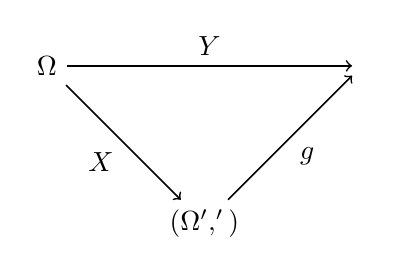
\begin{tikzpicture}
\node (Omega) at (0, 2) {$\Omega$};
\node (R1)		at (4, 2) {$\R$};
\node (R2)		at (2, 0) {$(\Omega', \sA')$};
\draw[->, semithick] (Omega) -- node[above]{$Y$} 				(R1);
\draw[->, semithick] (Omega) -- node[below left]{$X$}		(R2);
\draw[->, semithick] (R2)		 -- node[below right]{$g$}	(R1);
\end{tikzpicture}
	\end{center}
\end{enumerate}
Ist $X$ surjektiv, so folgt ferner, dass $g$ eindeutig ist.
\end{lemma}

\begin{beweis}
Die Richtung von \ref{Nummer1511A2} nach \ref{Nummer1511A1} ist trivial. F�r die andere Richtung f�hren wir wieder aufeinanderfolgende Schritte aus. Im ersten Schritt sei $Y = \ind_A$, dann ist $A \in \sigma(X)$, da $Y$ nach Voraussetzung $\sigma(X)$-messbar ist. Dann existiert ein $A' \in \sA'$ mit $A = X^{-1}(A')$ und wir setzen $g := \ind_{A'}$. F�r den zweiten Schritt sei $Y = \sum_{i=1}^n \alpha_i \ind_{A_i}$ und wir setzen $g := \sum_{i=1}^n \alpha_i\ind_{A_i'}$, wobei wie im ersten Schritt $X^{-1}(A_i') = A_i$ setzen.

Im dritten Schritt sei $Y \geq 0$, dann existiert eine Folge $Y_n \nearrow Y$ von Treppenfunktionen und mit Hilfe des zweiten Schritts existiert entsprechend eine Folge $g_n$ mit $Y_n = g_n \circ X$. Da die Konstruktion im zweiten Schritt monoton ist, folgt $g_n \nearrow g := \lim g_n$. Im letzten Schritt zerlegen wir schlie�lich wie gewohnt $Y = Y^+ - Y^-$ und erhalten so den Rest der Aussage.

Zu zeigen bleibt nun noch die Eindeutigkeit, wenn $X$ surjektiv ist. Sind $\omega_1, \omega_2 \in \Omega$ mit $X(\omega_1) = X(\omega_2)$, so gilt auch $Y(\omega_1) = g(X(\omega_1)) = g(X(\omega_2)) = Y(\omega_2)$. Sei nun $x \in \Omega'$, dann existiert ein $\omega \in \Omega$ mit $X(\omega) = x$. Dann erhalten wir $g(x) = g(X(\omega)) = Y(\omega)$ und $g$ ist eindeutig, wobei $Y(\omega)$ nach unseren Vor�berlegungen von der speziellen Wahl des $\omega$ unabh�ngig ist.
\end{beweis}

Wir wollen diese Ergebnisse nun wieder interpretieren. Dazu sei $A, B \in \sA$ und $X := \ind_B$, sowie $\sB := \sigma(X)$. Dann ist $\sB = \{\emptyset, B, B^c, \Omega\}$ und nach Lemma \ref{Nummer1.5.11} gilt $P(A~|~\ind_B) = P(A~|~\sB) = \E(\ind_A~|~\sB) = g \circ \ind_B$. F�r $\omega \in B$ folgt dann
\begin{align*}
P(B)P(A~|~\ind_B)(\omega) &= P(B)g(1) = \int g(1) \ind_B~\dd P = \int g \circ \ind_B~\dd P = \int_B \E(\ind_A~|~B)~\dd P = \int_B \ind_A~\dd P\\
													&= P(A \cap B)\text{.}
\end{align*}
Ist nun $P(B) > 0$, so folgt $P(A~|~\ind_B)(\omega) = P(A~|~B)$ f�r alle $\omega \in B$, aber wir wissen bereits, dass die linke Seite auch f�r $P(B)=0$ definiert ist.

\begin{definition}[Faktorisierter bedingter Erwartungswert]\label{Nummer1.5.12}
Es sei $(\Omega, \sA, P)$ ein Wahrscheinlichkeitsraum, $(\Omega', \sA')$ ein Messraum, $Y \in \sL_1(P)$ und $X\colon \Omega \to \Omega'$ messbar und surjektiv. Dann ist $\E(Y~|~X)$ $\sigma(X)$-messbar und mit Lemma \ref{Nummer1.5.11} existiert genau ein $g\colon \Omega' \to \R$ mit $\E(Y~|~X) = g \circ X$. F�r $x \in \Omega'$ schreiben wir dann $\E(Y~|~X = x) := g(x)$ und nennen $\E(Y~|~X = \cdot)$ den \deftxt{faktorisierten bedingten Erwartungswert}\index{bedingte Erwartung!faktorisierte}. Analog ist $P(A~|~X = x) = \E(\ind_A~|~X = x)$.
\end{definition}

F�r $A \in \sA$ ist $P(A~|~X = \cdot)$ nur bis auf $P_X$-Nullmengen eindeutig, da $\E(Y~|~X)$ nur bis auf $P$-Nullmengen bestimmt ist. F�r eine weitere Ausf�hrung verweisen wir auf \cite[Kap. 8.3, S. 182]{KLENKE}.
\chapter{Zeitdiskrete Martingale}

\begin{beschreibung}
Martingale waren urspr�nglich eine Klasse von Wettstrategien im 18. Jahrhundert Frankreichs, aber auch ein Begriff f�r bestimmte Pferdez�gel. In der Theorie der stochastischen Prozesse sind Martingale bestimmte Klassen von Prozessen, welche die stochastischen Prozesse gewisserma�en einschn�ren.
\end{beschreibung}

\section{Definition und einfache Beispiele}

Im Folgenden sei $(\Omega, \sA, P)$ immer ein Wahrscheinlichkeitsraum, sowie $T \subset [0, \infty)$ eine Indexmenge. Da wir vor allem zeitdiskrete Martingale betrachten werden, wird h�ufig $T = \N$ oder $T = \N_0$ sein.

\begin{definition}[Filtration]\label{Nummer2.1.1}
Eine Familie $\sF = (\sF_t)_{t \in T}$ von $\sigma$-Unteralgebren von $\sA$ hei�t \deftxt{Filtration}\index{Filtration} genau dann, wenn $\sF_s \subset \sF_t$ f�r alle $s, t \in T$ mit $s \leq t$ gilt.
\end{definition}

Wird $\sF_t$ als unser Kenntnisstand zum Zeitpunkt $t$ betrachtet, so sichert die Filtrationseigenschaft, dass wir h�chstens dazulernen, unser Kenntnisstand mit der Zeit also gr��er wird.

\begin{definition}[Adaptierter stochastischer Prozess]\label{Nummer2.1.2}
Sei $X = (X_t)_{t \in T}$ ein $\sX$-wertiger stochastischer Prozess und $\sF = (\sF_t)_{t \in T}$ eine Filtration, dann hei�t $X$ an $\sF$ \deftxt{adaptiert}\index{Stochastischer Prozess!adaptierter} genau dann, wenn $X_t$ f�r alle $t \in T$ $\sF_t$-messbar ist.
\end{definition}

Dies bedeutet also, dass $X_t$ mit unserem Kenntnisstand $\sF_t$ beschreibbar ist.

\begin{definition}[Vorhersagbarer stochastischer Prozess]\label{Nummer2.1.3}
Sei $X = (X_n)_{n \geq 0}$ ein $\sX$-wertiger stochastischer Prozess und $\sF = (\sF_n)_{n \geq 0}$ eine Filtration, dann hei�t $X$ \deftxt{vorhersagbar}\index{Stochastischer Prozess!vorhersagbarer} oder \deftxt{previsibel}\index{Stochastischer Prozess!previsibler} bez�glich $\sF$ genau dann, wenn $X_n$ f�r alle $n \geq 1$ $\sF_{n-1}$-messbar und $X_0$ konstant ist.
\end{definition}

In diesem Fall k�nnen wir den Prozess also bereits aus dem Kenntnisstand vom Zeitpunkt zuvor beschreiben und daher gewisserma�en vorhersagen. Ist $X$ previsibel, so ist $X$ auch adaptiert. Eine h�ufig verwendete Filtration ist die \deftxt{nat�rliche Filtration}\index{Filtration!nat�rliche}:\\
Ist $(X_t)_{t \in T}$ ein stochastischer Prozess und $\sF_t := \sigma\left(X_s : T \ni s \leq t\right)$, dann ist $X$ an $\sF := (\sF_t)_{t \in T}$ adaptiert. Dies ist die kleinste Filtration bez�glich welcher $X$ adaptiert ist. Oft werden wir hierf�r $\sF_t^X := \sF_t$ schreiben. Wir kommen nun zum eigentlichen Objekt unserer Begierde:

\begin{definition}[Martingal]\label{Nummer2.1.4}
Sei $M = (M_n)_{n \geq 0}$ ein $\R$-wertiger stochastischer Prozess mit $M_n \in \sL_1(P)$ f�r alle $n \geq 0$, sowie $\sF = (\sF_n)_{n \geq 0}$ eine Filtration, an welcher $M$ adaptiert ist. Dann hei�t $M$
\begin{enumerate}
	\item \deftxt{(zeitdiskretes) Martingal}\index{Martingal} bez�glich $\sF$ genau dann, wenn $\E(M_n~|~\sF_{n-1}) = M_{n-1}$ $P$-fast sicher f�r alle $n \geq 1$ gilt.
	\item \deftxt{Sub-Martingal}\index{Martingal!Sub-Martingal} genau dann, wenn $\E(M_n~|~\sF_{n-1}) \geq M_{n-1}$ $P$-fast sicher f�r alle $n \geq 1$ gilt.
	\item \deftxt{Super-Martingal}\index{Martingal!Super-Martingal} genau dann, wenn $\E(M_n~|~\sF_{n-1}) \leq M_{n-1}$ $P$-fast sicher f�r alle $n \geq 1$ gilt.
\end{enumerate}
\end{definition}

Wir wollen an dieser Stelle einige einfache Eigenschaften festhalten:
\begin{enumerate}
	\item Ist $M$ ein Martingal, so ist es nat�rlich auch ein Sub- und ein Super-Martingal.
	\item $M$ ist ein Sub-Martingal genau dann, wenn $-M$ ein Super-Martingal ist.
	\item Ist $M$ ein Martingal, so ist auch $(M_n - M_0)_{n \geq 0}$ ein Martingal.
	\item Ist $M$ ein Martingal, so gilt $\E M_n = \E(\E(M_n~|~\sF_{n-1})) = \E M_{n-1}$ f�r alle $n \geq 1$, die Erwartungswerte von Martingalen �ndern sich also nicht �ber die Zeit. F�r Sub-Martingale (Super-Martingale) gilt mit analoger Begr�ndung, dass die Erwartungswerte monoton steigen (fallen).
\end{enumerate}

Die beste Prognose von $M_n$ zum Zeitpunkt $n-1$ ist, wie wir im letzten Kapitel gesehen haben, $\E(M_n~|~\sF_{n-1})$. Die Martingaleigenschaft besagt nun gerade, dass die Prognose gleich $M_{n-1}$ ist.

Alternativ wollen wir Martingale nun als ein Spiel interpretieren: Es sei $M = (M_n)_{n \geq 0}$ ein $\R$-wertiger stochastischer Prozess, der an $(\sF_n)_{n \geq 0}$ adaptiert ist. Dabei soll $M_n$ unser Verm�gen zum Zeitpunkt $n$ beschreiben, also ist $M_n - M_{n-1}$ unser Gewinn in der $n$-ten Spielrunde. Ist $M$ ein Martingal, so gilt mit der Martingal- und Adaptionseigenschaft
\begin{align*}
\E(M_n - M_{n-1}~|~\sF_{n-1}) &= \E(M_n~|~\sF_{n-1}) - \E(M_{n-1}~|~\sF_{n-1}) = M_{n-1} - M_{n-1} = 0\text{.}
\end{align*}
In der $n$-ten Spielrunde ist das Spiel also fair, sofern unser Kenntnisstand zum Zeitpunkt $n - 1$ zugrundegelegt wird. Ist $M$ ein Super-Martingal, so folgt analog, dass $\E(M_{n-1} - M_n~|~\sF_{n-1}) \leq 0$ gilt, also ist das Spiel auf unsere Kosten unfair.

\begin{beispiel}[Summen unabh�ngiger Zufallsvariablen]\label{Nummer2.1.5}
Ist $(X_n)_{n \geq 0}$ eine Folge unabh�ngiger Zufallsvariablen mit $X_n \in \sL_1(P)$ f�r alle $n \geq 0$ und $X_0 = 0$. Dann ist
\begin{align*}
M_n &:= \sum_{i=0}^n (X_i - \E X_i) \qquad \text{f�r } n \geq 0
\end{align*}
ein Martingal bez�glich der nat�rlichen Filtration von $M_n$. Die Adaptionseigenschaft und Integrierbarkeit sind offensichtlich, zu zeigen bleibt die Martingaleigenschaft. Es ist
\begin{align*}
\E(M_{n+1} - M_n~|~\sF_n) &= \E(X_{n+1} - \E X_{n+1}~|~\sF_n) = \E(X_{n+1}~|~\sF_n) - \E X_{n+1} = \E X_{n+1} - \E X_{n+1} = 0\text{,}
\end{align*}
wobei wir ausgenutzt haben, dass $X_{n+1}$ und $\sF_n$ unabh�ngig sind.
\end{beispiel}

\begin{beispiel}[Martingal durch Filtration]\label{Nummer2.1.6}
Es sei $X \in \sL_1(P)$ und $(\sF_n)_{n \geq 0}$ eine Filtration. Dann definiert
\begin{align*}
M_n &:= \E(X~|~\sF_n) \qquad \text{f�r } n \geq 0
\end{align*}
ein Martingal. Auch hier sind die Adaptionseigenschaft und Integrierbarkeit klar, zu beweisen bleibt also wieder die Martingaleigenschaft. Wegen $\sF_{n-1} \subset \sF_n$ gilt
\begin{align*}
\E(M_n~|~\sF_{n-1}) &= \E(\E(X~|~\sF_n)~|~\sF_{n-1}) = \E(X~|~\sF_{n-1}) = M_{n-1}\text{.} \qedhere
\end{align*}
\end{beispiel}

\begin{beispiel}[Produkte unabh�ngiger Zufallsvariablen]\label{Nummer2.1.7}
Es sei $(X_n)_{n \geq 0}$ eine Folge unabh�ngiger Zufallsvariablen mit $\sL_1(P) \ni X_n \geq 0$ und $\E X_n = 1$ f�r alle $n \geq 0$. Wir setzen $M_0 := 0$, $\sF_0 := \{\emptyset, \Omega\}$ und dann $M_n := X_1 \cdot \ldots \cdot X_n$ und $\sF_n := \sigma(X_1, \ldots, X_n)$. Dann ist $M_n$ ein Martingal. Die Adaptionseigenschaft ist nach Konstruktion klar und die Integrierbarkeit folgt aus $X_1 \cdot \ldots \cdot X_n \in \sL_1(P)$. Wir zeigen nun noch die Martingaleigenschaft. Es gilt
\begin{align*}
\E(M_n~|~\sF_{n-1}) &= \E(M_{n-1} \cdot X_n~|~\sF_{n-1}) \stackrel{\text{\ref{Nummer1.5.8}}}{=} M_{n-1} \cdot\E(X_n~|~\sF_{n-1}) = M_{n-1} \cdot \E X_n = M_{n-1} \cdot 1\text{.} \qedhere
\end{align*}
\end{beispiel}

Nach diesen etwas einfacheren Beispielen wollen wir nun noch ein komplizierteres Beispiel diskutieren:

\begin{beispiel}[Diskretes stochastisches Integral]\label{Nummer2.1.8}
Es sei $(X_n)_{n \geq 0}$ ein $\sF = (\sF_n)_{n \geq 0}$-adaptierter stochastischer Prozess, sowie $(H_n)_{n \geq 1}$ ein $\sF$-vorhersagbarer stochastischer Prozess. Dann hei�t der Prozess $H.X$, der durch
\begin{align*}
(H.X)_n &:= X_0 + \sum_{m=1}^n H_m(X_m - X_{m-1}) \qquad\text{f�r } n \geq 0
\end{align*}
definiert ist, \deftxt{diskretes stochastisches Integral}\index{Diskretes stochastisches Integral}. Ist $X$ ein Martingal, so hei�t $H.X$ auch \deftxt{Martingaltransformierte}\index{Martingaltransformierte} von $X$.

Wir wollen nun erl�utern, woher diese Bezeichnung kommt. Dazu ben�tigen wir das \deftxt{Stieltjes-Integral}\index{Stieltjes-Integral}, das durch
\begin{align*}
\int_0^t h~\dd g(x) &:= \lim \sum_{k=1}^n h(t_{k-1}) \left(g(t_k) - g(t_{k-1})\right)
\end{align*}
definiert ist, wobei der Grenzwert des Rangs der Zerlegung $0 = t_0 < t_1 < \ldots < t_n = t$ gegen Null betrachtet wird, das hei�t die Zerlegung immer feiner gemacht wird. Dieser Grenzwert existiert, wenn $g$ hinreichend regul�r ist. Bei $H.X$ wird die Grenzwertbildung weggelassen und die Zerlegung von $[0, n]$ ist sehr speziell gew�hlt, n�mlich $t_m = m$. Dies motiviert die Bezeichnung "`diskretes Integral"' f�r $H.X$. Ferner w�hlen wir $g(t_k) = X_k(\omega)$, das hei�t wir integrieren bez�glich einer zuf�lligen Funktion, was die Bezeichnung "`stochastisches (Integral)"' motiviert. Man kann sp�ter den Grenzwert sogar durchf�hren, dazu ben�tigt man jedoch die Regularit�t der Trajektorien von $X$.
\end{beispiel}

\begin{lemma}\label{Nummer2.1.9}
Es sei $(X_n)_{n \geq 0}$ an eine Filtration $\sF$ adaptiert mit $X_i \in \sL_1(P)$ f�r alle $i \geq 0$. Ferner sei $(H_n)_{n \geq 1}$ vorhersagbar bez�glich $\sF$ mit $H_n(X_n - X_{n-1}) \in \sL_1$ f�r alle $n \geq 1$. Dann gilt:
\begin{enumerate}
	\item Ist $X$ ein Martingal, so ist auch $H.X$ ein Martingal.
	\item Ist $X$ ein Sub-/Super-Martingal und $H \geq 0$, so ist auch $H.X$ ein Sub-/Super-Martingal.
\end{enumerate}
\end{lemma}

\begin{beweis}
Wir beweisen beide Eigenschaften gleichzeitig. Es gilt
\begin{align*}
\E((H.X)_n - (H.X)_{n-1}~|~\sF_{n-1}) &= \E(H_n(X_n - X_{n-1})~|~\sF_{n-1}) \stackrel{\text{\ref{Nummer1.5.8}}}{=} H_n \cdot \E(X_n - X_{n-1}~|~\sF_{n-1})\\
\quad &= \begin{cases}0 & \text{falls $X$ Martingal}\\\geq 0 & \text{falls $X$ Sub-Martingal}\\\leq 0 & \text{falls $X$ Super-Martingal}\end{cases}\text{.}
\end{align*}
Damit ist alles gezeigt.
\end{beweis}
	\section{Grundlegende Eigenschaften}

In diesem Abschnitt wollen wir zwei Ziele erreichen. Zun�chst wollen wir einige M�glichkeiten kennenlernen, aus Martingalen neue Martingale zu konstruieren. Danach wollen wir zeigen, dass stochastische Prozesse im Wesentlichen aus Martingalen und vorhersagbaren stochastischen Prozessen bestehen.

\begin{satz}\label{Nummer2.2.1}
Es seien $X = (X_n)_{n \geq 0}$ und $Y = (Y_n)_{n \geq 0}$ reellwertige, $\sF$-adaptierte stochastische Prozesse, wobei $\sF$ eine Filtration ist. Dann gilt:
\begin{enumerate}
	\item\label{Nummer221A1} Sind $X$ und $Y$ Martingale und $\alpha, \beta \in \R$, so ist auch $\alpha X + \beta Y$ ein Martingal.
	\item\label{Nummer221A2} Sind $X$ und $Y$ beide Super- oder Sub-Martingale und $\alpha, \beta \geq 0$, so ist auch $\alpha X + \beta Y$ ein Super- bzw. Sub-Martingal.
	\item\label{Nummer221A3} Sind $X$ und $Y$ Super-Martingale, so ist $X \wedge Y := \min\{X, Y\}$ ebenfalls ein Super-Martingal. Sind $X$ und $Y$ Sub-Martingale, so ist analog $\max\{X, Y\}$ ein Sub-Martingal.
	\item\label{Nummer221A4} Ist $X$ ein Super-Martingal, $(T_n)_{n \geq 1} \subset \N$ mit $T_n \to \infty$ und $\E X_{T_n} \geq \E X_0$ f�r alle $n \geq 1$, so ist $X$ ein Martingal.
\end{enumerate}
\end{satz}

\begin{beweis}
Die ersten beiden Eigenschaften lassen sich durch simples Nachrechnen unter Verwendung der Linearit�t des bedingten Erwartungswertes beweisen. F�r \ref{Nummer221A3} setzen wir $Z_n := X_n \wedge Y_n$. Wegen $|Z_n| \leq |X_n| + |Y_n|$ folgt dann $Z_n \in \sL_1$ und die Tatsache, dass $Z_n$ adaptiert ist. Dann erhalten wir
\begin{align*}
\E(Z_n~|~\sF_{n-1}) &\leq \E(X_n~|~\sF_{n-1}) \leq \E(X_{n-1}~|~\sF_{n-1}) \leq \E(Y_{n-1}~|~\sF_{n-1}) \leq \E(Z_{n-1}~|~\sF_{n-1})\text{.}
\end{align*} 
Nun wollen wir \ref{Nummer221A4} beweisen. Dazu sei $m \in \N$, dann existiert ein $n \in \N$ mit $m < T_n$ und wir setzen $Y_i := \E(X_{T_n}~|~\sF_i)$ f�r $i < T_n$. Zuerst zeigen wir, dass $P$-fast sicher $X_i = Y_i$ f�r alle $i < T_n$ gilt. Dazu betrachte
\begin{align*}
Y_i &= \E(X_{T_n}~|~\sF_i) = \E(\E(X_{T_n}~|~\sF_{T_n - 1})~|~\sF_i)\\
		&\leq \E(X_{T_n-1}~|~\sF_i)\\
		&\phantom{\leq}\quad\vdots\\
		&\leq \E(X_i~|~\sF_i) = X_i\text{.}
\end{align*}
Mit dieser Rechnung gilt nun
\begin{align*}
\E X_0 &\leq \E X_{T_n} = \E(\E( X_{T_n}~|~\sF_i)) = \E Y_i\\
			 &\leq \E X_i = \E(\E(X_i~|~\sF_{i-1}))\\
			 &\leq \E X_{i-1}\\
			 &\phantom{\leq}\quad\vdots\\
			 &\leq \E X_0\text{.}
\end{align*}
Damit m�ssen all diese Ungleichungen also tats�chlich Gleichungen sein und wir erhalten insbesondere $\E X_i = \E Y_i$ f�r alle $i < T_n$. Fassen wir dies zusammen, so erhalten wir $X_i = Y_i$ $P$-fast sicher f�r alle $i < T_n$. Nun gilt
\begin{align*}
\E(X_m~|~\sF_{m-1}) &= \E(\underbrace{\E(X_{T_n}~|~\sF_m)}_{= Y_m}~|~\sF_{m-1}) = \E(X_{T_n}~|~\sF_{m-1}) = Y_{m-1} = X_{m-1}\text{.} \qedhere
\end{align*}
\end{beweis}

\begin{satz}\label{Nummer2.2.2}
Es sei $X = (X_n)_{n \geq 0}$ ein Martingal und $\phi\colon \R \to \R$ eine konvexe Abbildung. Dann gilt:
\begin{enumerate}
	\item\label{Nummer222A1} Falls f�r den positiven Anteil der Komposition $\E(\phi \circ X)^+ < \infty$ f�r alle $n \geq 0$ gilt, so folgt, dass $\phi \circ X$ ein Sub-Martingal ist.
	\item\label{Nummer222A2} Ist $X_n \in \sL_p$ f�r ein $p \in [1, \infty)$ und alle $n \geq 0$, so ist $|X|^p$ ein Sub-Martingal.
\end{enumerate}
\end{satz}

\begin{beweis}
Die Aussage \ref{Nummer222A2} folgt aus \ref{Nummer222A1} f�r $\phi(t) := |t|^p$. Beweisen wir also \ref{Nummer222A1}. Dazu sei $v(x) = ax+b$ affin linear f�r $x \in \R$ mit $v \leq \phi$ (vgl. Beweis von Satz \ref{Nummer1.5.5}). Dann gilt $\phi^- = \max\{0, -\phi\} \leq \max\{0, -v\} = v^-$ und wir erhalten
\begin{align*}
\E(\phi \circ X_n)^- &\leq \E(v \circ X)^- \leq |a| \E |X_n| + |b| < \infty\text{.}
\end{align*}
Dann ist $\phi \circ X_n \in \sL_1$. Nun folgt mit Satz \ref{Nummer1.5.5}
\begin{align*}
\E(\phi \circ X_n~|~\sF_{n-1}) &\geq \phi \E(X_n~|~\sF_{n-1}) = \phi \circ X_{n-1}\text{.} \qedhere
\end{align*}
\end{beweis}

\begin{lemma}\label{Nummer2.2.3}
Es sei $M = (M_n)_{n \geq 0}$ ein $\sF$-adaptiertes, vorhersagbares Martingal. Dann gilt $P$-fast sicher $M_n = M_0$ f�r alle $n \geq 0$.
\end{lemma}

\begin{beweis}
Es gen�gt, induktiv zu zeigen, dass $P$-fast sicher $M_n = M_{n-1}$ f�r alle $n \geq 1$ gilt. Dies gilt aber wegen $M_n = \E(M_n~|~\sF_{n-1}) = M_{n-1}$.
\end{beweis}

\begin{lemma}\label{Nummer2.2.4}
Es sei $M = (M_n)_{n \geq 0}$ ein Martingal, dann folgt $\E(M_n \cdot M_m) = \E M_m^2$ f�r alle $0 \leq m \leq n$.
\end{lemma}

\begin{beweis}
Wir k�nnen ohne Einschr�nkung $n > m$ annehmen, da der Fall $n = m$ trivial ist. Dann gilt mit iterierter Anwendung der Martingaleigenschaft
\begin{align*}
\E(M_n \cdot M_m) &= \E(\E(M_n \cdot M_m ~|~ \sF_m)) = \E(M_m(\underbrace{\E(M_n~|~\sF_m)}_{= M_m})) = \E(M_m \cdot M_m)\text{.} \qedhere
\end{align*}
\end{beweis}

\begin{satz}[Doob-Zerlegung]\index{Doob!-Zerlegung}\label{Nummer2.2.5}
Es sei $X = (X_n)_{n \geq 0}$ ein an $\sF = (\sF_n)_{n \geq 0}$ adaptierter stochastischer Prozess mit $X_n \in \sL_1(P)$ f�r alle $n \geq 0$. Dann existiert -- bis auf Ununterscheidbarkeit -- genau ein Martingal $M$ und ein $\sF$-vorhersagbarer stochastischer Prozess $A$ mit $A_0 = 0$, so dass $X = M + A$ gilt. Ferner ist $X$ ein Sub-Martingal genau dann, wenn $A$ monoton wachsend ist.
\end{satz}

Mit anderen Worten bestehen stochastische Prozesse also aus Martingalen und vorhersagbaren Prozessen.

\begin{beweis}
Wir zeigen zun�chst die Existenz. F�r $n \geq 0$ sei dazu
\begin{align*}
M_n &:= X_0 + \sum_{k=1}^n \left(X_k - \E(X_k~|~\sF_{k-1})\right)\text{,}
\shortintertext{sowie}
A_n &:= -\sum_{k=1}^n \left(X_{k-1} - \E(X_k~|~\sF_{k-1})\right)\text{.}
\end{align*}
Dann gilt, dass $A_n$ nach Konstruktion $\sF_{n-1}$-messbar ist, da es als Summe �ber $\sF_{k-1}$-messbare Terme entsteht und $\sF_{k-1} \subset \sF_{n-1}$ f�r $k \in \{1, \ldots, n\}$ gilt. Dann folgt, dass $A$ $\sF$-vorhersagbar ist; dass $A_0 = 0$ gilt ist klar. Ferner ist $M_n$ nach Konstruktion mit analoger Argumentation $\sF_n$-messbar und integrierbar, wir m�ssen also noch die Martingaleigenschaft zeigen. Dazu betrachten wir
\begin{align*}
\E(M_n - M_{n-1}~|~\sF_{n-1}) &= \E(X_n - \E(X_n~|~\sF_{n-1})~|~\sF_{n-1}) = \E(X_n~|~\sF_{n-1}) - \E(X_n~|~\sF_{n-1}) = 0\text{.}
\end{align*}
Nun bleibt noch zu zeigen, dass $M$ und $A$ tats�chlich $X$ zerlegen. Dies gilt wegen
\begin{align*}
M_n + A_n &= X_0 + \sum_{k=1}^n (X_k - \E(X_k~|~\sF_{k-1})) - \sum_{k=1}^n X_{k-1} + \sum_{k=1}^n \E(X_k~|~\sF_{k-1})\\
					&= X_n\text{.}
\end{align*}
Damit ist die Existenz gezeigt und wir zeigen die Eindeutigkeit. Dazu sei $X = M + A = M' + A'$, dann gilt $M - M' = A' - A$. Nach Satz \ref{Nummer2.2.1} ist $M - M'$ ein Martingal und $A' - A$ ist vorhersagbar, also auch $M - M'$. Mit Lemma \ref{Nummer2.2.3} folgt dann $M_n - M_n' = M_0 - M_0' = A_0 - A_0' = 0 - 0 = 0$, also folgt $P$-fast sicher $M = M'$.

Zum Schluss beweisen wir noch, dass $X$ ein Sub-Martingal ist genau dann, wenn $A$ wachsend ist. Dazu �berlegen wir uns zun�chst
\begin{align*}
\E(X_n~|~\sF_{n-1}) &= \E(M_n~|~\sF_{n-1}) + \E(A_n~|~\sF_{n-1}) = M_{n-1} + A_n\text{.}
\end{align*}
Also ist $X$ ein Sub-Martingal. Daraus folgt $M_{n-1} + A_n = \E(X_n~|~\sF_{n-1}) \geq X_{n-1} = M_{n-1} + A_{n-1}$ und wir erhalten $A_n \geq A_{n-1}$. Die andere Richtung folgt analog.
\end{beweis}

\begin{korollar}\label{Nummer2.2.6}
Es sei $X = (X_n)_{n \geq 0}$ ein quadrat-integrierbares $\sF$-Martingal, d.\,h. es gilt $X_n \in \sL_2$ f�r alle $n \geq 0$. Dann gilt:
\begin{enumerate}
	\item\label{Nummer226A1} $X^2$ ist ein Sub-Martingal.
	\item\label{Nummer226A2} Es gibt genau einen $\sF$-vorhersagbaren stochastischen Prozess $A$ mit $A_0 = 0$, so dass $X^2-A$ ein Martingal ist. Dieser Prozess $A$ hei�t \deftxt{quadratischer Variationsprozess}\index{Quadratischer Variationsprozess} von $X$ und wird mit $\langle X \rangle := A$ bezeichnet.
	\item\label{Nummer226A3} Der Prozess $\langle X \rangle$ ist monoton wachsend.
	\item\label{Nummer226A4} Es gilt $\displaystyle\langle X \rangle_n = \sum_{i=1}^n \E((X_i - X_{i-1})^2~|~\sF_{i-1})$ und $\displaystyle \E\langle X \rangle_n = \Var (X_n - X_0)$.
\end{enumerate}
\end{korollar}

\begin{beweis}
Aussage \ref{Nummer226A1} folgt unmittelbar aus Satz \ref{Nummer2.2.2}. Aussage \ref{Nummer226A2} folgt aus Satz \ref{Nummer2.2.5}, denn f�r $X^2$ mit $X^2 = M + A$ erhalten wir $X^2 - A = M$. Aussage \ref{Nummer226A3} folgt ebenfalls aus Satz \ref{Nummer2.2.5}. Wir zeigen also noch \ref{Nummer226A4}. Dazu betrachten wir
\begin{align*}
\sum_{i=1}^n \E((X_i - X_{i-1})^2~|~\sF_{i-1}) &= \sum_{i=1}^n \E(X_i^2 - 2X_iX_{i-1} + X_{i-1}^2~|~\sF_{i-1})\text{,}
\shortintertext{durch Auseinanderziehen und Anwenden der Definitionen der bedingten Erwartung und Martingalen erhalten wir dann}
\quad &= \sum_{i=1}^n \left(\E(X_i^2~|~\sF_{i-1}) - X_{i-1}^2\right) \stackrel{\text{\ref{Nummer2.2.5}}}{=} A_n\\
\quad &= \langle X \rangle_n\text{.}
\end{align*}
Nun wollen wir noch die Formel f�r den Erwartungswert beweisen. Es gilt
\begin{align*}
\E A_n &= \sum_{i=1}^n \E(\E(X_i - X_{i-1})^2~|~\sF_{i-1}) = \sum_{i=1}^n \E\left(X_i^2 - 2X_iX_{i-1} + X_{i-1}^2\right)\text{,}
\shortintertext{und wieder durch Auseinanderziehen und Lemma \ref{Nummer2.2.4} erhalten wir}
\quad &= \sum_{i=1}^n \left(\E X_i^2 - \E X_{i-1}^2\right) = \E X_n^2 - \E X_0^2 = \E X_n^2 - 2\E X_nX_0 + \E X_0^2 = \E (X_n - X_0)^2\\
\quad &= \Var (X_n - X_0)\text{,}
\end{align*}
da $\E X_n = \E X_0$ gilt, wie wir bereits gesehen haben.
\end{beweis}

\begin{beispiel}\label{Nummer2.2.7}
Es seien $(Y_i)_{i \geq 1}$ unabh�ngig mit $Y_i \in \sL_2(P)$ und $\E Y_i = 0$ f�r alle $i \geq 0$, sowie $X_n := \sum_{i=1}^n Y_i$ f�r $n \geq 0$. Dann gilt
\begin{align*}
\langle X \rangle_n &= \sum_{i=1}^n \E Y_i^2 = \sum_{i=1}^n \Var Y_i\text{.} \qedhere
\end{align*}
\end{beispiel}

\begin{beispiel}\label{Nummer2.2.8}
Es seien $(Y_i)_{i \geq 0}$ unabh�ngig mit $Y_i \in \sL_2(P)$ und $\E Y_i = 1$ f�r alle $i \geq 0$, sowie $X_n := \prod_{i=1}^n Y_i$ f�r $n \geq 0$. Dann gilt
\begin{align*}
\langle X \rangle_n &= \sum_{i=1}^n X_{i-1}^2 \Var Y_i\text{.} \qedhere
\end{align*}
\end{beispiel}
	\section{Stoppzeiten}

Wir w�rden stochastische Prozesse gerne in Abh�ngigkeit ihres Verhaltens bis zum Eintritt eines bestimmten Ereignisses untersuchen beziehungsweise modifizieren. Dazu sei $(\Omega, \sA, P)$ wie �blich ein Wahrscheinlichkeitsraum.

\begin{definition}[Stoppzeit]\label{Nummer2.3.1}
Es sei $\sF = (\sF_n)_{n \geq 0}$ eine Filtration. Eine Abbildung $\tau\colon \Omega \to \overline{\N_0} := \N_0 \cup \{\infty\}$ hei�t \deftxt{Stoppzeit}\index{Stoppzeit} genau dann, wenn
\begin{align*}
\{\tau \leq n\} \in \sF_n \qquad \text{f�r alle } n \geq 0\text{.}
\end{align*}
\end{definition}

Falls wir einen stochastischen Prozess bei der Zeit $\tau(\omega)$ in Abh�ngigkeit des Verhaltens bis zur Zeit $\tau(\omega)$ anhalten wollen -- wir werden darauf gleich noch n�her eingehen --, so darf $\tau(\omega)$ nur von unserem Kenntnisstand bis zur Zeit $\tau(\omega)$ abh�ngen. Die Menge $\{\tau \leq n\}$ enth�lt alle Zeiten vor dem Zeitpunkt $n$, die nur von der Kenntnis bis zu diesem Zeitpunkt abh�ngen. 

\begin{information}
F�r zeitdiskrete stochastische Prozesse -- auf die wir uns hier ja im Wesentlichen beschr�nken --, kann man statt der in Definition \ref{Nummer2.3.1} verwendeten Menge auch $\{\tau = n\}$ verwenden.
\end{information}

\begin{beispiel}[Eintrittszeit]\label{Nummer2.3.2}
Es sei $(X_n)_{n \geq 0}$ ein $\sF$-adaptierter Prozess und $A \subset \R$ messbar. Dann ist die \deftxt{Eintrittszeit}\index{Eintrittszeit} $\tau_A\colon \Omega \to \overline{\N_0}$ mit $\omega \mapsto \inf\{n \in \N_0 : X_n(\omega) \in A\}$ eine Stoppzeit, d.\,h. $\tau_A(\omega)$ ist der erste Zeitpunkt, zu welchem die Trajektorie $X(\omega)$ in $A$ liegt. Betrachte hierzu
\begin{align*}
\{\tau_A \leq n\} &= \{\omega : \exists_{k \in \{0, \ldots, n\}} : X_k(\omega) \in A\} = \bigcup_{k=0}^n \{X_k \in A\} \in \sF_n\text{.} \qedhere
\end{align*}
\end{beispiel}

\begin{beispiel}[Konstante Stoppzeit]\label{Nummer2.3.3}
Es sei $\sF$ eine Filtration und $n_0 \in \N_0$. Dann ist $\tau\colon \Omega \to \overline{\N_0}$ mit $\omega \mapsto n_0$ eine (\deftxt{konstante}\index{Stoppzeit!konstante}) Stoppzeit. Betrachte
\begin{align*}
\{\tau \leq n\} &= \begin{cases}\emptyset & \text{falls } n < n_0\\\Omega & \text{falls } n \geq n_0\end{cases} \in \sF_n\text{.} \qedhere
\end{align*}
\end{beispiel}

\begin{lemma}\label{Nummer2.3.4}
Seien $\sigma$ und $\tau$ Stoppzeiten, dann gilt
\begin{enumerate}
	\item\label{Nummer234A1} $\sigma \wedge \tau := \min\{\sigma, \tau\}$ und $\sigma \vee \tau := \max\{\sigma, \tau\}$ sind Stoppzeiten.
	\item\label{Nummer234A2} $\sigma + \tau$ ist eine Stoppzeit.
	\item\label{Nummer234A3} $\tau + s$ ist f�r alle $s \geq 0$ eine Stoppzeit.
\end{enumerate}
\end{lemma}

Insbesondere gilt zu beachten, dass die Bedingung $s \geq 0$ in Aussage \ref{Nummer234A3} des Lemmas essentiell ist und die Aussage f�r $s < 0$ im Allgemeinen nicht gilt.

\begin{beweis}
F�r \ref{Nummer234A1} betrachten wir $\{\tau \vee \sigma \leq n\} = \{\tau \leq n\} \cap \{\sigma \leq n\}$ und $\{\tau \wedge \sigma \leq n\} = \{\tau \leq n\} \cup \{\sigma \leq n\}$, diese Mengen sind offenbar messbar. 

F�r \ref{Nummer234A2} sei $n \in \N_0$, dann folgt aus \ref{Nummer234A1}, dass $\tau \vee n$ und $\tau \wedge n$ Stoppzeiten sind. F�r $m < n$ gilt nun $\{\tau \wedge n \leq m\} \in \sF_m \subset \sF_n$, f�r $m \geq n$ gilt $\{\tau \wedge n \leq m\} = \Omega \in \sF_n$. Damit ist $\tau' := (\tau \wedge n) + \ind_{\{\tau > n\}}$ eine $\sF_n$-messbare Zufallsvariable. Analog erhalten wir die $\sF_n$-Messbarkeit von $\sigma' := (\sigma \wedge n) + \ind_{\{\sigma > n\}}$. Damit folgt $\tau' + \sigma' \in \sF_n$. Schlie�lich gilt f�r $\tau \leq n$ und $\sigma \leq n$, dass $\tau' + \sigma' = \tau + \sigma$ gilt, ist aber zum Beispiel $\tau > n$, so ist $\tau' = n+1 > n$. Damit folgt $\{\sigma + \tau \leq n\} = \{\sigma' + \tau' \leq n\} \in \sF_n$.

Aussage \ref{Nummer234A3} folgt aus Aussage \ref{Nummer234A2} und Beispiel \ref{Nummer2.3.3}. Wir wollen noch zeigen, warum die Aussage f�r $s < 0$ nicht stimmt. Es ist $\{\tau + s \leq n\} = \{\tau \leq n-s\} \in \sF_{n-s}$, aber im Allgemeinen gilt $\sF_{n-s} \not\subset \sF_n$. 
\end{beweis}

\begin{definition}[Gestoppter stochastischer Prozess]\label{Nummer2.3.5}
Sei $\tau$ eine endliche Stoppzeit (d.\,h. $\tau < \infty$ $P$-fast sicher) und $X = (X_n)_{n \geq 0}$ ein $\sF$-adaptierter stochastischer Prozess. Wir definieren:
\begin{enumerate}
	\item Es sei $X_\tau\colon \Omega \to \R$ eine Abbildung verm�ge $\omega \mapsto X_{\tau(\omega)}(\omega)$. Dies ist der Wert der Trajektorie $X(\omega)$ zum Stoppzeitpunkt $\tau(\omega)$.
	\item \deftxt{Gestoppter Prozess}\index{Stochastischer Prozess!gestoppter}: $X^\tau = (X_n^\tau)_{n \geq 0}$ sei definiert durch
	\begin{align*}
	X_n^\tau &:= X_{\tau \wedge n} = \begin{cases}X_n & \text{f�r } n \leq \tau\\ X_\tau & \text{f�r } n \geq \tau\end{cases}\text{.}
	\end{align*}
\end{enumerate}
\end{definition}

Die f�r die stochastischen Prozesse typische Frage ist nun, in welchem Sinne $X_\tau$ und $X^\tau$ messbar sind, von welchen Kenntnisst�nden diese Variablen also abh�ngen. Dies wollen wir nun diskutieren.

\begin{definition}[$\tau$-Vergangenheit]\label{Nummer2.3.6}
Es sei $(\Omega, \sA, P)$ ein Wahrscheinlichkeitsraum, $\sF = (\sF_n)_{n \geq 0}$ eine Filtration und $\tau$ eine $\sF$-Stoppzeit. Dann ist
\begin{align*}
\sF_\tau &:= \{A \in \sA : A \cap \{\tau \leq n\} \in \sF_n \text{ f�r alle } n \geq 0\}
\end{align*}
eine $\sigma$-Algebra. Diese wird die \deftxt{$\sigma$-Algebra der $\tau$-Vergangenheit}\index{$\tau$-Vergangenheit} genannt.
\end{definition}

\begin{lemma}\label{Nummer2.3.7}
Es seien $\sigma$ und $\tau$ Stoppzeiten. Dann gelten die folgenden Aussagen:
\begin{enumerate}
	\item\label{Nummer237A1} Gilt $\sigma \leq \tau$, so folgt $\sF_\sigma \subset \sF_\tau$. 
	\item\label{Nummer237A2} F�r $n \geq 0$ gilt $\sF_{\tau \wedge n} \subset \sF_n$.
\end{enumerate}
\end{lemma}

\begin{beweis}
Aussage \ref{Nummer237A2} folgt aus \ref{Nummer237A1}, da $\sigma := \tau \wedge n$ eine Stoppzeit mit $\sigma \leq \tau$ ist. Wir beweisen nun also \ref{Nummer237A1}. Sei $A \in \sF_\sigma$ und $n \geq 0$, dann gilt wegen $\{\tau \leq n\} \subset \{\sigma \leq n\}$
\begin{align*}
A \cap \{\tau \leq n\} &= \underbrace{A \cap \{\sigma \leq n\}}_{\in \sF_n} \cap \underbrace{\{\tau \leq n\}}_{\in \sF_n} \in \sF_n\text{,}
\end{align*}
also ist $A \in \sF_\tau$.
\end{beweis}

\begin{satz}[Messbarkeit von $X_\tau$ und $X^\tau$]\label{Nummer2.3.8}
Sei $X = (X_n)_{n \geq 0}$ ein $\sF$-adaptierter stochastischer Prozess und $\tau$ eine endliche Stoppzeit. Dann gilt:
\begin{enumerate}
	\item\label{Nummer238A1} $X_\tau$ ist $\sF_\tau$-messbar.
	\item\label{Nummer238A2} $X^\tau$ ist $\sF$-adaptiert und auch $\sF^\tau$-adaptiert, wobei $\sF^\tau_n := \sF_{\tau \wedge n}$ ist.
\end{enumerate}
\end{satz}

\begin{beweis}
Wir beweisen zun�chst \ref{Nummer238A1}. Sei $B \subset \R$ messbar. Dann m�ssen wir $\{X_\tau \in B\} \in \sF_\tau$, also $\{X_\tau \in B\} \cap \{\tau \leq n\} \in \sF_n$ f�r alle $n \geq 0$ zeigen. Dies geschieht �ber den folgenden, typischen Ansatz:
\begin{align*}
\{X_\tau \in B\} \cap \{\tau \leq n\} &= \{X_\tau \in B\} \cap \bigcup_{k=0}^n \{\tau = k\} = \bigcup_{k=0}^n \left(\{X_\tau \in B\} \cap \{\tau = k\}\right)\\
\quad &= \bigcup_{k=0}^n \{X_k \in B\} \in \sF_n\text{.}
\end{align*}
Kommen wir zu \ref{Nummer238A2}. Da $\tau \wedge n$ eine Stoppzeit ist, ist $X_n^\tau = X_{\tau \wedge n}$ nach \ref{Nummer238A1} $\sF_{\tau \wedge n}$-messbar und nach Lemma \ref{Nummer2.3.7} damit auch $\sF_n$-messbar.
\end{beweis}
	\section{Optional Stopping Theorem}

Sei $X$ ein Martingal und $\tau$ eine Stoppzeit. Die Kernaussage wird dann im Wesentlichen sein, dass $X^\tau$ ein Martingal ist.

\begin{satz}[Optional Stopping Theorem (Doob)]\index{Doob!Optional Stopping Theorem}\index{Optional Stopping Theorem}\label{Nummer2.4.1}
Sei $X = (X_n)_{n \geq 0}$ ein $\sF$-adaptierter stochastischer Prozess und $\tau$ eine endliche $\sF$-Stoppzeit. Dann gilt:
\begin{enumerate}
	\item\label{Nummer241A1} Ist $X$ ein (Super-/Sub-)Martingal, so ist auch $X^\tau$ ein (Super-/Sub-)Martingal.
	\item\label{Nummer241A2} Ist $X$ ein Martingal, so gilt $\E X_{\tau \wedge n} = \E X_0$ f�r alle $n \geq 0$. Ist $\tau$ $P$-fast sicher beschr�nkt, so gilt ferner $\E X_\tau = \E X_0$.
	\item\label{Nummer241A3} Aussage \ref{Nummer241A2} gilt auch analog f�r Super-/Sub-Martingale.
\end{enumerate}
\end{satz}

\begin{beweis}
Wir beweisen zun�chst \ref{Nummer241A1}. Dazu definieren wir $H := (H_n)_{n \geq 1}$ durch $H_n := \ind_{\{\tau \geq n\}} = 1 - \ind_{\{\tau < n\}} \in \sF_{n-1}$, also ist $H$ vorhersagbar. Au�erdem gilt $0 \leq H_n \leq 1$ f�r alle $n \geq 1$, also ist $H_n \cdot (X_n - X_{n-1}) \in \sL_1$. Mit Lemma \ref{Nummer2.1.9} folgt dann, dass $H.X$ ein Martingal ist. Wir m�ssen noch $H.X = X^\tau$ zeigen. Dazu w�hlen wir $n \geq 0$, dann gilt
\begin{align*}
(H.X)_n &= X_0 + \sum_{k=1}^n H_k(X_k - X_{k-1}) = X_0 + \sum_{k=1}^n \ind_{\{\tau \geq k\}} \cdot (X_k - X_{k-1})\\
\quad &= X_0 + \sum_{k=1}^{\tau \wedge n} (X_k - X_{k-1}) = X_{\tau \wedge n} = X_n^\tau\text{.} 
\end{align*}
F�r Super-/Sub-Martingale geht dies analog. Wir kommen nun zu \ref{Nummer241A2}. Da $X^\tau$ ein Martingal ist, folgt $\E X_{\tau \wedge n} = \E X_n^\tau = \E X_0^\tau = \E X_{\tau \wedge 0} = \E X_0$. F�r den zweiten Teil der Aussage sei $\tau$ nun $P$-fast sicher beschr�nkt, dann gilt $\tau \wedge n \to \tau$ $P$-fast sicher f�r $n \to \infty$. Sei nun $N \in \N_0$ mit $\tau \leq N$, dann ist $h = \max_{k = 0, \ldots, N} |X_k| \in \sL_1$ und $|X_{\tau \wedge n}| \leq h$ f�r alle $n \geq 0$. Mit dem Satz zur majorisierten Konvergenz folgt dann $\E X_{\tau \wedge n} = \E X_0 \to \E X_\tau$, also gilt $\E X_\tau = \E X_0$. All dies l�sst sich analog f�r Super-/Sub-Martingale zeigen.
\end{beweis}

\begin{beispiel}[Symmetrische Irrfahrt]\label{Nummer2.4.2}\index{Irrfahrt!symmetrische}
Seien $(Y_i)_{i \geq 1}$ i.\,i.\,d. Zufallsvariablen mit $P(Y_i = 1) = P(Y_i = -1) = \frac12$ und $X_n := \sum_{i=1}^n Y_i$ f�r $n \geq 0$. Ferner seien $a < 0$ und $b > 0$. Dann betrachten wir die Stoppzeiten
\begin{align*}
\tau_a &:= \inf\{n \geq 0 : X_n = a\}\text{,}\\
\tau_b &:= \inf\{n \geq 0 : X_n = b\}\text{,}\\
\tau_{a,b} &:= \tau_a \wedge \tau_b = \tau_{(-\infty, a] \cup [b, \infty)}\text{.}
\end{align*}
Zun�chst m�chten wir dies als ein faires Wettspiel interpretieren. Spieler 1 hat das Kapital $-a > 0$, Spieler 2 das Kapital $b > 0$. Dann gibt $Y_i = 1$ an, dass Spieler 1 gewinnt und eine Geldeinheit von Spieler 2 erh�lt. Die Stoppzeit $\tau_{a,b}$ gibt dann die Spieldauer bis zum Bankrott einer der Spieler an. Die Menge $A = \{\tau_{a,b} = \tau_a\}$ beschreibt also das Ereignis, dass Spieler 1 verliert, dass der Prozess $X$ also zuerst in $a$ (und nicht in $b$) ankommt. Wir wollen nun $P(A)$ und die mittlere Spieldauer $\E \tau_{a,b}$ bestimmen. 

Unser erstes Ziel ist es, $P(\tau < \infty) = 1$ f�r $\tau := \tau_{a,b}$ zu zeigen. Dies bedeutet, dass das Spiel $P$-fast sicher irgendwann endet. Dazu setzen wir $c := b-a$ und $A_k := \bigcap_{i=(k-1)c+1}^{kc} \{Y_i = 1\}$. Tritt $A_k$ ein, so ist das Spiel sp�testens zum Zeitpunkt $kc$ beendet, da Spieler 2 pleite ist. Es gilt $A_k \subset \{\tau \leq kc\}$ und daraus folgt $\bigcup_{k=1}^n A_k \subset \{\tau \leq nc\}$. Ferner ist $(A_k)_k$ eine unabh�ngige Familie und es gilt $P(A_k) = \left(\frac12\right)^c$. Damit erhalten wir
\begin{align*}
P(\tau = \infty) &= \lim_{n \to \infty} P(\tau > nc) \leq \lim_{n \to \infty} P\left(\bigcap_{k=1}^n A_k^C\right) = \lim_{n \to \infty} \prod_{k=1}^n P(A_k^C) = \lim_{n \to \infty} \left(1 - \left(\frac12\right)^c\right)^n\\
\quad &= 0\text{.}
\end{align*} 
Als n�chstes wollen wir nun $P(A)$ bestimmen. Klar ist, dass $\tau_{a,b} \wedge n \to \tau_{a,b} =: \tau$ $P$-fast sicher f�r $n \to \infty$, $X_n^\tau = X_{\tau \wedge n} \to X_\tau$ $P$-fast sicher und $\norm{X_n^\tau}_\infty = \norm{X_{\tau \wedge n}}_\infty \leq \max\{|a|,|b|\}$ gilt. Mit dem Satz zur majorisierten Konvergenz folgt dann $\E X_{\tau \wedge n} \to \E X_\tau$. Satz \ref{Nummer2.4.1} sagt nun, dass $\E X_n^\tau = \E X_0^\tau = 0$ gilt und mit obiger �berlegung erhalten wir $\E X_\tau = 0$. Damit folgt
\begin{align*}
0 &= \E X_\tau = a P(\tau_{a,b} = \tau_a) + b P(\tau_{a,b} = \tau_b) = a P(A) + b (1 - P(A))\text{.}
\end{align*}
Durch Aufl�sen der Gleichung erhalten wir $P(A) = \frac{b}{b-a}$. 

Das dritte Ziel ist die Berechnung der mittleren Spieldauer $\E \tau_{a,b}$. Da $X_n \in \sL_2$ f�r alle $n \geq 0$ gilt, existiert der quadratische Variationsprozess\footnote{Diesen haben wir in Korollar \ref{Nummer2.2.6} kennengelernt.} $\langle X \rangle$ und es gilt $\langle X \rangle_n = \sum_{i=1}^n \E Y_i^2 = n$ f�r alle $n \geq 0$. Nach Korollar \ref{Nummer2.2.6} ist $Z = X^2 - \langle X \rangle$ ein Martingal mit $Z_n = X_n^2 - n$. Mit Satz \ref{Nummer2.4.1} folgt nun
\begin{align*}
0 &= \E Z_0 = \E Z_n^\tau = \E (\underbrace{X_{\tau \wedge n}^2}_{\to X_\tau^2} - \underbrace{(\tau \wedge n)}_{\to \tau}) \to \E X_\tau^2 - \E\tau\text{,}
\end{align*}
woraus wir $0 = \E X_\tau^2 - \E\tau$ erhalten. Dann ist
\begin{align*}
\E \tau &= \E X_\tau^2 = a^2 P(A) + b^2 (1-P(A)) = -ab\text{.} \qedhere
\end{align*}
\end{beispiel}

\begin{satz}[Optional Sampling Theorem I]\label{Nummer2.4.3}\index{Optional Sampling Theorem}
Sei $X = (X_n)_{n \geq 0}$ ein $\sF$-Martingal und $\sigma \leq \tau$ seien $\sF$-Stoppzeiten. Ist $\tau$ beschr�nkt, so folgt
\begin{align*}
\E(X_\tau~|~\sF_{\sigma}) &= X_\sigma\text{.}
\end{align*}
\end{satz}

Ist $(\tau_n)_{n \geq 0}$ eine aufsteigende Folge beschr�nkter Stoppzeiten, so ist $(X_{\tau_n})_{n \geq 0}$ ein $(\sF_{\tau_n})_{n \geq 0}$-Martingal. Dabei ist $(\sF_{\tau_n})_{n \geq 0}$ nach Lemma \ref{Nummer2.3.7} eine Filtration und $X_{\tau_n}$ ist nach Satz \ref{Nummer2.3.8} $\sF_{\tau_n}$-messbar. Die Martingaleigenschaft liefert dann Satz \ref{Nummer2.4.3}.

\begin{beweis}
Es gelte $P$-fast sicher $\tau \leq N$. Dann ist $X_\tau$ integrierbar, da $|X_\tau| \leq \max_{n \leq N} |X_n|$ und $X_n \in \sL_1$ gilt. Zun�chst wollen wir $\E (X_N~|~\sF_\tau) = X_\tau$ $P$-fast sicher zeigen. Dazu sei $A \in \sF_\tau$, d.\,h. $A \cap \{\tau = k\} \in \sF_k$ f�r alle $k \geq 0$. Dann ist
\begin{align*}
\E (X_N \cdot \ind_A) &= \sum_{k=0}^N \E X_N\ind_A\ind_{\{\tau=k\}} = \sum_{k=0}^N \E X_N \ind_{A \cap \{\tau=k\}} = \sum_{k=0}^N \E(\ind_{A \cap \{\tau=k\}}\E(X_N~|~\sF_k))\\
\quad &= \sum_{k=0}^N \E(\ind_{A \cap \{\tau=k\}} X_k) = \sum_{k=0}^N \E X_\tau \ind_A \ind_{\{\tau=k\}}\\
\quad &= \E X_\tau \ind_A\text{.}
\end{align*}
Dadurch erhalten wir gerade die Gleichung, die wir beweisen wollten. Nun nutzen wir dies f�r den Beweis des Satzes. Es gilt $\sigma \leq \tau \leq N$ und mit Satz \ref{Nummer2.3.7} erhalten wir damit $\sF_\sigma \subset \sF_\tau$. Dann folgt
\begin{align*}
\E(X_\tau\mid\sF_\sigma) &= \E(\E(X_N\mid\sF_\tau)~|~\sF_\sigma) = \E(X_N\mid\sF_\sigma) = X_\sigma\text{.} \qedhere
\end{align*}
\end{beweis}
	\section{Konvergenzs�tze f�r Martingale I}

In diesem Abschnitt wollen wir untersuchen, ob ein $X$ existiert, so dass $X_n \to X$ gilt, falls $X_n$ ein (Super-/Sub-)Martingal ist.

Wir wollen f�r das kommende Lemma \ref{Nummer2.5.1} einen Ansatz diskutieren. Dazu sei $(x_n) \subset \R$ eine Folge, die weder eigentlich noch uneigentlich konvergiert. Dann ist $\liminf x_n < \limsup x_n$ und es seien $a < b$ mit $\liminf x_n < a < b < \limsup x_n$. Das Intervall $[a,b]$ wird von der Folge dann unendlich oft �berquert. Um Konvergenz zu zeigen, gen�gt es daher, die Anzahl der �berquerungen abzusch�tzen. In unserem Fall haben wir es nat�rlich mit Prozessen und nicht mit einfachen Zahlenfolgen zu tun.

Sei nun $X$ ein $\sF$-adaptierter stochastischer Prozess und $a < b$. Dann definieren wir $\sigma_0 := 0$, $\tau_k = \inf\{n \geq \sigma_{k-1} : X_n \leq a\}$ und $\sigma_k = \inf\{n \geq \tau_k : X_n \geq b\}$. Der Nachweis, dass dies tats�chlich Stoppzeiten definiert, wird zur �bung �berlassen. Ferner gilt $\tau_k \leq \sigma_k \leq \tau_{k+1}$. Nun gibt $\tau_1$ an, wann das erste Mal $X_n \leq a$ gilt, w�hrend $\sigma_1$ den ersten Zeitpunkt angibt, zu welchem $X_n \geq b$ gilt, nachdem $X_n \leq a$ war. Dann gibt $\tau_2$ den zweiten Zeitpunkt mit $X_n \leq a$ an, nachdem $X_n \geq b$ eingetreten ist et cetera. In Abbildung \ref{uebquerstopp} wird dies veranschaulicht.

\begin{figure}[!htb]
\centering
\begin{tikzpicture}[domain=-5:5, scale=1]
\draw[semithick, ->] (-0.5,0) -- (14,0);
\draw[semithick, ->] (0,-0.5) -- (0,6);
\draw[semithick] (-0.1, 1.7) node[left] {$a$} -- (0.1, 1.7);
\draw[semithick] (-0.1, 4.3) node[left] {$b$} -- (0.1, 4.3);
\draw[dashed] (0.1, 1.7) -- (14, 1.7);
\draw[dashed] (0.1, 4.3) -- (14, 4.3);
\begin{scope}[shift={(7,0.5)}]
\draw[color=red]   plot file{tikz/uebquer.table};
\draw[dashed] (-5.53, 1.2) -- (-5.53, -0.6) node[below] {$\tau_1$};
\draw[dashed] (-2.68, 3.8) -- (-2.68, -0.6) node[below] {$\sigma_1$};
\draw[dashed] (0.31, 1.2) -- (0.31, -0.6) node[below] {$\tau_2$};
\draw[dashed] (4.6, 3.8) -- (4.6, -0.6) node[below] {$\sigma_2$};
\end{scope}
\end{tikzpicture}
\caption[Darstellung der �berquerungsstoppzeiten]{Darstellung der �berquerungsstoppzeiten.}\label{uebquerstopp}
\end{figure}

F�r $N \in \N_0$ betrachten wir ferner $U_{a,b}^N(\omega) := \sup\{k \in \N_0 : \sigma_k(\omega) \leq N\}$, was die Anzahl der \deftxt{Aufw�rts�berquerungen}\index{Aufw�rts�berquerung}, die wir auch \deftxt{Upcrossings}\index{Upcrossing} nennen, darstellt. Nach obigem Plan wollen wir nun $U_{a,b}^N$ absch�tzen.

\begin{lemma}\label{Nummer2.5.1}
Sei $X = (X_n)_{n \geq 0}$ ein Sub-Martingal, $N \in \N_0$ und $a < b$. Dann gilt
\begin{align*}
\E U_{a,b}^N &\leq \frac{\E(X_N - a)^+}{b-a}\text{.}
\end{align*}
\end{lemma}

\begin{beweis}
Wir betrachten $Y_n := (X_n - a)^+$, dann ist $(Y_n)_n$ ein Sub-Martingal nach Satz \ref{Nummer2.2.1} und es gilt $Y_n \geq 0$. Ohne Einschr�nkung k�nnen wir daher $X_n \geq 0$ und $a = 0$ annehmen. Nun setzen wir
\begin{align*}
H_n &:= \sum_{k=1}^\infty \ind_{\underbrace{\{\tau_k < n \leq \sigma_k\}}_{\in \sF_{n-1}}} \qquad \text{f�r } n \geq 1\text{,}
\end{align*}
dann ist $(H_n)_n$ ein vorhersagbares Martingal mit $H_n \geq 0$ f�r alle $n \geq 1$. Ferner gilt $H_n \leq 1$, denn f�r $\omega \in \{\tau_k < n \leq \sigma_k\}$ gilt wegen $\sigma_k \leq \tau_{k+1}$, dass $\tau_{k+1}(\omega) \geq n$ ist, also ist $\omega \notin \{\tau_{k+1} < n \leq \sigma_{k+1}\}$. Mit Lemma \ref{Nummer2.1.9} folgt nun, dass $(1-H).X$ ein Sub-Martingal ist und wir erhalten $\E((1-H).X)_N \geq \E((1-H).X)_0 = \E X_0$. Ferner gilt
\begin{align*}
((1-H).X)_N &= X_0 + \sum_{m=1}^N (1-H_m)(X_m - X_{m-1}) = X_N - \sum_{m=1}^N H_m(X_m - X_{m-1})\\
					  &= X_N + X_0 - (H.X)_N\text{.}
\end{align*}
Daraus folgt $\E(H.X)_N \leq \E X_N$. Weiter gilt nun
\begin{align*}
H_k &= \begin{cases}1 & \text{falls } k \in \{\tau_i + 1, \ldots, \sigma_i\} \text{ f�r ein } i \in \N\\ 0 & \text{sonst}\end{cases}\text{.}
\end{align*}
F�r $m \geq 1$ und $\sigma_m < \infty$ gilt dann unter Verwendung dieser Eigenschaft
\begin{align*}
(H.X)_{\sigma_m} &= X_0 + \sum_{k=1}^{\sigma_m} H_k(X_k - X_{k-1}) = X_0 + \sum_{i=1}^m \sum_{k = \tau_i+1}^{\sigma_i} (X_k - X_{k-1})\\
								 &= X_0 + \sum_{i=1}^m (X_{\sigma_i} - X_{\tau_i})\\
								 &\geq bm\text{,}
\end{align*}
wobei die letzte Absch�tzung wegen $X_{\sigma_i} \geq b$ und $X_{\tau_i} \leq a = 0$ gilt. Sei nun $N \in \N_0$, dann betrachten wir zwei F�lle. Im ersten Fall ist $N \in \{\sigma_m, \ldots, \tau_{m+1}\}$  f�r ein $m \in \N$. Dann gilt $U_{a,b} = m$ und damit folgt
\begin{align*}
(H.X)_N &= X_0 + \sum_{k=1}^N H_k(X_k - X_{k-1}) = X_0 + \sum_{k=1}^{\sigma_m} H_k(X_k - X_{k-1}) \geq bm = b U_{a,b}^N\text{.}
\end{align*}
Im zweiten Fall sei $N \in \{\tau_m+1, \ldots, \sigma_m\}$ f�r ein $m \in \N$. Dann ist $U_{a,b}^N = m-1$ und wir erhalten
\begin{align*}
(H.X)_N &= X_0 + \sum_{k=1}^N H_k(X_k - X_{k-1}) = X_0 + \sum_{k=1}^{\tau_m} H_k(X_k - X_{k-1}) + \sum_{k=\tau_m+1}^N H_k(X_k - X_{k-1})\\
			  &= X_0 + \sum_{k=1}^{\sigma_{m-1}} H_k(X_k - X_{k-1}) + X_N - X_{\tau_m} = (H.X)_{\sigma_{m-1}} + X_N - X_{\tau_m}\\
				&\geq (H.X)_{\sigma_{m-1}} = b(m-1) = bU_{a,b}^N\text{.}
\end{align*}
Nehmen wir beide F�lle zusammen, so erhalten wir also $(H.X)_N \geq bU_{a,b}^N$ und damit
\begin{align*}
b\E U_{a,b}^N &\leq \E (H.X)_N \leq \E X_N\text{.} \qedhere
\end{align*}
\end{beweis}

\begin{satz}[Martingalkonvergenz I]\label{Nummer2.5.2}\index{Martingalkonvergenzsatz}
Es sei $(X_n)_{n \geq 0}$ ein Sub-Martingal mit $\sup_{n \geq 0} \E X_n^+ < \infty$. Wir setzen $\sF_\infty := \sigma\left(\bigcup_{n = 0}^\infty \sF_n\right)$. Dann existiert eine $\sF_\infty$-messbare Zufallsvariable $X_\infty \in \sL_1$ mit $X_n \to X_\infty$ $P$-fast sicher.
\end{satz}

\begin{beweis}
Sei $a < b$. Dann gilt $\E (X_n - a)^+ \leq |a| + \E X_n^+ < c < \infty$ f�r ein $c > 0$ und alle $n \geq 0$. Mit Lemma \ref{Nummer2.5.1} folgt nun
\begin{align*}
\E U_{a,b}^n &\leq \frac{|a| + \E X_n^+}{b-a} < \frac{c}{b-a} < \infty\text{.}
\end{align*}
F�r $n \to \infty$ gilt ferner $U_{a,b}^n \nearrow U_{a,b} := \lim U_{a,b}^n$ $P$-fast sicher. Mit dem Satz von Beppo Levi\footnote{Dieser findet sich im Anhang als Satz \ref{appendix:beppolevi1}.} folgt dann
\begin{align*}
\E U_{a,b} &= \lim_{n \to \infty} \E U_{a,b}^n \leq \frac{c}{b-a} < \infty\text{.}
\end{align*}
Damit erhalten wir $P(U_{a,b} < \infty) = 1$. Sei nun $C^{a,b} := \{\liminf X_n < a\} \cap \{\limsup X_n > b\}$. Es ist klar, dass $X_n(\omega)$ f�r $\omega \in C^{a,b}$ nicht konvergiert. Ferner gilt offenbar $C^{a,b} \subset \{U_{a,b} = \infty\}$, was aber eine Nullmenge ist. F�r $C := \bigcup_{a < b \in \Q} C^{a,b}$ gilt also $P(C) = 0$. Nach Konstruktion ist jedoch $X_n$ auf $\Omega\setminus C$ konvergent. Daher existiert $X_\infty$, so dass $P$-fast sicher $X_n \to X_\infty$ gilt. 

Da $X_n$ wegen $\sF_n \subset \sF_\infty$ auch $\sF_\infty$-messbar ist, folgt, dass $X_\infty$ auch $\sF_\infty$-messbar ist. Da $X$ ein Sub-Martingal ist, folgt zudem $\E X_0 \leq \E X_n = \E X_n^+ - \E X_n^-$. Dann ist $\E |X_n| = \E X_n^+ + \E X_n^- \leq \E X_n^+ + \E X_n^+ - \E X_0 < c'$ f�r ein $c' < \infty$. Mit dem Lemma von Fatou\footnote{Dieses findet sich im Anhang als Lemma \ref{appendix:fatou}.} gilt dann $\E |X|_\infty \leq \liminf \E |X_n| \leq c' < \infty$. 
\end{beweis}

\begin{korollar}\label{Nummer2.5.3}
Ist $X$ ein nicht-negatives Super-Martingal, so existiert eine $\sF_\infty$-messbare Zufallsvariable $0 \leq X_\infty \in \sL_1$ mit $\E X_\infty \leq \E X_0$ und $X_n \to X_\infty$ $P$-fast sicher.
\end{korollar}

\begin{beweis}
Offenbar ist $-X \leq 0$ ein Sub-Martingal. Dann ist $\E (-X_n)^+ \leq 0$ f�r alle $n \geq 1$. Mit Satz \ref{Nummer2.5.2} existiert dann ein $0 \geq -X_\infty \in \sL_1$, das $\sF_\infty$-messbar ist, mit $-X_n \to -X_\infty$ $P$-fast sicher. Mit dem Lemma von Fatou\footnote{Dieses findet sich im Anhang als Lemma \ref{appendix:fatou}.} gilt zudem $\E X_\infty \leq \liminf \E X_n \leq \E X_0$.
\end{beweis}

Aus der Wahrscheinlichkeitstheorie kennen wir verschiedene Konvergenzbegriffe. Da wir nun immer integrierbare Zufallsvariablen vorliegen haben, wollen wir untersuchen, wann $X_n \to X_\infty$ in $\sL_1$ gilt. Dazu m�ssen wir im n�chsten Abschnitt jedoch einige Vorbereitungen treffen.
	\section{Gleichgradige Integrierbarkeit}

\begin{definition}[Gleichgradige Integrierbarkeit]\label{Nummer2.6.1}
Eine Familie $(X_i)_{i \in I}$ von Zufallsvariablen hei�t \deftxt{gleichgradig integrierbar}\index{Integrierbarkeit!gleichgradige} oder \deftxt{gleichm��ig integrierbar}\index{Integrierbarkeit!gleichm��ige} genau dann, wenn
\begin{align*}
\sup_{i \in I} \int_{|X_i| \geq c} |X_i|~\dd P &\to 0 \qquad \text{f�r } c \to \infty\text{.}
\end{align*}
\end{definition}

Analog wird die gleichgradige Integrierbarkeit f�r Mengen definiert. Falls $c \nearrow \infty$ ist, so ist die Konvergenz in Definition \ref{Nummer2.6.1} ebenfalls monoton.

\begin{information}
Zwischen gleichgradiger und gleichm��iger Stetigkeit besteht ein Unterschied, w�hrend bei der Integrierbarkeit beide Begriffe f�r den selben Sachverhalt verwendet werden.
\end{information}

\begin{beispiel}\label{Nummer2.6.2}
Ist $X \in \sL_1$, so ist $\{X\}$ gleichgradig integrierbar.
\end{beispiel}

\begin{lemma}\label{Nummer2.6.3}
Sind $K_1, \ldots, K_m$ gleichm��ig integrierbar, so ist auch $K_1 \cup \ldots \cup K_m$ gleichm��ig integrierbar. Mit Beispiel \ref{Nummer2.6.2} folgt dann insbesondere, dass endliche Mengen integrierbarer Zufallsvariablen gleichm��ig integrierbar sind.
\end{lemma}

\begin{beweis}
Dieser Beweis wird zur �bung �berlassen.
\end{beweis}

\begin{satz}[Projektionsfamilien]\label{Nummer2.6.4}\index{Projektionsfamilien}
Sei $Y \in \sL_1$ und $\sF_i \subset \sA$ seien Sub-$\sigma$-Algebren f�r $i \in I \neq \emptyset$. Wir setzen $X_i := \E(Y \mid \sF_i)$. Dann ist $(X_i)_{i \in I}$ gleichm��ig integrierbar.
\end{satz}

Ist $I = \N_0$ und $(\sF_n)_{n \geq 0}$ eine Filtration, so ist insbesondere $(X_n)_{n \geq 0}$ ein gleichgradig integrierbares Martingal. Im n�chsten Abschnitt werden wir sehen, dass gleichgradig integrierbare Martingale stets von dieser Form sind.

\begin{beweis}
Wir definiren ein Ma� $\mu\colon \sA \to [0, \infty)$ durch $\mu(A) := \int_A |Y|~\dd P$ f�r $A \in \sA$. Klar ist, dass $\mu$ ein endliches Ma� mit $\mu \ll P$ ist. Sei nun $\e > 0$. Mit \cite[Korollar I.12.3]{WT}\footnote{Auch zu finden in \cite[Korollar 2.40]{MEINTRUP}.} folgt, dass es ein $\delta > 0$ gibt, so dass $P(A) < \delta$ impliziert, dass $\mu(A) < \e$ gilt. Mit der Ungleichung von Markov folgt zudem
\begin{align*}
\sup_{i \in I} P(|X_i| \geq c) &\leq \sup_{i \in I} \frac{\E |X_i|}{c} = \sup_{i \in I} \frac{\E |\E(Y \mid \sF_i)|}{c}\\
\quad &\leq \sup_{i \in I} \frac{\E|Y|}{c} \to 0
\end{align*}
f�r $c \to \infty$. Daher existiert ein $c > 0$ mit $\sup_{i \in I} P(|X_i| \geq c) < \delta$. Damit folgt
\begin{align*}
\sup_{i \in I} \E |X_i| \ind_{|X_i| \geq c} &\leq \sup_{i \in I} \E(\E(|Y| \mid \sF_i) \ind_{|X_i| \geq c}) = \sup_{i \in I} \E (|Y| \ind_{|X_i| \geq c}) = \sup_{i \in I} \mu(|X_i| \geq c)\\
\quad &\leq \e\text{.} \qedhere
\end{align*}
\end{beweis}

\begin{lemma}[Gleichm��ige Beschr�nktheit]\label{Nummer2.6.5}
Ist $K$ eine gleichm��ig integrierbare Menge, so ist $K$ auch gleichm��ig beschr�nkt in $\sL_1$, das hei�t
\begin{align*}
\sup_{X \in K} \norm{X}_1 &< \infty\text{.}
\end{align*}
Die Umkehrung gilt im Allgemeinen nicht.
\end{lemma}

\begin{beweis}
Der Beweis des Lemmas wird zur �bung �berlassen.
\end{beweis}

An dieser Stelle wollen wir noch ein Beispiel daf�r geben, dass die Umkehrung von Lemma \ref{Nummer2.6.5} im Allgemeinen falsch ist. Betrachte dazu die Gleichverteilung auf $[0,1]$ und die Zufallsvariablen $X_n := n \cdot \ind_{\left[0, \frac{1}{n}\right]}$. Dann ist $\norm{X_n}_1 = 1$ f�r alle $n \geq 1$, aber f�r $c \leq n$ gilt auch $\E|X_n|\ind_{|X_n| > c} = 1$. Dann ist auch das Supremum davon $1$, was jedoch einen Widerspruch darstellt.

\begin{information}
Man kann auf $\sL_1$ die kleinste Topologie betrachten, bez�glich welcher alle linearen Funktionale die Form $f \mapsto \int fh~\dd P$ f�r festes $h \in \sL_\infty$ haben. Dies ist die sogenannte schwache oder $w$-Topologie. Dann gibt es den Satz von Dunford-Pettis, der besagt, dass $K$ genau dann gleichm��ig integrierbar ist, wenn $\overline{K}^w$ $w$-kompakt ist.
\end{information}

\begin{satz}[Charakterisierung I]\label{Nummer2.6.6}
Es sei $(X_i)_{i \in I}$ eine Familie von Zufallsvariablen. Dann sind die folgenden Aussagen �quivalent:
\begin{enumerate}
	\item\label{Nummer266A1} $(X_i)_{i \in I}$ ist gleichm��ig integrierbar.
	\item\label{Nummer266A2} $(X_i)_{i \in I}$ ist gleichm��ig beschr�nkt in $\sL_1$ und f�r alle $\e > 0$ existiert ein $\delta > 0$, so dass f�r alle $A \in \sA$ gilt:
	\begin{align*}
	P(A) < \delta \qquad &\Rightarrow \qquad \sup_{i \in I} \int_A |X_i|~\dd P < \e\text{.} \tag{N266A2}\label{EQ266A2}
	\end{align*}
\end{enumerate}
\end{satz}

\begin{beweis}
Wir betrachten zun�chst die Richtung von \ref{Nummer266A1} nach \ref{Nummer266A2}. Die gleichm��ige Beschr�nktheit folgt dann aus Lemma \ref{Nummer2.6.5}. Sei nun $\e > 0$, dann existiert aufgrund der gleichm��igen Integrierbarkeit ein $c > 0$ mit $\int_{|X_i| \geq c} |X_i|~\dd P < \e$ f�r alle $i \in I$. Nun setzen wir $\delta := \frac{\e}{c}$, f�r $A \in \sA$ mit $P(A) < \delta$ gilt dann
\begin{align*}
\int_A |X_i|~\dd P &= \int_{A \cap \{|X_i| < c\}}|X_i|~\dd P + \int_{A \cap \{|X_i| \geq c\}}|X_i|~\dd P\\
\quad &\leq cP(A) + \e\\
\quad &\leq 2\e\text{.}
\end{align*}
Nun beweisen wir die Richtung von \ref{Nummer266A2} nach \ref{Nummer266A1}. Sei $\e > 0$ und $\delta > 0$ so, dass \eqref{EQ266A2} erf�llt ist. Wir setzen $c := \frac{1}{\delta} \sup_{i \in I} \int |X_i|~\dd P < \infty$. Mit der Ungleichung von Markov folgt dann
\begin{align*}
P(|X_i| \geq c) &\leq \frac{\E|X_i|}{c} \leq \delta\text{.}
\end{align*}
Wenden wir \eqref{EQ266A2} nun auf $A := \{|X_i| \geq c\}$ an, so erhalten wir f�r alle $i \in I$
\begin{align*}
\int_{|X_i| \geq c} |X_i|~\dd P &< \e\text{.} \qedhere
\end{align*}
\end{beweis}

\begin{satz}[Charakterisierung II]\label{Nummer2.6.7}
Es sei $(X_n)_{n \geq 1} \subset \sL_1$ und $X_\infty$ eine Zufallsvariable. Dann sind die folgenden Aussagen �quivalent:
\begin{enumerate}
	\item\label{Nummer267A1} Die Familie $(X_n)_{n \geq 1}$ ist gleichm��ig integrierbar und $X_n \to X_\infty$ stochastisch.
	\item\label{Nummer267A2} Es gilt $X_\infty \in \sL_1$ und $X_n \to X_\infty$ in $\sL_1$.
\end{enumerate}
\end{satz}

\begin{beweis}
Wir beweisen zun�chst die Richtung von \ref{Nummer267A1} nach \ref{Nummer267A2}. In der Wahrscheinlichkeitstheorie haben wir gelernt, dass eine Teilfolge $X_{n_k}$ mit $X_{n_k} \to X_\infty$ $P$-fast sicher existiert. Mit dem Lemma von Fatou\footnote{Dieses findet sich im Anhang als Lemma \ref{appendix:fatou}.} folgt dann
\begin{align*}
\E|X_\infty| &\leq \liminf \E|X_{n_k}| < \infty\text{,}
\end{align*}
wobei der letzte Schritt wegen der gleichm��igen Beschr�nktheit gilt. Dann ist also $X_\infty \in \sL_1$. Ferner betrachten wir nun $\{X_n : n \in \overline{\N}\}$. Diese Menge ist gleichm��ig integrierbar nach Beispiel \ref{Nummer2.6.2} und Lemma \ref{Nummer2.6.3}. Sei nun $\e > 0$. Mit Satz \ref{Nummer2.6.6} folgt dann, dass es ein $\delta > 0$ gibt, so dass \eqref{EQ266A2} erf�llt ist f�r unsere Menge. Da $X_n \to X_\infty$ stochastisch, existiert ein $n_0$, so dass f�r alle $n \geq n_0$ $P(|X_n - X_\infty| > \e) < \delta$ gilt. F�r $A := \{|X_n - X_\infty| > \e\}$ gilt mit \eqref{EQ266A2} dann $\int_A |X_n|~\dd P < \e$ f�r alle $n \geq n_0$ oder $n = \infty$. Dann ist
\begin{align*}
\int |X_n - X_\infty|~\dd P &\leq \int_{|X_n - X_\infty| < \e} |X_n - X_\infty|~\dd P + \int_{|X_n - X_\infty| > \e} |X_n - X_\infty|~\dd P\\
\quad &\leq \e + \int_{|X_n - X_\infty| > \e} |X_n| + |X_\infty|~\dd P\\
\quad &\leq 3\e\text{.}
\end{align*}
Kommen wir zur Richtung von \ref{Nummer267A2} nach \ref{Nummer267A1}. Nach unsereren Kenntnissen aus der Wahrscheinlichkeitstheorie gen�gt es, gleichm��ige Integrierbarkeit zu zeigen. Da $(X_n)$ in $\sL_1$ konvergiert, ist $(X_n)$ gleichm��ig beschr�nkt. Daher zeigen wir noch \eqref{EQ266A2} aus Satz \ref{Nummer2.6.6}. Sei also $\e > 0$. Da $X_\infty$ gleichm��ig integrierbar ist, folgt die Existenz eines $\delta > 0$, so dass f�r alle $A \in \sA$ mit $P(A) < \delta$ gilt, dass $\int_A |X_\infty|~\dd P < \e$. Sei nun $n_0 \geq 1$ mit $\norm{X_n - X_\infty}_1 < \e$ f�r alle $n \geq n_0$. F�r $A \in \sA$ mit $P(A) < \delta$ folgt dann
\begin{align*}
\int_A |X_n|~\dd P &\leq \int_A |X_n - X_\infty|~\dd P + \int_A |X_\infty|~\dd P\\
\leq 2\e\text{.}
\end{align*}
Da ferner $\{X_1, \ldots, X_{n_0 - 1}\}$ gleichm��ig integrierbar ist, existiert mit Satz \ref{Nummer2.6.6} ein $\delta' > 0$ mit
\begin{align*}
P(A) < \delta' \qquad &\Rightarrow \qquad \sup_{n \leq n_0-1} \int_A |X_n|~\dd P < \e\text{.}
\end{align*}
Setzen wir nun $\delta'' := \min\{\delta, \delta'\}$, so sind wir fertig.
\end{beweis}

\begin{satz}[Majorante]\label{Nummer2.6.8}
Es sei $(X_i)_{i \in I}$ eine Familie von Zufallsvariablen und $Y \in \sL_1$ mit $|X_i| \leq Y$ f�r alle $i \in I$. Dann ist $(X_i)_{i \in I}$ gleichm��ig integrierbar.
\end{satz}

\begin{beweis}
Der Beweis wird zur �bung �berlassen.
\end{beweis}

\begin{korollar}[Majorisierte Konvergenz]\label{Nummer2.6.9}
Es sei $X_n \to X$ stochastisch und $Y \in \sL_1$ mit $|X_n| \leq Y$ f�r alle $n \geq 1$. Dann gilt $X_n \to X$ in $\sL_1$ und $\E X_n \to \E X$. 
\end{korollar}

\begin{beweis}
Satz \ref{Nummer2.6.8} zeigt, dass $(X_n)_{n \geq 1}$ gleichm��ig integrierbar ist. Aus Satz \ref{Nummer2.6.7} folgt dann, dass $X \in \sL_1$ und $X_n \to X$ in $\sL_1$ gilt. Damit ist
\begin{align*}
|\E X_n - \E X| &\leq \E |X_n - X| \to 0\text{.} \qedhere
\end{align*}
\end{beweis}

\begin{satz}[Beschr�nktheit]\label{Nummer2.6.10}
Sei $(X_i)_{i \in I}$ eine Familie von Zufallsvariablen, $\phi\colon \R \to [0, \infty)$ messbar und $\lim_{t \to \infty} \frac{\phi(t)}{t} = \infty$. Gilt $K := \sup_{i \in I} \E \phi \circ |X_i| < \infty$, so ist $(X_i)_{i \in I}$ gleichm��ig beschr�nkt.
\end{satz}

\begin{beweis}
Sei $\e > 0$ und setze $M := \frac{K}{\e}$. Dann existiert $c > 0$ mit $\frac{\phi(t)}{t} \geq M$ f�r alle $t \geq c$ und wir erhalten
\begin{align*}
\int_{|X_i| \geq c} |X_i|~\dd P &\leq \frac{1}{M} \sup_{|X_i| \geq c} \phi(|X_i|)~\dd P \leq \frac{1}{M} K = \e\text{.} \qedhere
\end{align*}
\end{beweis}

Ist $\phi$ monoton wachsend und konvex und gilt $\frac{\phi(t)}{t} \to \infty$, so sind die Bedingungen f�r Satz \ref{Nummer2.6.10} erf�llt. Ferner gibt es den Satz de la Vall�e-Poussin: Ist $(X_i)$ gleichm��ig integrierbar, so gilt $\sup_{i \in I} \E \phi \circ |X_i| < \infty$ f�r alle konvexen und wachsenden $\phi$, die zudem $\frac{\phi(t)}{t} \to \infty$ erf�llen.

\begin{korollar}[$\sL_p$-Beschr�nktheit]\label{Nummer2.6.11}
Ist $(X_i)_{i \in I} \subset \sL_p$ f�r ein $p > 1$ gleichm��ig beschr�nkt, so ist $(X_i)_{i \in I}$ gleichm��ig integrierbar.
\end{korollar}

Satz \ref{Nummer2.6.11} gilt auch f�r $p = \infty$, nicht aber f�r $p = 1$.

\begin{beweis}
Wir setzen $\phi(t) := t^p$ und wenden Satz \ref{Nummer2.6.10} an, da $\E \phi \circ |X_i| = \norm{X_i}_p^p$. 
\end{beweis}
	\section{Konvergenzs�tze f�r Martingale II}

\begin{satz}[$\sL_1$-Martingalkonvergenz]\label{Nummer2.7.1}
Es sei $(X_n)_{n \geq 0}$ ein gleichm��ig integrierbares Sub-Martingal, dann existiert ein $X_\infty \in \sL_1$ mit $X_n \to X_\infty$ $P$-fast sicher und in $\sL_1$.
\end{satz}

\begin{beweis}
Da die Familie $(X_n)_{n \geq 0}$ gleichm��ig integrierbar ist, ist sie auch gleichm��ig beschr�nkt in $\sL_1$ und es gilt $\sup_{n \geq 0} \E |X_n| < \infty$. Da $\E X_n^+ \leq \E X_n^+ + \E X_n^- = \E |X_n|$ gilt, folgt $\E X_n^+ < \infty$. Mit Satz \ref{Nummer2.5.2} folgt dann die Existenz einer Zufallsvariable $X_\infty \in \sL_1$ mit $X_n \to X_\infty$ $P$-fast sicher. Mit Satz \ref{Nummer2.6.7} folgt dann, dass diese Konvergenz auch in $\sL_1$ gilt.
\end{beweis}

Es gilt zu beachten, dass $X_\infty$ auch bez�glich $\sF_\infty := \sigma\left(\bigcup_{n \geq 0} \sF_n\right)$ messbar ist.

\begin{satz}[Charakterisierung gleichm��ig integrierbarer Martingale]\label{Nummer2.7.2}
Sei $(X_n)_{n \geq 0}$ ein Martingal. Dann sind die folgenden Aussagen �quivalent:
\begin{enumerate}
	\item\label{N272A1} $(X_n)_{n \geq 0}$ ist gleichm��ig integrierbar.
	\item\label{N272A2} Es existiert eine $\sF_\infty$-messbare Zufallsvariable $X_\infty \in \sL_1$ mit $X_n = \E(X_\infty \mid \sF_n)$ f�r $n \geq 0$.
	\item\label{N272A3} $(X_n)_{n \geq 0}$ konvergiert in $\sL_1$ gegen eine Zufallsvariable $X_\infty$.
\end{enumerate}
\end{satz}

\begin{beweis}
Mit Satz \ref{Nummer2.7.1} folgt \ref{N272A1} $\Rightarrow$ \ref{N272A3}. F�r \ref{N272A3} $\Rightarrow$ \ref{N272A2} gilt wegen $X_n \to X_\infty$ in $\sL_1$, dass $X_\infty \in \sL_1$ gilt und diese Zufallsvariable auch $\sF_\infty$-messbar ist. Zu zeigen ist also noch die angegebene Identit�t. Sei dazu $A \in \sF_n$, f�r $m \geq n$ folgt wegen $\E (X_m \mid \sF_n) = X_n$ dann
\begin{align*}
\E X_n \ind_A &= \E(\E(X_m \mid \sF_n) \ind_A) = \E \E(X_m \ind_A \mid \sF_n) = \E X_m\ind_A\text{.}
\end{align*}
Damit folgt 
\begin{align*}
|\E X_n\ind_A - \E X_\infty\ind_A| &= |\E X_m\ind_A - \E X_\infty\ind_A| \leq \E |X_m - X_\infty| \to 0\text{.}
\end{align*}
Nun wollen wir noch \ref{N272A2} $\Rightarrow$ \ref{N272A1}, diese Richtung haben wir jedoch bereits in Satz \ref{Nummer2.6.4} bewiesen.
\end{beweis}

\begin{satz}[$\sL_1$-Konvergenz $\Rightarrow$ $P$-fast sichere Konvergenz]\label{Nummer2.7.3}
Sei $(X_n)_{n \geq 0}$ ein Sub-Martingal und $X_\infty \in \sL_1$ mit $X_n \to X_\infty$ in $\sL_1$. Dann gilt $X_n \to X_\infty$ $P$-fast sicher und $X_n \leq \E(X_\infty \mid \sF_n)$ f�r alle $n \geq 0$. Wird insbesondere ein Martingal vorausgesetzt, so gilt nach Satz \ref{Nummer2.7.2} sogar Gleichheit.
\end{satz}

\begin{beweis}
Aus der $\sL_1$-Konvergenz folgt $\sup_{n \geq 0} \E|X_n| < \infty$ und damit auch $\sup_{n \geq 0} \E X_n^+ < \infty$. Mit Satz \ref{Nummer2.5.2} folgt dann die Existenz von $X \in \sL_1$ mit $X_n \to X$ $P$-fast sicher. Dass tats�chlich $X = X_\infty$ gilt, ist klar. F�r den Beweis der Absch�tzung sei nun $\delta > 0$ und $m \geq n \geq 0$. Mit dem Satz von Markov gilt dann
\begin{align*}
P(\E(X_\infty \mid \sF_n) - X_n < -\delta) &\leq P(\E(X_\infty \mid \sF_n) - \E(X_m \mid \sF_n) < -\delta)\\
\quad &\leq \frac{\E|\E(X_\infty - X_m \mid \sF_n)|}{\delta}\\
\quad &\leq \frac{\norm{X_\infty - X_m}}{\delta} \stackrel{m \to \infty}{\longrightarrow} 0\text{.}
\end{align*}
F�r $\delta \to 0$ erhalten wir dann die behauptete Absch�tzung.
\end{beweis}

\begin{satz}[Projektionsmartingale]\label{Nummer2.7.4}
Sei $X \in \sL_1$ und $X_n := \E(X \mid \sF_n)$ f�r $n \geq 0$. Dann gilt $\lim\limits_{n \to \infty} X_n = \E(X \mid \sF_\infty)$. In unser �blichen Notation bedeutet dies also $X_\infty = \E(X \mid \sF_\infty)$.
\end{satz}

\begin{beweis}
Wir wissen aus Satz \ref{Nummer2.6.4}, dass $(X_n)_{n \geq 0}$ gleichm��ig integrierbar ist. Dann existiert nach Satz \ref{Nummer2.7.1} eine $\sF_\infty$-messbare Zufallsvariable $X_\infty \in \sL_1$ mit $X_n \to X_\infty$ in $\sL_1$. Aus Satz \ref{Nummer2.7.3} wissen wir dann, dass diese Konvergenz auch $P$-fast sicher gilt. Betrachte nun die Ma�e $\mu(A) := \int_A X~\dd P$ und $\mu_\infty(A) := \int_A X_\infty~\dd P$ auf $\sF_\infty$. Wir wollen nun $\mu = \mu_\infty$ zeigen, denn daraus folgt unmittelbar die gew�nschte Identit�t. F�r $A \in \sF_n$ gilt mit Satz \ref{Nummer2.7.2} nun $\E(X_\infty \mid \sF_n) = X_n = \E(X \mid \sF_n)$. Daraus folgt $\mu = \mu_\infty$ auf $\sF_n$ f�r alle $n \geq 0$. Da $\bigcup_{n \geq 0} \sF_N$ ein $\cap$-stabiles Erzeugendensystem von $\sF_\infty = \sigma\left(\bigcup_{n \geq 0} \sF_n\right)$ bildet, folgt damit $\mu = \mu_\infty$ auf $\sF_\infty$. 
\end{beweis}

Als n�chstes betrachten wir ein in $\sL_p$ gleichm��ig beschr�nktes Martingal $(X_n)_{n \geq 0}$. Dann gilt $X_n \to X_\infty$ in $\sL_1$ und $P$-fast sicher. Wir wollen uns mit der Frage besch�ftigen, ob auch Konvergenz in $\sL_p$ vorliegt.

Sei $(X_n)_{n \geq 0}$ ein stochstischer Prozess, dann schreiben wir
\begin{align*}
X_n^* &:= \sup_{k \leq n} X_k
\shortintertext{und}
|X|_n^* &:= \sup_{k \leq n} |X_k|\text{.}
\end{align*}
Wir formulieren nun folgendes Lemma, das im Wesentlichen eine Versch�rfung der Ungleichung von Markov darstellt und �berlassen den Beweis zur �bung:

\begin{lemma}\label{Nummer2.7.5}
Ist $(X_n)_{n \geq 0}$ ein Sub-Martingal und $\lambda > 0$, so folgt 
\begin{align*}
\lambda P(X_n^* \geq \lambda) &\leq \E X_n\ind_{\{X_n^* \geq \lambda\}}\text{.}
\end{align*}
\end{lemma}

\begin{lemma}\label{Nummer2.7.6}
Seien $X, Y \geq 0$ Zufallsvariablen mit
\begin{align*}
\lambda P(X \geq Y) &\leq \E Y\ind_{\{X \geq \lambda\}} \tag{*}
\end{align*}
f�r alle $\lambda > 0$. Dann gilt f�r $p > 1$ und $p' := \frac{p}{p-1}$ die Absch�tzung
\begin{align*}
\norm{X}_p &\leq p'\norm{Y}_p\text{.}
\end{align*}
\end{lemma}

\begin{beweis}
Ohne Einschr�nkung sei $Y \in \sL_p$. Im ersten Fall sei auch $X \in \sL_p$. Dann gilt
\begin{align*}
\norm{X}_p^p &= \E X^p = \E \left(\int_0^X pt^{p-1}~\dd t\right) = \E \left(\int_0^\infty pt^{p-1} \ind_{\{X \geq t\}}~\dd t\right)
\intertext{und mit dem Satz von Fubini-Tonelli erhalten wir}
\quad &= \int_0^\infty pt^{p-1} \E \ind_{\{X \geq t\}}~\dd t\\
\quad &\leq \int_0^\infty pt^{p-2} \E Y \ind_{\{X \geq t\}}~\dd t
\intertext{und durch erneute Anwendung des Satzes von Fubini-Tonelli}
\quad &= \E Y \int_0^\infty pt^{p-2}\ind_{\{X \geq t\}}~\dd t = \E Y \int_0^X pt^{p-2}~\dd t = p' \E YX^{p-1}\text{.}
\intertext{Mittels der Ungleichung von H�lder gilt nun}
\quad &\leq p'\norm{Y}_p \norm{X^{p-1}}_{p'} = p' \norm{Y}_p \norm{X}_p^{p-1}\text{.}
\end{align*}
Teilen wir durch $\norm{X}_p^{p-1}$, so erhalten wir die gew�nschte Aussage. 

Im zweiten Fall sei nun $X \geq 0$ allgemein. Dann betrachten wir $X_n := X \wedge n \in \sL_p$ f�r $n \geq 1$. Wir wollen zeigen, dass $X_n$ die Absch�tzung (*) erf�llt. F�r $\lambda \leq n$ gilt $X_n \geq \lambda \Leftrightarrow X \wedge n \geq \lambda \Leftrightarrow X \geq \lambda$. Daher folgt $\{X_n \geq \lambda\} = \{X \geq \lambda\}$ und (*) gilt f�r $X_n$. F�r $\lambda > n$ gilt $\{X_n \geq \lambda\} = \emptyset$ und daher gilt auch hier (*) f�r $X_N$. Damit folgt aus dem ersten Fall
\begin{align*}
\norm{X_n}_p &\leq p'\norm{Y}_p\text{.}
\end{align*}
Da $X_n \nearrow X$ gilt, folgt die gew�nschte Absch�tzung mit dem Satz von Beppo Levi\footnote{Dieser findet sich im Anhang als Satz \ref{appendix:beppolevi1}.}.
\end{beweis}

\Needspace{8\baselineskip}\begin{satz}[Doobsche Ungleichung]\label{Nummer2.7.7}\index{Doob!Ungleichung von}
Sei $(X_n)_{n \geq 0}$ ein Martingal oder ein nicht-negatives Sub-Martingal. Dann gilt:
\begin{enumerate}
	\item F�r $p \geq 1$, $\lambda > 0$ und $n \geq 0$ gilt
	\begin{align*}
	\lambda^p P(|X|_n^* \geq \lambda) &\leq \E |X_n|^p\text{.}
	\end{align*}
	\item F�r $p > 1$ und $n \geq 0$ gilt
	\begin{align*}
	\norm{X_n}_p &\leq \norm{|X|_n^*}_p \leq p'\norm{X_n}_p\text{.}
	\end{align*}
\end{enumerate}
\end{satz}

Wir wollen zun�chst eine kurze Fassung des Satzes angeben:
\begin{enumerate}
	\item $X_n \in \sL_p \Longrightarrow |X|_n^* \in \sL_{p, \infty}$.
	\item $|X|_n^* \in \sL_p \Longleftrightarrow X_n \in \sL_p$.
\end{enumerate}

\begin{beweis}
Betrachten wir zun�chst den Fall, dass $X$ ein Martingal ist. Mit Satz \ref{Nummer2.2.2} folgt dann, dass $(|X_n|^p)_{n \geq 0}$ ein Sub-Martingal ist. Der Beweis dieses Satzes funktioniert v�llig analog aber auch f�r nicht-negative Sub-Martingale. Mit Lemma \ref{Nummer2.7.5} folgt dann die Behauptung. 

Im zweiten Fall ist die erste Ungleichung trivial, die zweite Ungleichung folgt aus Lemma \ref{Nummer2.7.5} und \ref{Nummer2.7.6}.
\end{beweis}

\begin{satz}[$\sL_p$-Konvergenz f�r Martingale]\label{Nummer2.7.8}
Sei $(X_n)_{n \geq 0}$ ein Martingal, das f�r $p > 1$ gleichm��ig $\sL_p$-beschr�nkt ist. Dann existiert $X_\infty \in \sL_p$ mit $X_n \to X_\infty$ $P$-fast sicher und in $\sL_p$. 
\end{satz}

\begin{beweis}
Mit Korollar \ref{Nummer2.6.11} wissen wir, dass $(X_n)$ gleichm��ig integrierbar ist. Satz \ref{Nummer2.7.2} und Satz \ref{Nummer2.7.3} liefern dann die Existenz von $X_\infty \in \sL_1$ mit $X_n \to X_\infty$ $P$-fast sicher und in $\sL_1$. Satz \ref{Nummer2.7.7} zeigt dann
\begin{align*}
\norm{|X|_n^*}_p &\leq p'\norm{X_n}_p < p'k < \infty
\end{align*}
f�r alle $n \geq 0$ und geeignetes $k$. F�r $X^* := \sup_{n \geq 0} |X_n|$ gilt $|X|_n^* \nearrow X^*$ und mit dem Satz von Beppo Levi\footnote{Dieser findet sich im Anhang als Satz \ref{appendix:beppolevi1}.} folgt dann $\norm{X^*}_p \leq p'k$. Dies bedeutet aber gerade $(X^*)^p \in \sL_1$. Dann gilt $|X_n - X_\infty| \leq 2X^* \in \sL_p$, also $X_\infty \in \sL_p$. Ferner gilt $|X_n - X_\infty|^p \leq 2^p (X^*)^p \in \sL_1$ und daher $|X_n - X_\infty|^p \to 0$ $P$-fast sicher. Mit dem Satz zur majorisierten Konvergenz folgt dann $\E |X_n - X_\infty|^p \to 0$.
\end{beweis}
	\section{Optional Sampling}

Das Ziel dieses Abschnittes ist es, Optional Sampling f�r beliebige Stoppzeiten zu betreiben. Dies wird jedoch nicht f�r allgemeine, sondern f�r gleichm��ig integrierbare Martingale gelten.

Sei dazu $(X_n)_{n \geq 0}$ ein gleichm��ig integrierbares Martingal. Dann existiert $X_\infty \in \sL_1$ mit $X_n \to X_\infty$ $P$-fast sicher und in $\sL_1$. Ferner ist $X_n = \E(X_\infty \mid \sF_n)$. Betrachte nun eine beliebige Stoppzeit $\tau\colon \Omega \to \overline{\N_0}$. F�r $\omega \in \Omega$ mit $\tau(\omega) = \infty$ setzen wir $X_\tau(\omega) := X_\infty(\omega)$, ansonsten wie gewohnt als $X_\tau(\omega) := X_{\tau(\omega)}(\omega)$. Bis jetzt haben wir in Satz \ref{Nummer2.4.3} gesehen, dass wenn $\sigma \leq \tau$ Stoppzeiten sind und $\tau$ beschr�nkt ist, folgt, dass $\E(X_\tau \mid \sF_\sigma) = X_\sigma$ ist. Auf die Voraussetzung der Beschr�nktheit wollen wir nun verzichten:

\begin{satz}[Optional Sampling Theorem II]\label{Nummer2.8.1}\index{Optional Sampling Theorem}
Sei $(X_n)_{n \geq 0}$ ein gleichm��ig integrierbares Martingal und $\sigma \leq \tau$ Stoppzeiten. Dann gilt $X_\sigma, X_\tau \in \sL_1$ und
\begin{align*}
\E(X_\tau \mid \sF_\sigma) = X_\sigma\text{.}
\end{align*}
\end{satz}

\begin{beweis}
Zuerst wollen wir $X_\tau \in \sL_1$ zeigen. Da $(X_n)_{n \geq 0}$ gleichm��ig integrierbar ist, folgt mit Satz \ref{Nummer2.7.2}, dass $X_n = \E(X_\infty \mid \sF_n)$ f�r alle $n \geq 0$ gilt. Daraus folgt $|X_n| \leq \E(|X_\infty| \mid \sF_n)$. F�r $n \geq 0$ erhalten wir so
\begin{align*}
\E |X_n| \ind_{\{\tau = n\}} &\leq \E \E(|X_\infty| \mid \sF_n)\ind_{\{\tau = n\}} = \E |X_\infty| \ind_{\{\tau = n\}}\text{.} \tag{*}
\end{align*}
Ferner gilt
\begin{align*}
|X_\tau|\ind_{\{\tau \leq n\}} &\nearrow |X_\tau| \ind_{\{\tau < \infty\}} \tag{**}
\shortintertext{und}
|X_\tau|\ind_{\{\tau \leq n\}} &= \left|\sum_{k=0}^n X_\tau \ind_{\{\tau = k\}}\right| \leq \sum_{k=0}^n |X_k| \ind_{\{\tau = k\}}\text{.} \tag{***}
\end{align*}
Mit dem Satz von Beppo Levi\footnote{Dieser findet sich im Anhang als Satz \ref{appendix:beppolevi1}.} folgt nun
\begin{align*}
\E |X_\tau| \ind_{\{\tau < \infty\}} &\stackrel{\text{(**)}}{=} \lim_{n \to \infty} \E |X_\tau| \ind_{\{\tau \leq n\}}\\
\quad &\stackrel{\text{(***)}}{\leq} \sum_{k=0}^\infty \E |X_\tau| \ind_{\{\tau = k\}}\\
\quad &\stackrel{\text{(*)}}{\leq} \sum_{k=0}^\infty \E |X_\infty| \ind_{\{\tau = k\}}\\
\quad &= \E |X_\infty| \ind_{\{\tau < \infty\}}\\
\quad &\leq \E |X_\infty| < \infty\text{.}
\end{align*}
Au�erdem ist $\E |X_\tau| \ind_{\{\tau = \infty\}} \leq \E |X_\infty|$ und insgesamt erhalten wir $\E |X_\tau| \leq 2 \E|X_\infty| < \infty$, also gilt $X_\tau \in \sL_1$. Analog gilt dies nat�rlich auch f�r $X_\sigma \in \sL_1$. Im zweiten Schritt zeigen wir nun $\E(X_\tau \mid \sF_\sigma) = X_\tau$. Dazu verwenden wir Satz \ref{Nummer2.3.8}, der zeigte, dass $X_\tau$ auch $\sF_\sigma$-messbar ist. Der Satz zeigte dies nur f�r endliche Stoppzeiten, der Beweis ist nahezu wortw�rtlich aber auch auf unsere Situation hier �bertragbar. Wir wollen nun zun�chst $\E(X_\infty \ind_A) = \E(X_\tau\ind_A)$ f�r alle $A \in \sF_\tau$ zeigen. Sei dazu $n \geq 0$, dann sind $n \geq \tau \wedge n$ endliche Stoppzeiten und mit Satz \ref{Nummer2.4.3} erhalten wir $\E(X_n \mid \sF_{\tau \wedge n}) = X_{\tau \wedge n}$. Daraus folgt
\begin{align*}
\E(X_\infty \mid \sF_{\tau \wedge n}) &= \E(\E(X_\infty \mid \sF_n) \mid \sF_{\tau \wedge n}) = X_{\tau \wedge n}\text{.} \tag{$\heartsuit$}
\end{align*}
Ferner gilt f�r $A \in \sF_\tau$ nun $A \cap \{\tau \leq n\} = A \cap \{\tau \leq \tau \wedge n\} \in \sF_{\tau \wedge n}$ und es folgt
\begin{align*}
\E X_\infty \ind_{A \cap \{\tau \leq n\}} &= \E(\E X_\infty \ind_{A \cap \{\tau \leq n\}} \mid \sF_{\tau \wedge n})\\
\quad &= \E(\E(X_\infty \mid \sF_{\tau \wedge n}) \ind_{A \cap \{\tau \leq n\}})\\
\quad &\stackrel{\heartsuit}{=} \E X_{\tau \wedge n} \ind_{A \cap \{\tau \leq n\}}\text{.} \tag{$\heartsuit\heartsuit$}
\end{align*}
Ohne Einschr�nkung sei $X_\infty \geq 0$, sonst zerlegen wir wie �blich $X_\infty = X_\infty^+ - X_\infty^-$ und f�hren das folgende Argument zweimal durch. Nun folgt $X_n = \E(X_\infty \mid \sF_n) \geq 0$ und $X_\tau \geq 0$. Mit dem Satz von Beppo Levi\footnote{Dieser findet sich im Anhang als Satz \ref{appendix:beppolevi1}.} und dem Satz von Lebesgue\footnote{Dieser findet sich im Anhang als Satz \ref{appendix:lebesgue}.} folgt wegen
\begin{align*}
X_\infty \ind_{A \cap \{\tau \leq n\}} &\longrightarrow X_\infty \ind_{A \cap \{\tau < \infty\}}
\shortintertext{und}
X_{\tau \wedge n} \ind_{A \cap \{\tau \leq n\}} &\longrightarrow X_\tau \ind_{A \cap \{\tau < \infty\}}
\end{align*}
daher mit Hilfe von ($\heartsuit\heartsuit$) die folgende Identit�t:
\begin{align*}
\underbrace{\E X_\infty \ind_{A \cap \{\tau \leq n\}}}_{\to \E X_\infty\ind_{A \cap \{\tau < \infty\}}} &= \underbrace{\E X_{\tau \wedge n} \ind_{A \cap \{\tau \leq n\}}}_{\to \E X_\tau \ind_{A \cap \{\tau < \infty\}}}\text{.}
\end{align*}
Nach Definition gilt au�erdem $X_\tau\ind_{\{\tau = \infty\}} = X_\infty = X_\infty \ind_{\{\tau = \infty\}}$, wir erhalten damit also nun $X_\tau \ind_{A \cap \{\tau = \infty\}} = X_\infty \ind_{A \cap \{\tau = \infty\}}$ und insgesamt $\E X_\infty \ind_A = \E X_\tau \ind_A$. Dann folgt $\E(X_\infty \mid \sF_\tau) = X_\tau$ und damit
\begin{align*}
\E(X_\tau \mid \sF_\sigma) &= \E(\E(X_\infty \mid \sF_\tau) \mid \sF_\sigma) = \E(X_\infty \mid \sF_\sigma) = X_\sigma\text{.} \qedhere
\end{align*}
\end{beweis}
	\section{Anwendungen}\label{sec:anwendungen}

Martingale k�nnen auf vielen verschiedenen Gebieten eingesetzt werden, zum Beispiel:
\begin{enumerate}
	\item Beweis der Gesetze der gro�en Zahlen.
	\item Beweis des Satzes von Radon-Nikodym (vgl. \cite[Satz 11.17]{KLENKE}).
	\item Viele Anwendungen aus der Praxis, die nicht theoretischer Natur sind.
	\item Andere Fragen auf dem Gebiet der stochastischen Prozesse.
\end{enumerate}
In diesem Abschnitt wollen wir nun ein paar Beispielanwendungen der Martingaltheorie diskutieren.

\minisec{Verzweigungsprozesse}

Unser Ziel ist die Modellierung der Gr��e einer Population ohne Sex. Dazu bezeichne $X_{n, i}$ die Anzahl der Nachkommen des $i$-ten Individuums in der $n$-ten Generation. Ferner setzen wir $Z_0 := 1$ und $Z_{n+1} := \sum_{i=1}^{Z_n} X_{n,i}$, diese Gr��e beschreibt dann die Anzahl der Individuen in der $(n+1)$-ten Generation. Man nennt dies einen \deftxt{Galton-Watson-Prozess}\index{Galton-Watson-Prozess}, falls gilt:
\begin{enumerate}
	\item Die $(X_{n,i})$ sind i.\,i.\,d. -- das hei�t also, dass Fruchtbarkeit nicht vererbt wird.
	\item Es gilt $P(X_{1,1} = k) = p_k$ mit $\sum_{k=0}^\infty p_k = 1$.
	\item Es gilt $M := \E X_{1,1} < \infty$ und $\sigma^2 := \Var X_{1,1} < \infty$.
	\item Es ist $\sF_n := \sigma\{X_{k,i} : k < n\text{, } i \in \N\}$, dann ist $Z_n$ $\sF_n$-messbar und $(Z_n)_{n \geq 0}$ ist $(\sF_n)_{n \geq 0}$-adaptiert.
\end{enumerate}
Wir setzen nun $W_n := M^{-n}Z_n$. Die Idee ist es hierbei, dass bei konstanter Nachkommenzahl $M$ exakt $Z_n = M^n$ gelten w�rde und der Faktor $M^{-n}$ den Prozess daher normiert. Wir fragen uns nun, wie sich $Z_n$ in Abh�ngigkeit von $M$ verh�lt. Ist $Z_n(\omega) = 0$ f�r ein $n \in \N$, so gilt $Z_m(\omega) = 0$ f�r alle $m \geq n$, da eine einmal ausgestorbene Population nicht mehr wachsen kann. Au�erdem ist $Z_n(\omega) = 0$ genau dann, wenn $W_n(\omega) = 0$ ist.

\begin{lemma}\label{Nummer2.9.1}
$W$ ist ein Martingal und es gilt $\E Z_n = M^n$.
\end{lemma}

\begin{beweis}
F�r $n \geq 0$ gilt 
\begin{align*}
\E(W_{n+1} \mid \sF_n) &= M^{-(n+1)} \E\left(\sum_{i=1}^{Z_n} X_{n,i} \mid \sF_n\right) = M^{-(n+1)} \E\left(\sum_{k=1}^\infty \ind_{\{Z_n = k\}} \sum_{i=1}^{Z_n} X_{n,i} \mid \sF_n\right)\\
\quad &= M^{-(n+1)} \sum_{k=1}^\infty \E\left(\ind_{\{Z_n = k\}} \sum_{i=1}^k X_{n,i} \mid \sF_n\right) = M^{-(n+1)} \sum_{k=1}^\infty \ind_{\{Z_n=k\}} \E\left(\sum_{i=1}^k X_{n,i} \mid \sF_n\right)\\
\quad &= M^{-(n+1)} \sum_{k=1}^\infty \ind_{\{Z_n = k\}} \cdot k \cdot M\\
\quad &= M^{-n}Z_n = W_n\text{.}
\end{align*}
Dabei wurde verwendet, dass $X_{n,i}$ von $\F_n$ unabh�ngig ist. Nun folgt insbesondere
\begin{align*}
M^{-n} \E Z_n &= \E W_n = \E W_0 = \E Z_0 = 1\text{.} \qedhere
\end{align*}
\end{beweis}

\begin{satz}\label{Nummer2.9.2}
Es existiert $W_\infty := \lim\limits_{n \to \infty} W_n$ $P$-fast sicher. Falls $\Var X_{1,1} \in (0, \infty)$ gilt (also keine konstante Nachkommenschaft vorliegt), folgt aus $M \leq 1$, dass $\E W_\infty = 0$ ist und f�r $M > 1$ folgt, dass $\E W_\infty = 1$ ist. 
\end{satz}

Mit anderen Worten sagt der zweite Teil des Satzes aus, dass die Population genau dann nicht ausstirbt, wenn $M > 1$ ist.

\begin{beweis}
Da $W_n \geq 0$ f�r alle $n \geq 0$ gilt, folgt mit Korollar \ref{Nummer2.5.3}, dass $W_\infty = \lim_{n \to \infty} W_n$ existiert. Wir betrachten nun zun�chst $M < 1$, dann ist $\E Z_n = M^n \to 0$ und wegen $Z_n \geq 0$ folgt $Z_n \to 0$ in $\sL_1$. Mit der Markov-Ungleichung erhalten wir dann $P(Z_n > 0) = P\left(Z_n > \frac12\right) \to 0$. Damit folgt wegen $\{Z_n = 0\} \subset \{Z_m = 0\}$ f�r $m \geq n$
\begin{align*}
P\left(\bigcup_{n=1}^\infty \{Z_n = 0\}\right) &= \lim_{n \to \infty} P(Z_n = 0) = 1\text{.}
\end{align*}
Sei nun $\omega \in \bigcup_{n=1}^\infty \{Z_n = 0\}$. Dann existiert ein $n$, so dass f�r alle $m \geq n$ mit $0 = Z_m(\omega)$ folgt, dass $0 = W_m(\omega)$ ist. Also ist $W_\infty(\omega) = 0$ $P$-fast sicher und damit $W_\infty = 0$ $P$-fast sicher.

Wir betrachten nun den Fall $M=1$, dann ist $Z=W$ und damit $W_n(\omega) \in \N$ f�r alle $\omega$ und $n$. Diese Eigenschaft gilt dann $P$-fast sicher auch f�r $W_\infty$. F�r $k \geq 0$ setzen wir $A_k := \{W_\infty = k\}$. Wir wollen zeigen, dass $P(A_k) = 0$ f�r alle $k \geq 1$ gilt, da dann $P(A_0) = 1$ folgt. Dazu f�hren wir einen Widerspruchsbeweis und nehmen an, dass ein $k \geq 1$ mit $P(A_k) > 0$ existiert. Ferner setzen wir $B_n := \bigcap_{i=1}^k \{X_{n,i} = 0\}$. Da $\E X_{1,1} = 1$ und $\Var X_{1,1} > 0$ gilt, folgt $P(X_{1,1} = 0) =: \nu > 0$. Da die $X_i$ unabh�ngig sind, folgt nun $P(B_n) = \nu^k > 0$. Wir erhalten $\sum_{n=1}^\infty P(B_n) = \infty$ und mit dem Satz von Borel-Cantelli\footnote{Dieser findet sich im Anhang als Satz \ref{appendix:borelcantelli2}.} damit, dass $P(\limsup B_n) = 1$ gilt. Dann folgt $P(A_k \cap \limsup B_n) > 0$ und ferner ist $Z_n = W_n \to W_\infty$ $P$-fast sicher, daher folgt
\begin{align*}
P(\{\lim Z_n = W_\infty\} \cap A_k \cap \limsup B_n) &> 0\text{.}
\end{align*}
Dann existiert also $\omega \in \Omega$ mit $Z_n(\omega) \to W_\infty(\omega)$, $\omega \in A_k$ und $\omega \in \limsup B_n$. Nun folgt aber, dass es ein $n_0 \in \N$ gibt, so dass $Z_n(\omega) = k$ f�r alle $n \geq n_0$ gilt. Aus der Definition der $Z_n$ wissen wir dann, dass $k = \sum_{i=1}^k X_{n,i}(\omega)$ f�r alle $n \geq n_0$ und
\begin{align*}
\omega &\in \limsup B_n = \bigcap_{l \geq 1} \bigcup_{m \geq l} \bigcap_{i=1}^k \{X_{m,i} = 0\} \subset \bigcup_{m \geq n_0} \bigcap_{i=1}^k \{X_{m,i} = 0\}
\end{align*} 
gilt, das hei�t es existiert $m \geq n_0$ mit $X_{m,i}(\omega) = 0$ f�r alle $m \geq n_0$ und $i = 1, \ldots, k$. Dann folgt aber
\begin{align*}
k &= \sum_{i=1}^k X_{m,i}(\omega) = 0\text{,}
\end{align*}
was im Widerspruch zu unserer Voraussetzung steht.

Wir kommen nun zum letzten Fall und betrachten $M > 1$. Es gilt $\E Z_{n-1} = M^{n-1}$ und die Familie $Z_{n-1}, X_{n-1,1}, X_{n-1, 2}, \ldots$ ist unabh�ngig. Wie man leicht zeigen kann, gilt
\begin{align*}
\Var Z_n &= \Var \sum_{i=1}^{Z_{n-1}} X_{n-1, i} = (\E X_{1,1})^2 \Var Z_{n-1} + \E Z_{n-1} \Var X_{1,1}\\
\quad &= M^2 \Var Z_{n-1} + M^{n-1}\sigma^2\text{.}
\end{align*} 
Ferner kann man durch Nachrechnen zeigen, dass
\begin{align*}
\Var W_n &= M^{-2n} \Var Z_n = \Var W_{n-1} + M^{-(n+1)}\sigma^2
\end{align*}
gilt. Au�erdem ist $\Var W_0 = \Var Z_0 = 0$ und mittels vollst�ndiger Induktion kann man
\begin{align*}
\Var W_n &= \sigma^2\sum_{k=2}^{n+1} M^{-k} \leq \sigma^2 \frac{M}{M-1} < \infty
\end{align*}
f�r alle $n \geq 1$ zeigen. Insgesamt erhalten wir damit, dass $(W_n)_{n \geq 0}$ gleichm��ig $\sL_2$-beschr�nkt ist. Dann folgt, dass $W_n \to W_\infty$ in $\sL_2$ und damit auch in $\sL_1$ gilt. Wir erhalten nun $1 = \E Z_0 = \E W_0 = \E(\E(W_\infty \mid \sF_0)) = \E W_\infty$.
\end{beweis}
\chapter{Markovketten}

\begin{beschreibung}
Markovketten sind stochastische Prozesse, deren Zukunft nur von der Gegenwart und nicht von der Vergangenheit abh�ngt. Erstmals wurden solche Prozesse 1906\,--\,1908 von Andrej Markov bei der Untersuchung von Verallgemeinerungen des starken Gesetzes der gro�en Zahlen betrachtet. Markovketten spielen in der Praxis eine gro�e Rolle.
\end{beschreibung}

\section{Definitionen, Beispiele und einfache Eigenschaften}

Im Folgenden sei $(X_n)_{n \geq 0}$ ein stochastischer Prozess mit Werten in einer h�chsten abz�hlbaren Menge $S$. Auf $S$ betrachten wir die $\sigma$-Algebra $\Pot(S)$. Ferner sei $\sF$ die von $(X_n)_{n \geq 0}$ induzierte, nat�rliche Filtration. Wir erinnern uns daran, dass gilt:
\begin{align*}
P(X \in A \mid \sB) &= \E(\ind_A \circ X \mid \sB)
\end{align*}

\begin{definition}[Markovkette]\label{Nummer3.1.1}
Ein stochastischer Prozess $(X_n)_{n \geq 0}$ hei�t \deftxt{Markovkette}\index{Markovkette} genau dann, wenn f�r alle $A \subset S$ und alle $n \geq 0$ die Identit�t
\begin{align*}
P(X_{n+1} \in A \mid X_0, \ldots, X_n) &= P(X_{n+1} \in A \mid X_n)
\end{align*}
gilt. Das Bildma� $P_{X_0}$ hei�t dann \deftxt{Startverteilung}\index{Startverteilung}.
\end{definition}

\begin{information}
Hierbei verwenden wir die �bliche Schreibweise $P(A \mid X_n) := P(A \mid \sigma(X_n))$.
\end{information}

Die unmittelbare Zukunft von Markovketten h�ngt also lediglich von ihrem Zustand in der Gegenwart ab.

\begin{lemma}\label{Nummer3.1.2}
Die folgenden Aussagen sind �quivalent:
\begin{enumerate}
	\item\label{N312A1} Der Prozess $(X_n)_{n \geq 0}$ ist eine Markovkette.
	\item\label{N312A2} F�r alle $A \subset S$, $n \geq 0$ und $i_0, \ldots, i_n \in S$ gilt
	\begin{align*}
	P(X_{n+1} \in A \mid X_0 = i_0, \ldots, X_n = i_n) &= P(X_{n+1} \in A \mid X_n = i_n)\text{.}
	\end{align*}
\end{enumerate}
\end{lemma}

An dieser Stelle wollen wir die Konvention festlegen, dass wir immer, wenn wir von "`$P(\qquad \mid B)$ f�r alle $B$ mit der Eigenschaft \ldots"' sprechen, implizit meinen, dass dies f�r alle $B$ mit der Eigenschaft aus Lemma \ref{Nummer3.1.2} und $P(B) > 0$ gelten soll. Insbesondere gilt dies auch, wenn wir von "`f�r alle $i_0, \ldots, i_n \in S$ gilt \ldots"' sprechen.

\begin{beweis}
Wir setzen $B_j := \{X_j = i_j\}$ und $B := \bigcap_{j=0}^n B_j$. Nehmen wir $P(B) > 0$ an, so folgt $P(B_j) > 0$. Im Abschnitt \ref{sec:BedErw} haben wir bei der heuristischen Herangehensweise f�r bedingte Erwartungen gezeigt, dass $P$-fast sicher
\begin{align*}
P(X_{n+1} \in A \mid \sF_n)(\omega) &= P(X_{n+1} \in A \mid B) \qquad \text{f�r } \omega \in B
\end{align*}
gilt. Analog gilt
\begin{align*}
P(X_{n+1} \in A \mid X_n)(\omega) &= P(X_{n+1} \in A \mid B_n) \qquad \text{f�r } \omega \in B_n\text{.}
\end{align*}
F�r \ref{N312A1} $\Rightarrow$ \ref{N312A2} gilt wegen $P(B) > 0$, dass es ein $\omega \in B$ mit den obigen Formeln geben muss. F�r \ref{N312A2} $\Rightarrow$ \ref{N312A1} gilt, dass $(\{X_0 = i_0, \ldots, X_n = i_n\})_{i_0, \ldots, i_n \in S}$ eine abz�hlbare Partition von $\Omega$ ist. Auf jeder Partitionszelle $B$ mit $P(B) > 0$ gilt nach obigen �berlegungen und \ref{N312A2}
\begin{align*}
P(X_{n+1} \in A \mid \sF_n) &\stackrel{P\text{-f.s.}}{=} P(X_{n+1} \in A \mid B) \stackrel{\text{\ref{N312A2}}}{=} P(X_{n+1} \in A \mid B_n) \stackrel{B \subset B_n}{=} P(X_{n+1} \in A \mid X_n)\text{.}
\end{align*}
Vereinigen wir diese Partitionszellen, so erhalten wir die Behauptung.
\end{beweis}

\begin{korollar}\label{Nummer3.1.3}
Es sei $(X_n)_{n \geq 0}$ eine Markovkette, dann gilt f�r alle $n \geq 0$ und $i_0, \ldots, i_n \in S$
\begin{align*}
P(X_0 = i_0, \ldots, X_n = i_n) &= P(X_0 = i_0) \cdot P(X_1 = i_1 \mid X_0 = i_0) \cdot \ldots \cdot P(X_n = i_n \mid X_{n-1} = i_{n-1})\text{.}
\end{align*}
\end{korollar}

\begin{beweis}
Mit Lemma \ref{Nummer3.1.2} gilt
\begin{align*}
P(X_0 = i_0, \ldots, X_n = i_n) &= P(X_n = i_n \mid X_{n-1} = i_{n-1}, \ldots, X_0 = i_0) \cdot P(X_{n-1} = i_{n-1}, \ldots, X_0 = i_0)\\
\quad &= P(X_n = i_n \mid X_{n-1} = i_{n-1}) \cdot P(X_{n-1} = i_{n-1}, \ldots, X_0 = i_0)\text{.}
\end{align*}
F�hrt man dieses Argument induktiv fort, so erhalten wir die Aussage des Korollars.
\end{beweis}

Die Wahrscheinlichkeit des Verhaltens des Pfades bis zur Zeit $n$ ist also gleich dem Produkt der Startverteilung und den \deftxt{�bergangswahrscheinlichkeiten}\index{�bergangswahrscheinlichkeit} $P(X_{j+1} = i_{j+1} \mid X_j = i_j)$.

\begin{satz}[Chapman-Kolmogorov]\label{Nummer3.1.4}\index{Chapman-Kolmogorov!Satz von}
Sei $(X_n)_{n \geq 0}$ eine Markovkette und $k < m < n$, dann gilt f�r $i, j \in S$
\begin{align*}
P(X_n = j \mid X_k = i) &= \sum_{l \in S} P(X_n = j \mid X_m = l) \cdot P(X_m = l \mid X_k = i)\text{.}
\end{align*}
\end{satz}

\begin{beweis}
Es ist
\begin{align*}
P(X_n = j, X_k = i) &= \sum_{l \in S} P(X_n = j, X_m = l, X_k = i)\\
\quad &= \sum_{l \in S} P(X_k = i, X_m = l) \cdot P(X_n = j \mid X_k = i, X_m = l)\\
\quad &= \sum_{l \in S} P(X_k = i, X_m = l) \cdot P(X_n = j \mid X_m = l)\text{.}
\end{align*}
Teilt man durch $P(X_k = i)$, so erh�lt man die gew�nschte Identit�t.
\end{beweis}

\begin{beispiel}[Summen unabh�ngiger Zufallsvariablen]\label{Nummer3.1.5}
Seien  $X_0, Y_1, Y_2, \ldots$ unabh�ngige Zufallsvariablen mit Werten in $\Z^d$. Wir setzen 
\begin{align*}
X_n &= X_0 + \sum_{i=1}^n Y_i
\end{align*}
und erhalten dadurch die Markovkette $(X_n)_{n \geq 0}$. 
\end{beispiel}

\begin{beispiel}[Simples stochastisches Wettermodell]\label{Nummer3.1.6}
Wir nehmen an, dass es drei Wetterzust�nde gibt:
\begin{enumerate}
	\item Ein verregnetes Wetter kodieren wir mit $1$.
	\item Ist es bew�lkt, so kodieren wir dies mit $2$.
	\item Einen sonnigen Tag kodieren wir mit $3$.
\end{enumerate}
Ferner sei eine Matrix $(p_{i,j})_{i,j = 1}^3$ von �bergangswahrscheinlichkeiten "`$p_{i, j} = P(\text{Morgen } j \mid \text{Heute } i)$"' gegeben. Beispielsweise k�nnte diese Matrix in Los Alamos und Bremen wie in Abbildung \ref{fig:alamosbremen} gegeben sein.
\begin{figure}[!htbp]
\centering
\begin{tabular}{c|ccc}
\toprule
& 1 & 2 & 3\\
\midrule
1 & $0.001$ & $0.0499$ & $0.95$\\
2 & $0.001$ & $0.001$ & $0.998$\\
3 & $0.001$ & $0.002$ & $0.997$\\
\bottomrule
\end{tabular}
\hspace{2cm}
\begin{tabular}{c|ccc}
\toprule
& 1 & 2 & 3\\
\midrule
1 & $0.95$ & $0.04$ & $0.01$\\
2 & $0.8$ & $0.19$ & $0.01$\\
3 & $0.8$ & $0.18$ & $0.02$\\
\bottomrule
\end{tabular}
\caption[�bergangsmatrizen f�r ein Wettermodell]{Exemplarische �bergangsmatrizen des Wettermodells f�r Los Alamos (links) und Bremen (rechts).}\label{fig:alamosbremen}
\end{figure}
Dieses Beispiel wird in den �bungen ausf�hrlich behandelt.
\end{beispiel}

\begin{beispiel}[Einfaches Warteschlangenmodell]\label{Nummer3.1.7}\index{Warteschlangenmodell}
Seien $n = 0, 1, \ldots$ Zeitpunkte, zu denen ein Skilift einen Skifahrer mitnehmen kann. Zwischen den Zeitpunkten $n$ und $n+1$ kommen $Y_n$ neue Skifahrer an den Lift. Die L�nge der Warteschlange am Lift sei $(X_n)_{n \geq 0}$, dann gilt $X_0 = 0$ und $X_n = \max\{0, X_{n-1} - 1\} + Y_{n-1}$. Sind die $Y_i$ unabh�ngig, so ist $(X_n)_{n \geq 0}$ eine Markovkette.
\end{beispiel}

\begin{beispiel}[Stepping Stone Model]\label{Nummer3.1.8}\index{Stepping Stone Model}
Es seien $k \geq 2$ Farben und eine $(m \times m)$-Matrix $(a_{i,j})_{i,j=1}^m$ mit $a_{i,j} \in \{1, \ldots, k\}$ f�r alle $i$ und $j$ gegeben. Ist $S$ die Menge aller solchen Matrizen, so ist $|S| = k^{m^2}$, die Gr��e w�chst also sehr schnell. Nun zum �bergang von $n$ nach $n+1$: F�r $a_{i,j}^{(n)}$ w�hlen wir zuf�llig einen der acht Nachbarn, wobei das Quadrat als Torusoberfl�che gedeutet wird. Diesen Nachbarn wollen wir $a_{\tilde{i}, \tilde{j}}^{(n)}$ nennen und setzen $a_{i,j}^{(n+1)} := a_{\tilde{i}, \tilde{j}}^{(n)}$. Dies f�hren wir f�r alle $i, j$ durch und erhalten so eine Markovkette. Jetzt kann man untersuchen, was f�r $n \to \infty$ passiert. 
\end{beispiel}

Dabei ist in den Beispielen \ref{Nummer3.1.6} und \ref{Nummer3.1.8} eigentlich unklar, ob es zu gegebenen �bergangswahrscheinlichkeiten wirklich eine Markovkette gibt. Dies wollen wir im n�chsten Abschnitt aber zeigen.
	\section{Homogene Markovketten}

Bisher kann die �bergangswahrscheinlichkeit $P(X_{n+1} \in A \mid X_n = i)$ noch von $n$ abh�ngen. Diese Abh�ngigkeit wollen wir bei homogenen Markovketten verbieten.

\begin{definition}[Homogene Markovkette]\label{Nummer3.2.1}
Eine Markovkette $(X_n)_{n \geq 0}$ hei�t \deftxt{homogen}\index{Markovkette!homogene} genau dann, wenn $P(X_{n+1} = j \mid X_n = i) = P(X_1 = j \mid X_0 = i)$ f�r alle $n \geq 0$ und alle $i, j \in S$ gilt. In diesem Fall setzen wir die �bergangswahrscheinlichkeit\index{�bergangswahrscheinlichkeit} $p_{i,j} := P(X_1 = j \mid X_0 = i)$ und $\alpha_i := P(X_0 = i)$. Dann ist $\P := (p_{i,j})_{i,j \in S}$ die \deftxt{�bergangsmatrix}\index{�bergangsmatrix} und $\alpha := (\alpha_i)_{i \in S}$ die \deftxt{Startverteilung}\index{Startverteilung}.
\end{definition}

Homogene Markovketten lassen sich gut mit Graphen veranschaulichen. Ein Beispiel wird in Abbildung \ref{fig:markov} gegeben. Pfeile bedeuten hierbei echt positive �bergangswahrscheinlichkeiten.

\begin{figure}[!htbp]
\centering
\begin{tikzpicture}
\node[shape=circle,draw, minimum size = 1cm] (N1) at (0, 4) {1};
\node[shape=circle,draw, minimum size = 1cm] (N4) at (0, 0) {4};
\node[shape=circle,draw, minimum size = 1cm] (N5) at (3, 3) {5};
\node[shape=circle,draw, minimum size = 1cm] (N3) at (6, 4) {3};
\node[shape=circle,draw, minimum size = 1cm] (N2) at (9, 3) {2};
\node[shape=circle,draw, minimum size = 1cm] (N6) at (6, 0) {6};
\draw[->, semithick] (N1.south) -- (N4.north);
\draw[->, semithick] (N4.west) .. controls +(left:1.5cm) and +(down:1.5cm) .. (N4.south);
\draw[->, semithick] (N4) -- (N5);
\draw[->, semithick] (N5) -- (N1);
\draw[->, semithick] (N5.north east) to[out=30, in=180] (N3.west);
\draw[->, semithick] (N3.south west) to[out=210, in=0] (N5.east);
\draw[->, semithick] (N3.east) to[out=0, in=150] (N2.north west);
\draw[->, semithick] (N2.west) to[out=180, in=-30] (N3.south east);
\draw[->, semithick] (N2) -- (N6);
\draw[->, semithick] (N6.west) .. controls +(left:1.5cm) and +(down:1.5cm) .. (N6.south);
\end{tikzpicture}
\caption[Darstellung einer homogenen Markovkette]{Darstellung einer homogenen Markovkette. Das Vorhandensein eines Pfeiles symbolisiert eine positive �bergangswahrscheinlichkeit.}\label{fig:markov}
\end{figure}

\begin{lemma}[Stochastische Matrix]\label{Nummer3.2.2}
Ist $(X_n)_{n \geq 0}$ eine homogene Markovkette, so ist $\P = (p_{i,j})_{i,j \in S}$ eine \deftxt{stochastische Matrix}\index{Matrix!stochastische}, das hei�t es gilt
\begin{enumerate}
	\item $p_{i,j} \geq 0$ f�r alle $i, j \in S$.
	\item $\displaystyle \sum_{j \in S} p_{i,j} = 1$ f�r alle $i \in S$.
\end{enumerate}
\end{lemma}

\begin{lemma}[Chapman-Kolmogorov II]\label{Nummer3.2.3}\index{Chapman-Kolmogorov!Satz von (II)}
Ist $(X_n)_{n \geq 0}$ eine homogene Markovkette mit der �bergangsmatrix $\P$ und der Startverteilung $\alpha$, so gilt
\begin{align*}
P(X_{n+m} = j \mid X_n = i) &= p_{i,j}^{(m)}\text{,}
\end{align*}
wobei $\P^m = (p_{i,j}^{(m)})_{i, j \in S}$ die $m$-te Potenz von $\P$ ist. Insbesondere ist $p_{i,j}^{(1)} = p_{i,j}$ und
\begin{align*}
p_{i,j}^{(m+1)} &= \sum_{l \in S} p_{i, l}^{(m)}p_{l,j}^{(1)}\text{.}
\end{align*}
Ferner gilt
\begin{align*}
P(X_m = j) &= (\P^m \alpha)_j = \sum_{i \in S} \alpha_i p_{i,j}^{(m)}\text{.} 
\end{align*}
\end{lemma}

\begin{beweis}
Wir f�hren eine Induktion �ber $m$ f�r $n = 0$ durch. Dies gen�gt, da die Markovkette homogen ist. F�r $m=1$ ist die Aussage offensichtlich, dann ist
\begin{align*}
P(X_{m+1} = j \mid X_0 = i) &= \sum_{l \in S} P(X_{m+1} = j \mid X_m = l)P(X_m = l \mid X_0 = i)\\
\quad &= \sum_{l \in S} p_{l,j}p_{i,l}^{(m)}\text{.}
\end{align*}
Ferner gilt mit der Formel von der totalen Wahrscheinlichkeit\footnote{Diese findet sich im Anhang unter Satz \ref{appendix:totwkeit}.}
\begin{align*}
P(X_m = j) &= \sum_{i \in S} P(X_m = j \mid X_0 = i)P(X_0 = i) = \sum_{i \in S} p_{i,j}^{(m)}\alpha_i\text{.} \qedhere
\end{align*}
\end{beweis}

Wahrscheinlichkeiten von homogenen Markovketten lassen sich also durch Matrixmultiplikationen berechnen. F�r nicht-homogene Markovketten wird diese Potenz zu einem Produkt verschiedener Matrizen. Bis jetzt haben wir also homogene Markovketten vorgegeben und gewinnen daraus $\P$ und $\alpha$. Wir wollen uns nun fragen, ob wir umgekehrt aus gegebenen $\P$ und $\alpha$ auch eine Markovketten erhalten. Dies bejahen wir in folgendem Satz:

\begin{satz}\label{Nummer3.2.4}
Ist $\P$ eine stochastische Matrix �ber $S$ und $\alpha = (\alpha_i)_{i \in S}$ mit $\alpha_i \geq 0$ f�r alle $i \in S$ und $\sum_{i \in S} \alpha_i = 1$, so existiert eine $S$-wertige Markovkette $(X_n)_{n \geq 0}$ mit $P(X_1 = j \mid X_0 = i) = p_{i,j}$ f�r alle $i, j \in S$ und $P(X_0 = i) = \alpha_i$ f�r alle $i \in S$.
\end{satz}

\begin{beweis}
Der Beweis wird hier nicht gef�hrt, findet sich aber in \cite[Satz A.11]{MEINTRUP}.
\end{beweis}

Insbesondere existieren also die Markovketten aus Beispiel \ref{Nummer3.1.6} und Beispiel \ref{Nummer3.1.8}.

\begin{beispiel}[Eindimensionale Irrfahrt]\label{Nummer3.2.5}\index{Irrfahrt!eindimensionale}
Es sei $(Y_n)_{n \geq 0}$ mit $P(Y_n = 1) =: p > 0$, $P(Y_n = -1) = 1-p =: q > 0$ und $(Y_n)_{n \geq 0}$ sei unabh�ngig. Dann setzen wir $X_n := \sum_{i=0}^n Y_i$. In Beispiel \ref{Nummer3.1.5} haben wir bereits gesehen, dass dies eine Markovkette ist. Au�erdem kann man leicht sehen, dass sie homogen ist. F�r $i \in \Z$ gilt
\begin{align*}
p_{i, i+1} &= P(X_{n+1} = i+1 \mid X_n = i) = p
\shortintertext{und}
p_{i, i-1} &= P(X_{n+1} = i-1 \mid X_n = i) = 1-p\text{.}
\end{align*}
Damit ist also $p_{i,j} = 0$ f�r $i \in S$ und $j \notin\{i \pm 1\}$. Au�erdem ist $\alpha_1 = p$, $\alpha_{-1} = 1-p$ und $\alpha_j = 0$ f�r alle anderen $j$. 

Eine Variante ist die Irrfahrt mit absorbierendem Rand, dann ist $S = \{-1, \ldots, N\}$. Es gilt $p_{i, i+1} = p$ und $p_{i, i-1} = 1-p$, falls $-1 < i < N$ ist, sowie $p_{-1, -1} = 1$ und $p_{N, N} = 1$. 
\end{beispiel}

\begin{beispiel}[Galton-Watson-Prozess]\label{Nummer3.2.6}\index{Galton-Watson-Prozess}
Der im Abschnitt \ref{sec:anwendungen} betrachtete Galton-Watson-Prozess ist ebenfalls eine homogene Markovkette.
\end{beispiel}

\begin{definition}[Absorbierender Zustand]\label{Nummer3.2.7}
Ein Zustand $i \in S$ hei�t \deftxt{absorbierend}\index{Zustand!absorbierender} genau dann, wenn $p_{i,i} = 1$ gilt.
\end{definition}
	\section{Die starke Markoveigenschaft}

In diesem Abschnitt wollen wir weitere Untersuchungen der Zukunft im Vergleich zur Gegenwart oder Vergangenheit anstellen. 

\begin{lemma}\label{Nummer3.3.1}
Es seien $A, B, C_i \subset \Omega$ messbar f�r $i \in I$, wobei $I$ eine abz�hlbare Indexmenge ist. Ferner seien die $(C_i)_{i \in I}$ paarweise disjunkt und es existiere ein $p \in (0,1]$ mit $P(A \mid B \cap C_i) = p$ f�r alle $i \in I$. Dann gilt f�r $C := \bigcup_{i \in I} C_i$ 
\begin{align*}
P(A \mid B \cap C) &= p\text{.}
\end{align*}
\end{lemma}

\begin{beweis}
Es gilt
\begin{align*}
p P(B \cap C) &= \sum_{i \in I} pP(B \cap C_i) = \sum_{i \in I} P(A \mid B \cap C_i)P(B \cap C_i) = \sum_{i \in I} P(A \cap B \cap C_i) = P(A \cap B \cap C)\\
\quad &= P(A \mid B \cap C) P(B \cap C)\text{.} \qedhere
\end{align*}
\end{beweis}

\begin{satz}[Markoveigenschaft]\label{Nummer3.3.2}
Sei $(X_n)_{n \geq 0}$ eine (homogene) Markovkette, dann gilt f�r $0 < n < m$, $i_n \in S$, $V \subset S^n$ und $Z \subset S^{m-n}$ die Identit�t
\begin{align*}
P((X_{n+1}, \ldots, X_m) \in Z \mid X_n = i_n, (X_0, \ldots, X_{n-1}) \in V) &= P((X_{n+1}, \ldots, X_m) \in Z \mid X_n = i_n)\text{.}
\end{align*}
\end{satz}

Eine beliebige Zukunft $Z$ h�ngt also nur von der Gegenwart $i_n$ ab, nicht jedoch von der Vergangenheit $V$. Es ist jedoch essentiell, dass die Gegenwart nur durch einen einzigen Zustand beschrieben wird -- "`$X_n = i_n$"' darf also nicht durch "`$X_n \in \tilde{G}$"' ersetzt werden.

\begin{beweis}
Wegen der $\sigma$-Additivit�t gen�gt es, $Z = \{(i_{n+1}, \ldots, i_n)\}$ zu betrachten. Seien nun $i_0, \ldots, i_{n-1} \in S$, dann gilt
\begin{align*}
P((X_{n+1}, \ldots, X_m) \in Z \mid X_n = i_n, \ldots, X_0 = i_0) &= \frac{P(X_0 = i_0, \ldots, X_m = i_m)}{P(X_0 = i_0, \ldots, X_n = i_n)} \stackrel{\text{\ref{Nummer3.1.3}}}{=} \frac{\alpha_{i_0} \prod_{j=0}^{m-1} p_{ij}i_{j+1}}{\alpha_{i_0} \prod_{j=0}^{n-1} p_{ij}i_{j+1}}\\
\quad &= \prod_{j=n}^{m-1} p_{ij}i_{j+1}\text{,}
\end{align*}
also ist dieser Ausdruck von $i_0, \ldots, i_{n-1}$ unabh�ngig. Da sich $\{(X_0, \ldots, X_{n-1}) \in V\}$ disjunkt in $\{X_0 = i_0, \ldots, X_{n-1} = i_{n-1}\}$ und analog auch $\{(X_0, \ldots, X_{n-1}) \in S^n\}$ zerlegen lassen, folgt die Behauptung mit Lemma \ref{Nummer3.3.1}.
\end{beweis}

\begin{korollar}\label{Nummer3.3.3}
Sei $(X_n)_{n \geq 0}$ eine homogene Markovkette und $Z \subset \bigotimes_{n=0}^\infty \Pot(S)$. F�r $i \in S$ und $V \in S^{n+1}$ gilt dann
\begin{align*}
P((X_{n+1}, X_{n+2}, \ldots) \in Z \mid X_n = i_n, (X_0, \ldots, X_n) \in V) &= P((X_1, X_2, \ldots) \in Z \mid X_0 = i_0)\text{.}
\end{align*}
\end{korollar}

\begin{beweis}
Der Beweis verwendet Homogenit�t und wird wie im Beweis von Satz \ref{Nummer3.3.2} auf einem $\cap$-stabilen Erzeugendensystem durchgef�hrt.
\end{beweis}

Die bedingte Zukunft einer homogenen Markovkette unterscheidet sich also nicht von der bedingten Zukunft einer neu gestarteten homogenen Markovkette.

\begin{satz}[Starke Markoveigenschaft]\label{Nummer3.3.4}
Es sei $(X_n)_{n \geq 0}$ eine homogene Markovkette und $\tau\colon \Omega \to \overline{\N_0}$ eine Stoppzeit mit $P(\tau < \infty) = 1$. Dann gilt f�r jedes $V \in \sF_\tau$, $Z \in \bigotimes_{n=0}^\infty \Pot(S)$ und $i \in S$ die Eigenschaft
\begin{align*}
P((X_{\tau + 1}, X_{\tau + 2}, \ldots) \in Z \mid X_\tau = i, V) &= P((X_1, X_2, \ldots) \in Z \mid X_0 = i)\text{.}
\end{align*}
\end{satz}

Satz \ref{Nummer3.3.4} sagt also, dass die Zukunft $X_\tau = i$ das selbe wie das Verhalten nach der Zeit $0$ ist. Man spricht an dieser Stelle auch von einer "`Wiedergeburt"'.

\begin{beweis}
Es gen�gt, eine Zukunft der Form $Z = \{i_1\} \times \ldots \times \{i_n\} \times S \times \ldots$ zu betrachten, da diese ein $\cap$-stabiles Erzeugendensystem von $\bigotimes_{n=0}^\infty \Pot(S)$ bilden. Ferner �berlegen wir uns f�r disjunkte $C_i$
\begin{align*}
P(A \cap C \mid B) &= \sum_i P(A \cap C_i \mid B) = \sum_i \frac{P(A \cap C_i \cap B)}{P(B)} = \sum_i \frac{P(C_i \cap B)}{P(B)}\frac{P(A \cap C_i \cap B)}{P(C_i \cap B)}\\
\quad &= \sum_i P(C_i \mid B)P(A \mid B \cap C_i)\text{.}
\end{align*}
Mit $C = \bigcup C_i$ f�r $C_i = \{\tau = i\}$ gilt dann $C = \Omega$ und wir erhalten
\begin{multline*}
P(\underbrace{X_{\tau+1} = i_1, \ldots, X_{\tau+m} = i_m}_{=: A \cap C} \mid \underbrace{X_\tau = i, V}_{=: B})\\
= \sum_{l=0}^\infty P(\tau = l \mid X_\tau = i, V)P(X_{\tau+1} = i_1, \ldots, X_{\tau + m} = i_m \mid X_\tau = i, V, \tau=l)\\
= \sum_{l=0}^\infty P(\tau = l \mid X_\tau = i, V)P(X_{l+1} = i_1, \ldots, X_{l+m} = i_m \mid X_l = i, V, \tau=l)\\
\stackrel{\text{\ref{Nummer3.3.3}}}{=} \underbrace{\sum_{l=0}^\infty P(\tau = l \mid X_\tau = i, V)}_{= P(\Omega \mid X_\tau = i, V) = 1}\underbrace{P(X_1 = i_1, \ldots, X_m = i_m \mid X_0 = i)}_{\text{von $l$ unabh�ngig}}\text{.}
\end{multline*}
Dies ist aber gerade die Behauptung.
\end{beweis}
	\section{Klassifikation von Zust�nden}

Wir wollen nun ein Beispiel diskutieren, um verschiedene Arten von Zust�nden kennenzulernen. Dazu betrachten wir die homogene Markovkette, die in Abbildung \ref{fig:markov2} dargestellt wird. Wir sehen, dass wir von Zustand 3 aus in jeden anderen Zustand gelangen k�nnen, dieser die Kette aber in zwei Gebiete aufteilt, zwischen denen man nie wieder wechseln kann. Zwischen Zustand 1 und Zustand 2 k�nnen wir beliebig oft wechseln und zwischen den Zustanden 4, 5 und 6 gibt es eine Art "`Kreisverkehr"'.

\begin{figure}[!htbp]
\centering
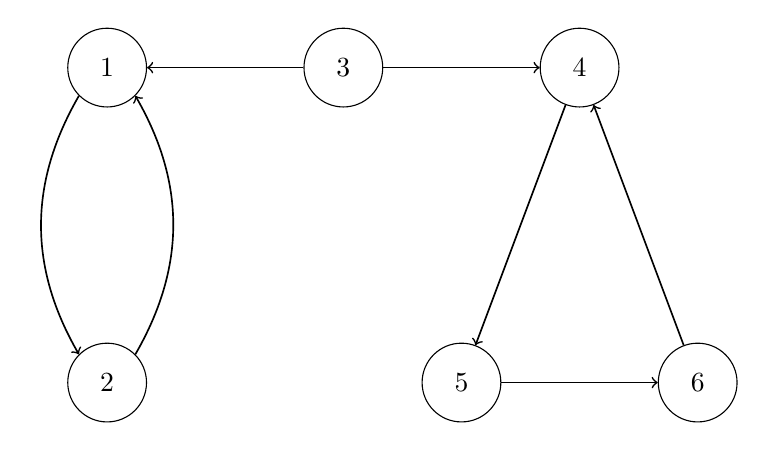
\begin{tikzpicture}
\node[shape=circle,draw, minimum size = 1cm] (N1) at (0, 4) {1};
\node[shape=circle,draw, minimum size = 1cm] (N2) at (0, 0) {2};
\node[shape=circle,draw, minimum size = 1cm] (N3) at (3, 4) {3};
\node[shape=circle,draw, minimum size = 1cm] (N4) at (6, 4) {4};
\node[shape=circle,draw, minimum size = 1cm] (N5) at (4.5, 0) {5};
\node[shape=circle,draw, minimum size = 1cm] (N6) at (7.5, 0) {6};
\draw[->, semithick] (N1.south west) to[out=240, in=120] (N2.north west);
\draw[->, semithick] (N2.north east) to[out=60, in=-60] (N1.south east);
\draw[->, semithick] (N3) -- (N1);
\draw[->, semithick] (N3) -- (N4);
\draw[->, semithick] (N4) -- (N5);
\draw[->, semithick] (N5) -- (N6);
\draw[->, semithick] (N6) -- (N4);
\end{tikzpicture}
\caption[Beispiel einer Markovkette mit verschiedenen Typen von Zust�nden]{Beispiel einer Markovkette mit verschiedenen Typen von Zust�nden.}\label{fig:markov2}
\end{figure}

\begin{definition}[Erreichbarkeit, Kommunizierend]\label{Nummer3.4.1}
Sei $(X_n)_{n \geq 0}$ eine homogene Markovkette mit �bergangsmatrix $\P$ und Startverteilung $\alpha$. F�r $i, j \in S$ sagen wir,
\begin{enumerate}
	\item dass $j$ von $i$ aus \deftxt{erreichbar}\index{Zustand!erreichbarer} ist und schreiben $i \to j$ genau dann, wenn ein $m \geq 0$ mit $p_{i,j}^{(m)} > 0$ existiert.
	\item dass $i$ und $j$ \deftxt{kommunizieren}\index{Zustand!kommunizierender} und schreiben $i \leftrightarrow j$ genau dann, wenn $i \to j$ und $j \to i$ gilt.
\end{enumerate}
\end{definition}

Wir erinnern uns daran, dass wir $p_{ij}^{(0)} = \delta_{ij}$ definiert haben und daher $i \leftrightarrow j$ f�r alle $i \in S$ gilt. Ferner ist $i \to j$ genau dann, wenn es einen Pfad von $i$ nach $j$ gibt. Dies ist im Wesentlichen die Aussage von Chapman-Kolmogorov (vergleiche Satz \ref{Nummer3.1.4}). Die �quivalenzrelation "`$\leftrightarrow$"' beschreibt die sog. \emph{starken Zusammenhangskomponenten} des Graphen, wenn man die Kanten $(i,i)$ hinzuf�gt. Die zugeh�rigen �quivalenzklassen hei�en \deftxt{Kommunikationsklassen}\index{Kommunikationsklasse}. Im Beispiel aus Abbildung \ref{fig:markov2} w�ren dies $\{1,2\}$, $\{3\}$ und $\{4,5,6\}$.

Ist $C$ eine Kommunikationsklasse und sind $i, j \in C$, so existiert ein Pfad in $C$, der von $i$ nach $j$ f�hrt. F�r den Beweis nehmen wir an, dass es $i, j \in C$ gibt, so dass jeder Pfad von $i$ nach $j$ durch ein $l \in S \setminus C$ verl�uft. Solch einen Pfad mit $l \notin C$ wollen wir nun fixieren, dann gilt $i \to l$ und $l \to j \to i$. Damit gilt aber $i \leftrightarrow l$ und daher $l \in C$, was einen Widerspruch darstellt.

Unser n�chstes Ziel ist die Beschreibung von Zustandsmengen, aus denen wir nicht wieder herauskommen k�nnen. Dazu f�hren wir den folgenden Begriff ein:

\begin{definition}[Abgeschlossene Menge]\label{Nummer3.4.2}
Es sei $(X_n)_{n \geq 0}$ eine homogene Markovkette mit �bergangsmatrix $\P$ und Startverteilung $\alpha$. Eine Menge $A \subset S$ hei�t \deftxt{abgeschlossen}\index{Abgeschlossene Menge} genau dann, wenn gilt
\begin{align*}
\sum_{j \in A} p_{ij} &= 1 \qquad \text{f�r alle } i \in A\text{.}
\end{align*}
\end{definition}

Mit anderen Worten existiert also kein $j \notin A$ mit $p_{ij} > 0$. Im Beispiel aus Abbildung \ref{fig:markov2} w�ren $\{1,2\}$, $\{4,5,6\}$ oder auch $\{1,2,4,5,6\}$ und $S$ selbst abgeschlossene Mengen.

\begin{definition}[Irreduzibilit�t]\label{Nummer3.4.3}
Es sei $(X_n)_{n \geq 0}$ eine homogene Markovkette. Eine Menge $A \subset S$ hei�t \deftxt{irreduzibel}\index{Irreduzibilit�t} genau dann, wenn $i \leftrightarrow j$ f�r alle $i, j \in A$ gilt. Ferner nennen wir die Markovkette $(X_n)$ selbst \deftxt{irreduzibel}\index{Markovkette!irreduzible} genau dann, wenn $S$ irreduzibel ist.
\end{definition}

Aus der Irreduzibilit�t folgt im Allgemeinen nicht die Abgeschlossenheit. Dazu kann man Zustand 3 in Abbildung \ref{fig:markov2} betrachten. Ist $S$ irreduzibel, so ist eine Kommunikationsklasse namensgebend. Die gr��te irreduzible Menge, die ein $i \in S$ enth�lt, ist dessen Kommunikationsklasse. Im Allgemeinen sind Kommunikationsklassen aber nicht abgeschlossen.

Wir sind nun an der Wahrscheinlichkeit daf�r interessiert, dass man in endlicher Zeit von $i$ nach $j$ gelangen kann. Die Wahrscheinlichkeit, nach genau $m$ Schritten von $i$ nach $j$ zu gelangen, haben wir mit $p_{ij}^{(m)}$ bezeichnet. 

F�r $j \in S$ definieren wir die \deftxt{R�ckkehrzeit}\index{R�ckkehrzeit}
\begin{align*}
\tau_j &:= \inf\{n \geq 1 : X_n = j\}\text{.}
\end{align*}
F�r diese Stoppzeit gilt $\tau_j \geq 1$, insbesondere gilt also $X_0(\omega) = j \not\Rightarrow \tau_j(\omega) = 0$. F�r $i, j \in S$ setzen wir nun
\begin{align*}
\rho_{i,j} &:= P(\tau_j < \infty \mid X_0 = i)\text{.}
\end{align*}
Daher beschreibt $\rho_{i,j}$ gerade die Wahrscheinlichkeit daf�r, in endlicher Zeit zu $j$ zu gelangen, wenn man in $i$ startet. Insbesondere ist $\rho_{i,i}$ gerade die R�ckkehrwahrscheinlichkeit. Gelangen wir sicher in endlicher Zeit von $i$ nach $i$, ist also $\rho_{i,i} = 1$, so liegt aufgrund der starken Markoveigenschaft die Vermutung nahe, dass $i$ unendlich oft besucht wird. Wir werden sehen, dass $i$ nur endlich oft besucht wird, wenn $\rho_{i,i} < 1$ ist.

\begin{definition}[Transienz, Rekurrenz]\label{Nummer3.4.4}
Es sei $(X_n)_{n \geq 0}$ eine homogene Markovkette. Ein Zustand $i \in S$ hei�t dann
\begin{enumerate}
	\item \deftxt{transient}\index{Transienz} genau dann, wenn $\rho_{i,i} < 1$ ist.
	\item \deftxt{rekurrent}\index{Rekurrenz} genau dann, wenn $\rho_{i,i} = 1$ ist.
	\item \deftxt{positiv rekurrent}\index{Rekurrenz!positive} genau dann, wenn der Zustand rekurrent ist und zus�tzlich $\E(\tau_i \mid X_0 = i) < \infty$ gilt.
	\item \deftxt{nullrekurrent}\index{Rekurrenz!Null-} genau dann, wenn der Zustand rekurrent ist und $\E(\tau_i \mid X_0 = i) = \infty$ gilt.
\end{enumerate}
\end{definition}

Jeder Zustand $i \in S$ ist offenbar entweder transient oder rekurrent. Au�erdem ist jeder rekurrente Zustand entweder positiv rekurrent oder nullrekurrent. F�r $i \in S$ setzen wir nun
\begin{align*}
N_i &:= \sum_{n=0}^\infty \ind_{\{X_n = i\}}
\end{align*}
f�r die Anzahl der Besuche in $i$. Dann gilt $\E(N_i \mid X_0 = i) = \sum_{n=0}^\infty P(X_n=i \mid X_0=i) = \sum_{n=0}^\infty p_{ii}^{(n)}$ f�r die erwarteten Besuche in $i$. Ferner betrachten wir die Wahrscheinlichkeit daf�r, dass $X_n = i$ unendlich oft eintritt. Diese ist gegeben durch
\begin{align*}
P(N_i = \infty \mid X_0=i) &= P(\limsup \{X_n = i\} \mid X_0=i)\text{.}
\end{align*} 
Wir erwarten nun, dass diese Gr��en f�r transiente und (positive bzw. null-)rekurrente Zust�nde unterschiedlich sind.

\begin{satz}\label{Nummer3.4.5}
Sei $(X_n)_{n \geq 0}$ eine homogene Markovkette und $i \in S$.
\begin{enumerate}
	\item Ist $i$ rekurrent, so gilt $P(N_i = \infty \mid X_0 = i) = 1$ und $\E(N_i \mid X_0=i) = \sum_{n=0}^\infty p_{ii}^{(n)} = \infty$.
	\item Ist $i$ transient, so gilt $P(N_i = \infty \mid X_0 = i) = 0$ und $\E(N_i \mid X_0=i) = \sum_{n=0}^\infty p_{ii}^{(n)} = \frac{1}{1-\rho_{i,i}} < \infty$.
\end{enumerate}
\end{satz}

\begin{beweis}
Wir betrachten die letzte Besuchszeit, die gegeben ist durch
\begin{align*}
L_i\colon \Omega &\to \overline{\N_0}\text{,}\\
L_i(\omega) &:= \sup\{n \geq 0 : X_n(\omega) = i\}\text{.}
\end{align*}
Es gilt zu beachten, dass $L_i$ keine Stoppzeit definiert, da die Zukunft $X_m(\omega) \neq i$ f�r $m > n$ beschrieben wird. Ist $X_0(\omega) = i$, so folgt $\{n \geq 0 : X_n(\omega) = i\} \neq \emptyset$ und $L_i(\omega) \geq 0$. Als Vorbemerkung f�hren wir folgende Rechnung an: 
\begin{align*}
P(A \cap C \mid B) &= \frac{P(A \cap C \cap B)}{P(B)} = \frac{P(A \cap C \cap B)}{P(B \cap C)} \cdot \frac{P(B \cap C)}{P(B)} = P(A \mid B \cap C) \cdot P(C \mid B)\text{.}
\end{align*}
Damit erhalten wir f�r $n \geq 0$
\begin{align*}
P(L_i = n \mid X_0 = i) &\stackrel{\hphantom{\text{\ref{Nummer3.3.3}}}}{=} P(X_n = i \text{ und } X_m \neq i\,\forall_{m > n} \mid X_0 = i)\\
\quad &\stackrel{\hphantom{\text{\ref{Nummer3.3.3}}}}{=} P(X_m \neq i\,\forall_{m > n} \mid X_n = i \text{ und } X_0 = i) \cdot P(X_n = i \mid X_0 = i)\\
\quad &\stackrel{\text{\ref{Nummer3.3.3}}}{=} P(X_m \neq i\,\forall_{m > 0} \mid X_0 = i) \cdot P(X_n = i \mid X_0 = i)\\
\quad &\stackrel{\hphantom{\text{\ref{Nummer3.3.3}}}}{=} (1-\rho_{i,i})p_{ii}^{(n)}\text{.} \tag{*}
\end{align*}
Summieren wir �ber diesen Ausdruck, so erhalten wir
\begin{align*}
P(L_i < \infty \mid X_0 = i) &= (1-\rho_{i,i}) \sum_{n=0}^\infty p_{ii}^{(n)}\\
\quad &= (1 - \rho_{i,i}) \E(N_i \mid X_0 = i)\text{.}
\end{align*}
Ferner besucht $(X_n)$ den Zustand $i$ genau dann unendlich oft, wenn $L_i = \infty$ ist. Damit folgt
\begin{align*}
P(L_i < \infty \mid X_0 = i) &= 1 - P(N_i = \infty \mid X_0 = i)\text{.} \tag{**}
\end{align*}
Setzen wir dies zusammen, so erhalten wir
\begin{align*}
(1-\rho_{i,i}) \E(N_i \mid X_0 = i) &= 1 - P(N_i = \infty \mid X_0 = i)\text{.} \tag{***}
\end{align*}
Ist $i$ rekursiv, so gilt per Definition $\rho_{i,i} = 1$. Wegen (*) folgt damit $P(L_i = n \mid X_0 = i) = 0$ f�r alle $n \geq 0$ und damit $P(L_i < \infty \mid X_0 = i) = 0$. Aus (**) folgt dann, dass $P(N_i = \infty \mid X_0 = i) = 1$ gilt. Mit dem Lemma von Borel-Cantelli\footnote{Dieses findet sich im Anhang unter Lemma \ref{appendix:borelcantelli2}.} folgt dann
\begin{align*}
\E(N_i \mid X_0 = i) &= \sum_{n=1}^\infty P(X_n = i \mid X_0 = i) = \infty\text{.}
\end{align*}
Ist $i$ hingegen transient, so gilt $\rho_{i,i} < 1$ und mit (***) folgt daher
\begin{align*}
\E(N_i \mid X_0 = i) &= \frac{1 - P(N_i = \infty \mid X_0 = i)}{1 - \rho_{i,i}} < \infty\text{.}
\end{align*}
Mit dem Lemma von Borel-Cantelli folgt dann wiederum $P(N_i = \infty \mid X_0 = i) = 0$ und mit (***) schlie�lich
\begin{align*}
\E(N_i \mid X_0 = i) &= \frac{1}{1 - \rho_{i,i}}\text{.} \qedhere
\end{align*}
\end{beweis}

\begin{satz}[Abh�ngigkeit von Kommunikationsklassen]\label{Nummer3.4.6}
Es sei $(X_n)_{n \geq 0}$ eine homogene Markovkette und $i, j \in S$ mit $i \leftrightarrow j$. Dann gilt:
\begin{enumerate}
	\item $i$ ist rekurrent genau dann, wenn $j$ rekurrent ist.
	\item $i$ ist transient genau dann, wenn $j$ transient ist.
\end{enumerate}
\end{satz}

\begin{beweis}
Da jeder Zustand entweder transient oder rekurrent ist, m�ssen wir lediglich die erste Aussage beweisen. Da diese zudem symmetrisch in $i$ und $j$ ist, gen�gt es, nur eine Implikation zu beweisen. Sei daher $i$ transient. Dann folgt wegen der kommunizierenden Eigenschaft, dass es $k, m \geq 0$ mit $p_{ij}^{(k)} > 0$ und $p_{ji}^{(m)} > 0$ gibt. Dann gilt mit dem Satz von Chapman-Kolmogorov aber $p_{ii}^{(k+l+m)} \geq p_{ij}^{(k)}p_{jj}^{(l)}p_{ji}^{(m)}$ f�r alle $l \geq 0$. Summieren wir �ber $l$, so erhalten wir
\begin{align*}
\sum_{l=0}^\infty p_{jj}^{(l)} &\leq \frac{1}{p_{ij}^{(k)}p_{ji}^{(m)}}\sum_{l=0}^\infty p_{ii}^{(k+l+m)} < \infty\text{,}
\end{align*}
da $i$ nach Voraussetzung transient war. Damit ist $j$ nicht rekurrent und daher transient.
\end{beweis}

Satz \ref{Nummer3.4.6} garantiert die Wohldefiniertheit der folgenden Sprechweise: Wir sagen, dass eine Kommunikationsklasse $A$ \deftxt{rekurrent}\index{Rekurrenz} bzw. \deftxt{transient}\index{Transienz} hei�t, wenn es einen rekurrenten bzw. transienten Zustand $i \in A$ gibt, da dies dann auch f�r alle anderen Zust�nde in $A$ gilt.

\begin{satz}[Abgeschlossenheit von Kommunikationsklassen]\label{Nummer3.4.7}
Es sei $(X_n)_{n \geq 0}$ eine homogene Markovkette und $R \subset S$ eine rekurrente Kommunikationsklasse. Dann ist $R$ abgeschlossen im Sinne von Definition \ref{Nummer3.4.2}.
\end{satz}

\begin{beweis}
Wir nehmen an, dass $R$ nicht abgeschlossen ist. Dann existieren $i \in R$, $j \notin R$ und $m \geq 0$ mit $P(X_m = j \mid X_0 = i) > 0$. Da $R$ eine Kommunikationsklasse ist, in der $j$ nicht enthalten ist, gilt au�erdem $P(X_n = i \text{ und } X_m = j \mid X_0 = i) = 0$ f�r alle $n > m$. Dann folgt auch $P(X_n = i \text{ unendlich oft und } X_m = j \mid X_0 = i) = 0$. Wir erhalten
\begin{align*}
P(X_n = i \text{ $\infty$-oft} \mid X_0 = i) &\leq P(X_n = i \text{ $\infty$-oft und } X_m = j \mid X_0 = i) + P(X_m \neq j \mid X_0 = i)\\
\quad &\leq 0 + (1 - P(X_m = j))\\
\quad &< 1\text{.}
\end{align*}
Mit Satz \ref{Nummer3.4.5} folgt dann, dass $i$ nicht rekurrent ist. Nach Satz \ref{Nummer3.4.6} stellt dies jedoch einen Widerspruch dar.
\end{beweis}

\begin{satz}[Zerlegung des Zustandsraumes]\label{Nummer3.4.8}
Es sei $(X_n)_{n \geq 0}$ eine homogene Markovkette. Dann l�sst sich der Zustandsraum zerlegen in
\begin{align*}
S &= T \cup \bigcup_{l \in L} R_l\text{,}
\end{align*}
wobei $T$ die Menge der transienten Zust�nde, $L$ eine h�chstens abz�hlbare Indexmenge und $R_l$ f�r jedes $l \in L$ eine irreduzibele, abgeschlossene und rekurrente Kommunikationsklasse ist.
\end{satz}

\begin{figure}[!htbp]
\centering
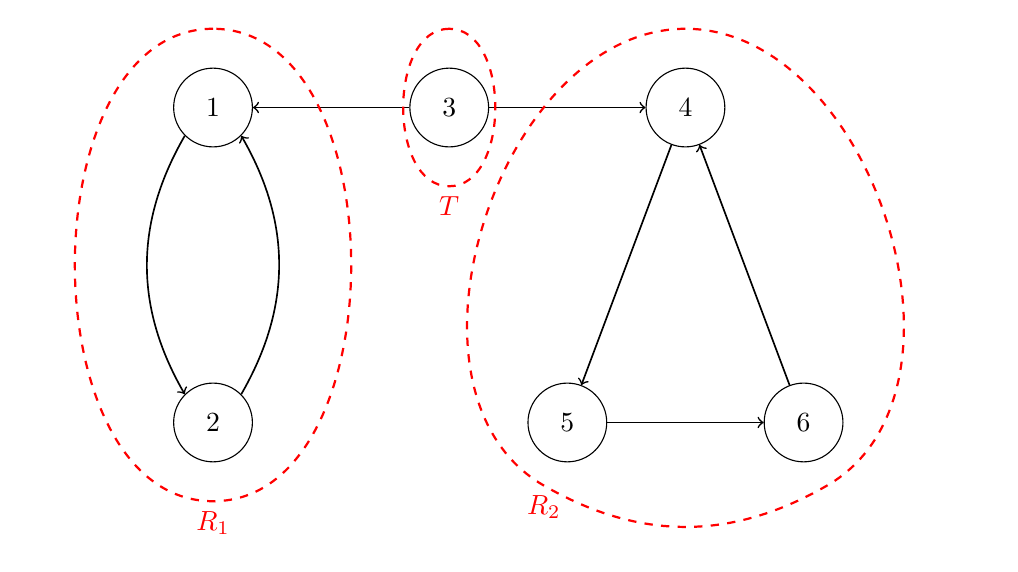
\begin{tikzpicture}
\node[shape=circle,draw, minimum size = 1cm] (N1) at (0, 4) {1};
\node[shape=circle,draw, minimum size = 1cm] (N2) at (0, 0) {2};
\node[shape=circle,draw, minimum size = 1cm] (N3) at (3, 4) {3};
\node[shape=circle,draw, minimum size = 1cm] (N4) at (6, 4) {4};
\node[shape=circle,draw, minimum size = 1cm] (N5) at (4.5, 0) {5};
\node[shape=circle,draw, minimum size = 1cm] (N6) at (7.5, 0) {6};
\draw[->, semithick] (N1.south west) to[out=240, in=120] (N2.north west);
\draw[->, semithick] (N2.north east) to[out=60, in=-60] (N1.south east);
\draw[->, semithick] (N3) -- (N1);
\draw[->, semithick] (N3) -- (N4);
\draw[->, semithick] (N4) -- (N5);
\draw[->, semithick] (N5) -- (N6);
\draw[->, semithick] (N6) -- (N4);

\draw[red, thick, dashed] (0, 5) to[out=180, in=180] (0,-1) node[below] {$R_1$} to[out=0, in=0] (0,5);
\draw[red, thick, dashed] (3, 5) to[out=180, in=180] (3,3) node[below] {$T$} to[out=0, in=0] (3,5);
\draw[red, thick, dashed] (6, 5) to[out=180, in=150] (4.2,-0.8) node[below] {$R_2$} to[out=-30, in=210] (7.8,-0.8) to[out=30, in=0] (6,5);
\end{tikzpicture}
\caption[Zerlegung einer Markovkette in transiente und rekurrente Teile]{Zerlegung des Beispiels aus Abbildung \ref{fig:markov2} gem�� Satz \ref{Nummer3.4.8}.}\label{fig:markov3}
\end{figure}

\begin{beweis}
Seien $(C_k)_{k \in K}$ die Kommunikationsklassen, dann ist $S = \bigcup_{k \in K} C_k$ eine paarweise disjunkte Vereinigung, wobei $K$ h�chstens abz�hlbar ist, da auch $S$ h�chstens abz�hlbar ist. Wir setzen nun $T$ als die Vereinigung �ber die transienten $C_k$. Dann gilt
\begin{align*}
S &= T \quad \cup \bigcup_{\substack{k \in K\\C_k\text{ rekurrent}}} \hspace{-1.5em}C_k\text{.}
\end{align*}
Mit Satz \ref{Nummer3.4.7} ist jede rekurrente Kommunikationsklasse aber auch abgeschlossen. Da Kommunikationsklassen zudem nach Definition irreduzibel sind, folgt die Behauptung.
\end{beweis}

Eine Menge $A \subset S$ ist abgeschlossen, wenn kein Pfad $A$ verl�sst und irreduzibel, wenn es f�r jedes $i \in A$ einen Pfad zu jedem $j \in A$ gibt. Ist $A$ endlich, abgeschlossen und irreduzibel, so w�rden wir erwarten, dass jeder Zustand h�ufig besucht wird.

\begin{satz}[Rekurrenz endlicher, irreduzibler Markovketten]\label{Nummer3.4.9}
Sei $(X_n)_{n \geq 0}$ eine homogene Markovkette und $A \subset S$ endlich, abgeschlossen und irreduzibel. Dann ist $A$ positiv rekurrent.
\end{satz}

Insbesondere sind also auch endliche, irreduzible und abgeschlossene Markovketten bereits positiv rekurrent.

\begin{beweis}
Es sei $i \in A$, dann gilt $i \leftrightarrow j$ f�r alle $j \in A$ und daher existiert f�r alle $j \in A$ ein $k_j$ mit $P(\tau_i \leq k_j \mid X_0 = j) > 0$. Da $A$ endlich ist, k�nnen wir das Maximum $k := \max\{k_j : j \in A\} < \infty$ w�hlen. Nun sei
\begin{align*}
\e &:= P(\tau_i \leq k \mid X_0 = j) > 0\text{.} \tag{*}
\end{align*}
Wir wollen zeigen, dass $P(\tau_i > nk \mid X_0 = j) = (1-\e)^n$ ist und f�hren hierf�r eine vollst�ndige Induktion durch. Der Induktionsanfang ist bereits in (*) gegeben. F�r den Induktionsschritt beachten wir nun, dass $\tau_i \leq k$ genau dann gilt, wenn $X_{\tau_i \wedge k} = i$ ist. Dann gilt
\begin{align*}
P(\tau_i > (n+1)k \mid X_0 = j) &= P(X_{\tau_i \wedge (n+1)k} \neq i \mid X_0 = j)\\
\quad &= \sum_{i \neq l \in A} P(X_{\tau_i \wedge (n+1)k} \neq i, X_{\tau_i \wedge nk} = l \mid X_0 = j)\\
\quad &= \sum_{i \neq l \in A} P(X_{\tau_i \wedge (n+1)k} \neq i \mid X_{\tau_i \wedge nk} = l, X_0 = j)P(X_{\tau_i \wedge nk} = l \mid X_0 = j)\text{.}
\intertext{Wir wenden auf den ersten Faktor die starke Markoveigenschaft und (*) an und erhalten}
\quad &= (1-\e) \sum_{i \neq l \in A} P(X_{\tau_i \wedge nk} = l \mid X_0 = j)\\
\quad &= (1-\e) (1-\e)^n\\
\quad &= (1-\e)^{n+1}\text{.}
\end{align*}
Mit einem Satz aus der Wahrscheinlichkeitstheorie und dem Integral-Vergleichskriterium folgt dann
\begin{align*}
\E(\tau_i \mid X_0 = i) &= \int_0^\infty P(\tau_i \geq t \mid X_0 = i)~\dd t = \sum_{n=0}^\infty P(\tau_i > n \mid X_0 = i)\\
\quad &\leq k\sum_{n=0}^\infty P(\tau_i > nk \mid X_0 = i)\\
\quad &< \infty\text{.} \qedhere
\end{align*}
\end{beweis}

\begin{korollar}\label{Nummer3.4.10}
Sei $(X_n)_{n \geq 0}$ eine homogene Markovkette und $A \subset S$ eine endliche Kommunikationsklasse. Dann sind die folgenden Aussagen �quivalent:
\begin{enumerate}
	\item\label{N3410A1} $A$ ist abgeschlossen.
	\item\label{N3410A2} $A$ ist rekurrent.
	\item\label{N3410A3} $A$ ist positiv rekurrent.
\end{enumerate}
\end{korollar}

\begin{beweis}
F�r \ref{N3410A1} $\Rightarrow$ \ref{N3410A3} folgt, nach Satz \ref{Nummer3.4.9}, dass $A$ irreduzibel ist, da $A$ nach Voraussetzung eine Kommunikationsklasse ist. Der Schritt \ref{N3410A3} $\Rightarrow$ \ref{N3410A2} ist offensichtlich und \ref{N3410A2} $\Rightarrow$ \ref{N3410A1} folgt schlie�lich aus Satz \ref{Nummer3.4.7}.
\end{beweis}

Wir k�nnen zusammenfassend also sagen, dass wir endliche Kommunikationsklassen bez�glich der Rekurrenz gut verstehen. Die n�chste Frage w�re also, wie es mit unendlichen Kommunikationsklassen aussieht. Hier lassen sich solche Aussagen nicht treffen, wie wir im folgenden Beispiel sehen werden.

\begin{beispiel}[Irrfahrt auf $\Z$]\label{Nummer3.4.11}
Sei $(Y_n)_{n \geq 0}$ i.\,i.\,d. mit $P(Y_n = 1) =: p \in (0,1)$ und $P(Y_n = -1) = 1-p$. Dann setzen wir $X_n := \sum_{i=0}^n Y_n$ und in Beispiel \ref{Nummer3.2.5} haben wir bereits gesehen, dass dies eine homogene Markovkette mit $p_{i,i+1} = p$ und $p_{i, i-1} = 1-p$ f�r $i \in \Z$ und $p_{i,j} = 0$ sonst ist. Dass $(X_n)$ irreduzibel ist, ist klar, da $i \leftrightarrow i+1$ f�r alle Zust�nde $i \in \Z$ gilt. Au�erdem gilt $X_n = 0$ $P$-fast sicher und es gen�gt, die Rekurrenz in $i = 0$ zu untersuchen. Man kann sich leicht �berlegen, dass $p_{0,0}^{(2n+1)} = 0$ f�r alle $n \geq 0$ gilt. 

Wie sieht es f�r eine gerade Anzahl von Schritten aus? Gelangen wir von $0$ nach $0$ in $2n$ Schritten, so m�ssen wir genau $n$ Schritte in eine und $n$ Schritte in die andere Richtung machen. Die Wahrscheinlichkeit von einer solchen Folge von Schritten betr�gt $p^n(1-p)^n$ und es gibt $\binom{2n}{n}$ verschiedene solcher Folgen. Damit erhalten wir
\begin{align*}
p_{0,0}^{(2n)} &= \binom{2n}{n} p^n (1-p)^n\text{.}
\end{align*}
Mit Satz \ref{Nummer3.4.5} reicht es, die Reihe $\sum_{n=0}^\infty p_{0,0}^{(2n)}$ zu untersuchen. Dazu verwenden wir die Stirling-Formel\footnote{Siehe \cite[Satz 1.8.6]{WT}.}, die im Wesentlichen $n! \sim \sqrt{2\pi n} \left(\frac{n}{e}\right)^n$ besagt. Damit erhalten wir
\begin{align*}
\binom{2n}{n} = \frac{(2n)!}{(n!)^2} &\sim \frac{4^n}{\sqrt{\pi n}}\text{.}
\end{align*}
Im ersten Fall sei $p = 1-p$, dann ist $4^n p^n (1-p)^n = 1$ und wir erhalten
\begin{align*}
\sum_{n = 0}^\infty p_{0,0}^{(2n)} &\geq c \sum_{n=0}^\infty \frac{1}{\sqrt{\pi n}} = \infty\text{,}
\end{align*}
also ist die Irrfahrt rekurrent. Im zweiten Fall sei $p \neq 1-p$, dann gilt $4^n (1-p)^n = a^n$ f�r ein $a \in (0,1)$. Dann ist die Reihe konvergent und die Irrfahrt daher transient.
\end{beispiel}

Man kann zeigen, dass die symmetrische Irrfahrt in $\Z^d$ genau dann rekurrent ist, wenn $d \leq 2$ ist. Anschaulich gesprochen bewegt man sich stets um die $0$ herum. F�r Details verweisen wir auf \cite[S. 248]{MEINTRUP}.

Satz \ref{Nummer3.4.6} hatte f�r einen rekurrenten Zustand $i$ mit $i \leftrightarrow j$ gezeigt, dass dann auch $j$ rekurrent ist. Dies wollen wir nun verallgemeinern.

\begin{satz}[Allgemeine Erreichbarkeitswahrscheinlichkeiten]\label{Nummer3.4.12}
Sei $(X_n)_{n \geq 0}$ eine homogene Markovkette und $i \in S$ ein rekurrenter Zustand. F�r $j \in S$ betrachten wir
\begin{align*}
\rho_{i,j} &:= P(\tau_j < \infty \mid X_0 = i)\text{.}
\end{align*}
Gilt $i \rightarrow j$, so ist auch $j$ rekurrent und es gilt $\rho_{i,j} = \rho_{j,i} = 1$.
\end{satz}

\begin{beweis}
Es sei also $i \rightarrow j$. Dann existieren paarweise verschiedene $i_0, \ldots, i_k$ mit $i_0 = i$, $i_k = j$ und $P(X_1 = i_1, \ldots, X_k = i_k \mid X_0 = i) > 0$, insbesondere gilt also $p_{i,j}^{(k)} > 0$. Nun folgt
\begin{align*}
0 = 1 - \rho_{i,i} &= P(\tau_i = \infty \mid X_0 = i)\\
\quad &\geq P(X_1 = i_1, \ldots, X_k = i_k, \tau_i = \infty \mid X_0 = i)\\
\quad &= P(X_1 = i_1, \ldots, X_k = i_k \mid X_0 = i)P(\tau_i = \infty \mid X_l = i_l \text{ f�r } l = 0, \ldots, k)
\intertext{und mit der Markoveigenschaft erhalten wir}
\quad &= P(X_1 = i_1, \ldots, X_k = i_k \mid X_0 = i)P(\tau_i = \infty \mid X_0 = i_k)\\
\quad &= \underbrace{P(X_1 = i_1, \ldots, X_k = i_k \mid X_0 = i)}_{> 0} (1 - \rho_{j,i})\text{.}
\end{align*}
Damit folgt $1-\rho_{j,i} = 0$ und daher $\rho_{j,i} = 1$. Daher existiert ein $l \geq 1$ mit $p_{j,i}^{(l)} > 0$ und f�r $n \geq 0$ folgt mit der Chapman-Kolmogorov-Gleichung $p_{j,j}^{(l + n + k)} \geq p_{j,i}^{(l)}p_{i,i}^{(n)}p_{i,j}^{(k)}$. Dann gilt
\begin{align*}
\E(N_j \mid X_0 = j) &\stackrel{\text{\ref{Nummer3.4.5}}}{=} \sum_{n=0}^\infty p_{j,j}^{(n)} \geq \sum_{n=0}^\infty p_{j,i}^{(l)}p_{i,i}^{(n)}p_{i,j}^{(k)} = p_{j,i}^{(l)}p_{i,j}^{(k)} \sum_{n=0}^\infty p_{i,i}^{(n)} = \infty\text{,} 
\end{align*}
da $i$ rekurrent ist. Wieder mit Satz \ref{Nummer3.4.5} folgt also, dass auch $j$ rekurrent ist. Vertauschen wir die Rollen von $i$ und $j$, so folgt der Rest. 
\end{beweis}
	\section{Stationarit�t}

Wir wollen untersuchen, ob es zu einer gegebenen �bergangsmatrix $\P$ eine Startverteilung $\alpha$ gibt, so dass die homogene Markovkette station�r ist. Dazu beobachten wir, dass zu einem gegebenen $\P$ jede Startverteilung eine homogene Markovkette ergibt, deren Irreduzibilit�t und Rekurrenz von $\alpha$ unabh�ngig ist. Im Folgenden schreiben wir $P_\alpha$ statt $P$, wenn die Wahrscheinlichkeiten der Markovkette mit der Startverteilung $\alpha$ betrachtet werden.

\begin{definition}[Stationarit�t]\label{Nummer3.5.1}
Sei $\P$ eine stochastische Matrix �ber $S$. Eine Verteilung $\pi$ auf $S$ hei�t \deftxt{station�r}\index{Stationarit�t} bez�glich $\P$ genau dann, wenn f�r alle $j \in S$ gilt:
\begin{align*}
\sum_{i \in S} \pi(i)p_{i,j} &= \pi(j)\text{.}
\end{align*}
\end{definition}

Anschaulich ausgedr�ckt ist die Wahrscheinlichkeit, im ersten Schritt nach $j$ zu gelangen, wenn der Start $i$-verteilt ist, also $\pi(j)$. In der Matrixschreibweise gilt also $\pi\P = \pi$ und $\pi$ ist ein Eigenvektor von $\P$ zum Eigenwert $1$.

\begin{satz}[Station�re homogene Markovketten]\label{Nummer3.5.2}
Sei $\P$ eine stochastische Matrix und $\pi$ eine station�re Verteilung von $\P$, sowie $\alpha$ irgendeine Startverteilung und $(X_n)_{n \geq 0}$ die homogene Markovkette bez�glich $\alpha$ und $\P$. F�r $B \in \bigotimes_{\N} \Pot(S)$ gilt dann
\begin{align*}
P_\pi((X_n, X_{n+1}, \ldots) \in B) &= P_\pi((X_0, X_1, \ldots) \in B)\text{.}
\end{align*}
\end{satz}

Satz \ref{Nummer3.5.2} besagt also, dass $(\pi, P)$ eine station�re, homogene Markovkette definiert.

\begin{beweis}
Wir wissen, dass $\pi\P = \pi$ gilt. Induktiv folgt dann auch $\pi\P^n = \pi$ f�r $n \geq 1$. Mit Lemma \ref{Nummer3.2.3} folgt dann
\begin{align*}
P_\pi(X_n = j) &= \sum_{i \in S} \pi(j)p_{i,j}^{(n)} = \pi(j)\text{.}
\end{align*}
Damit erhalten wir
\begin{align*}
P_\pi((X_n, X_{n+1}, \ldots) \in B) &= \sum_{i \in S} P_\pi(X_n = i)P_\pi((X_n, \ldots) \in B \mid X_n = i)\\
\quad &= \sum_{i \in S} \pi(i)P_\pi((X_0, \ldots) \in B \mid X_0 = i)\\
\quad &= P_\pi((X_0, \ldots) \in B)\text{.} \qedhere
\end{align*}
\end{beweis}

Wir wollen nun Bedingungen f�r die Existenz station�rer Verteilungen studieren.

\begin{lemma}[Positivit�t station�rer Verteilungen]\label{Nummer3.5.3}
Sei $\pi$ eine station�re Verteilung bez�glich $\P$ und $A \subset S$ abgeschlossen und irreduzibel. Gibt es ein $i_0 \in A$ mit $\pi(i_0) > 0$, so gilt $\pi(i) > 0$ f�r alle $i \in A$. 
\end{lemma}

Ist $(X_n)_{n \geq 0}$ eine irreduzible, homogene Markovkette und $\pi$ eine station�re Verteilung dieser Markovkette, so folgt also insbesondere $\pi(i) > 0$ f�r alle $i \in S$.

\begin{beweis}
Wir setzen $S_+ := \{i \in A : \pi(i) > 0\}$ und $S_0 := \{i \in A : \pi(i) = 0\}$. Offenbar sind $S_+$ und $S_0$ disjunkt und es gilt $S_+ \neq \emptyset$ nach Voraussetzung. Zu zeigen ist nun $S_0 = \emptyset$. Wir nehmen an, dass $S_0 \neq \emptyset$ gilt, dann existiert also ein $j_0 \in S_0$ mit $\pi(j_0) = 0$. F�r $j \in S_0$ folgt
\begin{align*}
\sum_{i \in S} \pi(i)p_{i,j} &= \pi(j) = 0\text{.}
\end{align*}
Da $\pi(i) > 0$ f�r alle $i \in S_+$ gilt, folgt $p_{i,j}=0$ f�r alle $i \in S_+$ und $j \in S_0$. Es gibt also keine Verbindung von $S_+$ nach $S_0$, also gibt es keinen Pfad in $A$, der von $i_0$ nach $j_0$ f�hrt. Dies steht jedoch im Widerspruch zur Irreduzibilit�t von $A$.
\end{beweis}

\begin{satz}\label{Nummer3.5.4}
Sei $(X_n)_{n \geq 0}$ eine homogene Markovkette mit station�rer Verteilung $\pi$, $A \subset S$ abgeschlossen und irreduzibel und es existiere ein $i_0 \in A$ mit $\pi(i_0) > 0$. Dann gilt
\begin{align*}
\E(\tau_i \mid X_0 = i) &= \frac{P_\pi(\tau_i < \infty)}{\pi(i)}
\end{align*}
f�r alle $i \in A$. Insbesondere sind alle $i \in A$ positiv rekurrent und ist $(X_n)_{n \geq 0}$ irreduzibel, so gilt f�r alle $i \in S$
\begin{align*}
\pi(i) &= \frac{1}{\E(\tau_i \mid X_0 = i)}\text{,}
\end{align*}
das hei�t in diesem Fall ist $\pi$ eindeutig.
\end{satz}

\begin{beweis}
F�r $i \in S$ zeigen wir zun�chst
\begin{align*}
\pi(i)\E(\tau_i \mid X_0 = i) = P_\pi(\tau_i < \infty)\text{.} \tag{*}
\end{align*}
Dazu betrachten wir die disjunkte Zerlegung
\begin{align*}
\{\tau_i \leq n\} &= \bigcup_{l=1}^n \{X_l = i, X_{l+1} \neq i, \ldots, X_n \neq i\} = \bigcup_{l=0}^{n-1} \{X_{n-l} = i, X_{n-l+1} \neq i, \ldots, X_n \neq i\}\text{,}
\end{align*} 
dann folgt mit Satz \ref{Nummer3.5.2}
\begin{align*}
P_\pi(\tau_i < \infty) &= \lim_{n \to \infty} P_\pi(\tau_i \leq n) = \lim_{n \to \infty} \sum_{l=0}^{n-1} P_\pi(X_{n-l} = i, X_{n-l+1} \neq i, \ldots, X_n \neq i)\\
\quad &= \lim_{n \to \infty} \sum_{l=0}^{n-1} P_\pi(X_0 = i, X_1 \neq i, \ldots, X_l \neq i)\\
\quad &= \sum_{l=0}^\infty P(X_0 = i, \tau_i > l)\text{,}
\intertext{da $X_j \neq i$ genau dann gilt, wenn $\tau_i > l$ ist. Weiter folgt dann}
\quad &= \sum_{l=0}^\infty P_\pi(\tau_i > l \mid X_0 = i)P_\pi(X_0 = i)\\
\quad &= \sum_{l=0}^\infty P(\tau_i > l \mid X_0 = i)\pi(i)\\
\quad &= \pi(i) \E(\tau_i \mid X_0 = i)\text{.}
\end{align*}
Dies beweist (*). Sei nun $i \in A$, dann folgt mit Lemma \ref{Nummer3.5.3} wegen $\pi(i_0) > 0$ auch $\pi(i) > 0$. Wir k�nnen (*) daher durch $\pi(i)$ teilen und erhalten die gew�nschte Gleichung.

Ferner gilt mit Satz \ref{Nummer3.4.12} auch
\begin{align*}
P_\pi(\tau_i < \infty) &= \sum_{j \in S} P(\tau_i < \infty \mid X_0 = j)P_\pi(X_0 = j) = \sum_{j \in S} 1 \cdot \pi(j)\\
\quad &= 1\text{.} \qedhere
\end{align*}
\end{beweis}

\begin{satz}\label{Nummer3.5.5}
Ist $(X_n)_{n \geq 0}$ eine homogene Markovkette und $i \in S$ ein positiv rekurrenter Zustand, so existiert eine station�re Verteilung.
\end{satz}

\begin{beweis}
F�r $j \in S$ sei
\begin{align*}
c(j) &:= \sum_{n=0}^\infty P(X_n = j, \tau_i > n \mid X_0 = i)\text{.}
\end{align*}
Dann wollen wir zeigen, dass $\pi(j) := \frac{c_j}{\E(\tau_i \mid X_0 = i)}$ eine station�re Verteilung definiert. Wir zeigen zun�chst, dass $\pi$ eine Verteilung ist. Daf�r betrachten wir
\begin{align*}
\sum_{j \in S} c(j) &= \sum_{n=0}^\infty P(\tau_i > n \mid X_0 = i) = \E(\tau_i \mid X_0 = i) < \infty\text{.}
\end{align*}

F�r die Stationarit�t sei $c_n(j) := P(X_n = j, \tau_i > n \mid X_0 = i)$ f�r $n \geq 0$ und $j \in S$. Dann wollen wir zeigen, dass f�r alle $k \in S$
\begin{align*}
\sum_{j \in S} c(j)p_{jk} &= \sum_{n=0}^\infty \sum_{j \in S} c_n(j)p_{jk} \stackrel{\text{!}}{=} c(k)
\end{align*}
gilt. Im ersten Fall sei $i \neq k$. Da $\{\tau_i > n\} \in \sigma(X_0, \ldots, X_n)$ gilt, folgt
\begin{align*}
\sum_{n=0}^\infty \sum_{j \in S} c_n(j)p_{jk} &= \sum_{n=0}^\infty \sum_{j \in S} P(X_n=j, \tau_i > n \mid X_0 = i)P(X_{n+1} = k \mid X_n = j)\\
\quad &= \sum_{n=0}^\infty \sum_{j \in S} P(X_n = j, \tau_i > n \mid X_0 = i)P(X_{n+1} = k \mid X_n = j, \tau_i > n)\text{.}
\intertext{Mit der uns bereits bekannten Formel $P(A \cap C \mid B) = P(A \mid C \cap B)P(C \mid B)$ gilt dann}
\quad &= \sum_{n=0}^\infty \sum_{j \in S} P(X_n = j, X_{n+1} = k, \tau_i > n \mid X_0 = i)\\
\quad &= \sum_{n=0}^\infty P(X_{n+1} = k, \tau_i > n \mid X_0 = i)\text{.}
\intertext{Wegen $X_{n+1} = k \neq i$ folgt $\tau_i \neq n+1$ und daher}
\quad &= \sum_{n=0}^\infty P(X_{n+1} = k, \tau_i > n+1 \mid X_0 = i)\\
\quad &= \sum_{n=0}^\infty c_{n+1}(k)\text{.}
\intertext{Wegen $c_0(k) = P(X_0=k, \tau_i > n \mid X_0=i) = 0$ f�llt der erste Summand weg und wir erhalten}
\quad &= \sum_{n=0}^\infty c_n(k)\\
\quad &= c(k)\text{.}
\end{align*}
Im zweiten Fall sei $i=k$, dann erhalten wir zun�chst wie eben
\begin{align*}
\sum_{n=0}^\infty \sum_{j \in S} c_n(j)p_{ij} &= \sum_{n=0}^\infty P(X_{n+1} = i, \tau_i > n \mid X_0 = i)
\intertext{und nun mit $\tau_i > 0$ und $\tau_i < \infty$ $P$-fast sicher}
\quad &= \sum_{n=0}^\infty P(\tau_i = n+1 \mid X_0 = i)\\
\quad &= 1\\
\quad &= P(X_0 = i, \tau_i > 0 \mid X_0 = i)\\
\quad &= \sum_{n=0}^\infty P(X_n = i, \tau_i > n \mid X_0 = i)\text{.}
\intertext{Das Ereignis in der Summe ist f�r $n > 0$ aber nie erf�llt und wir erhalten schlie�lich}
\quad &= c(i)\text{.} \qedhere
\end{align*}
\end{beweis}

\begin{korollar}\label{Nummer3.5.6}
Es sei $(X_n)_{n \geq 0}$ eine irreduzible, homogene Markovkette. Dann sind die folgenden Aussagen �quivalent:
\begin{enumerate}
	\item\label{N356A1} Es existiert ein positiv rekurrenter Zustand $i \in S$.
	\item\label{N356A2} Alle Zust�nde $i \in S$ sind positiv rekurrent.
	\item\label{N356A3} Es existiert eine station�re Verteilung.
	\item\label{N356A4} Es existiert genau eine station�re Verteilung.
\end{enumerate}
Ist eine dieser Aussagen -- und damit alle -- erf�llt, so gilt f�r $i \in S$
\begin{align*}
\pi(i) &= \frac{1}{\E(\tau_i \mid X_0 = i)}\text{.}
\end{align*}
\end{korollar}

\begin{beweis}
F�r \ref{N356A1} $\Rightarrow$ \ref{N356A3} verwenden wir Satz \ref{Nummer3.5.5}, f�r \ref{N356A3} $\Rightarrow$ \ref{N356A4} und \ref{N356A3} $\Rightarrow$ \ref{N356A2} verwenden wir Satz \ref{Nummer3.5.4} und \ref{N356A2} $\Rightarrow$ \ref{N356A1} und \ref{N356A4} $\Rightarrow$ \ref{N356A3} sind trivial.
\end{beweis}
	\section{Grenzverhalten}

Wenn wir wissen, dass $i \in S$ transient ist, so folgt mit Satz \ref{Nummer3.4.5}, dass $p_{ii}^{(n)} \to 0$ gilt. Was gilt jedoch im Allgemeinen? Dazu betrachten wir
\begin{align*}
\P &:= \begin{pmatrix}0 & 1\\ 1 & 0\end{pmatrix}\text{,}
\end{align*}
dann gilt $\P^2 = E_2$, wobei $E_n$ die Einheitsmatrix ist. Wir erhalten also
\begin{align*}
\P^n &= \begin{cases}\P & \text{falls $n$ ungerade}\\ E_2 & \text{sonst}\end{cases}\text{.}
\end{align*}
Dann konvergiert $p_{ii}^{(n)}$ jedoch nicht. Ein solches periodisches Verhalten wollen wir also ausschlie�en.

\begin{definition}[Periodizit�t]\label{Nummer3.6.1}
Sei $(X_n)_{n \geq 0}$ eine homogene Markovkette und $i \in S$.
\begin{enumerate}
	\item Die \deftxt{Periode}\index{Periode} von $i$ ist der gr��te gemeinsame Teiler von 
	\begin{align*}
	J_i &:= \left\{n \geq 1 : p_{ii}^{(n)} > 0\right\}\text{.}
	\end{align*}
	\item Der Zustand $i$ hei�t \deftxt{aperiodisch}\index{Zustand!aperiodischer}, falls er die Periode $1$ hat.
\end{enumerate}
\end{definition}

Betrachten wir nochmal das obige Beispiel. Da $J_1 = J_2 = 2\N$ gilt, haben $i = 1$ und $i = 2$ jeweils die Periode $2$.

Beachte, dass $p_{ii}^{(n)} > 0$ genau dann gilt, wenn man in \emph{genau} $n$ Schritten von $i$ nach $i$ gelangen kann. In Abbildung \ref{fig:markovperiode} sehen wir einen g�ngigen Denkfehler f�r die Periode eines Zustandes.
\begin{figure}[!htbp]
\centering
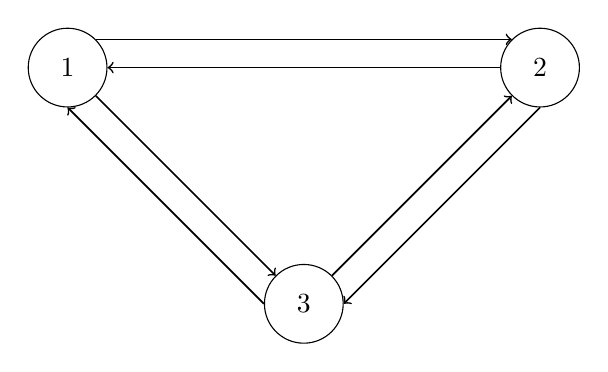
\begin{tikzpicture}
\node[shape=circle,draw, minimum size = 1cm] (N1) at (0, 3) {1};
\node[shape=circle,draw, minimum size = 1cm] (N3) at (3, 0) {3};
\node[shape=circle,draw, minimum size = 1cm] (N2) at (6, 3) {2};
\draw[->, semithick] (N1.north east) -- (N2.north west);
\draw[->, semithick] (N1.south east) -- (N3.north west);
\draw[->, semithick] (N2.west) 			 -- (N1.east);
\draw[->, semithick] (N2.south) 		 -- (N3.east);
\draw[->, semithick] (N3.west) 			 -- (N1.south);
\draw[->, semithick] (N3.north east) -- (N2.south west);
\end{tikzpicture}
\caption[Periodizit�t in Markovketten]{Von jedem Zustand $i$ gelangt man in sowohl zwei als auch drei Schritten von $i$ nach $i$, die Periode ist daher $1$.}\label{fig:markovperiode}
\end{figure}

\begin{lemma}\label{Nummer3.6.2}
Sei $A \subset \N$ mit $\ggT(A) = 1$ und $A$ sei abgeschlossen bez�glich der Addition. Dann existiert ein $n_0$, so dass $n \in A$ f�r alle $n \geq n_0$ gilt.
\end{lemma}

\begin{beweis}
Da die Aussage rein zahlentheoretischer Natur ist, wollen wir sie hier nicht beweisen und verweisen stattdessen auf \cite[Lemma 9.41]{MEINTRUP}.
\end{beweis}

\Needspace{6\baselineskip}\begin{lemma}\label{Nummer3.6.3}
Sei $(X_n)_{n \geq 0}$ eine homogene Markovkette und $i \in S$. Dann sind folgende Aussagen �quivalent:
\begin{enumerate}
	\item\label{N363A1} Der Zustand $i$ ist aperiodisch.
	\item\label{N363A2} Es existiert ein $n_0$, so dass $p_{ii}^{(n)} > 0$ f�r alle $n \geq n_0$ gilt.
\end{enumerate}
\end{lemma}

\begin{beweis}
F�r \ref{N363A1} $\Rightarrow$ \ref{N363A2} setzen wir $A := \{n \geq 0 : p_{ii}^{(n)} > 0\}$. Da $i$ aperiodisch ist, gilt $\ggT(A) = 1$. F�r $n, m \in A$ gilt ferner $p_{ii}^{(n+m)} \geq p_{ii}^{(n)}p_{ii}^{(m)} > 0$ und daher $n+m \in A$. Mit Lemma \ref{Nummer3.6.2} folgt dann die Aussage.

F�r \ref{N363A2} $\Rightarrow$ \ref{N363A1} sei $d = \ggT(A)$. Nach Voraussetzung existiert ein $n_0$ mit der entsprechenden Eigenschaft. Also gilt $d \mid n_0$ und $d \mid n_0 + 1$. Dann teilt $d$ aber auch $(n_0+1) - n_0 = 1$ und wir erhalten $d=1$.
\end{beweis}

\begin{satz}\label{Nummer3.6.4}
Ist $(X_n)_{n \geq 0}$ eine homogene Markovkette, $i \in S$ aperiodisch und $A \subset S$ die Kommunikationsklasse von $i$, so existiert ein $n_0$, so dass $p_{jk}^{(n)} > 0$ f�r alle $j, k \in A$ und alle $n \geq n_0$ gilt.

Setzen wir $j = k$, so folgt insbesondere, dass $j$ aperiodisch ist.
\end{satz}

\begin{beweis}
Es seien $j, k \in A$. Dann existieren $l, m \geq 0$ mit $p_{ji}^{(l)} > 0$ und $p_{ij}^{(k)} > 0$. Mit Lemma \ref{Nummer3.6.3} existiert dann ein $n_0$, so dass $p_{ii}^{(n)} > 0$ f�r alle $n \geq n_0$ gilt. Damit erhalten wir
\begin{align*}
p_{jk}^{(l + n + m)} &\geq p_{ji}^{(l)}p_{ii}^{(n)}p_{ik}^{(m)} > 0\text{.} \qedhere
\end{align*}
\end{beweis}

\begin{definition}[Kopplung]\label{Nummer3.6.5}
Es seien $(X_n)_{n \geq 0}$ und $(Y_n)_{n \geq 0}$ stochastische Prozesse �ber $(\Omega, \sA, P)$ mit Zustandsraum $\sX$. Dann sind $(X_n)$ und $(Y_n)$ ein \deftxt{Kopplungspaar}\index{Kopplung}, falls eine $P$-fast sicher endliche Stoppzeit $\tau$ existiert, so dass f�r alle $n \geq 0$ und $\omega \in \Omega$ gilt:
\begin{align*}
n \geq \tau(\omega) &\Longrightarrow X_n(\omega) = Y_n(\omega)\text{.}
\end{align*}
Wir nennen $\tau$ in diesem Fall \deftxt{Kopplungszeit}\index{Kopplungszeit}.
\end{definition}

Aneinander gekoppelte stochastische Prozesse sind nach der Zeit $\tau$ also gleich.

\begin{satz}[Konvergenz von Kopplungen]\label{Nummer3.6.6}
Es sei $\tau$ die Kopplungszeit zum Kopplungspaar $(X_n)$ und $(Y_n)$. F�r eine messbare Menge $A \subset \sX$ gilt dann
\begin{align*}
\lim_{n \to \infty} \left(P(X_n \in A) - P(Y_n \in A)\right) &= 0\text{.}
\end{align*}
\end{satz}

Beachte: Der Grenzwert $\lim P(X_n \in A)$ selbst existiert im Allgemeinen nicht.

\begin{beweis}
Wir betrachten
\begin{align*}
\vert P(X_n \in A) - P(Y_n \in A) \vert &\leq \vert P(X_n \in A, \tau \leq n) - P(Y_n \in A, \tau \leq n) \vert\\
\quad &\hspace{3em}+ \vert P(X_n \in A, \tau > n) - P(Y_n \in A, \tau > n) \vert\\
\quad &\leq 2P(\tau > n)\\
\quad &\to 0\text{.} \qedhere
\end{align*}
\end{beweis}

\minisec{Konstruktion von Produkt-Markovketten}

Es seien $(X_n)_{n \geq 0}$ und $(Y_n)_{n \geq 0}$ unabh�ngige, homogene Markovketten bez�glich $(\alpha, \P)$ und $(\beta, \P)$, sie unterscheiden sich also nur in ihrer Startverteilung. Es sei $Z_n := (X_n, Y_n) \in S \times S$, dann kann man leicht zeigen, dass $(Z_n)_{n \geq 0}$ eine homogene Markovkete auf $S \times S$ mit Startverteilung $\alpha \otimes \beta$ und der �bergangsmatrix $\overline{\P}$ verm�ge
\begin{align*}
\overline{p}_{(i_0, j_0), (i_1, j_1)} &= p_{i_0, i_1} p_{j_0, j_1}
\end{align*}
bildet.

\begin{satz}\label{Nummer3.6.7}
Es seien $(X_n)_{n \geq 0}$, $(Y_n)_{n \geq 0}$ und $(Z_n)_{n \geq 0}$ wie eben definiert. Ist $(Z_n)_{n \geq 0}$ irreduzibel und rekurrent, so gelten die folgenden Aussagen:
\begin{enumerate}
	\item\label{N367A1} Die Stoppzeit $\tau_{i_0} := \inf\{n \geq 1 : X_n = Y_n = i_0\}$ f�r $i_0 \in S$ ist $P$-fast sicher endlich.
	\item\label{N367A2} Es sei
	\begin{align*}
	W_n &:= \begin{cases} X_n & \text{falls } n \leq \tau_{i_0}\\ Y_n & \text{falls } n > \tau_{i_0}\end{cases}\text{.}
	\end{align*}
	Dann ist $W_n$ eine homogene Markovkette mit Startverteilung $\alpha$ bez�glich $\P$.
	\item\label{N367A3} F�r alle $A \subset S$ gilt
	\begin{align*}
	P(X_n \in A) - P(Y_n \in A) &\to 0\text{.}
	\end{align*}
\end{enumerate}
\end{satz}

\begin{beweis}
F�r den Beweis von \ref{N367A1} betrachten wir die R�ckkehrzeit $\tau = \tau_{i_0}$ von $(Z_n)$ zum Zustand $(i_0, i_0)$. Da $(Z_n)$ rekurrent ist, gilt $P$-fast sicher $\tau < \infty$.

Die Aussage \ref{N367A2} werden wir hier nicht beweisen. Wir verweisen stattdessen auf \cite[S. 258]{MEINTRUP}.

F�r \ref{N367A3} beachten wir, dass $(Y_n)$ und $(W_n)$ f�r $\tau_{i_0}$ ein Kopplungspaar sind. Nach \ref{N367A2} sind $(W_n)$ und $(X_n)$ identisch verteilt, da beide Markovketten bez�glich $(\alpha, \P)$ sind. Dann wenden wir Satz \ref{Nummer3.6.6} an.
\end{beweis}

\begin{satz}[Konvergenz homogener Markovketten]\label{Nummer3.6.8}
Es sei $(X_n)_{n \geq 0}$ eine irreduzible, homogene Markovkette mit station�rer Verteilung $\pi$. Dann gilt
\begin{align*}
P(X_n = j) &\stackrel{n \to \infty}{\longrightarrow} \pi(j)
\end{align*}
f�r alle $j \in S$.

Ist $\alpha = \delta_{\{i\}}$, so gilt insbesondere $p_{ij}^{(n)} \to \pi(j)$ f�r alle $i, j \in S$.
\end{satz}

\begin{beweis}
Es sei $(\alpha, \P)$ die Konfiguration von $(X_n)_{n \geq 0}$ und $(Y_n)_{n \geq 0}$ eine von $(X_n)_{n \geq 0}$ unabh�ngige, homogene Markovkette mit der Konfiguration $(\pi, \P)$. Wir wollen zeigen, dass $Z_n := (X_n, Y_n)$ irreduzibel und rekurrent ist, um Satz \ref{Nummer3.6.7} anzuwenden. F�r die Irreduzibilit�t seien $(i_0, j_0), (i_1, j_1) \in S \times S$, dann folgt mit Lemma \ref{Nummer3.6.3}, dass ein $r \geq 0$ mit $p_{i_1,i_1}^{(r)} > 0$ und $p_{j_1, j_1}^{(r)} > 0$ existiert. Mit Lemma \ref{Nummer3.6.3} folgt dann $p_{i_0,i_1}^{(n)}p_{j_0,j_1}^{(n)} > 0$ f�r alle $n \geq 0$. Damit erhalten wir
\begin{align*}
\overline{p}_{(i_0, j_0),(i_1, j_1)}^{(n+r)} &= p_{i_0, i_1}^{(r)}p_{j_0, j_1}^{(r)} > 0\text{,}
\end{align*}
also ist $Z_n$ irreduzibel. F�r die Rekurrenz kann man leicht zeigen, dass $\pi \otimes \pi$ eine station�re Verteilung von $(X_n, Y_n)$ ist. Nach Korollar \ref{Nummer3.5.6} ist $(Z_n)$ also rekurrent. Mit Satz \ref{Nummer3.6.7} erhalten wir
\begin{align*}
P(X_n = j) - \pi(j) &= P(X_n = j) - P(Y_n = j) \longrightarrow 0\text{.} \qedhere
\end{align*}
\end{beweis}

F�r endliche Zustandsr�ume $S$ l�sst sich der Beweis auch elementarer f�hren. Hierf�r verweisen wir auf die Literatur.

Es sei $(X_n)_{n \geq 0}$ irreduzibel und aperiodisch. Dann wollen wir folgende Eigenschaften festhalten:
\begin{enumerate}
	\item Ist $(X_n)$ zus�tzlich transient, so gilt
	\begin{align*}
	\sum_n p_{ij}^{(n)} &\leq \frac{1}{p_{ji}^{(r)}} \sum_n p_{ij}^{(n)}p_{ji}^{(r)} \leq \frac{1}{p_{ji}^{(r)}} \sum_n p_{ii}^{(n+r)} < \infty\text{.}
	\end{align*}
	Also gilt $p_{ij}^{(n)} \to 0$.
	\item Ist $(X_n)_{n \geq 0}$ positiv rekurrent, so existiert nach Korollar \ref{Nummer3.5.6} eine station�re Verteilung $\pi$ mit $\pi(j) > 0$ f�r alle $j \in S$. Nach Satz \ref{Nummer3.6.8} gilt dann $p_{ij}^{(n)} \to \pi(j)$ und $\sum_n p_{ij}^{(n)} = \infty$.
	\item Den dritten Fall halten wir in Satz \ref{Nummer3.6.9} fest.
\end{enumerate}

\begin{satz}\label{Nummer3.6.9}
Sei $(X_n)_{n \geq 0}$ eine irreduzible, aperiodische und rekurrente, aber nicht positiv rekurrente, homogene Markovkette. F�r alle $i, j \in S$ gilt dann
\begin{align*}
p_{ij}^{(n)} &\longrightarrow 0
\end{align*}
und
\begin{align*}
\sum_n p_{ij}^{(n)} &= \infty\text{.}
\end{align*}
\end{satz}

\begin{beweis}
Der Beweis findet sich in \cite[Satz 9.48]{MEINTRUP} und wird hier nicht gef�hrt.
\end{beweis}
\chapter{Poissonprozesse}

\begin{beschreibung}
Poissonprozesse sind spezielle Z�hlprozesse mit poissonverteilten Zuw�chsen, die zum Beispiel das wiederholte Eintreten eines Ereignisses modellieren.
\end{beschreibung}

\section{Definition und Eigenschaften}

Im Folgenden betrachten wir einen $\N_0$-wertigen stochastischen Prozess $(X_t)_{t \geq 0}$ mit kontinuierlicher Zeit. Satz \ref{Nummer1.2.7} besagte, dass $X$ genau dann rechtsstetig ist, wenn f�r alle $\omega \in \Omega$ und alle $t > 0$ ein $\e > 0$ mit $X_s(\omega) = X_t(\omega)$ f�r alle $s \in [t, t+\e)$ existiert. Der Prozess ist rechts von Stetigkeitsstellen also in einer gewissen Umgebung konstant. Insbesondere gibt es f�r jede Trajektorie genau drei M�glichkeiten:
\begin{enumerate}
	\item Die Trajektorie besitzt endlich viele Spr�nge.
	\item Die Trajektorie hat unendlich viele Spr�nge, aber nur endlich viele in jedem beschr�nkten Intervall.
	\item Es gibt ein Zeitintervall, in welchem unendlich viele Spr�nge auftreten. Man spricht in diesem Fall von \emph{Explosionen}.
\end{enumerate}
Wir werden sehen, dass bei Poissonprozessen $P$-fast sicher nur der zweite Fall eintritt. Daher wollen wir diese Eigenschaft n�her untersuchen. In der Abbildung \ref{poisson1} sehen wir einen solchen Prozess und die Bezeichnungen f�r die entsprechenden Zeiten, die wir in diesem Kapitel verwenden wollen. Wir sehen bereits, dass eine solche Nummerierung der $T_i$ im dritten Fall nicht ohne Weiteres m�glich w�re und dass wir im ersten Fall nur endlich viele $T_i$ haben.

\begin{figure}[!htbp]
\centering
\begin{tikzpicture}
\draw[semithick, ->] (-0.5,0) -- (10,0);
\draw[semithick, ->] (0,-0.5) -- (0,6);
\draw[red, thick, o-)] (0, 1) -- node[above] {$S_0$} (2, 1);
\draw[red, thick, o-)] (2, 3.5) -- node[above] {$S_1$} (6, 3.5);
\draw[red, thick, o-)] (6, 5) -- node[above] {$S_2$} (7.5, 5);
\draw[red, thick, o-)] (7.5, 2) -- node[above] {$S_3$} (8.5, 2);
\draw[red, thick, o-)] (8.5, 1) -- node[above] {$S_4$} (10, 1);
\draw (2, -0.15) -- (2, 0.15);
\draw (6, -0.15) -- (6, 0.15);
\draw (7.5, -0.15) -- (7.5, 0.15);
\draw (8.5, -0.15) -- (8.5, 0.15);
\draw (0, -0.5) node[below] {\small $T_0$};
\draw (2, -0.5) node[below] {\small $T_1$};
\draw (6, -0.5) node[below] {\small $T_2$};
\draw (7.5, -0.5) node[below] {\small $T_3$};
\draw (8.5, -0.5) node[below] {\small $T_4$};
\draw (1, 0) node[below] {\small $W_1$};
\draw (4, 0) node[below] {\small $W_2$};
\draw (6.75, 0) node[below] {\small $W_3$};
\draw (8, 0) node[below] {\small $W_4$};
\draw (9.25, 0) node[below] {\small $W_5$};
\end{tikzpicture}
\caption[Darstellung eines rechtsstetigen, zeitkontinuierlichen Prozesses]{Die Abbildung zeigt eine typische Trajektorie eines rechtsstetigen, zeitkontinuierlichen stochastischen Prozesses, sowie die Bezeichnungen f�r dieses Kapitel.}\label{poisson1}
\end{figure}

Im zweiten Fall l�sst sich $(X_t)_{t \geq 0}$ vollst�ndig durch die Angabe der Werte $(S_n)_{n \geq 1}$ und der Sprungzeiten $(T_n)_{n \geq 0}$ bzw. durch Angabe der Werte $(S_n)_{n \geq 0}$ und der Wartezeiten $(W_n)_{n \geq 1}$ beschreiben. Die Rechtsstetigkeit und der diskrete Zustandsraum erlaubt es uns also, einen zeitkontinuierlichen Prozess durch zwei zeitdiskrete Prozesse zu beschreiben. Dies wollen wir nun formalisieren.

\begin{definition}[Sprungprozesse]\label{Nummer4.1.1}
Sei $(X_t)_{t \geq 0}$ ein zeitkontinuierliches, rechtsstetiger und $\N_0$-wertiger stochastischer Prozess. 
\begin{enumerate}
	\item Die \deftxt{Sprungzeiten}\index{Sprungzeit} $(T_n)_{n \geq 0}$ sind definiert durch $T_0 := 0$ und $\displaystyle T_{n+1} := \inf\{t \geq T_n : X_t \neq X_{T_n}\}$ f�r $n > 0$ mit $\inf \emptyset := \infty$.
	\item Der Prozess $(X_t)$ hei�t \deftxt{explosionsfrei}\index{Stochastischer Prozess!explosionsfreier}, wenn $P$-fast sicher $\displaystyle\lim_{n \to \infty} T_n = \infty$ gilt.
	\item Die \deftxt{Wartezeiten}\index{Wartezeit} $(W_n)_{n \geq 1}$ sind definiert durch
	\begin{align*}
	W_n &:= \begin{cases}T_n - T_{n-1} & \text{falls } T_{n-1} < \infty\\\infty & \text{sonst}\end{cases}\text{.}
	\end{align*}
	\item Der \deftxt{Sprungprozess}\index{Sprungprozess} $(S_n)_{n \geq 0}$ ist definiert durch
	\begin{align*}
	S_n &:= \begin{cases} X_{T_n} & \text{falls } T_n < \infty\\ X_{T_m} & \text{sonst}\end{cases}\text{,}
	\end{align*}
	wobei $m := \max\{r \in \N_0 : T_r < \infty\}$ die letzte endliche Sprungzeit beschreibt.
\end{enumerate}
\end{definition}

Besitzt ein Pfad nur endlich viele Spr�nge, so sind sowohl Warte- als auch Sprungzeit nach dem letzten Sprung unendlich. Ist $T_{n-1} < \infty$, so besagt Satz \ref{Nummer1.2.7}, dass $T_{n-1} < T_n$ gilt. Der Satz besagt au�erdem $W_n > 0$. 

Ist $(X_t)$ explosionsfrei, so bestimmen $(S_n)$ und $(W_n)$ bzw. $(S_n)$ und $(T_n)$ den Prozess $(X_t)_{t \geq 0}$ durch $X_n = S_n$ f�r $T_n \leq t < T_{n+1}$.

\begin{satz}\label{Nummer4.1.2}
Sei $(W_n)_{n \geq 1}$ i.\,i.\,d. mit $W_i \in \sL_1$ und $P(W_n \in (0, \infty)) = 1$. F�r $n \geq 0$ und $t \geq 0$ setzen wir $T_n := \sum_{i=1}^n W_i$ und $X_t := \sum_{i=1}^\infty \ind_{(0, t]}(T_i)$ als die Anzahl der Spr�nge bis zur Zeit $t$. Dann ist $(X_t)_{t \geq 0}$ ein $\N_0$-wertiger, rechtsstetiger, monoton wachsender und explosionsfreier stochastischer Prozess, dessen Wartezeiten die $(W_n)_{n \geq 1}$ sind und dessen Sprungprozess $(S_n)$ durch $S_n = n$ f�r $n \geq 0$ gegeben ist. F�r alle $n \geq 0$ gilt ferner $P$-fast sicher $T_n < \infty$ und $T_n < T_{n+1}$.
\end{satz}

\begin{beweis}
Es gilt $P(T_{n+1} - T_n > 0) = P(W_{n+1} > 0) = 1$. F�r $n \geq 0$ und $t \geq 0$ folgt damit $\{X_t = n\} = \{T_n \leq t < T_{n+1}\}$. Wir wollen zeigen, dass $P$-fast sicher $X_t \in \N_0$ f�r alle $t \geq 0$ gilt. Dazu betrachten wir
\begin{align*}
\{X_t = \infty\} &= \{\lim T_n \leq t\} = \left\{\sum_{i=1}^\infty W_i \leq t\right\} = \left\{\sum_{i=1}^n W_i \leq t \quad \forall_{n \geq 0}\right\} = \left\{0 \leq \frac{1}{n}\sum_{i=1}^n W_i \leq \frac{t}{n} \quad \forall_{n \geq 0}\right\}\\
\quad &\subset \left\{\lim \frac{1}{n} \sum_{i=1}^n W_i = 0\right\}\text{.}
\end{align*}
Das starke Gesetz der gro�en Zahlen impliziert nun $P$-fast sicher $\frac{1}{n} \sum_{i=1}^n W_i \to \E W_1 > 0$ und wir erhalten $P(X_t = \infty) = 0$. 

Wir wollen nun zeigen, dass $(X_t)$ explosionsfrei ist. Da $(X_t)$ offenbar monoton wachsend und $\N_0$-wertig ist, ist keine Explosion m�glich, denn w�re bei $t_0$ eine Explosion, so h�tten wir $\lim_{t \nearrow t_0} X_t = \infty$ und damit g�be es $t < t_0$ mit $X_t > X_{t_0} \in \N_0$, was im Widerspruch zur Monotonie steht.

Wir zeigen nun, dass $(X_t)$ rechtsstetig ist. Dazu sei $t \geq 0$, $\omega \in \Omega$ und $n := X_t(\omega)$. Wegen $T_n < T_{n+1}$ existiert dann $\e > 0$ mit $T_n(\omega) \leq t+\e < T_{n+1}(\omega)$ $P$-fast sicher. Dann gilt $X_s(\omega) = n$ f�r alle $s \in [t, t+\e)$ und mit Satz \ref{Nummer1.2.7} folgt dann die Rechtsstetigkeit.

Ferner gilt wegen der Monotonie der $T_n$
\begin{align*}
X_{T_n} &= \sum_{i=0}^\infty \ind_{(0, T_n]}(T_i) = \sum_{i=1}^n \ind_{(0, T_n]}(T_i) = n \tag{*}\text{.}
\end{align*} 
Nun wollen wir zeigen, dass die $T_n$ die Sprungzeiten von $(X_t)$ sind. Dazu seien $(\tilde{T}_n)$ die Sprungzeiten von $(X_t)$ und wir zeigen mit vollst�ndiger Induktion, dass $T_n = \tilde{T}_n$ gilt. F�r den Induktionsanfang betrachte einfach $T_0 = 0 = \tilde{T}_0$. F�r den Induktionsschritt gilt
\begin{align*}
\tilde{T}_{n+1} &= \inf\{t \geq \tilde{T}_n : X_t \neq X_{\tilde{T}_n}\} = \inf\{t \geq T_n : X_t \neq X_{T_n}\} \stackrel{\text{(*)}}{=} \inf\left\{t \geq T_n : \sum_{i=0}^\infty \ind_{(0, t]}(T_i) \neq n\right\}\text{.}
\intertext{Wir k�nnen nun die Summe in $\sum_{i=0}^n \ind_{(0, t]}(T_i) + \sum_{i=n+1}^\infty \ind_{(0, t]}(T_i)$ aufspalten, wobei die erste dieser Teilsummen gerade $n$ ergibt. Wir erhalten daher aus der Nicht-Negativit�t}
\quad &= \inf\left\{t \geq T_n : \sum_{i=n+1}^\infty \ind_{(0, t]}(T_i) > 0\right\} = \inf\{t \geq T_n : t \geq T_{n+1}\}\\
\quad &= T_{n+1}\text{.}
\end{align*}

Wir zeigen nun noch, dass $P$-fast sicher $T_n < \infty$ gilt. Es ist $T_n = \sum_{i=1}^n W_i$ und wegen $P(W_i < \infty) = 1$ ist dann auch $P(T_n < \infty) = 1$. Damit sind die $W_n$ die Wartezeiten von $(X_t)$. Schlie�lich gilt mit (**) noch $S_n = X_{T_n} = n$.
\end{beweis}

Sind $(W_n)$, $(T_n)$ und $(X_t)$ wie im Satz \ref{Nummer4.1.2} gegeben, so hei�t $(X_t)_{t \geq 0}$ \deftxt{Z�hlprozess}\index{Z�hlprozess}, da dieser Prozess z�hlt, wie viele der konsekutiven Ereignisse, die zu den Zeiten $T_i$ eintreten, bereits zur Zeit $t$ eingetreten sind. Satz \ref{Nummer4.1.2} erm�glicht recht allgemein die Konstruktion solcher Z�hlprozesse.

Wir werden als n�chstes Poissonprozesse einf�hren, die Z�hlprozesse mit exponentialverteilten Wartezeiten sind. Daher wollen wir zun�chst die Exponentialverteilung\index{Exponentialverteilung} $\Exp(\lambda)$ f�r $\lambda > 0$ in Erinnerung rufen. Dies ist eine Lebesgue-absolut stetige Verteilung auf $\R$, welche durch die Dichte
\begin{align*}
h(t) &:= \begin{cases} \lambda\exp(-\lambda t) & \text{falls } t \geq 0\\ 0 & \text{sonst}\end{cases}
\end{align*}
gegeben ist. Ist $Y \sim \Exp(\lambda)$, so gelten die folgenden Eigenschaften:
\begin{enumerate}
	\item Es ist $P(Y \in (0, \infty)) = 1$.
	\item Es gilt $\E Y = \lambda^{-1}$ und $\Var Y = \lambda^{-2}$.
	\item Die Verteilungsfunktion von $Y$ ist gegeben durch
	\begin{align*}
	F_Y(t) &:= \begin{cases}1 - \exp(-\lambda t) & \text{falls } t \geq 0\\ 0 & \text{sonst}\end{cases}\text{.}
	\end{align*}
	\item Die Zufallsvariable $Y$ ist ged�chtnislos, f�r alle $t, s \geq 0$ gilt also
	\begin{align*}
	P(Y > t + s \mid Y > s) &= P(Y > t)\text{.}
	\end{align*}
	\item Sind $Y_1, \ldots, Y_n \sim \Exp(\lambda)$ unabh�ngig, so gilt $\sum_{i=1}^n Y_i \sim \Gamma(n, \lambda)$, wobei dies die Gammaverteilung\index{Gammaverteilung} ist, welche durch die Lebesgue-Dichte 
	\begin{align*}
	h_n(t) &:= \begin{cases}\lambda\frac{(\lambda t)^{n-1}}{(n-1)!}\exp(-\lambda t) & \text{falls } t > 0\\ 0 & \text{sonst}\end{cases}
	\end{align*}
	gegeben ist.
\end{enumerate}

Mit diesen elementaren Eigenschaften k�nnen wir nun zur Definition des Poissonprozesses, der ein Spezialfall von Satz \ref{Nummer4.1.2} darstellt. Dieser sichert die Existenz, die Explosionsfreiheit und das Vorhandensein unendlich vieler Spr�nge, insbesondere also auch $P$-fast sicher $T_n < \infty$ und $W_n < \infty$.

\begin{definition}[Poissonprozess]\label{Nummer4.1.3}
Ein rechtsstetiger und $\N_0$-wertiger stochastischer Prozess $(N_t)_{t \geq 0}$ hei�t \deftxt{homogener Poissonprozess}\index{Poissonprozess}\index{Poissonprozess!homogener} mit \deftxt{Rate}\index{Rate} $\lambda > 0$, wenn die folgenden Eigenschaften erf�llt sind:
\begin{enumerate}
	\item Es gilt $P$-fast sicher $N_0 = 0$.
	\item Die Wartezeiten $(W_n)_{n \geq 1}$ sind i.\,i.\,d. mit $W_n \sim \Exp(\lambda)$.
	\item Der Sprungprozess $(S_n)$ erf�llt $S_n = n$ f�r alle $n \geq 0$.
\end{enumerate}
\end{definition}

Poissonprozesse sind durch den Parameter $\lambda$ bereits eindeutig beschrieben, da Wartezeiten und Sprungprozess den stochastischen Prozess bereits festlegen.
	\section{�quivalente Beschreibung}

Wir wollen uns nun der Frage widmen, wieso Poissonprozesse ihren Namen tragen und daf�r eine �quivalente Beschreibung dieser Prozesse angeben.

\begin{satz}[Charakterisierung]\label{Nummer4.2.1}
Ein $\N_0$-wertiger, rechtsstetiger stochastischer Prozess $(N_t)_{t \geq 0}$ ist genau dann ein homogener Poissonprozess mit Rate $\lambda > 0$, wenn die folgenden Eigenschaften erf�llt sind:
\begin{enumerate}
	\item\label{N421A1} Es gilt $P$-fast sicher $N_0 = 0$.
	\item\label{N421A2} Der Prozess $(N_t)$ hat unabh�ngige Zuw�chse.
	\item\label{N421A3} Die Zuw�chse sind poissonverteilt, f�r $s, t \geq 0$ gilt also $N_{s+t} - N_s \sim \Pois(\lambda t)$.
\end{enumerate}
\end{satz}

Bevor wir diesen Satz beweisen, erinnern wir zun�chst daran, dass $\Pois(\lambda)$ durch die Dichte $\frac{\lambda^k}{k!}e^{-\lambda}$ bez�glich des Z�hlma�es auf $\N_0$ gegeben ist. Ferner weisen wir darauf hin, dass \ref{N421A3} impliziert, dass die Zuw�chse station�r sind und f�r $s=0$ folgt mit \ref{N421A1} auch $N_t \sim \Pois(\lambda t)$. Insbesondere gilt $\E N_t = \lambda t$, das hei�t im Intervall $[0, t]$ treten im Mittel $\lambda t$ Ereignisse ein. Pro Zeiteinheit treten im Mittel also $\lambda$ Ereignisse ein, es gilt also $\frac{\E N_t}{t} = \lambda$, wie wir eben schon gesehen haben. Diese Tatsache erkl�rt den Begriff \emph{Rate} f�r den Parameter $\lambda$.

Um Satz \ref{Nummer4.2.1} zu beweisen, ben�tigen wir zun�chst zwei Lemmata, die wir zun�chst behandeln.

\begin{lemma}\label{Nummer4.2.2}
Sei $\alpha_n\colon \R^n \to \R$ gegeben durch $x \mapsto \sum_{i=1}^n x_i$. F�r $t \geq 0$ gilt dann
\begin{align*}
\int_0^\infty \cdots \int_0^\infty \ind_{\{\alpha_n(x) \leq t\}}~\dd x_1 \cdots \dd x_n &= \frac{t^n}{n!}\text{.}
\end{align*}
\end{lemma}

Aufgrund der Nicht-Negativit�t des Integranden k�nnen wir das Integral mit dem Satz von Tonelli auch als Integral �ber das Produktma� schreiben oder die Integrationsreihenfolge beliebig ver�ndern.

\begin{beweis}
F�r den Beweis f�hren wir eine vollst�ndige Induktion durch. F�r $n = 1$ betrachten wir
\begin{align*}
\int_0^\infty \ind_{\{\alpha_1(x) \leq t\}}~\dd x &= \int_0^t 1~\dd x = t = \frac{t^1}{1!}\text{.}
\end{align*}
Wir kommen nun zum Induktionsschritt. Es gilt
\begin{align*}
\int_0^\infty \cdots \int_0^\infty \ind_{\{\alpha_{n+1}(x) \leq t\}}~\dd x_1 \cdots \dd x_n &= \int_0^\infty \cdots \int_0^\infty \ind_{\{\alpha_n(x) \leq t - x_{n+1}\}}\ind_{\{x_{n+1} \leq t\}}~\dd x_1 \cdots \dd x_n\\
\quad &= \int_0^t \frac{(t - x_{n+1})^n}{n!}~\dd x_{n+1}\\
\quad &= \frac{t^{n+1}}{(n+1)!}\text{.} \qedhere
\end{align*}
\end{beweis}

\begin{lemma}\label{Nummer4.2.3}
Sei $(N_t)_{t \geq 0}$ ein homogener Poissonprozess mit Rate $\lambda > 0$. Dann gilt f�r alle $s, t \geq 0$ f�r den Zuwachs $N_{s+t} - N_s \sim \Pois(\lambda t)$ und dieser Zuwachs ist von $\sigma(N_r : r \leq s)$ unabh�ngig.
\end{lemma}

\begin{beweis}
Wir wollen f�r $r \leq s$, $k, l \in \N_0$ zun�chst zeigen, dass
\begin{align*}
P(N_r = k, N_{s+t} - N_s = l) &= \exp(-\lambda r)\frac{(\lambda r)^k}{k!}\exp(-\lambda t)\frac{(\lambda t)^l}{l!} \tag{*}
\end{align*}
gilt. Wir betrachten zun�chst den Spezialfall $r = s$ und die Wartezeiten $(W_n)_{n \geq 1}$. Wir wissen, dass die Wartezeiten unabh�ngig und identisch verteilt sind mit $W_n \sim \Exp(\lambda)$. Die Dichte $h$ von $(W_n)_{n=1}^{k+l+1}$ ist daher das Temsorprodukt der einzelnen Dichten, das hei�t f�r $x \geq 0$ ist $h\colon \R^{k+l+1} \to \R$ gegeben durch
\begin{align*}
x &\mapsto \prod_{i=1}^{k+l+1} \lambda e^{-\lambda x_i} = \lambda^{k+l+1} \exp\left(-\lambda \alpha_{k+l+1}(x)\right)\text{,}
\end{align*}
wobei $\alpha_n$ wie in Lemma \ref{Nummer4.2.2} gegeben ist. Da $N_r = n$ �quivalent zu $T_n \leq r < T_{n+1}$ ist, erhalten wir
\begin{align*}
P(N_s = k, N_{s+t}-N_s = l) &= P(T_k \leq s < T_{k+1}, T_{k+l} \leq s+t < T_{k+l+1})\\
\quad &= P\left(\sum_{i=1}^k W_i \leq s < \sum_{i=1}^{k+1} W_i, \sum_{i=1}^{k+l} W_i \leq s+t < \sum_{i=1}^{k+l+1} W_i\right)
\intertext{und mit dem Transformationssatz und der Dichte $h$ erhalten wir}
\quad &= \int_0^\infty \cdots \int_0^\infty \ind_{\{\alpha_k(x) \leq s < \alpha_{k+1}(x), \alpha_{k+l}(x) \leq s+t < \alpha_{k+l+1}(x)\}}h(x)~\dd x_1 \cdots \dd x_{k+l+1}\text{.}
\end{align*}
Im ersten Schritt berechnen wir das Integral bez�glich $x_{k+l+1}$. Dazu beachten wir, dass $\ind_{\{\alpha_k(x) \leq s < \alpha_{k+1}(x)\}}$ nur von $x_1, \ldots, x_{k+1}$ abh�ngt und damit wegen $\ind_{A \cap B} = \ind_A\ind_B$ aus dem Integral herausgezogen und daher in diesem Schritt ignoriert werden kann. Mit $y = \alpha_{k+l+1}(x) = \alpha_{k+l}(x) + x_{k+l+1}$ ist nun
\begin{align*}
\int_0^\infty \lambda^{k+l+1}\exp(-\lambda \alpha_{k+l+1}(x))&\ind_{\{\alpha_{k+l}(x) \leq s+t < \alpha_{k+l+1}(x)\}}~\dd x_{k+l+1}\\
\quad &= \int_{\alpha_{k+l}(x)}^\infty x^{k+l+1}\exp(-\lambda ) \ind_{\{\alpha_{k+l}(x) \leq s+t < y\}}~\dd y\\
\quad &=\int_{s+t}^\infty \lambda^{k+l+1}\exp(-\lambda y) \ind_{\{\alpha_{k+l}(x) \leq s+t\}}~\dd y\\
\quad &= \lambda^{k+l}\exp(-\lambda(s+t))\ind_{\{\alpha_{k+l}(x) \leq s+t\}}\text{.}
\end{align*}
Im zweiten Schritt integrieren wir nun bez�glich $x_{k+1}, \ldots, x_{k+l+1}$. Es ist
\begin{align*}
\int_0^\infty \cdots \int_0^\infty &\ind_{\{\alpha_k(x) \leq s < \alpha_{k+1}(x), \alpha_{k+l}(x) \leq s+t < \alpha_{k+l+1}(x)\}}h(x)~\dd x_{k+1} \cdots \dd x_{k+l+1}\\
\quad &= \int_0^\infty \cdots \int_0^\infty \lambda^{k+l}\exp(-\lambda (s+t)) \int_{\{\alpha_k(x) \leq s < \alpha_{k+1}(x), \alpha_{k+l}(x) \leq s+t\}}~\dd x_{k+1} \cdots \dd x_{k+l}
\intertext{und mit $y_1 = \alpha_{k+1}(x)-s - \alpha_k(x) - x_{k+1}-s$ und $y_2 = x_{k+2}, \ldots, y_l = x_{k+l}$ ist $s < \alpha_k(x)+x_{k+1}$ genau dann, wenn $y > 0$ gilt. Au�erdem ist $y_1 + \ldots + y_l = \alpha_{k+l}(x) - s$ und wir erhalten}
\quad &= \lambda^{k+l}\exp(-\lambda (s+t)) \int_0^\infty \cdots \int_0^\infty \ind_{\{\alpha_k(x) \leq s\}} \ind_{\{\alpha_l(y) \leq t\}}~\dd y_1 \cdots \dd y_l
\intertext{Die erste Indikatorfunktion im Integranden ist von $y$ unabh�ngig und wir erhalten mit Lemma \ref{Nummer4.2.2} daher}
\quad &= \lambda^{k+l}\exp(-\lambda (s+t)) \ind_{\{\alpha_k(x) \leq s\}} \frac{t^l}{l!}\text{.}
\end{align*}
Im dritten Schritt berechnen wir nun das gesamte Integral. Es ist mit Lemma \ref{Nummer4.2.2}
\begin{align*}
\int_0^\infty \cdots \int_0^\infty &\ind_{\{\alpha_k(x) \leq s < \alpha_{k+1}(x), \alpha_{k+l}(x) \leq s+t < \alpha_{k+l+1}(x)\}}h(x)~\dd x_1 \cdots \dd x_{k+l+1}\\
\quad &= \int_0^\infty \cdots \int_0^\infty \lambda^{k+l}\exp(-\lambda (s+t)) \frac{t^l}{l!} \ind_{\{\alpha_k(x) \leq s\}}~\dd x_1 \cdots \dd x_k\\
\quad &= \lambda^{k+l}\exp(-\lambda (s+t))\frac{t^l}{l!} \frac{s^k}{k!}\\
\quad &= \exp(-\lambda s) \frac{(\lambda s)^k}{k!} \exp(-\lambda t) \frac{(\lambda t)^l}{l!}\text{.}
\end{align*}
Nun m�ssen wir noch den Fall $r < s$ betrachten. Mit einer analogen Rechnung zur bisherigen erhalten wir
\begin{align*}
P(N_r = k, N_{s+t} - N_s = l) &= \sum_{m=0}^\infty P(N_r = k, N_s - N_r = m, N_{s+t} - N_s = l)\\
\quad &= \sum_{m=0}^\infty \exp(-\lambda r)\frac{(\lambda r)^k}{k!} \exp(-\lambda (s-r)) \frac{(\lambda (s-r))^m}{m!} \exp(-\lambda t)\frac{(\lambda t)^l}{l!}\\
\quad &= \exp(-\lambda r)\frac{(\lambda r)^k}{k!} \exp(-\lambda t) \frac{(\lambda t)^l}{l!}\text{.}
\end{align*}
Damit haben wir (*) bewiesen. Nun folgt f�r $r \leq s$
\begin{align*}
P(N_{s+t} - N_s = l) &= \sum_{k=0}^\infty P(N_r = k, N_{s+t} - N_s = l) \stackrel{\text{(*)}}{=} \sum_{k=0}^\infty \exp(-\lambda r)\frac{(\lambda r)^k}{k!} \exp(-\lambda t)\frac{(\lambda t)^l}{l!}\\
\quad &= \exp(-\lambda t)\frac{(\lambda t)^l}{l!}\text{.}
\end{align*}
Also gilt $N_{s+t}-N_s \sim \Pois(\lambda t)$. F�r die Unabh�ngigkeit merken wir an, dass $\sigma(N_r : r \leq s)$ von $\{N_r = k\}$ f�r $r \leq s$ und $k \in \N_0$ erzeugt wird. Da $N_r = N_{0 + r} - N_0 \sim \Pois(\lambda r)$ ist, erhalten wir
\begin{align*}
P(N_r = k, N_{s+t}-N_s = l) &\stackrel{\text{(*)}}{=} \exp(-\lambda r)\frac{(\lambda r)^k}{k!} \exp(-\lambda t)\frac{(\lambda t)^l}{l!} = P(N_r = k)P(N_{s+t}-N_s=l)\text{.}
\end{align*}
Damit sind $\{N_r = k\}$ und $\{N_{s+t} - N_s = l\}$ unabh�ngig. Au�erdem bilden die Mengen $\{N_{s+t} - N_s = l\}$ ein $\cap$-stabiles Erzeugendensystem von $\sigma(N_{s+t} - N_s)$, allerdings bilden $\{N_r = k\}$ kein solches $\cap$-stabiles Erzeugendensystem f�r $\sigma(N_r : r \leq s)$. Ein $\cap$-stabiles Erzeugendensystem hiervon w�re zum Beispiel $\{N_{i_1} = k_{i_1}\} \cap \ldots \cap \{N_{i_s} = k_{i_s}\}$, womit man die gesamte Rechnung f�r (*) nochmals durchf�hren m�sste. Dies werden wir an dieser Stelle nicht ausf�hren und verweisen daher auf die Literatur. 
\end{beweis}

\begin{beweis}[Beweis von Satz \ref{Nummer4.2.1}]
Wir beweisen zun�chst "`$\Rightarrow$"'. Dann ist \ref{N421A1} per Definition erf�llt und \ref{N421A2} und \ref{N421A3} folgen aus Lemma \ref{Nummer4.2.3} mit der Unabh�ngigkeit von $\sigma(N_r : r \leq s)$. 

F�r "`$\Leftarrow$"' sei $(N_t)$ ein stochastischer Prozess, so dass \ref{N421A1}, \ref{N421A2} und \ref{N421A3} gelten. Ferner sei $(\tilde{N}_t)_{t \geq 0}$ ein homogener Poissonprozess mit Rate $\lambda > 0$. Wir betrachten
\begin{align*}
P(N_{t_1} = k_1, \ldots, N_{t_n} = k_n) &= P(N_{t_1} = k_1, N_{t_2} - N_{t_1} = k_2 - k_1, \ldots, N_{t_n} - N_{t_{n-1}} = k_n - k_{n-1})\\
\quad &= P(N_{t_1} = k_1) \cdot \underbrace{P(N_{t_2} - N_{t_1} = k_2 - k_1)}_{= \Pois((t_2 - t_1)\lambda)(\{k_2-k_1\})} \cdot \ldots \cdot P(N_{t_n} - N_{t_{n-1}} = k_n - k_{n-1})\\
\quad &= \tilde{P}(\tilde{N}_{t_1} = k_1) \cdot \tilde{P}(\tilde{N}_{t_2} - \tilde{N}_{t_1} = k_2 - k_1) \cdot \ldots \cdot \tilde{P}(\tilde{N}_{t_n} - \tilde{N}_{t_{n-1}} = k_n - k_{n-1})\\
\quad &= \tilde{P}(\tilde{N}_{t_1} = k_1, \ldots, \tilde{N}_{t_n} = k_n)\text{.}
\end{align*}
Die Prozesse $(N_t)$ und $(\tilde{N}_t)$ besitzen also die selben endlichdimensionalen Randverteilungen, insbesondere gilt dies dann auch f�r $(W_n)$ und $(\tilde{W}_n)$, sowie f�r $(S_n)$ und $(\tilde{S}_n)$. Daher ist $(N_t)$ ein homogener Poissonprozess mit Rate $\lambda$.
\end{beweis}

\begin{korollar}[Starke Markoveigenschaft]\label{Nummer4.2.4}
Sei $(N_t)_{t \geq 0}$ ein homogener Poissonprozess mit Rate $\lambda > 0$. Dann ist
\begin{align*}
\hat{N}_t &:= N_{s+t} - N_s
\end{align*}
mit $t \geq 0$ ein homogener Poissonprozess mit Rate $\lambda$, der von $\sigma(N_r : r \leq s)$ unabh�ngig ist.
\end{korollar}

Ein homogener Poissonprozess kann zum Zeitpunkt $s$ also unabh�ngig neugestartet werden.

\begin{beweis}
Wir sehen, dass $\hat{N}_0 = N_s - N_s = 0$ gilt. F�r die dritte Eigenschaft gem�� Satz \ref{Nummer4.2.1} sehen wir
\begin{align*}
\hat{N}_{r+t} - \hat{N}_r &= N_{s+r+t} - N_s - N_{s+r} + N_s = N_{s+r+t} - N_{s+r} \sim \Pois(\lambda t)\text{.}
\end{align*}
F�r die zweite Eigenschaft gilt $\hat{N}_{r+t} - \hat{N}_r = N_{s+r+t} - N_{s+r}$, die unabh�ngigen Zuw�chse von $(N_t)$ garantieren dann die unabh�ngigen Zuw�chse von $(\hat{N}_t)$. Mit Satz \ref{Nummer4.2.1} ist $(\hat{N}_t)$ also ein homogener Poissonprozess mit Rate $\lambda$. Die Unabh�ngigkeit von $\sigma(N_r : r \leq s)$ folgt aus Lemma \ref{Nummer4.2.3}.
\end{beweis}
	\section{Weitere Eigenschaften}

In diesem Abschnitt wollen wir weitere Eigenschaften von Poissonprozessen untersuchen, die f�r praktische Anwendungen von Interesse sind.

\begin{satz}[Summenbildung]\label{Nummer4.3.1}
Seien $(N_t)_{t \geq 0}$ und $(M_t)_{t \geq 0}$ unabh�ngige, homogene Markovprozesse mit der Rate $\lambda$ bzw. $\mu$. Dann ist $(N_t + M_t)_{t \geq 0}$ ein homogener Poissonprozess mit Rate $\lambda + \mu$.
\end{satz}

\begin{beweis}
Wir verwenden f�r den Beweis die Charakterisierung aus Satz \ref{Nummer4.2.1}. Klar ist, dass \ref{N421A1} erf�llt ist. F�r \ref{N421A2} gilt, dass $(N_t)$ und $(M_t)$ unabh�ngige Zuw�chse haben und voneinander unabh�ngig sind. Daher besitzt auch die Summe unabh�ngige Zuw�chse. 

Wir wollen nun noch \ref{N421A3} zeigen, dass die Zuw�chse $N_{s+t} + M_{s+t} - N_s - M_s$ also poissonverteilt mit Rate $\lambda + \mu$ sind. Dazu betrachten wir
\begin{align*}
P(N_{s+t} + M_{s+t} - N_s - M_s = k) &= \sum_{m=0}^k P(N_{s+t} - N_s = m \text{ und } M_{s+t} - M_s = k-m)\\
\quad &= \sum_{m=0}^k P(N_{s+t} - N_s = m)P(M_{s+t} - M_s = k-m)\\
\quad &= \sum_{m=0}^k e^{-\lambda t} \frac{(\lambda t)^m}{m!} e^{-\mu t} \frac{(\mu t)^{k-m}}{(k-m)!}\text{.}
\end{align*}
Wir k�nnen die Exponentialfunktionen aus der Summe ziehen und m�ssen nur noch die verbleibende Summe betrachten. Wir erhalten mit dem binomischen Lehrsatz
\begin{align*}
\sum_{m=0}^k \frac{(\lambda t)^m}{m!} \frac{(\mu t)^{k-m}}{(k-m)!} &= \frac{t^k}{k!} \sum_{m=0}^k \frac{k!}{m!(k-m)!} \lambda^m \mu^{k-m}\\
\quad &= \frac{(\lambda + \mu)^k t^k}{k!} \sum_{m=0}^k \binom{k}{m} \left(\frac{\lambda}{\lambda + \mu}\right)^m \left(\frac{\mu}{\lambda + \mu}\right)^{k-m}\\
\quad &= \frac{(\lambda + \mu)^k t^k}{k!}\text{.}
\end{align*}
Dann folgt also
\begin{align*}
P(N_{s+t} + M_{s+t} - N_s - M_s = k) &= e^{-(\lambda + \mu)t} \frac{((\lambda + \mu)t)^k}{k!}\text{.} \qedhere
\end{align*}
\end{beweis}

Es seien nun $(N_t^{(1)}), \ldots, (N_t^{(m)})$ unabh�ngige, homogene Poissonprozesse, jeweils mit den Raten $\lambda_1, \ldots, \lambda_m$ und den Wartezeiten $(W_n^{(1)}), \ldots, (W_n^{(m)})$. Wir betrachten dann $N_t := N_t^{(1)} + \ldots + N_t^{(m)}$ und wollen untersuchen, was f�r die Wartezeiten von $(N_t)$ gilt.

Zun�chst ist klar, dass $W_1 := \min\{W_1^{(1)}, \ldots, W_1^{(m)}\}$ die erste Wartezeit von $(N_t)$ ist. Es sei $J := \argmin_{j = 1, \ldots, m} W_1^{(j)}$ der Index des Prozesses, der das erste Ereignis von $N_t$ verursacht. Ferner gilt $W_1 \sim \Exp(\lambda)$ und $W_1^{(J)} = W_1$, wobei $\lambda := \lambda_1 + \ldots + \lambda_m$ ist.

\begin{satz}\label{Nummer4.3.2}
Mit den obigen Bezeichnungen gelten die folgenden Aussagen:
\begin{enumerate}
	\item\label{N432A1} $J$ und $W_1$ sind unabh�ngig.
	\item\label{N432A2} Es gilt $\displaystyle P(J = i) = \frac{\lambda_j}{\lambda}$ f�r alle $i = 1, \ldots, m$.
\end{enumerate}
\end{satz}

F�r den Beweis des Satzes ben�tigen wir ein Lemma, das wir dem Beweis voranstellen.

\begin{lemma}\label{Nummer4.3.3}
Es seien $X_1$ und $X_2$ unabh�ngige Zufallsvariablen, deren Verteilungen die Lebesgue-Dichten $f_1$ und $f_2$ besitzen. Ferner sei $g\colon \R^2 \to \R$ mit $g(X_1, X_2) \in \sL_1$. Dann gelten die folgenden Aussagen:
\begin{enumerate}
	\item Es ist $\displaystyle\E g(X_1, X_2) = \int_{-\infty}^\infty \E g(x, X_2)f_1(x)~\dd x$.
	\item Es gilt $\displaystyle P(t \leq X_1 \leq X_2) = \int_t^\infty P(X_2 \geq x)f_1(x)~\dd x$ f�r alle $t \in \R$.
\end{enumerate}
\end{lemma}

\begin{beweis}
F�r die erste Eigenschaft betrachten wir
\begin{align*}
\E g(X_1, X_2) &= \E_{P_{X_1, X_2}} g = \E_{P_{X_1} \otimes P_{X_2}} g = \int_{-\infty}^\infty \int_{-\infty}^\infty g(x_1, x_2)f_1(x_1)f_2(x_2)~\dd x_2~\dd x_1\\
\quad &= \int_{-\infty}^\infty f_1(x_1)\int_{-\infty}^\infty g(x_1, x_2)f_2(x_2)~\dd x_2~\dd x_1\\
\quad &= \int_{-\infty}^\infty \E g(x_1, X_2)f_1(x_1)~\dd x_1\text{.}
\end{align*}

F�r den Beweis der zweiten Eigenschaft betrachten wir $g(X_1, X_2) := \ind_{[t, \infty)}(x_1)\ind_{[x_1, \infty)}(x_2)$. Dann gilt $\E g(X_1, X_2) = P(t \leq X_1 \leq X_2)$ und $\E g(x, X_2) = \ind_{[t, \infty)}(x)P(X_2 \geq x)$. Dann folgt die Aussage mit der ersten Eigenschaft.
\end{beweis}

\begin{beweis}[Beweis von Satz \ref{Nummer4.3.2}]
F�r $j = 1, \ldots, m$ und $t \geq 0$ zeigen wir zun�chst
\begin{align*}
P(J = i, W_1 \geq t) &= \frac{\lambda_j}{\lambda}e^{-\lambda t}\text{.} \tag{*}
\end{align*}
Dazu sei o.\,B.\,d.\,A. $j = 1$. Dann ist $V := \min\{W_1^{(2)}, \ldots, W_1^{(m)}\}$ die erste Wartezeit von $(N_t^{(2)} + \ldots + N_t^{(m)})$ und es gilt $V \sim \Exp(\lambda_2 + \ldots + \lambda_m)$. Wir erhalten
\begin{align*}
P(J = 1, W_1 \geq t) &= P(t \leq W_1^{(1)} \leq V) \stackrel{\text{\ref{Nummer4.3.3}}}{=} \int_t^\infty P(V \geq x)\lambda_1e^{-\lambda_1 x}~\dd x\\
\quad &= \int_t^\infty \exp\left(-x \sum_{i=2}^m \lambda_i\right)\lambda_1 e^{-\lambda_1 x}~\dd x\\
\quad &= \lambda_1 \int_t^\infty e^{-\lambda x}~\dd x\\
\quad &= \frac{\lambda_1}{\lambda}e^{-\lambda t}\text{.}
\end{align*}
Damit ist (*) gezeigt. F�r $t \searrow 0$ folgt nun $P(J = j, W_1 \geq t) \to P(J = j)$, aber auch $P(J = j, W_1 \geq t) \to \frac{\lambda_j}{\lambda}$, es gilt also $P(J = j) = \frac{\lambda_j}{\lambda}$. Dies beweist \ref{N432A2}. F�r \ref{N432A1} gilt
\begin{align*}
P(J = j, W_1 \geq t) &\stackrel{\text{(*)}}{=} \frac{\lambda_j}{\lambda} e^{-\lambda t} = P(J = j)P(W_1 \geq t)\text{,}
\end{align*}
also erhalten wir die Unabh�ngigkeit auf einem $\cap$-stabilem Erzeugendensystem und sind fertig.
\end{beweis}

\begin{beispiel}[Bank]\label{Nummer4.3.4}
Wir betrachten eine Bank mit drei Eing�ngen. Wir nehmen an, dass die Kunden durch diese Eing�nge poissonverteilt mit den Raten $\lambda_1, \lambda_2, \lambda_3$ kommen. Mit den Bezeichnungen des Satzes \ref{Nummer4.3.2} folgt, dass die Wahrscheinlichkeit daf�r, dass der erste Kunde durch den Eingang $j$ kommt, gerade $\frac{\lambda_j}{\lambda_1 + \lambda_2 + \lambda_3}$ betr�gt. F�r die durchschnittliche Wartezeit auf den ersten Kunden gilt ferner
\begin{align*}
\E W_1 &= \frac{1}{\lambda_1 + \lambda_2 + \lambda_3}\text{.}
\end{align*}
Die starke Markoveigenschaft aus Korollar \ref{Nummer4.2.4} sichert hierbei, dass diese Formeln auch f�r alle weiteren Kunden gelten.
\end{beispiel}

Wir wollen uns auch noch mit der Frage besch�ftigen, was passiert, wenn die Kunden in Beispiel \ref{Nummer4.3.4} auch Ein- oder Auszahlungen vornehmen.

\begin{definition}[Compound Process]\label{Nummer4.3.5}
Sei $(N_t)$ ein homogener Poissonprozess mit Rate $\lambda$. Ferner sei $(Y_n)$ eine Folge von i.\,i.\,d. Zufallsvariablen auf $\R$, die von $(N_t)$ unabh�ngig ist. Dann hei�t der Prozess $(C_t)_{t \geq 0}$, der durch
\begin{align*}
C_t &:= \sum_{i=1}^{N_t} Y_i
\end{align*}
definiert ist, der \deftxt{Compound Process}\index{Compound Process} von $(N_t)$ und $(Y_n)$.
\end{definition}

Jedes von $(N_t)$ gez�hlte Ereignis l�st eine "`Aktion $X_i$"' aus $C_t$ aus. Nun beschreibt $C_t$ die Summe dieser Aktionen bis zur Zeit $t$. Im Beispiel \ref{Nummer4.3.4} kann man $Y_i$ als Einzahlung des $i$-ten Kunden betrachten, wobei $Y_i(\omega) < 0$ einer Auszahlung entspricht. Dann beschreibt $C_t$ die Bilanz dieser Vorg�nge bis zur Zeit $t$ aus Sicht der Bank.

\begin{satz}\label{Nummer4.3.6}
Sei $N$ eine $\N_0$-wertige Zufallsvariable und $(Y_n)$ eine Folge von i.\,i.\,d. Zufallsvariablen, die von $N$ unabh�ngig ist. Wir setzen
\begin{align*}
C &:= \sum_{i=1}^N Y_i\text{.}
\end{align*}
Dann gelten die folgenden Aussagen:
\begin{enumerate}
	\item\label{N436A1} \deftxt{Waldsche Identit�t}\index{Waldsche Identit�t}: Sind $N, Y_1 \in \sL_1$, so gilt $C \in \sL_1$ und $\E C = \E N \E Y_1$.
	\item\label{N436A2} \deftxt{Blackwell-Girshick}\index{Blackwell-Girshick}: Sind $N, Y_1 \in \sL_2$, so gilt $C \in \sL_2$ und
	\begin{align*}
	\Var C &= \E N \Var Y_1 + \Var N (\E Y_1)^2\text{.}
	\end{align*}
	\item\label{N436A3} Ist $N \sim \Pois(\lambda)$ und $N, Y_1 \in \sL_2$, so ist $C \in \sL_2$ und es gilt $\E C = \lambda \E Y_1$ und $\Var C = \lambda \E Y_1^2$.
\end{enumerate}
\end{satz}

\begin{beweis}
Der Beweis wird zur �bung �berlassen. 
\end{beweis}

\begin{beispiel*}[Fortsetzung von Beispiel \ref{Nummer4.3.4}]
Wir hatten uns bereits gefragt, was passiert, wenn man in Beispiel \ref{Nummer4.3.4} auch Ein- und Auszahlungen erlaubt. Wir nehmen daher an, dass Kunde $i$ die Einzahlung $Y_i$ durchf�hrt. Wir fragen uns nun, wie die Bilanz der Bank zur Zeit $t$ aussieht. 

Dazu sei $N_t \sim \Pois(\lambda t)$ mit $\lambda = \lambda_1 + \lambda_2 + \lambda_3$, die $Y_i$ seien i.\,i.\,d. und es sei $C_t := \sum_{i=1}^{N_t} Y_i$. Aus Satz \ref{Nummer4.3.3} folgt dann $\E C_t = \lambda t \E Y_1$ und $\Var C_t = \lambda t \E Y_1^2$, sowohl Erwartungswert als auch Varianz ver�ndern sich also linear mit der Zeit. F�r $a \geq 0$ gilt dann mit der Markov-Ungleichung
\begin{align*}
P(\vert C_t \vert \geq a) &\leq \frac{\E C_t^2}{a^2} = \frac{\lambda t \E Y_1^2 + \lambda^2 t^2 (\E Y_1)^2}{a^2}\text{.}
\end{align*}
Diese Absch�tzung ist jedoch nicht besonders gut und kann stark verbessert werden. F�r die Verteilung von $C_t$ l�sst sich auch explizit eine Formel angeben, die jedoch kompliziert und h�ufig schwierig auszuwerten ist.
\end{beispiel*}

Wir nehmen nun an, dass $k$ Ereignisse beobachtet wurden. Wie sieht dann die Verteilung der $T_i$ aus? Das folgende Lemma \ref{Nummer4.3.7} besagt, dass die bedingte Verteilung f�r $T_1$ die Gleichverteilung auf $[0,t]$ ist.

\begin{lemma}[Bedingte Verteilung von $T_1$]\label{Nummer4.3.7}
Sei $(N_t)$ ein homogener Poissonprozess mit Rate $\lambda$. Dann gilt f�r $0 \leq s \leq t$
\begin{align*}
P(T_1 \leq s \mid N_t = 1) &= \frac{s}{t}\text{.}
\end{align*}
\end{lemma}

\begin{beweis}
Da $T_1 \leq s$ �quivalent zu $N_s = 1$ ist, gilt mit $N_0 = 0$, der Unabh�ngigkeit der Zuw�chse und mit der Dichte der Poissonverteilung
\begin{align*}
P(T_1 \leq s \mid N_t = 1) &= \frac{P(T_1 \leq s, N_t = 1)}{P(N_t = 1)} = \frac{P(N_s - N_0 = 1, N_t - N_s = 0)}{P(N_t = 1)}\\
\quad &= \frac{P(N_s = 1)P(N_t - N_s = 0)}{P(N_t = 1)} = \frac{\frac{\lambda s e^{-\lambda s}}{1!} \frac{(\lambda(t-s))^0 e^{-\lambda(t-s)}}{0!}}{\frac{\lambda t e^{-\lambda t}}{1!}}\\
\quad &= \frac{s}{t}\text{.} \qedhere
\end{align*}
\end{beweis}

\begin{satz}[Bedingte Verteilung von $T_1, \ldots, T_k$]\label{Nummer4.3.8}
Sei $(N_t)$ ein homogener Poissonprozess mit Rate $\lambda$. Dann hat die Verteilung der $T_1, \ldots, T_k$ unter der Bedingung $N_t = k$, das hei�t $P((T_1, \ldots, T_k) \in \bullet \mid N_t = k)$, auf $\R^k$ die Lebesgue-Dichte
\begin{align*}
h\colon \R^k &\to \R\\
(t_1, \ldots, t_k) &\mapsto \frac{k!}{t^k} \ind_{\{0 \leq t_1 \leq \ldots \leq t_k \leq t\}}\text{.}
\end{align*}
Dies ist die Dichte der Ordnungsstatistik von $k$ unabh�ngigen und auf $[0, t]$ gleichverteilten Zufallsvariablen.
\end{satz}

\begin{beweis}
Wir werden den Beweis hier nicht f�hren, da er konzeptionell einfach ist, aber eine l�ngere Rechnung erfordert. Nachzulesen ist er in \cite[Satz 10.27]{MEINTRUP}.
\end{beweis}
	\section{Inhomogene Poissonprozesse}

Bisher war die Rate $\lambda$ konstant, also von der Zeit $t$ unabh�ngig. Wir wollen nun untersuchen, was passiert, wenn sie sich mit der Zeit �ndert.

\begin{definition}[Inhomogener Poissonprozess]\label{Nummer4.4.1}
Sei $(N_t)_{t \geq 0}$ ein rechtsstetiger, $\N_0$-wertiger stochastischer Prozess und $\lambda\colon [0, \infty) \to (0, \infty)$ Lebesgue-integrierbar auf allen kompakten Intervallen. Dann hei�t $(N_t)_{t \geq 0}$ ein \deftxt{nicht-homogener} oder \deftxt{inhomogener Poissonprozess}\index{Poissonprozess!inhomogener} genau dann, wenn folgende Eigenschaften gelten:
\begin{enumerate}
	\item\label{N441A1} Es gilt $N_0 = 0$.
	\item\label{N441A2} Der Prozess $(N_t)$ hat unabh�ngige Zuw�chse.
	\item\label{N441A3} F�r $s, t \geq 0$ ist der Zuwachs $N_{s+t} - N_s$ poissonverteilt mit der Rate $\displaystyle\int_s^{s+t} \hspace{-1em}\lambda(u)~\dd u$.
\end{enumerate}
\end{definition}

Wir haben also die Charakterisierung aus Satz \ref{Nummer4.2.1} verwendet, um von den homogenen auf die inhomogenen Poissonprozesse zu verallgemeinern. Jeder homogene Poissonprozess ist insbesondere ein inhomogener Poissonprozess mit konstanter Ratenfunktion $\lambda(t) := \lambda_0$. Den Nachweis zur Existenz und Eindeutigkeit echt inhomogener Poissonprozesse werden wir hier nicht f�hren und verweisen daher auf die Literatur.

\begin{definition}[Mittelwertfunktion]\label{Nummer4.4.2}
Ist $(N_t)$ ein inhomogener Poissonprozess mit Ratenfunktion $\lambda$, so hei�t $m\colon [0, \infty) \to (0, \infty)$ mit $t \mapsto \E N_t$ \deftxt{Mittelwertfunktion}\index{Mittelwertfunktion}.
\end{definition}

\begin{satz}[Eigenschaften der Mittelwertfunktion]\label{Nummer4.4.3}
Sei $(N_t)$ ein inhomogener Poissonprozess mit Ratenfunktion $\lambda$ und Mittelwertfunktion $m$. Dann gelten die folgenden Aussagen:
\begin{enumerate}
	\item\label{N443A1} Die Mittelwertfunktion $m$ ist eine Stammfunktion von $\lambda$, also gegeben durch
	\begin{align*}
	m(t) &= \int_0^t \lambda(u)~\dd u\text{.}
	\end{align*}
	\item\label{N443A2} Die Mittelwertfunktion $m$ ist streng monoton wachsend und stetig.
	\item\label{N443A3} Ist $m^*$ streng monoton wachsend und stetig, so existiert $\lambda^*$ mit $m^*(t) = \int_0^t \lambda^*(u)~\dd u$ f�r $t \geq 0$, also definiert $m^*$ einen inhomogenen Poissonprozess mit Ratenfunktion $\lambda^*$. Ferner ist $m^*$ Lebesgue-fast �berall differenzierbar und es gilt $(m^*)' = \lambda^*$ fast sicher, also ist $\lambda^*$ fast sicher eindeutig.
\end{enumerate}
\end{satz}

Im Fall homogener Poissonprozesse gilt also $m(t) = \E N_t = \lambda t$ und damit $m' = \lambda$.

\begin{beweis}
F�r \ref{N443A1} beachten wir, dass $N_t = N_t - N_0$ poissonverteilt mit Rate $\int_0^t \lambda(u)~\dd u$ ist. Dann gilt $m(t) = \E N_t = \int_0^t \lambda(u)~\dd u$, da der Erwartungswert $\alpha$-poissonverteilter Zufallsvariablen gerade $\alpha$ ist.

Die strenge Monotonie in \ref{N443A2} ist mit \ref{N443A1} klar, da $\lambda(t) > 0$ gilt. F�r die Stetigkeit betrachten wir f�r $0 \leq s \leq t \leq b$ das endliche Ma� $Q_b$ auf $\R$, welches die Lebesguedichte
\begin{align*}
h_b(u) &= \begin{cases}\lambda(u) & \text{falls } u \in [0,b]\\ 0 & \text{sonst}\end{cases}
\end{align*}
besitzt. Dann gilt
\begin{align*}
m(t) - m(s) &= \int_s^t \lambda(u)~\dd u = Q_b([s,t])
\end{align*}
und wir erhalten die Stetigkeit von $m$ aus der Stetigkeit von $Q_b$.

Ist $m^*$ streng monoton wachsend, so spricht man davon, dass $m^*$ von beschr�nkter Variation ist. Es folgt, dass $m^*$ fast �berall differenzierbar mit den Eigenschaften aus \ref{N443A3} ist. Wir wollen dies hier nicht ausf�hren und verweisen daher auf \cite{KESTELMAN} oder \cite{GRAVES}.
\end{beweis}

\begin{korollar}[Compound Process]\label{Nummer4.4.4}
Sei $(N_t)$ ein inhomogener Poissonprozess mit Mittelwertfunktion $m$. Dann gelten f�r den durch
\begin{align*}
C_t &:= \sum_{i=1}^{N_t} Y_i
\end{align*}
definierten Compound Process\index{Compound Process} von $N_t$ und einer von $(N_t)$ unabh�ngigen Folge mit i.\,i.\,d. Zufallsvariablen $Y_i$ die folgenden Eigenschaften:
\begin{enumerate}
	\item\label{N444A1} Ist $Y_1 \in \sL_1$, so folgt $C_t \in \sL_1$ und es gilt
	\begin{align*}
	\E C_t &= m(t) \E Y_1\text{.}
	\end{align*}
	\item\label{N444A2} Ist $Y_1 \in \sL_2$, so folgt $C_t \in \sL_2$ und es gilt
	\begin{align*}
	\Var C_t &= m(t) \E Y_1^2\text{.}
	\end{align*}
\end{enumerate}
Insbesondere sind $t \mapsto \E C_t$ und $t \mapsto \Var C_t$  streng monoton (oder konstant Null) und stetig.
\end{korollar}

\begin{beweis}
F�r den Erwartungswert erh�lt man mit Satz \ref{Nummer4.3.6}
\begin{align*}
\E C_t &= \E N_t \E Y_1 = m(t)\E Y_1\text{.}
\end{align*}

F�r die Varianz erh�lt man wegen $\E X = \alpha = \Var X$ f�r $X \sim \Pois(\alpha)$ wiederum mit Satz \ref{Nummer4.3.6}
\begin{align*}
\Var C_t &= \E N_t \Var Y_1 + \Var N_t (\E Y_1)^2 = m(t) \E Y_1^2\text{.} \qedhere
\end{align*}
\end{beweis}

\begin{korollar}[Summen]\label{Nummer4.4.5}
Sind $(N_t^{(1)})$ und $(N_t^{(2)})$ unabh�ngige, inhomogene Poissonprozesse mit Mittelwert- und Ratenfunktionen $m_1$ und $\lambda_1$ bzw. $m_2$ und $\lambda_2$, so ist $(N_t^{(1)} + N_t^{(2)})$ ein inhomogener Poissonprozess mit Mittelwertfunktion $m_1+m_2$ und Ratenfunktion $\lambda_1+\lambda_2$.
\end{korollar}

\begin{beweis}
F�r den Beweis, dass die Summe einen inhomogenen Poissonprozess definiert, m�ssen wir die drei Eigenschaften aus Definition \ref{Nummer4.4.1} nachweisen. Die erste Eigenschaft ist jedoch klar und die zweite Eigenschaft k�nnen wir wie in Satz \ref{Nummer4.3.1} zeigen. Die dritte und letzte Eigenschaft ist eine �hnliche Rechnung wie im Beweis von Satz \ref{Nummer4.3.1} und wird hier nicht bewiesen.
\end{beweis}

\begin{beispiel*}[Fortsetzung von Beispiel \ref{Nummer4.3.4} -- Teil 2]
Wieder betrachten wir eine Bank, der erste Eingang sei nun jedoch gegen�ber einer Bushaltestelle, der zweite Eingang m�nde in eine Fu�g�ngerzone und der dritte Eingang ist ein Zugang zu einem B�rohochhaus, dessen Angestellte zwischen 12 Uhr und 13 Uhr Mittagspause haben. Die Rechnungen verlaufen dann analog zu denen bei homogenen Poissonprozessen.
\end{beispiel*}
\chapter{Wiener-Prozess}

\begin{beschreibung}
Im Jahr 1827 beobachtete Robert Brown die Bewegungen von Pollen in Wasser und erkannte eine unregelm��ige Bewegung. Der Durchbruch in der Beschreibung dieses Verhaltens gelang 1905 von Albert Einstein, unabh�ngig von vorherigen wichtigen Arbeiten zu diesem Thema, indem er die W�rmebewegung der Molek�le im Wasser betrachtete. Dazu musste er jedoch die Existenz eines stochastischen Prozesses postulieren, die erstmals 1923 vom US-Amerikaner Norbert Wiener (*26.11.1894 -- \textdagger 18.03.1964) bewiesen wurde.
\end{beschreibung}

Wiener-Prozesse finden besonders in der Physik, in den Ingenieurs-Wissenschaften und in der Finanzmathematik breite Anwendung. Im Gegensatz zu den Prozessen, die wir bisher kennengelernt haben, sind Wiener Prozesse sowohl in der Zeit als auch im Zustandsraum stetig.

\section{Definition und einfache Eigenschaften}

\begin{definition}[Wiener-Prozess]\label{Nummer5.1.1}
Ein $\R$-wertiger stochastischer Prozess $(W_t)_{t \geq 0}$ hei�t \deftxt{Wiener-Prozess}\index{Wiener-Prozess} oder \deftxt{Brownsche Bewegung}\index{Brownsche Bewegung}, wenn die folgenden Eigenschaften erf�llt sind:
\begin{enumerate}
	\item\label{N511A1} Es gilt $W_0 = 0$ $P$-fast sicher.
	\item\label{N511A2} Der Prozess $(W_t)$ hat unabh�ngige Zuw�chse.
	\item\label{N511A3} Die Zuw�chse $W_{s+t} - W_s$ sind $\sN(0,t)$-verteilt f�r alle $s \geq 0$ und $t > 0$.
	\item\label{N511A4} Der Prozess $(W_t)$ ist stetig, $P$-fast alle Pfade sind also stetig.
\end{enumerate}
\end{definition}

Die Existenz eines stochastischen Prozesses, der \ref{N511A1} -- \ref{N511A3} erf�llt, ist mit dem, was wir bisher kennengelernt haben, nicht besonders schwierig. Die Stetigkeit als zus�tzliche Eigenschaft stellt sich schwieriger beim Beweis der Existenz heraus.

Man nennt einen stochastischen Prozess \deftxt{L�vy-Prozess}\index{L�vy-Prozess}, wenn die Zuw�chse unabh�ngig und station�r sind. Homogene Poissonprozesse und Wiener-Prozesse sind Beispiele hierf�r.

Die drei ersten Eigenschaften in Definition \ref{Nummer5.1.1} legen die endlich-dimensionalen Randverteilungen bereits fest und sichern damit die Eindeutigkeit. Wir werden dies sp�ter noch genauer untersuchen.

\minisec{Multivariate Normalverteilung}

Wir wollen an dieser Stelle nochmals an multivariate Normalverteilungen erinnern und unseren Kenntnisstand aus der Wahrscheinlichkeitstheorie erg�nzen. F�r mehr Details verweisen wir auf \cite[Kap. 7]{MEINTRUP}. 

Sei $\mu \in \R^d$ und $\Sigma$ eine strikt positiv definite und symmetrische $(d \times d)$-Matrix. Dann hat die multivariate Normalverteilung $\sN(\mu, \Sigma)$ die Lebesgue-Dichte
\begin{align*}
h(x) &= \frac{1}{(2\pi)^\frac{d}{2} (\det \Sigma)^\frac12} \exp\left(-\frac12 (x - \mu)^T \Sigma^{-1}(x-\mu)\right)\text{.}
\end{align*}
F�r $X \sim \sN(\mu, \Sigma)$ mit $X = (X_1, \ldots, X_d)$ gilt $\E X_i = \mu_i$ und $\Cov(X_i, X_j) := \E X_iX_j - \E X_i\E X_j = \Sigma_{ij}$ f�r alle $i, j = 1, \ldots, d$. Daher nennen wir $\Sigma$ auch \deftxt{Kovarianzmatrix}\index{Kovarianzmatrix}.

\begin{lemma}\label{Nummer5.1.2}
Es sei $X \sim \sN(\mu, \Sigma)$, dann sind die Komponenten $X_1, \ldots, X_d$ unabh�ngig genau dann, wenn $\Sigma$ eine Diagonalmatrix ist, wenn also $\Sigma_{ij} = 0$ f�r alle $i \neq j$ gilt.
\end{lemma}

\begin{beweis}
Der Beweis findet sich in \cite[Satz 7.33]{MEINTRUP}.
\end{beweis}

\begin{satz}\label{Nummer5.1.3}
Eine Zufallsvariable $X$ ist genau dann multivariat normalverteilt, wenn f�r alle $t \in \R^d \setminus \{0\}$ gilt, dass $\sum_{i=1}^d t_i X_i$ normalverteilt ist.
\end{satz}

\begin{beweis}
Der Beweis findet sich in \cite[Satz 7.35]{MEINTRUP}.
\end{beweis}

\begin{definition}[Gau�-Prozess]\label{Nummer5.1.4}
Ein stochastischer Prozess hei�t \deftxt{Gau�-Prozess}\index{Gau�-Prozess}, wenn jede endlich-dimensionale Randverteilung multivariat normalverteilt ist.
\end{definition}

Wir werden sehen, dass Wiener-Prozesse auch Gau�-Prozesse sind. Dies wollen wir im Folgenden n�her diskutieren.

\begin{lemma}\label{Nummer5.1.5}
Sei $\mu\colon [0, \infty) \to \R$ und $\Gamma\colon [0, \infty) \times [0, \infty) \to \R$ symmetrisch und strikt positiv definit, dann gibt es einen Gau�-Prozess $(X_t)_{t \geq 0}$ mit $\E X_t = \mu(t)$ f�r $t \geq 0$ und $\Cov(X_t, X_s) = \Gamma(t, s)$ f�r $t, s \geq 0$. 

Ist $(Y_t)$ ein weiterer stochastischer Prozess dieser Art, so haben $(X_t)$ und $(Y_t)$ die gleichen endlich-dimensionalen Randverteilungen.
\end{lemma}

\begin{beweis}
Wir werden den Beweis hier nicht f�hren und �berlassen ihn zur �bung.
\end{beweis}

\begin{satz}[Wiener-Prozess als Gau�-Prozess]\label{Nummer5.1.6}
Sei $(W_t)_{t \geq 0}$ ein stochastischer Prozess. Dann sind folgende Aussagen �quivalent:
\begin{enumerate}
	\item\label{N516A1} $(W_t)$ ist ein Wiener-Prozess.
	\item\label{N516A2} $(W_t)$ ist ein stetiger, zentrierter Gau�-Prozess (es gilt also $\E W_t = 0$ f�r alle $t \geq 0$) mit der Kovarianzfunktion $\Gamma(s,t) = \min\{s,t\}$ f�r alle $s, t \geq 0$.
\end{enumerate}
\end{satz}

\begin{beweis}
Wir betrachten zun�chst \ref{N516A1} $\Rightarrow$ \ref{N516A2}. Die Stetigkeit ist klar und f�r die Zentriertheit betrachten wir $\E W_t = \E (W_t - W_0) = 0$. F�r beliebige $t_1 < t_2 < \ldots < t_n$ sind $W_{t_0}, W_{t_1} - W_{t_0}, \ldots, W_{t_n} - W_{t_{n-1}}$ unabh�ngig und normalverteilt. Die gemeinsame Verteilung ist dann multivariat normal. Nach Satz \ref{Nummer5.1.3} ist dann jede nicht-triviale Linearkombination der Zuw�chse normalverteilt. Dann ist auch jede nicht-triviale Linearkombination von $W_{t_1}, \ldots, W_{t_n}$ normalverteilt und wieder mit Satz \ref{Nummer5.1.3} folgt, dass $(W_{t_1}, \ldots, W_{t_n})$ multivariat normalverteilt ist. Damit ist $(W_t)$ ein Gau�-Prozess. F�r $s \leq t$ gilt
\begin{align*}
\Cov(W_t, W_s) &= \E W_tW_s - \E W_t \E W_s = \E W_tW_s = \E (W_t - W_s + W_s)W_s = \E (W_t - W_s)W_s + \E W_s^2\\
\quad &= \E (W_t - W_s)(W_s - W_0) + s = \E (W_t - W_s)\E(W_s - W_0) + s\\
\quad &= s\text{.}
\end{align*}
Wegen $s \leq t$ ist $\Gamma(s,t) = \min\{s,t\} = s$ und wir haben daher auch diese Eigenschaft gezeigt.

F�r \ref{N516A2} $\Rightarrow$ \ref{N516A1} ist die Stetigkeit klar, da wir diese voraussetzen. Ferner gilt $\E W_0 = 0$ und $\Var W_0 = \Cov(W_0, W_0) = 0$ und wir erhalten $W_0 = 0$ $P$-fast sicher. Nach Satz \ref{Nummer5.1.3} ist jeder Zuwachs $W_{s+t} - W_s$ normalverteilt und es gilt $\E (W_{s+t} - W_s) = 0$ und
\begin{align*}
\Var (W_{s+t} - W_s) &= \E (W_{s+t} - W_s)^2 = \E W_{s+t}^2 - 2 \E W_{s+t}W_s + \E W_s^2\\
\quad &= \Gamma(s+t, s+t) - 2\Gamma(s+t,s) + \Gamma(s,s) = s+t - 2s + s\\
\quad &= t\text{,} 
\end{align*}
also gilt $W_{s+t} - W_s \sim \sN(0,t)$. Sei nun $0 \leq t_0 < \ldots < t_n$. Da wir einen Gau�-Prozess haben, ist $(W_{t_1}, \ldots, W_{t_n})$ multivariat normalverteilt und mit Satz \ref{Nummer5.1.3} folgt, dass jede nicht-triviale Linearkombination der Komponenten normalverteilt ist, damit auch jede nicht-triviale Linearkombination von $W_{t_1}, W_{t_2} - W_{t_1}, \ldots, W_{t_n} - W_{t_{n-1}}$ normalverteilt und wieder mit Satz \ref{Nummer5.1.3} ist daher $(W_{t_1}, W_{t_2} - W_{t_1}, \ldots, W_{t_n} - W_{t_{n-1}})$ multivariat normalverteilt. F�r $i < j$ gilt ferner
\begin{align*}
\Cov(W_{t_i} - W_{t_{i-1}}, & W_{t_j} - W_{t_{j-1}})\\
\quad &= \E (W_{t_i} - W_{t_{i-1}})(W_{t_j} - W_{t_{j-1}})\\
\quad &= \E W_{t_i} W_{t_j} - \E W_{t_i}W_{t_{j-1}} - \E W_{t_{i-1}}W_{t_j} + \E W_{t_{i-1}}W_{t_{j-1}}\\
\quad &= \Cov (W_{t_i}, W_{t_j}) - \Cov (W_{t_i}, W_{t_{j-1}}) - \Cov(W_{t_{i-1}}, W_{t_j}) + \Cov(W_{t_{i-1}}, W_{t_{j-1}})\\
\quad &= \Gamma(t_i, t_j) - \Gamma(t_i, t_{j-1}) - \Gamma(t_{i-1}, t_j) + \Gamma (t_{i-1}, t_{j-1})\\
\quad &= t_i - t_i - t_i + t_i\\
\quad &= 0\text{.}
\end{align*}
Damit sind die Zuw�chse nach Lemma \ref{Nummer5.1.2} unabh�ngig.
\end{beweis}

\begin{korollar}\label{Nummer5.1.7}
Ist $(W_t)_{t \geq 0}$ ein Wiener-Prozess, so sind auch die folgenden Prozesse Wiener-Prozesse:
\begin{enumerate}
	\item $(-W_t)_{t \geq 0}$.
	\item $(W_{s+t} - W_s)_{t \geq 0}$ f�r festes $s \geq 0$.
	\item $\displaystyle\left(\frac{1}{c} W_{c^2 t}\right)_{t \geq 0}$ f�r festes $c > 0$.
	\item $(W_{t_0} - W_{t_0 - t})_{t \in [0, t_0]}$ f�r festes $t_0 > 0$.
\end{enumerate}
\end{korollar}

\begin{beweis}
Der Beweis wird zur �bung �berlassen.
\end{beweis}

Korollar \ref{Nummer5.1.7} besagt also unter anderem, dass der Neustart zur Zeit $s$ wieder einen Wiener-Prozess ergibt, dass ein Prozess in der Zeit umskaliert werden kann und, bis auf einen Faktor, die Trajektorien gleich aussehen.

\begin{lemma}\label{Nummer5.1.8}
Es sei $(X_t)$ ein stochastischer Prozess mit $X_0 = 0$. Dann sind die folgenden Aussagen �quivalent:
\begin{enumerate}
	\item\label{N518A1} Der Prozess $(X_t)$ hat unabh�ngige Zuw�chse.
	\item\label{N518A2} F�r alle $t \geq s \geq 0$ ist $X_t - X_s$ von $\sigma(X_r : r \leq s)$ unabh�ngig.
\end{enumerate}
\end{lemma}

\begin{beweis}
Wir betrachten \ref{N518A1} $\Rightarrow$ \ref{N518A2} und fixieren $0 \leq s \leq t$. F�r $n \geq 1$ und $0 \leq s_0 < s_1 < \ldots < s_n = s$ gilt dann
\begin{align*}
\sigma(X_{s_0}, X_{s_1}, \ldots, X_{s_n}) &= \sigma(X_{s_0}, X_{s_1} - X_{s_0}, \ldots, X_{s_n} - X_{s_{n-1}})\text{.}
\end{align*}
Diese $\sigma$-Algebra ist nach Voraussetzung von $X_t - X_s$ unabh�ngig. Damit erhalten wir, dass
\begin{align*}
\bigcup_{n=1}^\infty \left\{ (X_{s_0}, X_{s_1}, \ldots, X_{s_n}) : 0 \leq s_0 < s_1 < \ldots < s_n = s\right\}
\end{align*} 
von $X_t - X_s$ unabh�ngig ist und dies ist au�erdem ein $\cap$-stabiles Erzeugendensystem von $\sigma(X_r : r \leq s)$.

Die Richtung \ref{N518A2} $\Rightarrow$ \ref{N518A1} ist klar.
\end{beweis}

\begin{korollar}[Markov-Eigenschaft]\label{Nummer5.1.9}
Sei $(W_t)$ ein Wiener-Prozess und $s \geq 0$. Dann ist der Wiener-Prozess $(W_{s+t} - W_s)_{t \geq 0}$ von $\sigma(X_r : r \leq s)$ unabh�ngig.
\end{korollar}

\begin{beweis}
Dass tats�chlich ein Wiener-Prozess vorliegt folgt aus Satz \ref{Nummer5.1.7}, die Unabh�ngigkeit folgt mit Lemma \ref{Nummer5.1.8}.
\end{beweis}
	\section{Existenz des Wiener-Prozesses}

In diesem Abschnitt wollen wir zeigen, dass Wiener-Prozesse tats�chlich existieren. Dazu werden wir zeigen, dass gewisse stochastische Prozesse eine stetige Version besitzen und zentrierte Gau�-Prozesse mit der Kovarianzfunktion $\Gamma(s,t) = \min\{s,t\}$ geh�ren hier dazu. Der Wiener-Prozess ist dann die stetige Version dieses Gau�-Prozesses.

\begin{definition}[H�lder-Stetigkeit]\label{Nummer5.2.1}
Sei $I \subset \R$ ein Intervall $f\colon I \to \R$. Dann hei�t $f$ \deftxt{lokal H�lder-stetig}\index{H�lder-Stetigkeit!lokale} mit Ordnung $\gamma > 0$ genau dann, wenn f�r alle $x \in I$ ein $c > 0$ und $\delta > 0$ existieren, so dass
\begin{align*}
\vert f(y) - f(z) \vert &\leq c \vert y-z \vert^\gamma
\end{align*}
f�r alle $y, z \in I$ mit $\vert x-y \vert < \delta$ und $\vert x-z \vert < \delta$ gilt.

Ferner hei�t $f$ \deftxt{H�lder-stetig}\index{H�lder-Stetigkeit} mit Ordnung $\gamma$, wenn ein $c > 0$ existiert, so dass 
\begin{align*}
\vert f(y) - f(z) \vert &\leq c \vert y-z \vert^\gamma
\end{align*}
f�r alle $y, z \in I$ gilt.
\end{definition}

F�r $\gamma = 1$ ist dies Lipschitz-Stetigkeit, H�lder-Stetigkeit mit der Ordnung $\gamma > 1$ impliziert, dass $f$ konstant ist. Es gibt H�lder-stetige Funktionen, die nicht Lipschitz-stetig sind, zum Beispiel $\sqrt{}\colon [0, \infty) \to [0, \infty)$. Lokale H�lder-Stetigkeit impliziert ferner Stetigkeit.

\begin{lemma}\label{Nummer5.2.2}
Sei $f\colon I \to \R$ lokal H�lder-Stetigkeit mit Ordnung $\gamma$. Dann gelten die folgenden Aussagen:
\begin{enumerate}
	\item\label{N522A1} Die Abbildung $f$ ist H�lder-stetig zur Ordnung $\gamma'$ f�r alle $\gamma' \in (0, \gamma]$.
	\item\label{N522A2} Ist $I$ kompakt, so ist $f$ H�lder-stetig mit Ordnung $\gamma$.
	\item\label{N522A3} Ist $I$ beschr�nkt mit L�nge $T$ und gibt es $\delta > 0$ und $c > 0$ mit
	\begin{align*}
	\vert f(y) - f(z) \vert &\leq c \vert y-z \vert^\gamma
	\end{align*}
	f�r alle $y, z \in I$ mit $\vert y-z \vert < \delta$, so ist $f$ H�lder-stetig der Ordnung $\gamma$ mit $c' := c \left(\frac{T}{\delta}\right)^{1-\gamma}$.
\end{enumerate}
\end{lemma}

\begin{beweis}
Die erste Eigenschaft ist klar. 

F�r \ref{N522A2} geben wir ein typisches Kompaktheitsargument an: Schreibe $c_x$ und $\delta_x$ f�r die Konstanten in Definition \ref{Nummer5.2.1}, dann bilden die $B(x, \delta_x)$ f�r $x \in I$ eine offene �berdeckung von $I$. Dann existieren $x_1, \ldots, x_n \in I$ mit $I \subset \bigcup_{i=1}^n B(x_i, \delta_{x_i})$ und ohne Einschr�nkung sei $x_1 < x_2 < \ldots < x_n$. Beachte nun, dass die Ungleichung f�r die lokale H�lder-Stetigkeit auf $B(x_i, \delta_{x_i})$ global gilt mit den Konstanten $c_{x_i}$ und $\delta_{x_i}$. Wir nehmen weiter ohne Einschr�nkung an, dass $x_1, \ldots, x_n$ minimal ist in dem Sinne, dass keine dieser $x_i$ weggenommen werden kann, ohne die �berdeckungseigenschaft zu verletzen. Wir setzen nun $\delta := \frac12 \min_i x_i + \delta_{x_i} - (x_{i+1} - \delta_{x_{i+1}})$, f�r alle $x \in I$ existiert dann ein $i \in \{1, \ldots, n\}$ mit $B(x, \delta) \subset B(x_i, \delta_{x_i})$. F�r $y,z \in I$ mit $\vert y-z \vert < \delta$ gilt dann $y, z \in B(x, \delta)$ mit $x := \frac{y+z}{2}$. Dann gilt die definierende Ungleichung der H�lder-Stetigkeit mit der Konstanten $c_{x_i}$. Setzen wir $c' := \max_i c_{x_i}$, so erhalten wir dies global. Umgekehrt gilt f�r $y, z \in I$ mit $\vert y-z \vert \geq \delta$
\begin{align*}
\vert f(y) - f(z) \vert &\leq 2\norm{f}_\infty \leq 2\norm{f}_\infty \left(\frac{\vert y-z \vert}{\delta}\right)^\gamma\text{,}
\end{align*}
insgesamt setzen wir also $c' := \max\{c_{x_1}, \ldots, c_{x_n}, 2\norm{f}_\infty\delta^{-\gamma}\}$ und erhalten H�lder-Stetigkeit.

F�r \ref{N522A3} sei $n := \left\lceil \frac{T}{\delta} \right\rceil$, was der Anzahl der Intervalle der L�nge $\delta$ in $I$ angibt. F�r $y', z' \in I$ gilt 
\begin{align*}
\frac{\vert y'-z' \vert}{n} &\leq \delta\text{.}
\end{align*}
Damit gilt f�r $y, z \in I$ und ohne Einschr�nkung $y < z$ durch Bilden einer Teleskopsumme und der Dreiecksungleichung
\begin{align*}
\vert f(y) - f(z) \vert &\leq \sum_{k=1}^n \left\vert f\left(y + (y-z)\frac{k}{n}\right) - f\left(y + (y-z)\frac{k-1}{n}\right)\right\vert\\
\quad &\leq \sum_{k=1}^n c\left\vert (y-z)\frac{1}{n} \right\vert^\gamma\\
\quad &= cn^{1-\gamma}\vert y-z \vert^\gamma\text{.} \qedhere
\end{align*}
\end{beweis}

\begin{satz}[Kolmogorov-Chentsov]\label{Nummer5.2.3}\index{Kolmogorov-Chentsov!Satz von}
Sei $(X_t)_{t \geq 0}$ ein $\R$-wertiger stochastischer Prozess, f�r den es Konstanten $\alpha, \beta, c > 0$ gibt mit
\begin{align*}
P(\vert X_t - X_s \vert \geq \e) &\leq c\frac{\vert t - s \vert^{1+\beta}}{\e^\alpha} \tag{*}
\end{align*}
f�r alle $s, t \geq 0$ und $\e > 0$. Dann gelten die folgenden Aussagen:
\begin{enumerate}
	\item\label{N523A1} Es existiert eine Version $(\tilde{X}_t)_{t \geq 0}$ von $(X_t)_{t \geq 0}$, die $P$-fast sicher lokal H�lder-stetige Pfade mit Ordnung $\gamma$ f�r $0 < \gamma < \frac{\beta}{\alpha}$ hat.
	\item\label{N523A2} F�r jedes $0 < \gamma < \frac{\beta}{\alpha}$ und alle $\e > 0$ und $T < \infty$ existiert ein $k > 0$ mit
	\begin{align*}
	P\left(\vert \tilde{X}_t - \tilde{X}_s \vert \leq k\vert t-s \vert^\gamma~\forall_{s,t \in [0, T]}\right) &\geq 1-\e\text{.}
	\end{align*}
\end{enumerate}
\end{satz}

Die Ungleichung in (*) bedeutet im Wesentlichen, dass $X_t$ im $\alpha$-ten Mittel H�lder-stetig ist. Die erste Aussage des Satzes liefert die Existenz einer H�lder-Konstante f�r jeden Pfad, der zweite Teil besagt, dass f�r viele Pfade die selbe Konstante gew�hlt werden kann.

Es gibt Verallgemeinerungen des Satzes, in denen die $\R$-Wertigkeit durch $\sX$-Wertigkeit ersetzt werden kann, falls $\sX$ ein vollst�ndiger metrischer Raum ist. Die Zeit $t$ kann durch mehrdimensionale Indexbereiche ersetzt werden, wobei $1+\beta$ dann zu $d+\beta$ wird.

\begin{beweis}
Zun�chst werden wir zwei Vereinfachungen vornehmen. Es gen�gt, die Existenz von lokal H�lder-stetigen Versionen auf $[0, T]$ f�r alle $T > 0$ zu zeigen. Dazu sei $(X_t^T)_{t \geq 0}$ eine lokal H�lder-stetige Version auf $[0,T]$. F�r $S, T > 0$ sind dann nach Satz \ref{Nummer1.2.6} $(X_t^T)$ und $(X_t^S)$ auf $[0, \min\{S,T\}]$ nicht unterscheidbar. Daraus folgt, dass f�r $\Omega_{S,T} := \{\omega : \exists_{t \in [0, S \wedge T]} \text{ mit } X_t^T(\omega) \neq X_t^S(\omega)\text{, } X^T(\omega) \text{ und } X^S(\omega) \text{ lokal H�lder-stetig}\}$ gilt, dass $P(\Omega_{S,T}) = 0$ ist. Damit ist auch $\Omega_\infty := \bigcup_{S,T \in \N} \Omega_{S,T}$ eine Nullmenge. Wir setzen nun $\tilde{X}_t(\omega) := X_t^t(\omega)$ f�r $\omega \in \Omega \setminus \Omega_\infty$. F�r $s, t \in [0, \infty)$ mit $s \leq t$ gibt es dann $T$ mit $s \leq t \leq T$ und es folgt
\begin{align*}
\left\vert \tilde{X}_t(\omega)-\tilde{X}_s(\omega) \right\vert &= \left\vert X_t^t(\omega) - X_s^s(\omega) \right\vert = \left\vert X_t^T(\omega) - X_s^T(\omega) \right\vert\text{,}
\end{align*}
woraus man unmittelbar die Absch�tzung der H�lder-Stetigkeit gewinnen kann. Als weitere Vereinfachung wollen wir begr�nden, dass es sogar gen�gt, lediglich $T = 1$ zu betrachten. In den anderen F�llen kann die Zeit auf $[0,1]$ umskaliert werden, da dies nicht die lokale H�lder-Stetigkeit �ndert.

Wir kommen nun zum eigentlichen Beweis. Wir wollen zun�chst zeigen, dass $(X_t)$ auf den Zahlen in $[0,1] \cap \Q$ mit endlicher Bin�rdarstellung lokal H�lder-stetig ist. Da diese Zahlen dicht in $[0,1]$ liegen, gibt es dann eine lokal H�lder-stetige Fortsetzung $(\tilde{X}_t)$, die sich als gesuchte Version herausstellen wird. Dazu sei $n \in \N$ und $k \in \{1, \ldots, 2^n\}$, dann gilt
\begin{align*}
P(\vert X_{k2^{-n}} - X_{(k-1)2^{-n}} \vert \geq 2^{-\gamma n}) &\stackrel{\text{(*)}}{\leq} c \frac{2^{-n(1+\beta)}}{2^{-\alpha\gamma n}} = c \cdot 2^{-n(1+\beta-\alpha\gamma)}\text{.} \tag{**}
\end{align*}
Wir setzen nun
\begin{align*}
A_n &:= \left\{\max_{k \in \{1, \ldots, 2^n\}} \vert X_{k2^{-n}} - X_{(k-1)2^{-n}} \vert \geq 2^{-\gamma n}\right\}\text{,}\\
B_n &:= \bigcup_{m=n}^\infty A_m \qquad\text{und}\qquad N := \limsup_{n \to \infty} A_n = \bigcap_{n=1}^\infty B_n\text{.}
\end{align*}
Wir wollen nun zeigen, dass $P(N) = 0$ gilt. Mit (**) folgt hierzu
\begin{align*}
P(A_n) &\leq \sum_{k=1}^{2^n} P(\vert X_{k2^{-n}} - X_{(k-1)2^{-n}} \vert \geq 2^{-\gamma n})\\
\quad &\leq c \cdot 2^{n - n(1+\beta - \alpha\gamma)}\\
\quad &= c \cdot 2^{-n(\beta - \alpha\gamma)}\text{.}
\end{align*}
Wegen $\gamma < \frac{\beta}{\gamma}$ folgt weiter
\begin{align*}
\sum_{n=1}^\infty P(A_n) &\leq c \sum_{n=1}^\infty 2^{-n(\beta - \alpha\gamma)} < \infty\text{.}
\end{align*}
Mit dem Satz von Borel-Cantelli folgt dann $P(N) = P(\limsup A_n) = 0$. Nun betrachten wir $\Omega \setminus N$ und fixieren daher $\omega \in \Omega \setminus N$. Dann ist $\omega \in \Omega \setminus N = \Omega \setminus \left(\bigcap_{n=1}^\infty \bigcup_{m=n}^\infty A_m\right) = \bigcup_{n=1}^\infty \left(\Omega \setminus \bigcap_{m=n}^\infty A_m\right)$, also existiert $n_0$ mit $\omega \notin \bigcup_{m=n_0}^\infty A_m = B_{n_0}$. Nach Konstruktion folgt dann
\begin{align*}
\vert X_{k2^{-n}}(\omega) - X_{(k-1)2^{-n}}(\omega) \vert &< 2^{-\gamma n} \tag{***}
\end{align*}
f�r alle $n \geq n_0$ und $k = 1, \ldots, 2^n$. 

Wir betrachten nun die dyadischen Zahlen mit endlicher Darstellung, d.\,h. es sei $D_m := \{k2^{-m} : k = 0, \ldots, 2^m\}$ und dann $D := \bigcup_{m=1}^\infty D_m$. Unser Ziel ist es, (***) auf $D$ zu verallgemeinern. Dazu beachten wir, dass jedes $t \in D_m$ eine eindeutige Bin�rdarstellung
\begin{align*}
t &= \sum_{i=0}^m b_i(t)2^{-i}
\end{align*}
mit geeigneten $b_i(t) \in \{0,1\}$ besitzt. F�r $t \in D_m$ mit $t < 2^{-n}$ f�r $m \geq n$ gilt ferner $b_i(t) = 0$ f�r alle $i = 0, \ldots, n$. Dies folgt, da $2^{-n} > t = \sum_{i=0}^m b_i(t)2^{-i} \geq b_{i^*}(t)2^{-i^*}$ gilt, also muss $b_{i^*}(t) = 0$ f�r $i^* \leq n$ sein.\\
Sei nun $m \geq n \geq n_0$ und $s, t \in D_m$ mit $s \leq t \leq s + 2^{-n}$, d.\,h. es gilt $0 \leq t-s \leq 2^{-n}$. Da $D_n$ eine Partition von $[0,1]$ der Feinheit $2^{-n}$ definiert, gibt es ein $u \in D_n$ mit $u \leq s < u + 2^{-n}$ und $u \leq t < s + 2^{-n} < u + 2^{1-n}$. Damit folgt $0 \leq s-u < 2^{-n}$ und $0 \leq t-u < 2^{-(n-1)}$. F�r die Bin�rdarstellung von $t-u \in D_m$ und $s-u \in D_m$ folgt nun
\begin{align*}
b_i(s-u) &= b_i(t-u) = 0
\end{align*}
f�r alle $i < n$. Wir setzen nun $t_l := u + \sum_{i=n}^l b_i(t-u)2^{-i}$ f�r $l = n-1, \ldots, m$. Dann gilt $t_{n-1} = u$, $t_m = t$, $t_l \in D_l$ und $\vert t_l - t_{l-1} \vert \leq 2^{-l}$. Wir erhalten nun schlie�lich
\begin{align*}
\vert X_t(\omega) - X_u(\omega) \vert &\leq \sum_{l=n}^m \vert X_{t_l}(\omega) - X_{t_{l-1}}(\omega) \vert \leq \sum_{l=n}^m 2^{-\gamma l}\\
\quad &\leq \frac{2^{-\gamma n}}{1 - 2^{-\gamma}}\text{.}
\end{align*}
Analog erhalten wir auch 
\begin{align*}
\vert X_s(\omega) - X_u(\omega) \vert &\leq \frac{2^{-\gamma n}}{1-2^{-\gamma}}\text{.}
\end{align*}
F�r $m \geq n \geq n_0$ und $s, t \in D_m$ mit $\vert s-t \vert \leq 2^{-n}$ folgt also 
\begin{align*}
\vert X_s(\omega) - X_t(\omega) \vert &\leq \underbrace{\frac{2}{1 - 2^{-\gamma}}}_{=: \tilde{c}} 2^{-\gamma n}\text{.} \tag{****}
\end{align*}

Der in (****) auftauchende Faktor $(2^{-n})^\gamma$ muss nun noch durch $\vert s-t \vert^\gamma$ ersetzt werden, um H�lder-Stetigkeit zu erhalten. Dazu seien $s, t \in D$ mit $\vert s-t \vert \leq 2^{-n_0}$ f�r ein $n_0$, wobei dieses $n_0$ maximal gew�hlt sein soll, es gilt also $\vert s-t \vert > 2^{-(n_0 + 1)} = 2^{-n_0-1}$. F�r $n \geq n_0$ gilt dann $\vert s-t \vert > 2^{-n-1}$. Ferner gibt es ein $m \geq 1$ mit $s, t \in D_m$ und ohne Einschr�nkung sei $m \geq n$. Damit gilt
\begin{align*}
\vert X_s(\omega) - X_t(\omega) \vert &\stackrel{\text{(****)}}{\leq} \tilde{c} 2^{-\gamma n_0} = \tilde{c} 2^\gamma 2^{-(n_0+1)\gamma} \leq 2^\gamma \tilde{c} \vert s-t \vert^\gamma\text{.}
\end{align*} 
Mit anderen Worten haben wir auf Intervallen der L�nge $2^{-n_0}$ also $\gamma$-H�lder-Stetigkeit. Mit einer analogen Argumentation wie in Lemma \ref{Nummer5.2.2} \ref{N522A3} existiert eine Konstante $k = 2^\gamma \tilde{c} 2^{(n_0+1)(1-\gamma)}$ mit 
\begin{align*}
\vert X_s(\omega) - X_t(\omega) \vert &\leq k\vert s-t \vert^\gamma
\end{align*}
f�r alle $s, t \in D$. Der betrachtete Pfad ist also global H�lder-stetig auf $D$. Da $D \subset [0,1]$ dicht ist, existiert eine H�lder-stetige Fortsetzung $\tilde{X}(\omega)$ von $X(\omega)$ auf $[0,1]$. 

Es bleibt nun noch zu zeigen, dass der so gefundene Prozess $\tilde{X}$ eine Version von $X$ ist. F�r $t \in D$ gilt nach Konstruktion $P(X_t \neq \tilde{X}_t) = P(N) = 0$. F�r $t \notin D$ mit $(t_n) \subset D$ und $t_n \to t$ folgt
\begin{align*}
P(X_t \neq \tilde{X}_t) &= P(X_t \neq \lim_{n \to \infty} X_{t_n}) = 0\text{,}
\end{align*}
da wir $X_{t_n} \to X_t$ stochastisch aus (*) erhalten. 

Nun kommen wir zur zweiten Aussage. Sei $\e > 0$ und $n \geq 1$ so gro�, dass
\begin{align*}
P(B_n) &\leq \sum_{m=n}^\infty P(A_m) \leq c\sum_{m=n}^\infty 2^{-m(\beta-\alpha\gamma)} \leq \e
\end{align*}
erf�llt ist. F�r $\omega \notin B_n$ folgt dann mit der obigen Rechnung
\begin{align*}
\vert X_t(\omega) - X_s(\omega) \vert &\leq k\vert s-t \vert^\gamma
\end{align*}
f�r alle $s, t \in [0,1]$. Durch eine Transformation kann man dies auf allgemeine $T$ erweitern.
\end{beweis}

\begin{korollar}[Existenz des Wiener-Prozesses]\label{Nummer5.2.4}
Es existiert ein Wiener-Prozess. Ferner haben je zwei Wiener-Prozesse die gleichen endlich-dimensionalen Randverteilungen. Schlie�lich sind fast alle Pfade eines Wiener-Prozesses lokal H�lder-stetig zur Ordnung $\gamma$ f�r alle $\gamma \in \left(0, \frac12\right)$.
\end{korollar}

\begin{beweis}
F�r die Existenz zeigen wir zun�chst, dass ein zentrierter Gau�-Prozess mit Kovarianzfunktion $\Gamma(s,t) := \min\{s,t\}$ f�r alle $s, t \in \R$ existiert. Im Hinblick auf Lemma \ref{Nummer5.1.5} zeigen wir zun�chst, dass $\Gamma$ strikt positiv definit ist. Dazu seien $t_1, \ldots, t_n \in [0,\infty)$ paarweise verschieden und $\alpha \in \R^n \setminus \{0\}$, dann gilt
\begin{align*}
\sum_{i,j=1}^n \alpha_i\alpha_j \Gamma(t_i, t_j) &= \sum_{i,j = 1}^n \alpha_i\alpha_j \int_0^\infty \ind_{[0, t_i]}(x)\ind_{[0, t_j]}(x)~\dd x\\
\quad &= \int_0^\infty \sum_{i,j = 1}^n \alpha_i\alpha_j \ind_{[0, t_i]}(x)\ind_{[0, t_j]}(x)~\dd x\\
\quad &= \int_0^\infty \left(\sum_{i=1}^n \alpha_i \ind_{[0, t_i]}(x)\right)^2~\dd x\\
\quad &\geq 0\text{.}
\end{align*} 
Da f�r paarweise verschiedene $t_1, \ldots, t_n$ die Familie $(\ind_{[0, t_i]})_{i=1,\ldots,n}$ linear unabh�ngig ist, folgt $\sum \alpha_i\ind_{[0,t_i]} = 0$ $\lambda$-fast sicher genau dann, wenn $\alpha_1 = \ldots = \alpha_n = 0$ gilt. Da wir genau solche $\alpha$ jedoch ausgeschlossen haben, ist obiges Integral sogar strikt positiv. Nach Lemma \ref{Nummer5.1.5} existiert also ein zentrierter Gau�-Prozess mit Kovarianzfunktion $\Gamma$. Wir wollen nun noch eine stetige Version von $(X_t)$ finden, die dann nach Satz \ref{Nummer5.1.6} einen Wiener-Prozess liefert. Dazu beobachten wir, dass der Beweis von Satz \ref{Nummer5.1.6} nicht die Stetigkeit verwendet hatte, also sind die Zuw�chse von $(X_t)$ unabh�ngig und $X_t-X_s$ ist $\sN(0,t-s)$-verteilt f�r $t \geq s$, insbesondere ist also $X_1 = X_1 - X_0 \sim \sN(0,1)$. F�r $n \geq 1$ erhalten wir damit
\begin{align*}
\E (X_t - X_s)^{2n} &= \E(\sqrt{t-s} X_1)^{2n} = (t-s)^n \E X_1^{2n} =: (t-s)^n c_n\text{.}
\end{align*}
Mit der Markovungleichung erhalten wir dann
\begin{align*}
P(\vert X_t - X_s \vert \geq \e) &\leq \frac{\E \vert X_t - X_s \vert^{2n}}{\e^{2n}} = c_n \frac{\vert t-s \vert^n}{\e^{2n}}\text{.}
\end{align*}
Setzen wir nun $1+\beta = n$ und $\alpha=2n$, so besitzt $(X_t)$ nach Satz \ref{Nummer5.2.3} eine $\gamma$-H�lderstetige Version f�r $\gamma < \frac{\beta}{\alpha} = \frac{n-1}{2n} \to \frac12$.
\end{beweis}

\begin{definition}[H�lder-Stetigkeit in einem Punkt]\label{Nummer5.2.5}
Eine Funktion $f\colon I \to \R$ f�r ein Intervall $I$ hei�t \deftxt{H�lder-stetig der Ordnung $\gamma > 0$ im Punkt $x_0 \in I$}\index{H�lder-Stetigkeit!in Punkt} genau dann, wenn es $c, \delta > 0$ gibt, so dass f�r alle $x \in I$ mit $\vert x-x_0 \vert < \delta$ gilt:
\begin{align*}
\vert f(x)-f(x_0) \vert &\leq c\vert x-x_0 \vert^\gamma\text{.}
\end{align*}
\end{definition}

Lokale H�lder-Stetigkeit impliziert insbesondere H�lder-Stetigkeit in allen Punkten. Ist $f$ in $x_0$ differenzierbar, so ist $f$ auch $1$-H�lder-stetig in $x_0$.

\begin{satz}[Irregularit�t der Pfade (Paley-Zygmund)]\label{Nummer5.2.6}
F�r $\gamma > \frac12$ sind die Pfade eines Wiener-Prozesses fast sicher in keinem $t_0 \geq 0$ H�lder-stetig zur Ordnung $\gamma$. Insbesondere ist fast sicher jeder Pfad eines Wiener-Prozesses nirgends differenzierbar.
\end{satz}

In der Analysis werden Funktionen, die stetig, aber nirgends differenzierbar sind, als Skurrilit�t angesehen und nur exemplarisch behandelt, bei den Wiener-Prozessen sind sie hingegen Normalit�t.

\begin{beweis}
Es gen�gt, $T = [0,1]$ zu betrachten. F�r $t \in T$ und $\gamma > \frac12$ definieren wir
\begin{align*}
H_{\gamma, t} &:= \left\{f\colon T \to \R \mid f \text{ stetig und $\gamma$-H�lder-stetig in $t$}\right\}
\shortintertext{und}
H_\gamma &:= \bigcup_{t \in T} H_{\gamma, t}\text{.}
\end{align*}
Wir wollen zeigen, dass $W(\omega) \notin H_\gamma$ f�r fast alle $\omega$ gilt. Dazu sei $t \in T$ und $f \in H_{\gamma, t}$. Ferner sei $\delta > 0$ und $c > 0$ mit
\begin{align*}
\vert s-t \vert < \delta &\qquad\Rightarrow\qquad \vert f(t)-f(s) \vert \leq c\vert t-s \vert^\gamma\text{.}
\end{align*}
Wir w�hlen nun $k > \frac{2}{2\gamma-1}$ und setzen $n_0 := \left\lceil \frac{k+2}{\delta} \right\rceil$, f�r $i = \lfloor t_n \rfloor + 1$ und $l \in \{0, \ldots, k-1\}$ sowie $n \geq n_0$ gilt dann
\begin{align*}
\left\vert f\left(\frac{i+l+1}{n}\right) - f\left(\frac{i+l}{n}\right)\right\vert &\leq \left\vert f\left(\frac{i+l+1}{n}\right) - f(t) \right\vert + \left\vert f(t) - f\left(\frac{i+l}{n}\right) \right\vert\text{.}
\end{align*}
Es gilt $\lfloor t_n \rfloor + 1 + (k-1) + 1 = \lfloor t_n \rfloor + k + 1$ und daher folgt
\begin{align*}
\left\vert \frac{i+l+1}{n} - t \right\vert &\leq \left\vert \frac{\lfloor t_n \rfloor}{n} + \frac{k+1}{n} - t \right\vert\\
\quad &\leq \left\vert \frac{\lfloor t_n \rfloor}{n} - t \right\vert + \frac{k+1}{n}\\
\quad &= t - \frac{\lfloor t_n \rfloor}{n} + \frac{k+1}{n}\\
\quad &\leq t - \frac{t_n - 1}{n} + \frac{k+1}{n} = \frac{1}{n} + \frac{k+1}{n} = \frac{k+2}{n}\\
\quad &\leq \delta\text{.}
\end{align*}
Insgesamt erhalten wir damit
\begin{align*}
\left\vert f\left(\frac{i+l+1}{n}\right) - f\left(\frac{i+l}{n}\right) \right\vert &\leq 2c\left(\frac{k+2}{n}\right)^\gamma\text{.}
\end{align*}
F�r $N > 2c(k+2)^\gamma$ gilt also
\begin{align*}
f \in A_{N, n, i} &:= \bigcap_{l=0}^{k-1} \left\{g : \left\vert g\left(\frac{i+l+1}{n}\right) - g\left(\frac{i+l}{n}\right) \right\vert \leq Nn^{-\gamma}\right\}\text{.}
\end{align*}
Wir setzen nun $A_{N, n} := \bigcup_{i=1}^n A_{N, n, i}$, $A_N := \bigcap_{n \geq n_0} A_{N, n}$ und schlie�lich $A := \bigcup_{N=1}^\infty A_N$. F�r $f \in A_{N, n}$ f�r alle $n \geq n_0$ haben wir gezeigt, dass $f \in A_N$ f�r unser gew�hltes $N$ gilt und dass dann $f \in A$ gilt. Insgesamt erhalten wir damit $H_\gamma \subset A$. Jetzt wollen wir zeigen, dass die Pfade fast sicher nicht in $A$ liegen. Dazu betrachten wir
\begin{align*}
P\left(\left\{\omega : W(\omega) \in A_{N, n, i}\right\}\right) &= P\left(\omega : \left\vert W_{\frac{i+l+1}{n}}(\omega) - W_{\frac{i+l}{n}}(\omega) \right\vert \leq Nn^{-\gamma}~\forall_{l = 0, \ldots, k-1}\right)\\
\quad &= \left(P(\vert W_{\frac{1}{n}} \vert \leq Nn^{-\gamma})\right)^k\\
\quad &= \left(P(\vert W_1 \vert \leq Nn^{-\gamma + \frac12})\right)^k\\
\quad &\leq 2\left(Nn^{-\gamma + \frac12}\right)^k\text{.}
\end{align*}
Damit erhalten wir nun
\begin{align*}
P(\omega : W(\omega) \in A_N) &= P\left(\omega : W(\omega) \in \bigcap_{m \geq n_0} A_{N, m}\right)\\
\quad &\leq \lim_{n \to \infty} P\left(\omega : W(\omega) \in \bigcap_{m \geq n} A_{N, m}\right)\\
\quad &\leq \limsup_{n \to \infty} P(\omega : W(\omega) \in A_{N, m})\\
\quad &\leq \limsup_{n \to \infty} \sum_{i=1}^n P(\omega : W(\omega) \in A_{N, n, i})\\
\quad &\leq \limsup_{n \to \infty} 2n\left(Nn^{-\gamma + \frac12}\right)^k = 0
\end{align*}
f�r alle $N \geq 1$ und wegen $k > \frac{2}{2\gamma -1}$, so dass schlie�lich $P(W(\omega) \in A) = 0$ folgt.
\end{beweis}
	\section{Die starke Markoveigenschaft}

Bis jetzt haben wir gesehen, dass $(W_{s+t} - W_s)_{t \geq 0}$ ein Wiener-Prozess ist, der von $\sF := \sigma(W_r : r \leq s)$ unabh�ngig ist. Wir wollen dies nun auf Stoppzeiten verallgemeinern.

\begin{definition}[Stoppzeit]\label{Nummer5.3.1}
Sei $\sF = (\sF_t)_{t \geq 0}$ eine Filtration und $\tau\colon \Omega \to [0, \infty]$. Dann hei�t $\tau$ \deftxt{$\sF$-Stoppzeit}\index{Stoppzeit} genau dann, wenn $\{\tau \leq t\} \in \sF_t$ f�r alle $t \geq 0$ gilt.
\end{definition}

\begin{beispiel}[Passierzeit von Wiener-Prozessen]\label{Nummer5.3.2}
F�r $a \in \R$ ist $\tau_a := \inf\{t \geq 0 : W_t = a\}$ eine Stoppzeit. Den Beweis, der die Stetigkeit der Pfade verwendet, �berlassen wir zur �bung.
\end{beispiel}

Analog zu Definition \ref{Nummer5.3.1} wollen wir auch andere bereits aus fr�heren Kapiteln bekannte Begriffe definieren:
\begin{itemize}
	\item Der Prozess $(X_t)$ hei�t an die Filtration $\sF = (\sF_t)_{t \geq 0}$ \deftxt{adaptiert}\index{Stochastischer Prozess!adaptierter}, falls $\{X_t \in B\} \in \sF_t$ f�r alle $t \geq 0$ und $B \in \sB$ gilt.
	\item Sei $\tau$ eine endliche $\sF$-Stoppzeit und $(X_t)$ ein an $\sF$ adaptierter Prozess. Dann setzen wir $X_\tau\colon \Omega \to \R$ mit $X_\tau(\omega) := X_{\tau(\omega)}(\omega)$ f�r $\omega \in \Omega$.
	\item Die \deftxt{$\sigma$-Algebra der $\tau$-Vergangenheit}\index{$\tau$-Vergangenheit} ist definiert durch
	\begin{align*}
	\sF_\tau &:= \{A \in \sA : A \cap \{\tau \leq t\} \in \sF_t \quad \forall_{t \geq 0}\}\text{.}
	\end{align*}
\end{itemize}
Im zeitdiskreten Fall ist $X_\tau$ auch $\sF_\tau$-messbar. Im zeitkontinuierlichen Fall gilt dies im Allgemeinen jedoch nicht. Dies f�hrt zu folgender Definition:

\begin{definition}[Progressiv-Messbarkeit]\label{Nummer5.3.3}
Ein stochastischer Prozess $X = (X_t)_{t \geq 0}$ hei�t \deftxt{$\sF$-progressiv-messbar}\index{Messbarkeit!Progressiv-} genau dann, wenn die Abbildung
\begin{align*}
\Omega \times [0, t] &\to \R\text{,}\\
(\omega, s) &\mapsto X_s(\omega)
\end{align*}
$\sF_t \otimes \B([0,t])$-messbar f�r alle $t \geq 0$ ist.
\end{definition}
Mit anderen Worten fordert man also gemeinsame Messbarkeit in $\omega$ und $s$. Ist $(X_t)$ $\sF$-progressiv-messbar, so ist $(X_t)$ insbesondere $\sF$-adaptiert. 

\begin{lemma}\label{Nummer5.3.4}
Ist $(X_t)$ $\sF$-adaptiert und links- oder rechtsstetig, so ist $(X_t)$ auch progressiv-messbar. Insbesondere sind Wiener-Prozesse, homogene Poissonprozesse und inhomogene Poissonprozesse progressiv-messbar.
\end{lemma}

\begin{beweis}
Wir behandeln hier nur den rechtsstetigen Fall und nehmen ohne Einschr�nkung $t = 1$ an. Definiere nun
\begin{align*}
Y_n(\omega, s) &:= \begin{cases} X_{(j+1)2^{-n}}(\omega) & \text{f�r } s \in [j2^{-n}, (j+1)2^{-n})\text{, } j = 0, \ldots, 2^n - 1\\ X_s(\omega) & \text{f�r } s \geq 1\end{cases}\text{.}
\end{align*}
Da $(X_t)$ rechtsstetig ist, folgt $\lim_{n \to \infty} Y_n(\omega, s) = X_s(\omega)$ f�r $(\omega, s) \in \Omega \times [0, \infty)$. Wir zeigen noch, dass $Y_n\big|_{\Omega \times [0,t]}$ messbar bez�glich $\sF_1 \otimes \sB([0,1])$ ist. Dazu betrachten wir
\begin{align*}
\{Y_n \in B\} &= \bigcup_{j=0}^{2^n - 1} \{ X_{(j+1)2^{-n}} \in B\} \times [j2^{-n}, (j+1)2^{-n}) \cup \{X_1 \in B\} \times \{1\}\\
\quad &\in \sF_1 \otimes \sB([0,1])\text{.} \qedhere
\end{align*}
\end{beweis}

\begin{satz}[Messbarkeit von $X_\tau$]\label{Nummer5.3.5}
Sei $\sF = (\sF_t)$ eine Filtration, $X = (X_t)$ sei ein $\sF$-progressiv-messbarer stochastischer Prozess und $\tau$ eine $\sF$-Stoppzeit. Dann ist $X_\tau$ $\sF_\tau$-messbar.
\end{satz}

\begin{beweis}
Sei $B \subset \sB$ und $t \geq 0$. Wir wollen zeigen, dass $\{X_\tau \in B\} \cap \{\tau \leq t\} \in \sF_t$ gilt, diese Menge ist aber darstellbar als $\{X_{\tau \wedge t} \in B\} \cap \{\tau \leq t\}$ und es gilt $\{\tau \leq t\} \in \sF_t$, es gen�gt also $\{X_{\tau \wedge t} \in B\} \in \sF_t$ zu zeigen. Da $\tau \wedge t \leq t$ eine Stopzeit ist, k�nnen wir ohne Einschr�nkung annehmen, dass $\tau \leq t$ gilt, zeigen also $\{X_\tau \in B\} \in \sF_t$, also die $\sF_t$-Messbarkeit von $X_\tau$. Dazu betrachten wir $\psi\colon \Omega \to \Omega \times [0,t]$ mit $\omega \mapsto (\omega, \tau(\omega))$. F�r $A \in \sF_t$ und $u \leq t$ gilt nun
\begin{align*}
\{\psi \in A \times [0, u]\} &= \{\omega \in \Omega : \omega \in A \text{ und } \tau(\omega) \leq u\} = A \cap \underbrace{\{\tau \leq u\}}_{\in \sF_u \subset \sF_t} \in \sF_t\text{,}
\end{align*}
also ist $\psi$ messbar bez�glich $(\sF_t, \sF_t \otimes \sB([0, t]))$. Ferner gilt $X_\tau = X \circ \psi$ und da $X$ bez�glich $(\sF_t \otimes \sB([0,t]), \sB)$ messbar ist folgt daher, dass $X_\tau$ als Komposition $(\sF_t, \sB)$-messbar ist.
\end{beweis}

\begin{satz}[Starke Markoveigenschaft des Wiener-Prozesses]\label{Nummer5.3.6}
Es sei $(W_t)_{t \geq 0}$ ein Wiener-Prozess mit nat�rlicher Filtration $\sF = (\sF_t)$ und $\tau\colon \Omega \to [0, \infty]$ eine fast sicher endliche $\sF$-Stoppzeit. Dann ist $(X_t)_{t \geq 0}$ definiert durch $X_t := W_{t + \tau} - W_\tau$ f�r $t \geq 0$ ein Wiener-Prozess, der von $\sF_\tau$ unabh�ngig ist.
\end{satz}

Ist $\tau = t_0$ konstant, so entspricht dies der einfachen Markoveigenschaft aus Korollar \ref{Nummer5.1.9}.

\begin{beweis}
Wir wollen folgende Identit�ten f�r alle $t_1 < \ldots < t_n$, $n \geq 1$, $A \in \sB^n$ und $B \in \sF_\tau$ zeigen:
\begin{center}
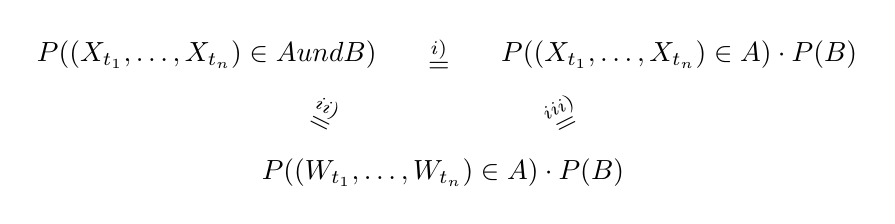
\begin{tikzpicture}
\node (A) at (0, 0) {$\displaystyle P((X_{t_1}, \ldots, X_{t_n}) \in A \text{ und } B)$};
\node (B) at (6, 0) {$\displaystyle P((X_{t_1}, \ldots, X_{t_n}) \in A) \cdot P(B)$};
\node (C) at (3, -1.5) {$\displaystyle P((W_{t_1}, \ldots, W_{t_n}) \in A) \cdot P(B)$};

\path (A) -- node[sloped] {$\stackrel{\text{i)}}{=}$} (B);
\path (A) -- node[sloped] {$\stackrel{\text{ii)}}{=}$} (C);
\path (B) -- node[sloped] {$\stackrel{\text{iii)}}{=}$} (C);
\end{tikzpicture}
\end{center}
Ist dies gezeigt, so folgt die Unabh�ngigkeit aus i) und da $(W_t)$ und $(X_t)$ nach iii) die selben Randverteilungen besitzen, ist $(X_t)$ ein zentrierter Gau�-Prozess mit Kovarianzfunktion $\Gamma(s,t) = \min\{s, t\}$. Da $(X_t)$ offensichtlich auch stetig ist, folgt nach Satz \ref{Nummer5.1.6} also, dass $(X_t)$ ein Wiener-Prozess ist. Der Beweis von i) -- iii) erfolgt nun in zwei Schritten:

Im ersten Schritt nehmen wir an, dass $\tau$ nur abz�hlbar viele Werte annimmt. Sei $\tau(\Omega)$ also abz�hlbar und $(s_n)_{n \geq 1}$ eine entsprechende Abz�hlung. F�r $n \geq 1$ und $B \in \sF_\tau$ gilt dann
\begin{align*}
B \cap \{\tau = s_n\} &= \underbrace{B \cap \{\tau \leq s_n\}}_{\in \sF_{s_n}} \cap \{\tau = s_n\}\text{,}
\end{align*}
der letzte Teil l�sst sich als $\{\tau = s_n\} = \{\tau \leq s_n\} \setminus \bigcup_{s_m < s_n} \{\tau \leq s_m\}$ schreiben l�sst. Nun ist $\{\tau \leq s_n\} \in \sF_{s_n}$ und $\{\tau \leq s_m\} \in \sF_{s_m} \subset \sF_{s_n}$, insgesamt also $B \cap \{\tau = s_n\} \in \sF_{s_n}$. Auf $\{\tau = s_n\}$ gilt nun $X_t = W_{t + \tau} - W_\tau = W_{t + s_n} - W_{s_n} =: Y_t^{(n)}$. Beachte, dass $(Y^{(n)})_{t \geq 0}$ ein Wiener-Prozess ist, der nach Korollar \ref{Nummer5.1.9} von $\sF_{s_n}$ unabh�ngig ist. Nun folgt
\begin{align*}
P((X_{t_1}, \ldots, X_{t_n}) \in A \text{ und } B) &= \sum_{n=1}^\infty P((X_{t_1}, \ldots, X_{t_n}) \in A \text{ und } B \cap \{\tau = s_n\})\\
\quad &= \sum_{n=1}^\infty P((Y_{t_1}^{(n)}, \ldots, Y_{t_n}^{(n)}) \in A \text{ und } B \cap \{\tau = s_n\})\\
\quad &= \sum_{n=1}^\infty P((Y_{t_1}^{(n)}, \ldots, Y_{t_n}^{(n)}) \in A)P(B \cap \{\tau = s_n\})\\
\quad &= \sum_{n=1}^\infty P((W_{t_1}, \ldots, W_{t_n}) \in A)P(B \cap \{\tau = s_n\})\\
\quad &= P((W_{t_1}, \ldots, W_{t_n}) \in A)P(B)\text{.}
\end{align*}
Damit ist iii) gezeigt. Setzt man $B := \Omega$, so folgt auch ii).

Im zweiten Schritt sei $\tau$ allgemein. F�r $n \in \N_0$ sei $\tau_n := \sum_{k=0}^\infty \frac{k+1}{2^n}\ind_{\{k2^{-n} \leq \tau < (k+1)2^{-n}\}}$ und $\tau_n(\omega) := \infty$, falls $\tau(\omega) = \infty$ ist. Offensichtlich ist $\tau_n(\Omega)$ abz�hlbar. Zu zeigen ist also, dass $\tau_n$ eine Stoppzeit ist. F�r $0 \leq t < 2^{-n}$ gilt $\{\tau_n \leq t\} = \emptyset \in \sF_t$. F�r $2^{-n} \leq t$ gibt es ein $k_0 \geq 0$ mit $(k_0+1)2^{-n} \leq t < (k_0+2)2^{-n}$. Dann folgt
\begin{align*}
\{\tau_n \leq t\} &= \bigcup_{k=0}^{k_0} \left\{\tau_n = \frac{k+1}{2^n}\right\} = \bigcup_{k=0}^{k_0} \underbrace{\left\{k2^{-n} \leq \tau < (k+1)2^{-n}\right\}}_{\in \sF_{(k+1)2^{-n}}}\\
\quad &\in \sF_{(k_0 + 1)2^{-n}} \subset \sF_t\text{.}
\end{align*}
Ferner ist $\tau_n \geq \tau$ und $\tau_n \searrow \tau$. F�r $n \in \N_0$ setzen wir nun $Y_t^{(n)} := W_{t + \tau_n} - W_{\tau_n}$, dann ist $Y_t^{(n)}$ gem�� dem ersten Schritt ein Wiener-Prozess. Da Wiener-Prozesse stetig sind, folgt $Y_t^{(n)} \stackrel{n \to \infty}{\longrightarrow} X_t$ $P$-fast sicher. Ferner sei $B \in \sF_\tau \subset \sF_{\tau_n}$, mit dem ersten Schritt folgt dann $P((Y_{t_1}^{(n)}, \ldots, Y_{t_m}^{(n)}) \in A \text{ und } B) = P((W_{t_1}, \ldots, W_{t_m}) \in A)P(B)$. Da $P$-fast sichere Konvergenz die Konvergenz in Verteilung impliziert, folgt insgesamt
\begin{align*}
P((X_{t_1}, \ldots, X_{t_m}) \in A)P(B) &= P((W_{t_1}, \ldots, W_{t_m}) \in A)P(B)\text{.}
\end{align*}
Damit ist wieder iii) gezeigt und ii) folgt wiederum mit $B = \Omega$.
\end{beweis}
	\section{Das Reflektionsprinzip}

Wir betrachten f�r $a > 0$ die erste Passierzeit $\tau_a := \inf\{t \geq 0 : W_t = a\}$ und wollen untersuchen, wie die Verteilung oder Verteilungsfunktion von $\tau_a$ aussieht. Wegen $P(W_t = a) = 0$ gilt zun�chst $P(\tau_a \leq t) = P(\tau_a \leq t, W_t \geq a) + P(\tau_a \leq t, W_t \leq a)$. Ferner gilt $P(\tau_a \leq t, W_t \geq a) = P(W_t \geq a)$, da mit $W_0 = 0$ $P$-fast sicher und der Stetigkeit der Pfade folgt, dass $\{W_t \geq a\} \subset \{\tau_a \leq t\}$ gilt. F�r den zweiten Summanden wollen wir nun eine heuristische Betrachtung durchf�hren:

\begin{figure}[!htbp]
\centering
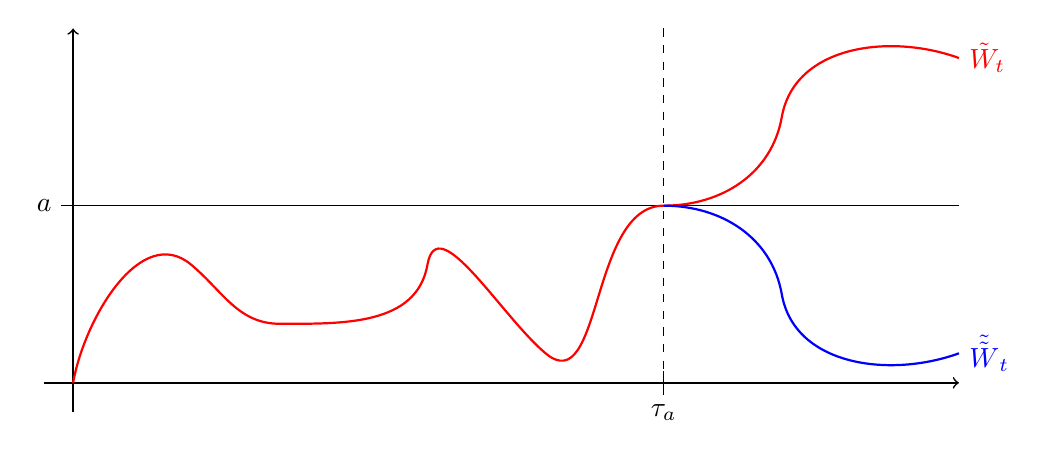
\begin{tikzpicture}[scale=0.75]
\draw[semithick, ->] (-0.5,0) -- (15,0);
\draw[semithick, ->] (0,-0.5) -- (0,6);

\draw (-0.2, 3) node[left] {$a$} -- (15, 3);
\draw (10, 0.2) -- (10, -0.2) node [below] {$\tau_a$};
\draw[dashed] (10, 6) -- (10, 0.2);

\draw[thick, red] (0, 0)   to[out=80, in=140]
									(2, 2)   to[out=-40, in=180]
									(3.5, 1) to[out=0, in=-100]
									(6, 2)   to[out=80, in=140]
									(8, 0.5) to[out=-40, in=180]
									(10, 3);
									
\draw[thick, red] (10, 3)   to[out=0, in=-100]
									(12, 4.5) to[out=80, in=160]
									(15, 5.5) node[right] {$\tilde{W}_t$};
\draw[thick, blue](10, 3)   to[out=0, in=100]
									(12, 1.5) to[out=-80, in=-160]
									(15, 0.5) node[right] {$\tilde{\tilde{W}}_t$};
\end{tikzpicture}
\caption[Neugestarteter Prozess f�r das Reflektionsprinzip]{Der Prozess wird in $\tau_a$ neugestartet und ist dann um $a$ gewisserma�en symmetrisch.}\label{fig:reflektionsprinzip}
\end{figure}

Wir starten den Wiener-Prozess in $\tau_a$ neu, nach Satz \ref{Nummer5.3.6} ist die Zukunft dann von der Vergangenheit bis $\tau_a$ unabh�ngig. Der neugestartete Wiener-Prozess ist zudem gewisserma�en um die $a$ symmetrisch, d.\,h. $W$ und $-W$ sind Wiener-Prozesse. Damit ist
\begin{align*}
P(\tau_a \leq t, W_t \leq a) &= P(\tau_a \leq t, \tilde{W}_t \leq a) \stackrel{\text{!}}{=} P(\tau_a \leq t, \tilde{\tilde{W}}_t \geq a) = P(\tilde{\tilde{W}}_t \geq a) = P(W_t \geq a)\text{.}
\end{align*}
Insgesamt gilt also $P(\tau_a \leq t) = 2P(W_t \geq a)$. Die markierte Gleichheit bei $\stackrel{\text{!}}{=}$ ist so jedoch nicht begr�ndbar, da Symmetrie eigentlich eine andere Eigenschaft ist. Um dies zu reparieren, ben�tigen wir den folgenden Satz.

\begin{satz}\label{Nummer5.4.1}
Mit den obigen Bezeichnungen ist $(\tilde{W}_t)_{t \geq 0}$ definiert durch
\begin{align*}
\tilde{W}_t &:= \begin{cases} W_t & \text{falls } t \leq \tau_a\\ 2a - W_t & \text{sonst}\end{cases}
\end{align*}
ebenfalls ein Wiener-Prozess.
\end{satz}

\begin{beweis}
Wegen Satz \ref{Nummer5.3.6} definiert $X_t := W_{t + \tau_a} - W_{\tau_a}$ einen von $\sF_{\tau_a}$ unabh�ngigen Wiener-Prozess. Damit haben $X := (X_t)$, $(-X_t)$ und $W := (W_t)$ die selben Verteilungen und es gilt $X \stackrel{[d]}{=} -X \stackrel{[d]}{=} W$. Ferner ist $X$ von der $\sF_{\tau_a}$-messbaren Zufallsvariablen $\tau_a$ unabh�ngig. Wegen $\tau_a \wedge s \leq \tau_a$ f�r $s \geq 0$ gilt $\sF_{\tau_a \wedge s} \subset \sF_{\tau_a}$ und damit ist $Y := (W_{\tau_a \wedge s})_{s \geq 0}$ nach Satz \ref{Nummer5.3.5} und Lemma \ref{Nummer5.3.4} ein $(\sF_{\tau_a \wedge s})_{s \geq 0}$-adaptierter Prozess. Wegen $\sF_{\tau_a \wedge s} \subset \sF_{\tau_a}$ ist dann $X$ von $Y$ unabh�ngig und da $(Y, \tau_a)$ von $X$ bzw. $-X$ unabh�ngig ist, erhalten wir
\begin{align*}
(Y, \tau_a, X) &\stackrel{[d]}{=} (Y, \tau_a, -X)\text{.} \tag{*}
\end{align*} 
Wir betrachten nun $C_0 := \{g \in C([0, \infty))\text{, } g(0) = 0\}$ und $\psi\colon C([0, \infty)) \times [0, \infty) \times C_0 \to C([0, \infty))$ definiert durch
\begin{align*}
\psi(f, t_0, g) &:= \begin{cases} f(t) & \text{falls } t \leq t_0\\ f(t_0) + g(t-t_0) & \text{falls } t \geq t_0\end{cases}
\end{align*}
f�r alle $t \geq 0$. Mit (*) erhalten wir dann $\psi(Y, \tau_a, X) \stackrel{[d]}{=} \psi(Y, \tau_a, -X)$. Ferner ist
\begin{align*}
\psi(Y, \tau_a, X) &= \begin{cases}W_t & \text{falls } t \leq \tau_a\\ W_{\tau_a} + X_{t-\tau_a} & \text{falls } t \geq \tau_a\end{cases}\\
\quad &= (W_t)_{t \geq 0}
\shortintertext{und analog}
\psi(Y, \tau_a, -X) &= \begin{cases}W_t & \text{falls } t \leq \tau_a\\ W_{\tau_a} - X_{t-\tau_a} & \text{falls } t \geq \tau_a\end{cases}\\
\quad &= W_{\tau_a} - W_{\tau_a + t - \tau_a} + W_{\tau_a} = 2a - W_t\\
\quad &= (\tilde{W}_t)_{t \geq 0}\text{.}
\end{align*}
Damit besitzen $(W_t)$ und $(\tilde{W}_t)$ die gleichen Verteilungen und daher ist $(\tilde{W}_t)$ ein zentrierter Gau�-Prozess mit der Kovarianzfunktion $\Gamma(s,t) = \min\{s, t\}$, der nach Konstruktion stetige Pfade besitzt, also ist er ein Wiener-Prozess.
\end{beweis}

\begin{satz}[Reflektionsprinzip]\label{Nummer5.4.2}
Sei $(W_t)$ ein Wiener-Prozess und $\tau_a$ die erste Passierzeit f�r ein $a > 0$. Dann gilt
\begin{align*}
P\left(\max_{s \in [0, t]} W_s \geq a\right) &= P(\tau_a \leq t) = P(\vert W_t \vert \geq a) = 2P(W_t \geq a)\\
\quad &= 1 - \sN(0,t)[-a,a]\text{.}
\end{align*}
\end{satz}

Man kann ferner zeigen, dass $P$-fast sicher $\tau_a < \infty$ gilt, was unmittelbar aus den Aussagen des Satzes folgt. Die Dichte von $\tau_a$ l�sst sich auch bestimmen, hierzu verweisen wir auf \cite[Satz 13.9]{MEINTRUP}. Schlie�lich l�sst sich auch $\E \tau_a = \infty$ zeigen.

\begin{information}
Satz \ref{Nummer5.4.1} wird h�ufig ebenfalls oder alternativ Reflektionsprinzip genannt.
\end{information}

\begin{beweis}
Man kann leicht zeigen, dass $\{\tau_a \leq t\} = \left\{\max_{s \in [0,t]} W_s \geq a\right\}$ gilt. Damit reicht es, zu zeigen, dass
\begin{align*}
P\left(\max_{s \in [0,t]} W_s \geq a\right) &= 2P(W_t \geq a)
\end{align*}
gilt. Dazu sei $(\tilde{W}_t)$ der Wiener-Prozess aus Satz \ref{Nummer5.4.1}. Dann gilt $\{W_t \geq a\} \subset \{\tilde{W}_t \leq a\}$ und analog f�r $>$ und $<$, denn f�r $W_t \geq a$ gilt $\tau_a \leq t$ und damit $\tilde{W}_t = 2a - W_t \leq 2a-a = a$. Ferner erhalten wir eine disjunkte Vereinigung
\begin{align*}
\left\{\max_{s \in [0,t]} W_s \geq a\right\} &= \{W_t \geq a\} \sqcup \{\tilde{W}_t > a\}\text{,}
\end{align*}
dazu sei f�r "`$\subset$"' zun�chst $s \in [0,t]$ mit $W_s \geq a$, dann gilt entweder $W_t \geq a$ und wir sind fertig oder es gilt $W_t < a$. In diesem Fall folgt mit dem Zwischenwertsatz $\tau_a \leq s \leq t$ und damit $\tilde{W}_t = 2a - W_t > 2a-a = a$. F�r "`$\supset$"' beobachten wir zun�chst, dass $\{W_t \geq a\} \subset \left\{\max_{s \in [0,t]} W_s \geq a\right\}$ offensichtlich ist. Sei nun $\tilde{W}_t > a$, dann folgt mit unseren Vor�berlegungen $W_t < a$. Damit gilt $\tilde{W}_t \neq W_t$ und aus der Definition von $\tilde{W}_t$ folgt daher $t > \tau_a$. Dann existiert ein $s \in [0,t]$ mit $W_s = a$ und daher $\max_{s \in [0,t]} W_s \geq a$. 

Damit gilt nun
\begin{align*}
P\left(\max_{s \in [0,t]} W_s \geq a\right) &= P(W_t \geq a) + P(\tilde{W}_t > a) = P(W_t \geq a) + P(\tilde{W}_t \geq a)\\
\quad &= 2P(W_t \geq a)\text{.} \qedhere
\end{align*}
\end{beweis}
	\section{Der Wiener-Prozess als Martingal}

In diesem letzten Abschnitt wollen wir eine kurze Einf�hrung in die Theorie der Martingale in stetiger Zeit geben und die Anwendung auf Wiener-Prozesse diskutieren.

\begin{definition}[Martingal]\label{Nummer5.5.1}
Ein stochastischer Prozess $(X_t)_{t \geq 0}$, der an $\sF = (\sF_t)_{t \geq 0}$ adaptiert und integrierbar ist, hei�t \deftxt{Martingal}\index{Martingal} genau dann, wenn
\begin{align*}
\E(X_t \mid \sF_s) &= X_s
\end{align*}
f�r alle $0 \leq s \leq t$ gilt. Sub- und Super-Martingale werden ebenfalls analog definiert.
\end{definition}

\begin{satz}[Unabh�ngige Zuw�chse]\label{Nummer5.5.2}
Sei $(X_t)$ ein integrierbarer, stochastischer Prozess mit unabh�ngigen Zuw�chsen. Dann ist $(X_t - \E X_t)_{t \geq 0}$ ein Martingal bez�glich der nat�rlichen Filtration. 

Insbesondere ist der Wiener-Prozess ein Martingal und $(N_t - \lambda t)_{t \geq 0}$ ist ebenfalls ein Martingal, falls $N_t$ ein homogener Poisson-Prozess mit Rate $\lambda$ ist.
\end{satz}

\begin{beweis}
Die Aussage folgt aus Lemma \ref{Nummer5.1.8} und einigen elementaren Rechnungen. 
\end{beweis}

\begin{satz}[Gleichgradig integrierbare Martingale]\label{Nummer5.5.3}
Sei $(X_t)$ ein Martingal, dann sind folgende Aussagen �quivalent:
\begin{enumerate}
	\item\label{N553A1} Der Prozess $(X_t)$ ist gleichgradig integrierbar.
	\item\label{N553A2} Es existiert $X_\infty \in \sL_1$ mit $X_t = \E(X_\infty \mid \sF_t)$ f�r alle $t \geq 0$.
\end{enumerate}
\end{satz}

\begin{beweis}
Die Richtung von \ref{N553A1} $\Rightarrow$ \ref{N553A2} ist eine Folgerung aus Satz \ref{Nummer2.7.2}, die andere Richtung folgt aus Satz \ref{Nummer2.6.4}.
\end{beweis}

\begin{satz}[Optional Sampling Theorem]\label{Nummer5.5.4}\index{Optional Sampling Theorem}
Sei $(X_t)_{t \geq 0}$ ein rechtsstetiges Martingal und $\sigma \leq \tau$ Stoppzeiten. Ist $\tau$ beschr�nkt oder $(X_t)$ gleichgradig integrierbar, so sind $X_\sigma, X_\tau \in \sL_1$ und es gilt
\begin{align*}
\E(X_\tau \mid \sF_\sigma) = X_\sigma\text{.}
\end{align*}
Dabei ist $X_\sigma$ nach Lemma \ref{Nummer5.3.4} und Satz \ref{Nummer5.3.5} $\sF_\sigma$-messbar.
\end{satz}

\begin{beweis}
Wir wollen den Beweis an dieser Stelle lediglich skizzieren. Wie im Beweis von Satz \ref{Nummer2.4.3} zeigen wir zun�chst
\begin{align*}
\E(X_N \mid \sF_\tau) &= X_\tau
\end{align*}
f�r $N \in [0, \infty]$ mit $\tau \leq N$. Dies beweist man in zwei Schritten: Zun�chst nimmt man an, dass $\tau$ abz�hlbar viele, aufsteigende Werte besitzt. Dann kann man die Aussage aus Satz \ref{Nummer2.4.3} und Satz \ref{Nummer2.8.1} folgern. Im zweiten Schritt betrachtet man allgemeine $\tau$ und approximiert diese durch $\tau_n \searrow \tau$, wobei die $\tau_n$ wie im ersten Schritt gegeben sind. Hierf�r ist die Rechtsstetigkeit n�tig. F�r die Details verweisen wir auf \cite{MEINTRUP}. Dort wird auch gezeigt, dass jedes Martingal eine rechtsstetige Version besitzt, wenn $\sA$ vervollst�ndigt wird.
\end{beweis}

\begin{korollar}[Optional Stopping Theorem (Doob)]\label{Nummer5.5.5}\index{Optional Stopping Theorem}\index{Doob!Optional Stopping Theorem}
Sei $(X_t)$ ein rechtsstetiges Martingal und $\tau$ eine Stoppzeit. Dann ist $(X_{\tau \wedge t})_{t \geq 0}$ ein Martingal. Ist $\tau$ beschr�nkt oder $(X_t)$ gleichgradig integrierbar, so gilt $X_\tau \in \sL_1$ und $\E X_\tau = \E X_0$.
\end{korollar}

\begin{beweis}
Die Martingaleigenschaft folgt aus Satz \ref{Nummer5.5.4} f�r die beschr�nkten Stoppzeiten $\tau \wedge s$ und $\tau \wedge t$. Die zweite Aussage folgt aus Satz \ref{Nummer5.5.4} f�r $\sigma = 0$, denn dann ist $\E(X_\tau \mid \sF_0) = X_0$ und damit $\E X_\tau = \E(\E(X_\tau \mid \sF_0)) = \E X_0$.
\end{beweis}

\begin{satz}[Wiener-Prozesse und Martingale]\label{Nummer5.5.6}
Sei $(W_t)$ ein Wiener-Prozess. Dann sind $(W_t)$ und $(W_t^2 - t)$ stetige Martingale.
\end{satz}

Es lassen sich auch andere Transformationen betrachten, die (stetige) Martingale ergeben. Hierzu verweisen wir auf \cite[13.10 und 13.11]{MEINTRUP}.

\begin{beweis}
Die Aussagen folgen aus Satz \ref{Nummer5.5.2} und einfachem Nachrechnen.
\end{beweis}

\begin{korollar}[Ruinwahrscheinlichkeiten des Wiener-Prozesses]\label{Nummer5.5.7}
Sei $(W_t)$ ein Wiener-Prozess und $a < 0 < b$. Wir setzen $\tau := \inf\{t \geq 0 : W_t = a \text{ oder } W_t = b\}$. Dann gilt
\begin{enumerate}
	\item $\displaystyle P(W_\tau = a) = \frac{b}{b-a}$.
	\item $\displaystyle \E \tau = -ab$.
\end{enumerate}
\end{korollar}

\begin{beweis}
Der Beweis verl�uft weitgehend analog zur symmetrischen Irrfahrt aus Beispiel \ref{Nummer2.4.2}. F�r die Details verweisen wir auf \cite[S. 381 ff.]{MEINTRUP}. 
\end{beweis}

Der Wiener-Prozess l�sst sich durch "`Irrfahrten"' approximieren: Sind $(Y_i)$ i.\,i.\,d. Zufallsvariablen mit $\E Y_i = 0$ und $\Var Y_i =: \sigma \in (0, \infty)$, so setzen wir f�r $t \geq 0$
\begin{align*}
s_t^{(n)} &:= \sum_{i=1}^{\lfloor nt \rfloor} Y_i \qquad\text{ und }\qquad \tilde{s}_t^{(n)} := \frac{1}{\sqrt{\sigma^2 n}}s_t^{(n)}\text{.}
\end{align*}
Das \deftxt{Donskersche Invarianzprinzip} besagt dann, dass $\tilde{s}^{(n)}$ gegen einen Wiener-Prozess konvergiert. Wie diese Konvergenz und der Wiener-Prozess aussehen wollen wir hier nicht erl�utern und verweisen auf \cite{KLENKE}.

Der Wiener-Prozess l�sst sich auch als Fourierreihe mit zuf�lligen Koeffizienten darstellen. Diese Koeffizienten sind unabh�ngig und normalverteilt. Eine m�gliche Orthonormalbasis l�sst sich explizit darstellen.

Der Satz vom iterierten Logarithmus besagt
\begin{align*}
\lim_{t \to \infty} \sup \frac{\vert W_t \vert}{\sqrt{2t \log \log t}} &= 1 \quad P\text{-fast sicher.}
\end{align*}

Ferner gibt es ein Gesetz der gro�en Zahlen, welches
\begin{align*}
\lim_{t \to \infty} \frac{W_t}{t} &= 0 = \E W_0 \quad P\text{-fast sicher}
\end{align*}
besagt. Insbesondere ist $(t W_\frac{1}{t})_{t \geq 0}$ wieder ein Wiener-Prozess.
% ================================

% Verschiebung:
% 3.2.4 -> 3.2.5 und folgende
% 3.4.12 -> ...?
% 5.1.2 -> 5.1.3 aufpassen!

\ifthenelse{\equal{\useThumbs}{1}}
	{\ihead[]{}}{}
\ifthenelse{\equal{\useIndex}{1}}{
\cleardoublepage
\cleardoublepage\begin{thebibliography}{WT}
\bibitem[Kallenberg01]{KALL} O. Kallenberg, \emph{Foundations of Modern Probability}, Springer, 2001
\bibitem[Klenke06]{KLENKE} A. Klenke, \emph{Wahrscheinlichkeitstheorie}, Springer, 2006
\bibitem[Krylov02]{KRYLOV} N. V. Krylov, \emph{Introduction to the Theory of Random Processes}, AMS: Graduate Studies in Mathematics, 2002
\bibitem[Meintrup04]{MEINTRUP} D. Meintrup und S. Sch�ffler, \emph{Stochastik -- Theorie und Anwendungen}, Springer, 2004
\bibitem[WTSkript11]{WT} I. Steinwart, \emph{Wahrscheinlichkeitstheorie}, Mitschrieb der Vorlesung "`Wahrscheinlichkeitstheorie"' von Ingo B�rk, Wintersemester 2010/2011
\bibitem[Kestelman60]{KESTELMAN} Kestelman, \emph{Modern Theory of Integration}, 1960
\bibitem[Graves56]{GRAVES} Graves, \emph{The Theory of Functions of Real Variables}, 1956 
\end{thebibliography}
\cleardoublepage
\phantomsection
\addcontentsline{toc}{chapter}{\listfigurename}
\listoffigures
\cleardoublepage
\appendix
\chapter{Anhang}
\renewcommand*{\thetmpsatz}{\thechapter.\arabic{tmpsatz}}
\setcounter{tmpsatz}{0}
An dieser Stelle wollen wir einige wichtige S�tze aus anderen Vorlesungen festhalten, wie mehrmals ben�tigt und referenziert werden. Da diese nur der �bersicht dienen, werden wir auf Beweise dieser S�tze an dieser Stelle verzichten.

\begin{satz}[Totale Wahrscheinlichkeit]\label{appendix:totwkeit}
Sei $(\Omega, \sA, P)$ ein Wahrscheinlichkeitsraum und $(B_i)_{i \in I}$ eine h�chstens abz�hlbare Zerlegung von $\Omega$. Ferner gelte $P(B_i) > 0$ f�r alle $i \in I$. F�r alle $A \in \sA$ gilt dann
\begin{align*}
P(A) &= \sum_{i \in I} P(B_i)P(A \mid B_i)\text{.}
\end{align*}
\end{satz}

\begin{beweis}
Der Beweis findet sich in \cite[Satz I.7.3]{WT}.
\end{beweis}

\begin{satz}[Beppo Levi I / Monotone Konvergenz]\label{appendix:beppolevi1}
Es sei $(\Omega, \sA, \mu)$ ein Ma�raum und $f_n\colon \Omega \to [0, \infty]$ f�r $n \geq 1$ eine Folge messbarer Funktionen mit $f_n \nearrow f$. Dann folgt, dass $f$ messbar und nicht-negativ ist. Au�erdem gilt
\begin{align*}
\int f~\dd \mu &= \lim_{n \to \infty} \int f_n~\dd \mu = \sup_{n \geq 1} \int f_n~\dd \mu\text{.}
\end{align*}
\end{satz}

\begin{beweis}
Der Beweis findet sich in \cite[Satz I.11.13]{WT}.
\end{beweis}

%\begin{satz}[Beppo Levi II]\label{appendix:beppolevi2}
%Es sei $(\Omega, \sA, \mu)$ ein Ma�raum und $(f_n) \subset \sL^1(\mu)$ eine Folge integrierbarer Funktionen, so dass $\mu$-fast �berall $f_n \nearrow f$ f�r eine Abbildung $f\colon \Omega \to \R$ gilt. Dann folgt
%\begin{align*}
%\lim_{n \to \infty} \int f_n~\dd\mu &= \int f~\dd\mu = \int f^+~\dd\mu - \int f^-~\dd\mu\text{.}
%\end{align*}
%\end{satz}
%
%\begin{beweis}
%Der Beweis findet sich in \cite[Satz I.11.13]{WT}.
%\end{beweis}

\begin{lemma}[Fatou]\label{appendix:fatou}
Es sei $(\Omega, \sA, \mu)$ ein Ma�raum und $f_n\colon \Omega \to [0, \infty]$ f�r $n \geq 1$ eine messbare Funktionenfolge. Dann gilt
\begin{align*}
\int \liminf_{n \to \infty} f_n~\dd\mu &\leq \liminf_{n \to \infty} \int f_n~\dd \mu\text{.}
\end{align*}
\end{lemma}

\begin{beweis}
Der Beweis findet sich in \cite[Lemma I.11.14]{WT}.
\end{beweis}

\begin{satz}[Lebesgue / Dominierte Konvergenz]\label{appendix:lebesgue}
Es sei $(\Omega, \sA, \mu)$ ein Ma�raum, $f_n\colon \Omega \to \R \cup \{\pm\infty\}$ f�r $n \geq 1$ eine Folge messbarer Funktionen und $f, g\colon \Omega \to \R \cup \{\pm\infty\}$ messbare Abbildungen mit $f_n \to f$ und $|f_n| \leq g$ f�r alle $n \geq 1$. Ist $g$ bez�glich $\mu$ integrierbar, so gilt dies auch f�r $f$ und es folgt
\begin{align*}
\int \lim_{n \to \infty} f_n~\dd\mu &= \int f~\dd\mu = \lim_{n \to \infty} \int f_n~\dd\mu\text{.}
\end{align*}
\end{satz}

\begin{beweis}
Der Beweis findet sich in \cite[Lemma I.11.16]{WT}.
\end{beweis}

\begin{lemma}[Borel-Cantelli II]\label{appendix:borelcantelli2}
Es sei $(\Omega, \sA, P)$ ein Wahrscheinlichkeitsraum und $(A_n)_{n \geq 1} \subset \sA$ unabh�ngig. Dann gilt
\begin{align*}
\sum_{n=1}^\infty P(A_n) = \infty &\Longrightarrow P\left(\limsup_{n \to \infty} A_n\right) = 1\text{.}
\end{align*}
F�r unabh�ngige Folgen $(A_n)_{n \geq 1} \subset \sA$ gilt damit insbesondere $P(\limsup A_n) \in \{0,1\}$ und $P(\liminf A_n) \in \{0,1\}$.
\end{lemma}

\begin{beweis}
Der Beweis findet sich in \cite[Lemma II.6.1]{WT}.
\end{beweis}
\cleardoublepage
\renewcommand{\indexname}{Stichwortverzeichnis}
\printindex}{}
\end{document}